% !TEX program = xelatex
% 编译：xelatex furry_qcd.tex（运行两次以生成目录与交叉引用）
% 字体：fontset=fandol 随 TeX Live 发行，可在任何平台编译；
%       在 macOS 上可改为 fontset=macnew 以获得更好的中文字体效果。
\documentclass[UTF8,a4paper,11pt,fontset=fandol]{ctexart}

\usepackage[margin=2.5cm,headheight=14pt]{geometry}
\usepackage{amsmath,amssymb,amsthm,mathtools,bm}
% \mathbb 1：amssymb 的 msbm 字体没有数字 1，改用 dsfont 的 \mathds{1}；\mathbb{C}、\mathbb{R} 等不变
\usepackage{dsfont}
\let\amsmathbb\mathbb
\renewcommand{\mathbb}[1]{\ifx1#1\mathds{1}\else\amsmathbb{#1}\fi}
\usepackage{slashed}
\usepackage{booktabs,array,multirow,tabularx}
\usepackage{enumitem}
\usepackage{caption,subcaption}
\captionsetup{labelsep=quad}     % 图表标题 “图 5　……”：编号后空一字，不用西文冒号
\usepackage[section]{placeins}   % 浮动体不越过 \section 边界
\usepackage[dvipsnames]{xcolor}
\usepackage{tikz}
\usetikzlibrary{decorations.pathmorphing,decorations.markings,arrows.meta,calc,positioning}
\usepackage[most]{tcolorbox}
\usepackage{etoolbox}            % \patchcmd、\appto（tcolorbox 亦载入，此处显式声明）
\usepackage[colorlinks=true,linkcolor=blue!50!black,citecolor=green!40!black,
            urlcolor=blue!60!black,bookmarksnumbered=true]{hyperref}
\usepackage[nameinlink]{cleveref}
\usepackage[nottoc]{tocbibind}   % 参考文献进入目录与 PDF 书签

% ---------------- 定理类环境 ----------------
% 定理、引理、命题、推论的正文：汉字用楷体，西文保持直立。plain 样式的 \itshape
% 会把对称性名称 “C 宇称/C 偶/C 奇” 中的正体 C 排成斜体，与电荷共轭矩阵 $C$
% 无法区分；上下间距与标题字体同 plain。
% 三种样式的标题都按中文习惯排：附注用全角括号（……），标题后不加西文句点而空一字；
% cdefinition、cremark 的字体与上下间距分别同 amsthm 的 definition、remark 样式。
\newtheoremstyle{cplain}{\topsep}{\topsep}{\kaishu}{0pt}{\bfseries}{}{1em}%
  {\thmname{#1}\thmnumber{ \textup{#2}}\thmnote{\normalfont（#3）}}
\newtheoremstyle{cdefinition}{\topsep}{\topsep}{\normalfont}{0pt}{\bfseries}{}{1em}%
  {\thmname{#1}\thmnumber{ \textup{#2}}\thmnote{\normalfont（#3）}}
\newtheoremstyle{cremark}{\glueexpr\topsep/2\relax}{\glueexpr\topsep/2\relax}%
  {\normalfont}{0pt}{\itshape}{}{1em}%
  {\thmname{#1}\thmnumber{ \textup{#2}}\thmnote{\normalfont（#3）}}
\theoremstyle{cplain}
\newtheorem{theorem}{定理}[section]
\newtheorem{lemma}[theorem]{引理}
\newtheorem{proposition}[theorem]{命题}
\newtheorem{corollary}[theorem]{推论}
\theoremstyle{cdefinition}
\newtheorem{definition}[theorem]{定义}
\newtheorem{example}[theorem]{例}
\theoremstyle{cremark}
\newtheorem{remark}[theorem]{注}
\renewcommand{\proofname}{证明}
% 证明的标题同样不加句点：amsthm 原定义中的 \@addpunct{.} 改为 0.5em，连同 \labelsep 共空一字
\makeatletter
\renewenvironment{proof}[1][\proofname]{\par\pushQED{\qed}\normalfont\topsep6\p@\@plus6\p@\relax
  \trivlist\item[\hskip\labelsep\itshape #1\hspace{0.5em}]\ignorespaces}{\popQED\endtrivlist\@endpefalse}
\makeatother

\tcolorboxenvironment{theorem}{enhanced,breakable,colback=blue!3!white,
  colframe=blue!45!black,boxrule=0.6pt,arc=2pt,left=5pt,right=5pt,top=3pt,bottom=3pt}

\crefname{theorem}{定理}{定理}
\crefname{lemma}{引理}{引理}
\crefname{proposition}{命题}{命题}
\crefname{corollary}{推论}{推论}
\crefname{definition}{定义}{定义}
\crefname{example}{例}{例}
\crefname{remark}{注}{注}
\crefname{equation}{式}{式}
\creflabelformat{equation}{#2(#1)#3}
\crefname{figure}{图}{图}
\crefname{table}{表}{表}
\crefformat{section}{#2第~#1~节#3}
\crefformat{subsection}{#2第~#1~小节#3}
\crefformat{appendix}{#2附录~#1#3}
\crefformat{subappendix}{#2附录~#1#3}
\Crefformat{section}{#2第~#1~节#3}
\Crefformat{subsection}{#2第~#1~小节#3}
\Crefformat{appendix}{#2附录~#1#3}
\Crefformat{subappendix}{#2附录~#1#3}
% 多目标引用的中文连接词
\newcommand{\crefpairconjunction}{与}
\newcommand{\crefmiddleconjunction}{、}
\newcommand{\creflastconjunction}{与}
\newcommand{\crefpairgroupconjunction}{与}
\newcommand{\crefmiddlegroupconjunction}{、}
\newcommand{\creflastgroupconjunction}{与}
\newcommand{\crefrangeconjunction}{至}

% \cref 后紧跟汉字时补中西文间距：xeCJK 不能越过超链接的边界自动插入 \CJKecglue
% （源文件中 \cref 与汉字之间不留空格），此处手工补上。
% 最后一组引用若为 section/subsection 类型（“第 n 节/小节”，以汉字结尾）则不补。
\ExplSyntaxOn
\NewCommandCopy \__furry_cref_orig:w \cref
\tl_new:N \l__furry_cref_type_tl
\seq_new:N \l__furry_cref_types_seq
% 标签 #1 的 cleveref 类型，取自 \r@#1@cref = {[类型][..][..]..}{..}；标签未定义时为空
\cs_new:Npn \__furry_cref_type:n #1
  {
    \cs_if_exist:cT { r@ #1 @cref }
      { \exp_last_unbraced:Nv \__furry_cref_type_aux:w { r@ #1 @cref } \q_stop }
  }
\cs_new:Npn \__furry_cref_type_aux:w #1#2 \q_stop
  { \__furry_cref_type_auxii:w #1 [] \q_stop }
\cs_new:Npn \__furry_cref_type_auxii:w #1 [#2] #3 \q_stop
  { \tl_if_empty:nT {#1} {#2} }
% 输出中最后一组引用的类型（cleveref 默认按各类型首次出现的次序分组输出）
\cs_new_protected:Npn \__furry_cref_last_type:n #1
  {
    \seq_clear:N \l__furry_cref_types_seq
    \clist_map_inline:nn {#1}
      {
        \tl_set:Nx \l__furry_cref_type_tl { \__furry_cref_type:n {##1} }
        \seq_if_in:NVF \l__furry_cref_types_seq \l__furry_cref_type_tl
          { \seq_put_right:NV \l__furry_cref_types_seq \l__furry_cref_type_tl }
      }
    \seq_get_right:NNF \l__furry_cref_types_seq \l__furry_cref_type_tl
      { \tl_clear:N \l__furry_cref_type_tl }
  }
% 下一记号若为 CJK 统一汉字（U+3400--U+9FFF），在其前插入 \CJKecglue
\cs_new_protected:Npn \__furry_cref_ecglue:N #1
  {
    \bool_lazy_all:nTF
      {
        { \token_if_letter_p:N #1 }
        { ! \token_if_cs_p:N #1 }
        { \int_compare_p:nNn { `#1 } > { "33FF } }
        { \int_compare_p:nNn { `#1 } < { "A000 } }
      }
      { \CJKecglue #1 }
      { #1 }
  }
\RenewDocumentCommand \cref { s m }
  {
    \IfBooleanTF {#1}
      { \__furry_cref_orig:w * {#2} }
      { \__furry_cref_orig:w {#2} }
    \__furry_cref_last_type:n {#2}
    \str_case:VnF \l__furry_cref_type_tl
      { { section } { } { subsection } { } }
      { \peek_N_type:TF { \__furry_cref_ecglue:N } { } }
  }
\ExplSyntaxOff

\numberwithin{equation}{section}

% 标题中的数学式随标题加粗（含目录中节一级条目）
\ctexset{section/format+=\boldmath,subsection/format+=\boldmath,paragraph/format+=\boldmath}
\makeatletter
\patchcmd{\l@section}{\bfseries}{\bfseries\boldmath}{}%
  {\@latex@warning@no@line{\string\l@section\space not patched: math in TOC section entries stays non-bold}}
\makeatother

% 目录行距略紧并单独成页（正文从新页开始）
\let\furryorigtableofcontents\tableofcontents
\renewcommand{\tableofcontents}{%
  \begingroup\linespread{1.1}\selectfont\furryorigtableofcontents\endgroup\clearpage}

% 参考文献条目间距略紧。\parsep 须在列表参数中设定（\list 随即把它赋给 \parskip），
% 故写入 thebibliography 在列表参数中执行的 \@openbib@code，而不追加在 \thebibliography 之后
\makeatletter
\appto\@openbib@code{\setlength{\itemsep}{1pt plus 1pt}\setlength{\parsep}{0pt}}
\makeatother

% 页眉：节标题不转为大写（避免 “DIRAC”“FURRY” 之类）；页眉一律用直立体（含目录、
% 参考文献页）：headings 样式原以 \slshape 排页眉，而 FandolSong 没有倾斜体，汉字会
% 退成楷体，西文则倾斜
\makeatletter
\renewcommand{\sectionmark}[1]{\markright{\ifnum\c@secnumdepth>\m@ne\thesection\quad\fi #1}}
\def\@oddhead{{\upshape\rightmark}\hfil\thepage}
\makeatother

% ---------------- 记号宏 ----------------
\DeclareMathOperator{\Tr}{Tr}
\DeclareMathOperator{\Real}{Re}
\DeclareMathOperator{\Imag}{Im}
\newcommand{\TrD}{\operatorname{Tr}_{\mathrm{D}}}   % Dirac 迹
\newcommand{\Trc}{\operatorname{Tr}_{\mathrm{c}}}   % 色迹
\newcommand{\sla}[1]{\slashed{#1}}                  % Feynman slash
\newcommand{\dd}{\mathrm{d}}                         % 微分符号
\newcommand{\tp}{\mathsf{T}}                         % 转置
\newcommand{\Cop}{\mathcal{C}}                       % Hilbert 空间上的电荷共轭算符
\newcommand{\Rop}{\mathcal{R}}                       % C 在色张量上的作用
\newcommand{\Pp}{\mathcal{P}_{+}}                    % C 偶投影
\newcommand{\Pm}{\mathcal{P}_{-}}                    % C 奇投影
\newcommand{\SF}{S_{F}}                              % 坐标空间夸克传播子
\newcommand{\su}{\mathfrak{su}}
\newcommand{\ii}{\mathrm{i}}                        % 虚数单位（正体）
\newcommand{\ee}{\mathrm{e}}                        % 自然对数底（正体）
\newcommand{\Cconj}[1]{\widetilde{#1}}              % Clifford 共轭  C X^T C^{-1}

% ---------------- TikZ 费曼图样式（纯 TikZ，不依赖 tikz-feynman） ----------------
%%% BEGIN STYLES
% =====================================================================
%  Plain-TikZ Feynman-diagram styles (no tikz-feynman).
%  Load in the preamble, after \usepackage{tikz}:
%    \usetikzlibrary{decorations.pathmorphing,decorations.markings,arrows.meta,calc,positioning}
%  Contents of this block (all low-level names start with \fd):
%   (i)  helper registers/macros and three decorations
%          "fd gluon"      coil for open paths,
%          "fd gluon loop" coil for closed paths (full circles),
%          "fd photon"     sine wave;
%        they rescale the nominal segment length so that an integer
%        number of coils / half-waves fits the path exactly (no straight
%        left-overs, evenly spaced coils, also on arcs);
%   (ii) a single \tikzset with the user-level styles:
%          fd             picture style (line width, caps, label font)
%          quark[=pos]    solid line, centred Stealth arrow at pos (default 0.5)
%          gluon          coiled line;   gluon loop[=m]: closed coil, number
%                         of coils a multiple of m (use for full circles)
%          photon         wavy line
%          ghost[=pos]    dotted line with centred arrow
%          mom={..}, mom'={..}   momentum arrow parallel to a path, on its
%                         left / right:  \path[mom={$p$}] (A) -- (B);
%                         keys: mom pos, mom length, mom sep
%          vertex         vertex dot (node style):  \node[vertex] at (A) {};
%          blob           grey filled region:  \draw[blob] (c) circle[radius=5mm];
%          bound state    double line (e.g. a bound state)
% =====================================================================
\newdimen\fdAA \newdimen\fdTW \newdimen\fdHW
\def\fdloopmult{1}
\def\fdpt#1#2#3{\pgfqpoint{\dimexpr#1\fdAA+#3\fdTW\relax}{#2\pgfdecorationsegmentamplitude}}
\def\fdcoilfull{%
  \pgfpathcurveto{\fdpt{0}{0.555}{1}}{\fdpt{0.445}{1}{2}}{\fdpt{1}{1}{3}}%
  \pgfpathcurveto{\fdpt{1.555}{1}{4}}{\fdpt{2}{0.555}{5}}{\fdpt{2}{0}{6}}%
  \pgfpathcurveto{\fdpt{2}{-0.555}{7}}{\fdpt{1.555}{-1}{8}}{\fdpt{1}{-1}{9}}%
  \pgfpathcurveto{\fdpt{0.445}{-1}{10}}{\fdpt{0}{-0.555}{11}}{\fdpt{0}{0}{12}}}
\def\fdcoilhalf{%
  \pgfpathcurveto{\fdpt{0}{0.555}{1}}{\fdpt{0.445}{1}{2}}{\fdpt{1}{1}{3}}%
  \pgfpathcurveto{\fdpt{1.555}{1}{4}}{\fdpt{2}{0.555}{5}}{\fdpt{2}{0}{6}}}
\def\fdcoilopeninit{%
  \fdAA=\pgfdecorationsegmentaspect\pgfdecorationsegmentamplitude\relax
  \pgfmathsetmacro\fdN{max(1,round((\pgfdecoratedpathlength-2*\fdAA)/\pgfdecorationsegmentlength-0.5))}%
  \pgfmathsetlength\pgfdecorationsegmentlength{(\pgfdecoratedpathlength-2*\fdAA-0.3pt)/(\fdN+0.5)}%
  \fdTW=0.0833333\pgfdecorationsegmentlength\relax}%
\def\fdcoilclosedinit{%
  \fdAA=\pgfdecorationsegmentaspect\pgfdecorationsegmentamplitude\relax
  \pgfmathsetmacro\fdN{\fdloopmult*max(1,round(\pgfdecoratedpathlength/(\fdloopmult*\pgfdecorationsegmentlength)))}%
  \pgfmathsetlength\pgfdecorationsegmentlength{(\pgfdecoratedpathlength-0.1pt)/\fdN}%
  \fdTW=0.0833333\pgfdecorationsegmentlength\relax}%
\def\fdphotoninit{%
  \pgfmathsetmacro\fdN{max(1,round(2*\pgfdecoratedpathlength/\pgfdecorationsegmentlength))}%
  \pgfmathsetlength\fdHW{(\pgfdecoratedpathlength-0.1pt)/\fdN}}%
\pgfdeclaredecoration{fd gluon}{init}{%
  \state{init}[width=+0pt,next state=coil,persistent precomputation=\fdcoilopeninit]{}%
  \state{coil}[switch if less than=1.5\pgfdecorationsegmentlength+2\fdAA to last,
               width=+\pgfdecorationsegmentlength]{\fdcoilfull}%
  \state{last}[width=+\dimexpr.5\pgfdecorationsegmentlength+2\fdAA\relax,next state=final]{\fdcoilhalf}%
  \state{final}{\pgfpathlineto{\pgfpointdecoratedpathlast}}}
\pgfdeclaredecoration{fd gluon loop}{init}{%
  \state{init}[width=+0pt,next state=coil,persistent precomputation=\fdcoilclosedinit]{}%
  \state{coil}[switch if less than=+\pgfdecorationsegmentlength to final,
               width=+\pgfdecorationsegmentlength]{\fdcoilfull}%
  \state{final}{\pgfpathlineto{\pgfpointdecoratedpathlast}}}
\pgfdeclaredecoration{fd photon}{init}{%
  \state{init}[width=+0pt,next state=up,persistent precomputation=\fdphotoninit]{}%
  \state{up}[switch if less than=+\fdHW to final,width=+\fdHW,next state=down]{%
    \pgfpathsine{\pgfqpoint{.5\fdHW}{\pgfdecorationsegmentamplitude}}%
    \pgfpathcosine{\pgfqpoint{.5\fdHW}{-\pgfdecorationsegmentamplitude}}}%
  \state{down}[switch if less than=+\fdHW to final,width=+\fdHW,next state=up]{%
    \pgfpathsine{\pgfqpoint{.5\fdHW}{-\pgfdecorationsegmentamplitude}}%
    \pgfpathcosine{\pgfqpoint{.5\fdHW}{\pgfdecorationsegmentamplitude}}}%
  \state{final}{\pgfpathlineto{\pgfpointdecoratedpathlast}}}
\tikzset{
  /pgf/decoration/coil multiple/.store in=\fdloopmult,
  fd/.style={line width=0.8pt,line cap=round,line join=round,font=\small},
  fd arrow/.style={postaction={decorate,solid,line width=0.8pt,decoration={markings,
      mark=at position #1 with {\arrow[xshift=2.9pt]{Stealth[length=5.5pt,width=4.5pt]}}}}},
  quark/.style={draw,solid,line width=0.8pt,fd arrow=#1},
  quark/.default=0.5,
  plain/.style={draw,solid,line width=0.8pt},
  gluon/.style={draw,solid,line width=0.75pt,decorate,
      decoration={fd gluon,amplitude=3.2pt,segment length=4.6pt,aspect=0.7}},
  gluon loop/.style={draw,solid,line width=0.75pt,decorate,
      decoration={fd gluon loop,amplitude=3.2pt,segment length=4.6pt,aspect=0.7,coil multiple=#1}},
  gluon loop/.default=1,
  photon/.style={draw,solid,line width=0.8pt,decorate,
      decoration={fd photon,amplitude=2pt,segment length=6.6pt}},
  ghost/.style={draw,line width=1.3pt,line cap=round,dash pattern=on 0pt off 2.6pt,fd arrow=#1},
  ghost/.default=0.5,
  mom pos/.store in=\fdmompos,mom pos=0.5,
  mom length/.store in=\fdmomlen,mom length=0.55cm,
  mom sep/.store in=\fdmomsep,mom sep=0.25cm,
  mom arrow/.style={draw,solid,line width=0.5pt,-{Stealth[length=3.8pt,width=3.2pt]}},
  mom/.style={decorate,decoration={markings,mark=at position \fdmompos with {%
      \draw[mom arrow] (-0.5*\fdmomlen,\fdmomsep) -- node[auto,inner sep=1.5pt]{#1} (0.5*\fdmomlen,\fdmomsep);}}},
  mom'/.style={decorate,decoration={markings,mark=at position \fdmompos with {%
      \draw[mom arrow] (-0.5*\fdmomlen,-\fdmomsep) -- node[auto,swap,inner sep=1.5pt]{#1} (0.5*\fdmomlen,-\fdmomsep);}}},
  vertex/.style={circle,fill,draw=none,inner sep=0pt,minimum size=3.8pt},
  blob/.style={draw,solid,fill=gray!30,line width=0.8pt},
  bound state/.style={draw,solid,double,double distance=1.6pt,line width=0.6pt},
}
%%% END STYLES

\hypersetup{pdftitle={QCD 中的 Furry 定理：严格证明与推广}}
\title{QCD 中的 Furry 定理：严格证明与推广}
\author{}
\date{\today}

\begin{document}

\maketitle

\begin{abstract}
Furry 定理断言：在量子电动力学中，含奇数个光子顶点的闭合费米子圈的两种取向互相抵消。本文对量子色动力学（QCD）给出该定理的精确表述与完整证明。
由于胶子携带色荷，电荷共轭在胶子场上的作用是 $A_\mu\to-A_\mu^{\tp}$ 而不是 $A_\mu\to-A_\mu$；夸克圈的反向圈即反夸克圈；对只含胶子顶点的夸克圈，两种取向之和只消去色迹的 C~奇部分（例如 $d^{abc}$），
而 C~偶部分（例如 $f^{abc}$）保留且一般不为零。我们在三个层次上证明这一结论：单个夸克圈的反向公式（主定理 I），它对顶点位置逐点成立，适用于四维、Pauli--Villars 正规化与维数正规化；
微扰论任意阶的选择定则 $\Rop G=(\prod_j\eta_j)\,G$（主定理 II；$\Rop$ 为电荷共轭在 Green 函数 $G$ 的外伴随色指标上的作用，$\eta_j$ 为各色单态算符的 C~宇称），其证明基于带标号 Wick 缩并上的整体反向对合；以及有限格点上的非微扰选择定则（主定理 III）。
单圈三胶子顶点的显式计算（含 Slavnov--Taylor 恒等式与紫外极点）验证了上述结论。文中还讨论了重夸克偶素衰变、色序振幅的反射恒等式与 C~奇胶子态，并明确列出本文不主张的内容。
\end{abstract}

\tableofcontents

%% ======================================================================
%% 第 1 节  引言
%% ======================================================================
\section{引言}\label{sec:intro}

Furry 定理\cite{Furry1937}是量子电动力学（QED）中最早被认识的对称性选择定则之一，常被简述为“含奇数个光子顶点的闭合费米子圈为零”。
把其中的光子换成胶子，这句话在量子色动力学（QCD）中就是错误的：胶子携带色荷，含奇数个胶子顶点的夸克圈一般并不为零。例如单圈三胶子顶点中两个夸克三角图之和正比于 $f^{abc}$，
其紫外极点正比于树图三胶子顶点\cite{DavydychevOslandSaks2001}，并对重整化常数 $Z_1$ 与 $\beta$ 函数的夸克部分有贡献（\cref{sec:triangle}）。
那么，QCD 中的 Furry 定理究竟断言什么？它在什么假设下成立？在单个夸克圈、微扰论任意阶与非微扰这三个层次上，它的确切内容分别是什么？
本文对这些问题给出完整、严格且自包含的回答：主要结论都在正文或附录中给出证明，或者明确地引自文献；少数附带讨论的推广（如复合算符的重整化，\cref{rem:reg-composite}；
含动力学光子的情形，\cref{rem:thmII-scope}；夸克偶素选择定则的任意阶形式，\cref{rem:app-onium-allorders}）只给出论证要点。

%% ----------------------------------------------------------------------
\subsection{背景：QED 中的 Furry 定理}\label{sec:intro-qed}

1937 年，Furry 在正电子理论（即今天的 QED）中证明\cite{Furry1937}：由于正、负电子之间的对称性，真空中的闭合电子圈与奇数个电磁场顶点相耦合的贡献为零。
用 Feynman 图的语言（参见\cite[第~10.1~节]{PeskinSchroeder1995}），设闭合费米子圈 $\ell$ 上有 $k$ 个光子顶点 $-\ii eQ\gamma^{\mu_j}$（$Q$ 为以 $e$ 为单位的电荷），
$\bar\ell$ 为把费米子箭头整体反向所得的反向圈（\cref{def:loop-factor}）。两种取向带有相同的电荷因子 $Q^k$ 与相同的闭合圈符号 $-1$（\cref{lem:closed-loops}），
而 Dirac 因子满足 $K_{\bar\ell}=(-1)^kK_\ell$（坐标空间中逐点成立，动量空间中须采用镜像动量配置，见\cref{prop:loop-reversal}）：
Clifford 共轭 $\Cconj X=CX^{\tp}C^{-1}$ 是保持迹的反自同构，它反转圈上矩阵乘积的次序（这正是把圈反向），并且 $\Cconj{\gamma^\mu}=-\gamma^\mu$、$\Cconj{S(p)}=S(-p)$。于是当 $k\ge3$ 时（\cref{cor:qed}）
\begin{equation}\label{eq:intro-qed}
L_\ell+L_{\bar\ell}=-(-\ii eQ)^k\,K_\ell\,\bigl[1+(-1)^k\bigr],
\end{equation}
即奇数个光子顶点的圈在两种取向之间严格相消，偶数个光子顶点的圈则两种取向相等而相加；$k=1$ 时 $\bar\ell=\ell$，关系 $K_{\bar\ell}=(-1)^kK_\ell$ 成为一致性条件 $K_\ell=-K_\ell$；$\SF(0)$ 须先正规化，在 C~相容的正规化中这一条件成立，故 $K_\ell=0$（\cref{rem:thmI-short-loops}）。
其根源是 QED 的 C~不变性（参见\cite{ItzyksonZuber1980,WeinbergQTF1}）：在 $\psi\to C\bar\psi^{\tp}$、$\bar\psi\to-\psi^{\tp}C^{-1}$、$A_\mu\to-A_\mu$ 下拉氏量不变，光子是 C~奇的。若真空是 C~不变的，便有
\begin{equation}\label{eq:intro-qed-green}
\bigl\langle0\bigm|\mathrm T\,A_{\mu_1}(x_1)\cdots A_{\mu_n}(x_n)\bigm|0\bigr\rangle
=(-1)^n\bigl\langle0\bigm|\mathrm T\,A_{\mu_1}(x_1)\cdots A_{\mu_n}(x_n)\bigm|0\bigr\rangle ,
\end{equation}
即含奇数个光子场的 Green 函数在 $\alpha$ 的任意阶为零；特别地，三光子顶点函数为零（\cref{fig:qed-triangles}），而光--光散射这类含偶数个光子的过程不受限制。
同一对称性还给出束缚态的选择定则：正电子偶素（${}^3S_1$，C~宇称 $(-1)^{L+S}=-1$）只能衰变为奇数个光子，主导过程为三光子湮灭\cite{OrePowell1949}；
而 Landau--Yang 定理（自旋为 $1$ 的粒子不能衰变为两个光子\cite{Landau1948,Yang1950}）是与 C~无关的另一种机制（\cref{tab:thmI-examples}）。
注意 Furry 定理是关于两种取向之\emph{和}的陈述，单个取向的图一般不为零；而在 QED 中，圈的“内部因子” $Q^k$ 与取向无关——正是这一点在 QCD 中不再成立。

%% ----------------------------------------------------------------------
\subsection{QCD 中的新问题}\label{sec:intro-qcd}

在 QCD 中，规范场 $A_\mu=A^a_\mu T^a$ 是无迹 Hermite 的 $N\times N$ 矩阵，夸克--胶子顶点 $\ii g\gamma^\mu T^a$ 带有色矩阵，胶子之间还有自相互作用。上述论证需要重新审视。

\paragraph{（一）C~在胶子上的作用。}
由\cref{lem:bilinear}，在 $\psi\to C\bar\psi^{\tp}$、$\bar\psi\to-\psi^{\tp}C^{-1}$ 下有 $\bar\psi(\Gamma\otimes M)\psi\to\bar\psi(\Cconj\Gamma\otimes M^{\tp})\psi$。对色八重态矢量流 $J^{a\mu}=\bar\psi\gamma^\mu T^a\psi$，
\begin{equation}\label{eq:intro-octet}
J^{a\mu}\ \longmapsto\ -\bar\psi\gamma^\mu(T^a)^{\tp}\psi=R^{ab}J^{b\mu},\qquad -(T^a)^{\tp}=R^{ab}T^b ,
\end{equation}
其中 $R$ 见\cref{def:phi-R}，是实对称正交矩阵（\cref{lem:R-properties}）。生成元一般不是对称矩阵（Gell-Mann 基中 $\lambda^2,\lambda^5,\lambda^7$ 是反对称的），八重态流并不简单地变号；
要使 $gJ^{a\mu}A^a_\mu$ 不变，胶子场必须按 $A^a_\mu\to R^{ab}A^b_\mu$ 变换，用矩阵写出即 $A_\mu\to-A_\mu^{\tp}$。朴素的 $A_\mu\to-A_\mu$ 甚至不是 Yang--Mills 理论的对称性：
由 $F_{\mu\nu}=\partial_\mu A_\nu-\partial_\nu A_\mu-\ii g[A_\mu,A_\nu]$ 与 $[A_\mu^{\tp},A_\nu^{\tp}]=-[A_\mu,A_\nu]^{\tp}$ 得
\begin{equation}\label{eq:intro-F}
F_{\mu\nu}[-A]=-F_{\mu\nu}[A]\big|_{g\to-g},\qquad
F_{\mu\nu}\bigl[-A^{\tp}\bigr]=-F_{\mu\nu}[A]^{\tp},
\end{equation}
所以 $\Tr(F_{\mu\nu}F^{\mu\nu})$ 在 $A\to-A^{\tp}$ 下不变，而 $A\to-A$ 等价于 $g\to-g$。以 Yang--Mills 拉氏量中的三次项为例，
\begin{equation*}
\mathcal L_3:=-gf^{abc}(\partial_\mu A^a_\nu)A^{b\mu}A^{c\nu}:\qquad
\mathcal L_3\ \xrightarrow{\;A\to-A\;}\ -\mathcal L_3,\qquad
\mathcal L_3\ \xrightarrow{\;A^a\to R^{ab}A^b\;}\ \mathcal L_3 ,
\end{equation*}
前者相当于给 $f^{abc}$ 乘以 $(-1)^3$；后者成立，是因为 $f^{abc}$ 在 $\Rop$ 下是偶的（\cref{lem:R-properties}）。整个规范固定拉氏量（含鬼场项）的 C~不变性以及 C~与 BRST 变换的对易性见\cref{prop:L-invariance}。
单个胶子没有规范不变的 C~宇称；具有确定 C~宇称的是色单态的组合，例如 $f^{abc}$ 型的三胶子色单态是 C~偶的，$d^{abc}$ 型的是 C~奇的\cite{Ewerz2003}。

\paragraph{（二）含奇数个胶子的夸克圈一般不为零。}
考虑只含 $k$ 个夸克--胶子顶点的闭合夸克圈 $\ell=(1\,2\,\cdots\,k)$。由\cref{def:loop-factor}，$L_\ell=-(\ii g)^kK_\ell\,\tau_\ell$，其中 $K_\ell$ 为 Dirac 因子，
$\tau_\ell=\Tr(T^{a_1}\cdots T^{a_k})$ 为色迹，矩阵按逆着费米子箭头的次序书写（\cref{fig:loop-orientations}）。对反向圈 $\bar\ell=(1\,k\,k{-}1\,\cdots\,2)$，
Dirac 部分与 QED 完全相同，$K_{\bar\ell}=(-1)^kK_\ell$；色部分则变为 $\tau_{\bar\ell}=\Tr(T^{a_1}T^{a_k}\cdots T^{a_2})=\Tr(T^{a_k}\cdots T^{a_2}T^{a_1})$。利用 $\Tr X=\Tr X^{\tp}$，
\begin{equation}\label{eq:intro-antiquark}
\begin{aligned}
(-1)^k\,\tau_{\bar\ell}
&=(-1)^k\Tr\bigl[(T^{a_k}\cdots T^{a_2}T^{a_1})^{\tp}\bigr]
=\Tr\Bigl[\bigl(-(T^{a_1})^{\tp}\bigr)\bigl(-(T^{a_2})^{\tp}\bigr)\cdots\bigl(-(T^{a_k})^{\tp}\bigr)\Bigr]\\
&=\Tr\bigl(T_{\bar F}^{a_1}T_{\bar F}^{a_2}\cdots T_{\bar F}^{a_k}\bigr)=:\tau_{\bar F},
\qquad T^a_{\bar F}:=-(T^a)^{\tp},
\end{aligned}
\end{equation}
其中 $T^a_{\bar F}$ 是共轭表示 $\bar F$（反夸克所属的表示）的生成元。记 $\tau_F:=\tau_\ell$，则 $L_{\bar\ell}=-(\ii g)^kK_\ell\,\tau_{\bar F}$，从而当 $k\ge3$（$\bar\ell\neq\ell$）时 $L_\ell+L_{\bar\ell}=-(\ii g)^kK_\ell\,(\tau_F+\tau_{\bar F})$：
把夸克圈反向等价于把圈上的夸克换成反夸克\cite{MooreGorda2023}（任意表示见\cref{lem:color-reversal}）。
在 QED 中与 $\tau_{\bar F}$ 对应的是反粒子电荷的乘积 $(-Q)^k$，于是得到\cref{eq:intro-qed}中的因子 $1+(-1)^k$；而在 QCD 中一般 $\tau_{\bar F}\neq\pm\tau_F$。
以 $k=3$ 为例：由 $\Tr(T^aT^bT^c)=\frac14(d^{abc}+\ii f^{abc})$（\cref{prop:n34}），并注意 $T^a_{\bar F}$ 的结构常数仍为 $f^{abc}$ 而对称常数变为 $-d^{abc}$，
\begin{equation}\label{eq:intro-k3}
\tau_F^{abc}=\tfrac14\bigl(d^{abc}+\ii f^{abc}\bigr),\qquad
\tau_{\bar F}^{abc}=\tfrac14\bigl(-d^{abc}+\ii f^{abc}\bigr),\qquad
L_\ell+L_{\bar\ell}=-\frac{g^3}{2}\,f^{abc}K_\ell ,
\end{equation}
其中用到 $-(\ii g)^3\cdot\frac{\ii}{2}=-\frac{g^3}{2}$。两种取向的 $d^{abc}$ 部分严格相消，$f^{abc}$ 部分相加（$\mathrm{SU}(3)$ Gell-Mann 基中的例子见\cref{sec:thmI-three-four}）。
因此，对只含胶子顶点的夸克圈，QCD 中 Furry 定理的正确内容是：\textbf{两种取向相加时，色迹的 C~奇部分相消，C~偶部分保留}（含色单态插入时见\cref{cor:singlet}）。用\cref{def:phi-R}的语言，$\tau_{\bar F}=\Rop\tau_F$（\cref{lem:color-reversal}），
故 $\tau_F+\tau_{\bar F}=2\,\Pp\tau_F$，它在 $k$ 为偶数时等于 $2\Real\tau_F$，在 $k$ 为奇数时等于 $2\ii\Imag\tau_F$。在 QED 中被整体消去的圈，在 QCD 中只被投影到它的 C~偶部分。

\paragraph{（三）从单个圈到完整的证明。}
把上述观察变为关于 QCD Green 函数的定理，还须处理：(a) \emph{组合学}——夸克圈可嵌入含胶子自相互作用、鬼场与其他夸克圈的任意图中（\cref{fig:embedding}），
而有些无标号的图与自身的反向图同构（\cref{fig:thmII-selfconj}），“成对相消”因而并不总是字面上正确，为此我们在带标号顶点的展开中工作（\cref{sec:setup}）；
(b) \emph{正规化}——反向恒等式在动量空间中只在镜像动量配置下逐点成立，非平移不变的截断配合非镜像的动量配置（对 $k\le2$ 的自反向圈，则是不对称的配置，例如两条线携带 $q$ 与 $q+p$ 而非 $q\mp\frac p2$，\cref{eq:reg-mixing}）会产生虚假的 C~奇项，
此外，维数正规化中没有 $4\times4$ 的 $C$ 矩阵，$\gamma^5$ 也需要特别处理（\cref{sec:regularization}）；
(c) \emph{色单态插入}——光子、$Z$ 耦合的矢量与轴矢部分、Higgs 粒子与重夸克偶素投影算符的 C~宇称不尽相同（\cref{tab:C-parity}）；
(d) \emph{非微扰陈述}——C~必须是包括测度在内的整个理论的对称性（规范固定项与鬼场项的不变性见\cref{prop:L-invariance}），本文只在有限格点上、对规范不变的可观测量把它作为定理来证明（\cref{thm:lattice}），
连续统中的相应论证是形式的（\cref{prop:formal}）。

%% ----------------------------------------------------------------------
\subsection{主要结果}\label{sec:intro-results}

本文在三个层次上证明 QCD 中的 Furry 定理，并用一个显式的单圈计算加以验证；下框给出非正式但准确的概述，精确的陈述与全部假设见所引的定理。
记号：$\Rop$ 对色张量的每个伴随指标作用 $R$，满足 $\Rop t=t$（$\Rop t=-t$）的色张量称为 C~偶（C~奇）的，$\Pp$、$\Pm$ 与 $\mathcal P_\eta=\frac12(1+\eta\Rop)$ 是相应的投影（\cref{def:phi-R}）；
$\delta^{ab}$、$f^{abc}$ 是 C~偶的，$d^{abc}$ 是 C~奇的（\cref{lem:R-properties}）。Dirac 矩阵的 C~宇称 $\eta_\Gamma$ 由 $\Cconj\Gamma=\eta_\Gamma\Gamma$ 定义，
对 $\gamma^\mu$、$\sigma^{\mu\nu}$ 为 $-1$，对 $\mathbb 1$、$\ii\gamma^5$、$\gamma^\mu\gamma^5$ 为 $+1$（\cref{lem:C-parity}）。

\begin{tcolorbox}[enhanced,breakable,title=本文主要结果,fonttitle=\bfseries,
  colback=blue!2!white,colframe=blue!50!black,boxrule=0.7pt,arc=2pt,
  left=6pt,right=6pt,top=4pt,bottom=4pt,before skip=8pt,after skip=8pt]
\textbf{主定理 I（单个夸克圈，\cref{thm:furry-single}）。}
设闭合夸克圈 $\ell$ 的顶点为 $V_j=\kappa_j\Gamma_j\otimes M_j$（$j=1,\dots,k$），$\Gamma_j$ 的 C~宇称为 $\eta_j$。反向圈的圈因子等于把每个 $M_j$ 换成其电荷共轭（“反夸克”色矩阵）$M_j^{\mathsf c}:=\eta_jM_j^{\tp}$ 后的原圈因子。
对 $k\ge3$ 个夸克--胶子顶点（$M_j^{\mathsf c}=T^{a_j}_{\bar F}$），
\begin{equation*}
L_\ell+L_{\bar\ell}=-(\ii g)^k\,K_\ell\,\bigl[\tau_F+\tau_{\bar F}\bigr]^{a_1\cdots a_k}=-(\ii g)^k\,K_\ell\cdot2\,(\Pp\tau)^{a_1\cdots a_k},
\end{equation*}
即夸克圈与反夸克圈相加时色迹的 C~奇部分 $\Pm\tau$ 严格相消。$k=3$ 时（\cref{cor:three-four}）
\begin{equation*}
\Tr(T^aT^bT^c)-\Tr(T^cT^bT^a)=\frac{\ii}{2}f^{abc},\qquad L_\ell+L_{\bar\ell}=-\frac{g^3}{2}f^{abc}K_\ell ;
\end{equation*}
$k=4$ 时 C~奇的 $d^{abe}f^{cde}$ 型结构相消。反向公式（\cref{eq:master}）在坐标空间中逐点成立，在动量空间中对镜像动量配置逐点成立，适用于四维、Pauli--Villars 正规化与维数正规化
（维数正规化中 $\Gamma_j$ 须是 Clifford 共轭的本征元，例如 $\mathbb 1$、$\gamma^\mu$、$\sigma^{\mu\nu}$ 与对称化的轴矢顶点，见\cref{sec:reg-gamma5}）。
圈上有光子、Higgs、轴矢流等色单态插入时，两种取向之和的色因子为 $2\,\mathcal P_\eta\tau$（$\eta$ 为这些插入的 C~宇称之积，\cref{cor:singlet}）；$\mathrm U(1)$ 情形即 Furry 的原始定理（\cref{cor:qed}）。

\smallskip
\textbf{主定理 II（微扰论任意阶，\cref{thm:furry-allorders}）。}
在 (H1) 规范固定的 QCD 拉氏量（任意 $\xi$、任意 $n_f$ 个味道，质量为实数）、(H2) C~相容的正规化（\cref{def:reg-hypotheses}，例如维数正规化）与 (H3) C~不变的重整化（例如 $\overline{\mathrm{MS}}$）之下，
胶子场、鬼场、反鬼场与味对角的色单态算符 $O_j=\sum_f\kappa_j^{(f)}\bar\psi_f\Gamma_j\psi_f$ 的一切编时 Green 函数 $G$（完全的、连通的、截腿的或单粒子不可约的）在 $g$ 的每一阶满足
\begin{equation*}
\Rop\,G=\Bigl(\prod_{j}\eta_j\Bigr)\,G .
\end{equation*}
由此（\cref{cor:selection}）：$\prod_j\eta_j=+1$ 时 $d^{abc}G^{abc}_{\mu\nu\rho}=0$；再用整体 $\mathrm{SU}(N)$ 不变性与不变张量的分类（\cref{lem:invariants}），三胶子函数正比于 $f^{abc}$，$\gamma^*gg$ 型函数为零，
$\gamma^*ggg$ 型函数正比于 $d^{abc}$（$N=2$ 时为零）；不含外胶子、外鬼场与外反鬼场时，含奇数个 C~奇色单态流（例如电磁流）的 Green 函数在 $\alpha_s$ 的任意阶为零。

\smallskip
\textbf{主定理 III（非微扰，\cref{thm:lattice}）。}
在有限格点上取 Wilson 规范作用量与 Wilson 费米子作用量（设配分函数 $Z\neq0$），映射 $\Cop:\ U_{x,\mu}\mapsto\overline{U_{x,\mu}}$、$\psi_x\mapsto C\bar\psi_x^{\tp}$、$\bar\psi_x\mapsto-\psi_x^{\tp}C^{-1}$ 保持作用量、Haar 测度与 Berezin 测度，因而对一切多项式可观测量
\begin{equation*}
\langle F\rangle=\langle\Cop F\rangle ;
\end{equation*}
特别地，C~宇称为 $c_1,\dots,c_m$ 的规范不变算符的关联函数除非 $\prod_ic_i=+1$，否则为零。

\smallskip
\textbf{显式验证（\cref{prop:triangle}）与应用（\cref{sec:applications}）。}
单圈三胶子顶点中两个夸克三角图的 $d^{abc}$ 部分在被积函数层次上相消，$M_A+M_B=-\frac{g^3}{2}f^{abc}I^{\mu\nu\rho}$ 满足 Bose 对称性与 Slavnov--Taylor 恒等式，
其紫外极点 $\frac{g^2}{16\pi^2\epsilon}\cdot\frac43T_F\cdot gf^{abc}V^{\mu\nu\rho}$ 与夸克质量无关。
应用包括：在最低阶，$J/\psi\to gg$ 的振幅恒为零而 $J/\psi\to ggg$ 的色结构为 $d^{abc}$（\cref{prop:app-quarkonium}、\cref{rem:app-onium-LY}；任意阶的论证要点见\cref{rem:app-onium-allorders}）；
夸克圈色序振幅的反射恒等式（\cref{prop:app-reflection}）；
C~奇胶子色单态（C~奇胶球以及奇子，即 odderon）需要 $d^{abc}$，纯 $\mathrm{SU}(2)$ 格点规范理论中不存在 C~奇的胶子态（\cref{rem:np-su2}）。
\end{tcolorbox}

三个层次的关系如下。主定理 I 表明 C~在夸克圈上的作用就是把圈反向，亦即把夸克换成反夸克；同一个公式涵盖 QED、胶子顶点与各种色单态插入。
主定理 II 的证明把它与两个事实结合起来：Feynman 规则的其余构件（$\delta^{ab}$、$f^{abc}$ 与四胶子顶点的 $f^{abe}f^{cde}$ 型结构）都是 C~偶的（\cref{lem:building-blocks}），而 C~宇称在张量积与缩并下相乘（\cref{lem:contraction}）。
我们在带标号顶点的展开中定义把全部闭合夸克圈同时反向的整体对合 $\rho$（\cref{def:rho}），证明对每一个完全 Wick 缩并 $W$，$\rho W$ 的值等于 $(\prod_j\eta_j)\Rop$ 作用于 $W$ 的值（\cref{lem:thmII-rho-value}），
对 $W$ 求和即得\cref{eq:selection-rule}。这一论证不涉及对称因子，也不需要对鬼场圈配对（\cref{rem:thmII-orbits}）；对任何在 $\rho$ 下封闭的缩并子集求和，结论同样成立。
$k\le2$ 的自反向圈不被 $\rho$ 改变，无需配对，只须满足一个一致性条件（圈上各顶点的 C~宇称之积为 $-1$ 时 $K_\ell=0$）：它在坐标空间中由 (R1) 逐点给出（正规化传播子须在顶点重合处也有定义，如 Pauli--Villars、格点），
在动量空间中则由 (R2) 中关于自反向圈的条款保证（\cref{lem:thmII-rho-value}的第四步，\cref{rem:reg-selfreverse}）。
主定理 III 从另一端出发：C~是格点 QCD 的精确对称性；在连续统中形式地作同样的变量替换得到\cref{eq:Z-symmetry}，而这一变量替换在微扰展开中诱导的恰好是 $\rho$（\cref{prop:formal}）。

不少常被归于 Furry 定理的结论其实只来自整体色不变性（\cref{tab:thmI-examples}）。我们也处理了各种边界情形：$k=1$（$\Tr T^a=0$）与 $k=2$（圈与其反向圈相同，$\frac12\delta^{ab}$ 本身是 C~偶的）；
$N=2$（$\varphi|_{\su(2)}$ 是内自同构，\cref{prop:su2}）；无质量夸克（\cref{sec:reg-ir-thermal}）与多个味道（\cref{rem:thmI-flavour}）；任意色表示（\cref{lem:color-reversal}、\cref{rem:thmI-rep}；$k=3$ 的反常系数见\cref{rem:color-anomaly}）；以及外夸克线（\cref{rem:thmII-scope}）——此时 C~只给出夸克与反夸克 Green 函数之间的关系，而不是选择定则（C~本征态的投影，如重夸克偶素，是例外）。

本文涉及的若干具体事实在文献中以不同形式出现过：非 Abel 规范理论中的 Furry 定理\cite{Smolyakov1982}；费米子圈在偶数个顶点时给出色迹的实部、在奇数个顶点时给出 $\ii$ 乘虚部\cite{PastonProkhvatilovFranke1999}；
两个夸克三角图的 $d^{abc}$ 部分相消\cite{BlumAlkoferHuberWindisch2015}；把夸克圈反向等价于换用共轭表示\cite{MooreGorda2023}；
胶子按 $A\to-A^{\tp}$ 变换，$f^{abc}$ 型与 $d^{abc}$ 型三胶子色单态的 C~宇称分别为 $+1$ 与 $-1$~\cite{Ewerz2003}；格点 $\mathrm{SU}(N)$ Yang--Mills 理论中的电荷共轭\cite{daVeigaOCarroll2026}。
本文不宣称这些单独的事实是新的，而是把它们组织成一个在明确假设下完整、自洽的证明，并给出各层次结论的精确适用范围；文中的主要显式公式都经过了独立的符号或数值核验。

%% ----------------------------------------------------------------------
\subsection{常见误解}\label{sec:intro-misconceptions}

Furry 定理向 QCD 的推广常被误用。下框列出若干典型的误解及其更正，并指出本文在何处给出精确的陈述。

\begin{tcolorbox}[enhanced,breakable,title=常见误解及其更正,fonttitle=\bfseries,
  colback=red!2!white,colframe=red!45!black,boxrule=0.7pt,arc=2pt,
  left=6pt,right=6pt,top=4pt,bottom=4pt,before skip=8pt,after skip=8pt]
\begin{enumerate}[label=\textbf{\arabic*.},leftmargin=1.8em,itemsep=2pt,topsep=1pt]
\item \textbf{误：}“Furry 定理使含奇数个胶子顶点的夸克圈为零。”\enspace
\textbf{正：}只有色迹的 C~奇部分（$k=3$ 时为 $\frac14d^{abc}$）相消，C~偶部分（$\frac{\ii}{4}f^{abc}$）保留并加倍，例如夸克三角图对 $Z_1$ 与 $\beta$ 函数有贡献（\cref{cor:three-four}、\cref{prop:triangle}、\cref{rem:tri-renorm}）。
\item \textbf{误：}“胶子与光子一样是 C~奇的，C~的作用是 $A_\mu\to-A_\mu$。”\enspace
\textbf{正：}$A\to-A$ 等价于 $g\to-g$，不是 Yang--Mills 作用量的对称性；正确的变换是 $A_\mu\to-A_\mu^{\tp}$，单个胶子的 C~宇称没有规范不变的意义（\cref{def:phi-R}、\cref{prop:L-invariance}、\cref{rem:color-states}）。
\item \textbf{误：}“两种取向的相消来自奇数个 $\gamma$ 矩阵的迹为零。”\enspace
\textbf{正：}该事实只消去质量的奇次项；三个矢量顶点的三角图每个取向都不为零，相消靠的是迹在 Clifford 共轭下的不变性 $\TrD\Cconj X=\TrD X$（迹的反序不变性）以及 $\Cconj{\gamma^\mu}=-\gamma^\mu$、$\Cconj{S(p)}=S(-p)$（\cref{lem:trace-reversal}、\cref{prop:loop-reversal}、\cref{sec:thmI-interpretation}）。
\item \textbf{误：}“每个 Feynman 图各自都是 C~偶的。”\enspace
\textbf{正：}一般只有 $\rho$ 的轨道（取向成对的组合，以及只含长度不超过 $2$ 的夸克圈的不动点）才有确定的 C~宇称 $\prod_j\eta_j$（无色单态插入时即为 C~偶）；对与自身反向图同构的无标号图，C~宇称与 $\prod_j\eta_j$ 相反的部分（无色单态插入时即 C~奇部分）在图内部相消（\cref{lem:thmII-rho-value}、\cref{rem:thmII-selfconj}）。
\item \textbf{误：}“$d^{abc}$ 结构被 Bose 对称性禁止。”\enspace
\textbf{正：}$d^{abc}$ 乘以全对称的运动学张量（如 $g^{\mu\nu}p_3^\rho+g^{\nu\rho}p_1^\mu+g^{\rho\mu}p_2^\nu$）满足 Bose 对称性，禁止它的是 C（\cref{rem:tri-bose}、\cref{prop:triangle}）。
\item \textbf{误：}“$\gamma\gamma g=0$ 与 $\gamma\gamma gg\propto\delta^{ab}$ 是 Furry 定理的结论。”\enspace
\textbf{正：}二者分别来自 $\Tr T^a=0$（任意阶：$\mathrm{Inv}_1=0$）与 Schur 引理（\cref{lem:invariants}），是整体色不变性的结果；
而 $\gamma^*gg=0$ 在单圈由 C~直接给出，在任意阶则需要 C~与 Schur 引理同时使用（\cref{tab:thmI-examples}、\cref{cor:selection}）。
\item \textbf{误：}“$J/\psi\to ggg$ 被 C~禁戒。”\enspace
\textbf{正：}它是允许的，三个胶子处于 C~奇的 $d^{abc}$ 型色单态；被禁戒的是 $J/\psi\to gg$，对在壳胶子它同时也被 Landau--Yang 定理禁戒（最低阶见\cref{prop:app-quarkonium}，任意阶的论证要点见\cref{rem:app-onium-allorders}）。
\item \textbf{误：}“这一定理只在单圈、在壳或 Feynman 规范下成立。”\enspace
\textbf{正：}在明确的正规化与重整化假设下，它对任意阶、离壳、任意 $\xi$ 成立；对规范不变算符的关联函数还在有限格点上非微扰地成立（\cref{thm:furry-allorders}、\cref{thm:lattice}；非规范不变的函数见\cref{rem:np-nonclaims}）。
\item \textbf{误：}“这一选择定则在任何介质或背景场中都成立。”\enspace
\textbf{正：}化学势 $\mu\neq0$ 或 C~奇的背景场显式破坏 C；$\mu=0$ 的有限温度不破坏 C（\cref{sec:reg-ir-thermal}、\cref{rem:np-nonclaims}）。
\item \textbf{误：}“对 $\mathrm{SU}(2)$，C~对胶子 Green 函数给出很强的约束。”\enspace
\textbf{正：}$\mathrm{SU}(2)$ 的 $\varphi|_{\su(2)}$ 是内自同构，C~对纯胶子函数不给出超出整体色不变性的约束；但一切 $\prod_j\eta_j=-1$ 的 Green 函数在微扰论的每一阶为零（\cref{cor:selection}(b)，用到整体 $\mathrm{SU}(2)$ 不变性），纯 $\mathrm{SU}(2)$ 格点规范理论中也不存在 C~奇的胶子态（\cref{prop:su2}、\cref{rem:np-su2}）。
\end{enumerate}
\end{tcolorbox}

此外，Furry 定理并不禁止 VVA 三角图：轴矢顶点的 C~宇称为 $+1$，两个矢量顶点贡献 $(-1)^2$，两种取向相加而不相消（\cref{lem:C-parity}、\cref{cor:singlet}），这与 ABJ 反常的存在相容；
反常本身是含 $\gamma^5$ 的三角图的紫外效应（\cref{rem:color-anomaly}），维数正规化中 $\gamma^5$ 的处理见\cref{sec:reg-gamma5}。

%% ----------------------------------------------------------------------
\subsection{本文结构}\label{sec:intro-structure}

各节之间的逻辑关系见\cref{fig:intro-structure}。\cref{sec:setup}至\cref{sec:color}准备工具：带标号的微扰展开与闭合费米子圈规则（证明见\cref{app:wick}），
Dirac 空间中的电荷共轭与圈的反向（显式矩阵验证见\cref{app:dirac}），以及色空间中的电荷共轭（$\mathrm{SU}(3)$ 的数值表与迹恒等式的证明见\cref{app:su3}与\cref{app:traces}）。
\cref{sec:thmI}至\cref{sec:thmII}是本文的核心：主定理 I 及其推论、单圈三胶子顶点的显式计算，以及主定理 II 与选择定则。
\cref{sec:regularization}讨论正规化与重整化，\cref{sec:nonpert}给出非微扰论证并列出本文不主张的内容，\cref{sec:applications}讨论物理应用，\cref{sec:summary}是总结与展望。
只关心主要结论的读者，可以在读完\cref{sec:intro-results}的方框之后直接阅读\cref{sec:thmI}与\cref{sec:thmII}。

\begin{figure}[htbp]
\centering
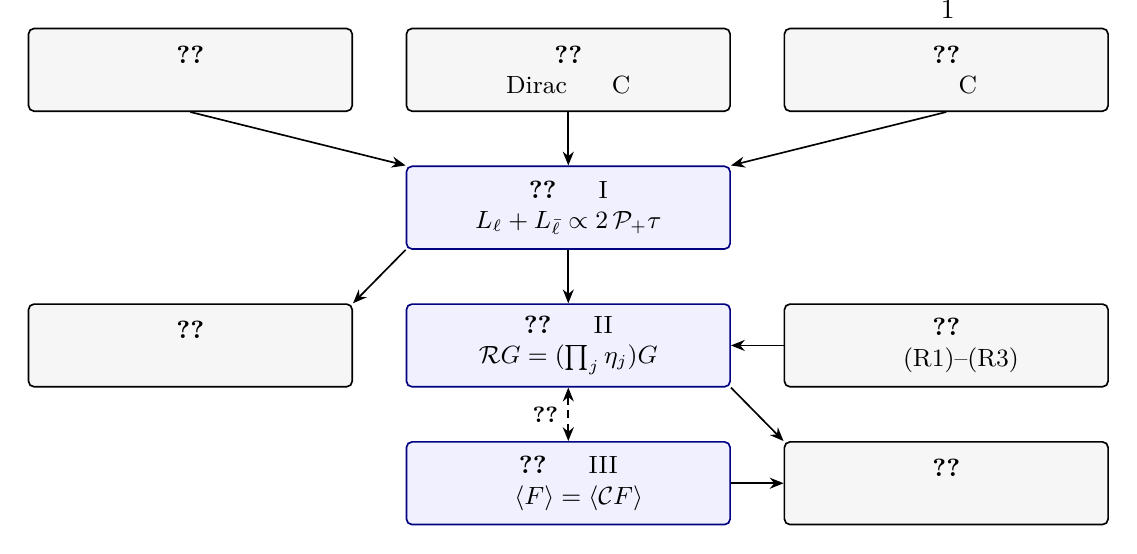
\begin{tikzpicture}[
  blk/.style={draw,rounded corners=2pt,line width=0.6pt,align=flush center,inner sep=3pt,
              font=\small,text width=3.9cm,minimum height=1.05cm},
  thm/.style={blk,fill=blue!6,draw=blue!50!black},
  aux/.style={blk,fill=gray!7},
  dep/.style={-{Stealth[length=5pt,width=4pt]},line width=0.6pt},
  frm/.style={{Stealth[length=5pt,width=4pt]}-{Stealth[length=5pt,width=4pt]},line width=0.6pt,densely dashed}]
\node[aux] (S2) at (-4.8,0)    {\cref{sec:setup}\\ 带标号展开、闭合圈规则};
\node[aux] (S3) at (0,0)       {\cref{sec:dirac}\\ Dirac 空间中的 C};
\node[aux] (S4) at (4.8,0)     {\cref{sec:color}\\ 色空间中的 C};
\node[thm] (S5) at (0,-1.75)   {\cref{sec:thmI}\enspace 主定理 I\\ $L_\ell+L_{\bar\ell}\propto2\,\Pp\tau$};
\node[aux] (S6) at (-4.8,-3.5) {\cref{sec:triangle}\\ 显式例子：三胶子顶点};
\node[thm] (S7) at (0,-3.5)    {\cref{sec:thmII}\enspace 主定理 II\\ $\Rop G=(\prod_j\eta_j)G$};
\node[aux] (S8) at (4.8,-3.5)  {\cref{sec:regularization}\\ 正规化 (R1)--(R3)};
\node[thm] (S9) at (0,-5.25)   {\cref{sec:nonpert}\enspace 主定理 III\\ 格点：$\langle F\rangle=\langle\Cop F\rangle$};
\node[aux] (S10) at (4.8,-5.25){\cref{sec:applications}\\ 物理应用};
\draw[dep] (S2.south) -- (S5.north west);
\draw[dep] (S3.south) -- (S5.north);
\draw[dep] (S4.south) -- (S5.north east);
\draw[dep] (S5.south west) -- (S6.north east);
\draw[dep] (S5.south) -- (S7.north);
\draw[dep] (S8.west) -- (S7.east);
\draw[frm] (S7.south) -- node[left,font=\footnotesize]{\cref{prop:formal}} (S9.north);
\draw[dep] (S9.east) -- (S10.west);
\draw[dep] (S7.south east) -- (S10.north west);
\end{tikzpicture}
\caption{本文的逻辑结构。实线箭头表示证明中的主要依赖（\cref{sec:setup}至\cref{sec:color}的结果也直接用于\cref{sec:thmII}与\cref{sec:nonpert}）；
虚线双箭头表示主定理 II 与主定理 III 之间的关系：连续统中的变量替换（形式地）诱导带标号 Wick 缩并上的对合 $\rho$。}
\label{fig:intro-structure}
\end{figure}

%% ======================================================================
%% 第 2 节  约定、QCD 拉氏量与带标号的微扰展开
%% ======================================================================
\section{约定、QCD 拉氏量与带标号的微扰展开}\label{sec:setup}

本节固定全文的记号与约定，写出规范固定的 QCD 拉氏量与 Feynman 规则，并把微扰展开组织成\emph{顶点带标号}的形式。
这种形式有三个对后文至关重要的特点：
\begin{enumerate}[label=(\roman*),leftmargin=2.2em,itemsep=0pt,topsep=2pt]
\item 对固定的顶点组成 $\nu$（各类顶点的数目，\cref{eq:setup-Nnu}），每个完全 Wick 缩并恰好出现一次，且组合系数都是同一个 $\ii^{|\nu|}/\nu!$，因而从不需要 Feynman 图的对称因子；
\item 每个缩并的值都是“色张量 $\times$ 运动学因子”（或有限个这样的乘积之和）；
\item 夸克场的缩并由置换描述：闭合夸克圈恰为置换的循环，把全部闭合圈同时反向恰为对置换求逆。
\end{enumerate}
\cref{sec:thmI}与\cref{sec:thmII}的 Furry 定理正建立在这三点之上。闭合费米子圈规则（\cref{lem:closed-loops}）的完整证明放在\cref{app:wick}。

%% ----------------------------------------------------------------------
\subsection{记号与约定}\label{sec:setup-notation}

\paragraph{Dirac 矩阵与迹。}
采用自然单位 $\hbar=c=1$ 与度规 $g=\mathrm{diag}(+1,-1,-1,-1)$。Dirac 矩阵满足 $\{\gamma^\mu,\gamma^\nu\}=2g^{\mu\nu}\mathbb 1$，
$\gamma^{\mu\dagger}=\gamma^0\gamma^\mu\gamma^0$，$\bar\psi=\psi^\dagger\gamma^0$；需要具体矩阵时采用 Dirac 表示（\cref{app:dirac}）。定义
\begin{equation}\label{eq:setup-gamma5}
\gamma^5=\ii\gamma^0\gamma^1\gamma^2\gamma^3,\qquad
\sigma^{\mu\nu}=\frac{\ii}{2}\bigl[\gamma^\mu,\gamma^\nu\bigr],\qquad
\sla a=\gamma^\mu a_\mu ,
\end{equation}
则 $(\gamma^5)^2=\mathbb 1$，$\gamma^{5\dagger}=\gamma^5$，$\{\gamma^5,\gamma^\mu\}=0$。$\TrD\mathbb 1=4$；取 $\varepsilon^{0123}=+1$（$\varepsilon_{0123}=-1$），
则 $\TrD(\gamma^5\gamma^\mu\gamma^\nu\gamma^\rho\gamma^\sigma)=-4\ii\,\varepsilon^{\mu\nu\rho\sigma}$。$\Tr$ 表示对所涉矩阵的全部内部指标求迹
（对 Dirac~$\otimes$~色空间上的矩阵为全迹，对色矩阵即为色迹）；需要强调时用 $\TrD$ 与 $\Trc$ 表示只对 Dirac 指标或只对色指标求迹。

\paragraph{传播子与维数正规化。}
质量为 $m$ 的夸克的 Feynman 传播子为
\begin{equation}\label{eq:setup-propagator}
S(p)=\frac{\ii(\sla p+m)}{p^2-m^2+\ii0},\qquad
\SF(x)=\int\!\frac{\dd^4p}{(2\pi)^4}\,\ee^{-\ii p\cdot x}\,S(p),\qquad (\ii\sla\partial-m)\SF(x)=\ii\,\delta^4(x).
\end{equation}
在 $\SF(x-y)$ 中动量 $p$ 沿费米子箭头由 $y$ 流向 $x$。夸克传播子在色空间中是单位矩阵，我们把 $\SF\otimes\mathbb 1_N$ 仍记作 $\SF$。
维数正规化中的时空维数记作 $D=4-2\epsilon$（\cref{def:dimreg-trace}）；带 Lorentz 指标的 $D_\mu$ 与 $D_{\mu\nu}$ 分别表示协变导数与胶子传播子，
闭合圈的 Dirac（运动学）因子则记作 $K_\ell$。

\paragraph{色群。}
规范群为 $\mathrm{SU}(N)$，$N\ge2$（物理情形 $N=3$）。基础表示的生成元 $T^a$（$a=1,\dots,N^2-1$）是无迹 Hermite 矩阵，
\begin{equation}\label{eq:setup-generators}
\Tr\bigl(T^aT^b\bigr)=T_F\,\delta^{ab},\qquad
\bigl[T^a,T^b\bigr]=\ii f^{abc}\,T^c,\qquad
\bigl\{T^a,T^b\bigr\}=\frac1N\,\delta^{ab}\,\mathbb 1+d^{abc}\,T^c ,
\end{equation}
其中 $T_F=\frac12$，$f^{abc}=-2\ii\Tr([T^a,T^b]T^c)$ 实且全反对称，$d^{abc}=2\Tr(\{T^a,T^b\}T^c)$ 实且全对称（实性来自 $T^a$ 的 Hermite 性，
对称性来自迹的循环性）；$\mathrm{SU}(2)$ 中 $d^{abc}\equiv0$。二次 Casimir 为 $T^aT^a=C_F\mathbb 1$，$C_F=(N^2-1)/(2N)$。伴随表示的生成元取
\begin{equation}\label{eq:setup-adjoint}
\bigl(F^a\bigr)_{bc}=-\ii f^{abc},\qquad \bigl[F^a,F^b\bigr]=\ii f^{abc}F^c,\qquad \Tr\bigl(F^aF^b\bigr)=C_A\,\delta^{ab},\quad C_A=N ;
\end{equation}
$F^a$ 是纯虚的反对称 Hermite 矩阵，其对易关系等价于 Jacobi 恒等式（这些标准恒等式见\cite{Haber2021}）。
对 $\mathrm{SU}(3)$ 取 $T^a=\lambda^a/2$（Gell-Mann 矩阵\cite{GellMann1962}），$C_F=4/3$，$C_A=3$；数值表见\cref{app:su3}。

\paragraph{其他约定。}
$\alpha,\beta$ 为 Dirac 指标，$i,j$ 为基础表示色指标，$a,b,c,d,e$ 为伴随指标，$f$ 为味指标（味指标与\cref{sec:setup-expansion}中的味道指派 $\boldsymbol f=(f_1,\dots,f_m)$ 从不带伴随指标，
故不会与 $f^{abc}$ 混淆）；$A,B$ 表示 Dirac~$\otimes$~色复合指标。转置 $X^{\tp}$ 作用于 $X$ 的全部内部指标。沿费米子线书写矩阵乘积时，
矩阵总是\emph{逆着费米子箭头}排列。电荷共轭矩阵 $C$、Clifford 共轭 $\Cconj X:=CX^{\tp}C^{-1}$ 与 C~宇称 $\eta_\Gamma$ 见\cref{lem:C-matrix}与\cref{lem:C-parity}，
色空间中的 $\varphi$、$R$、$\Rop$、$\Pp$、$\Pm$、$\mathcal P_\eta$ 见\cref{def:phi-R}。作为对称性的名称写“C~宇称”“C~偶”“C~奇”（正体），
场空间或 Hilbert 空间上的电荷共轭记作 $\Cop$；Casimir $C_F,C_A$ 总带下标。闭合夸克圈记作 $\ell$，反向圈记作 $\bar\ell$；字母 $c$ 不用来表示圈（作为场它专指鬼场，作为上下标它是伴随指标）。

%% ----------------------------------------------------------------------
\subsection{QCD 拉氏量}\label{sec:setup-lagrangian}

本文研究协变 $\xi$ 规范下、含 $n_f$ 个味道的规范固定 QCD 拉氏量
\begin{equation}\label{eq:lagrangian}
\mathcal L=\sum_{f=1}^{n_f}\bar\psi_f\bigl(\ii\sla D-m_f\bigr)\psi_f-\frac14F^a_{\mu\nu}F^{a\mu\nu}
-\frac{1}{2\xi}\bigl(\partial^\mu A^a_\mu\bigr)^2+\bigl(\partial^\mu\bar c^a\bigr)\bigl(D_\mu c\bigr)^a ,
\end{equation}
\begin{equation}\label{eq:setup-covariant}
\begin{gathered}
D_\mu\psi_f=\bigl(\partial_\mu-\ii gA^a_\mu T^a\bigr)\psi_f,\qquad
\bigl(D_\mu c\bigr)^a=\partial_\mu c^a+gf^{abc}A^b_\mu c^c,\\
F^a_{\mu\nu}=\partial_\mu A^a_\nu-\partial_\nu A^a_\mu+gf^{abc}A^b_\mu A^c_\nu .
\end{gathered}
\end{equation}
这里 $\psi_f$ 是带基础表示色指标的 Grassmann 奇 Dirac 旋量场，质量 $m_f$ 为实数，可以为零；$A^a_\mu$ 是实的胶子场；
$c^a,\bar c^a$ 是伴随表示中彼此独立的 Grassmann 奇标量鬼场（$\bar c$ 不是 $c$ 的共轭）；$\xi$ 为规范参数（Landau 规范 $\xi=0$ 理解为极限）。
质量矩阵是味对角的，各味道互不混合。记 $A_\mu=A^a_\mu T^a$，$F_{\mu\nu}=F^a_{\mu\nu}T^a$，由\cref{eq:setup-generators}，
\begin{equation}\label{eq:setup-Fmatrix}
F_{\mu\nu}=\partial_\mu A_\nu-\partial_\nu A_\mu-\ii g\bigl[A_\mu,A_\nu\bigr]=\frac{\ii}{g}\bigl[D_\mu,D_\nu\bigr],\qquad
-\frac14F^a_{\mu\nu}F^{a\mu\nu}=-\frac12\Tr\bigl(F_{\mu\nu}F^{\mu\nu}\bigr)
\end{equation}
（第一式用到 $-\ii g[A_\mu,A_\nu]=-\ii g\,A^b_\mu A^c_\nu\,\ii f^{bca}T^a=gf^{abc}A^b_\mu A^c_\nu T^a$）。前两项在规范变换
$\psi_f\to U\psi_f$，$A_\mu\to UA_\mu U^{-1}-\tfrac{\ii}{g}(\partial_\mu U)U^{-1}$ 下不变。后两项是规范固定项与 Faddeev--Popov 鬼场项\cite{FaddeevPopov1967}，
后者与 $\bar c^a(-\partial^\mu D_\mu c)^a$ 只差一个全导数\cite[第 16 章]{PeskinSchroeder1995}；它们破坏规范不变性，但保持 BRST 不变性\cite{BRS1976,Tyutin1975}。
各项在电荷共轭下的行为见\cref{prop:L-invariance}。

\paragraph{$\theta$ 项。}
可以在\cref{eq:lagrangian}上加上
\begin{equation}\label{eq:theta-term}
\mathcal L_\theta=\frac{\theta g^2}{32\pi^2}\,F^a_{\mu\nu}\tilde F^{a\mu\nu},\qquad
\tilde F^{a\mu\nu}=\frac12\,\varepsilon^{\mu\nu\rho\sigma}F^a_{\rho\sigma}.
\end{equation}
它是一个全导数：
\begin{equation}\label{eq:setup-chern-simons}
F^a_{\mu\nu}\tilde F^{a\mu\nu}=\partial_\mu J^\mu_{\mathrm{CS}},\qquad
J^\mu_{\mathrm{CS}}=2\,\varepsilon^{\mu\nu\rho\sigma}\Bigl(A^a_\nu\,\partial_\rho A^a_\sigma+\frac g3\,f^{abc}A^a_\nu A^b_\rho A^c_\sigma\Bigr)
\end{equation}
（把\cref{eq:setup-Fmatrix}代入 $F^a_{\mu\nu}\tilde F^{a\mu\nu}=\varepsilon^{\mu\nu\rho\sigma}\Tr(F_{\mu\nu}F_{\rho\sigma})$，用 $\varepsilon^{\mu\nu\rho\sigma}\Tr(A_\mu A_\nu A_\rho A_\sigma)=0$、迹的循环性
以及 $\Tr(T^aT^bT^c)$ 的全反对称部分 $\frac{\ii}{4}f^{abc}$ 直接展开即得；我们也对 $\mathrm{SU}(3)$ 作了符号验证）。
全导数的顶点正比于流入顶点的总动量，由动量守恒而为零，所以 \emph{$\theta$ 项对微扰展开的任何一阶都没有贡献}，只在非微扰层次上起作用。
它破坏 P 与 T（$F^a_{\mu\nu}\tilde F^{a\mu\nu}\propto\boldsymbol E^a\cdot\boldsymbol B^a$），但保持 C（\cref{prop:L-invariance}）。

\paragraph{色单态复合算符。}
我们还考虑味对角的色单态双线性算符
\begin{equation}\label{eq:setup-singlet}
O_j(y)=\sum_{f=1}^{n_f}\kappa_j^{(f)}\,\bar\psi_f(y)\,\Gamma_j\,\psi_f(y)\qquad(\Gamma_j\ \text{为常数 Dirac 矩阵},\ \kappa_j^{(f)}\in\mathbb C),
\end{equation}
例如电磁流 $\sum_fQ_f\bar\psi_f\gamma^\mu\psi_f$、标量密度 $\bar\psi_f\psi_f$、轴矢流 $\bar\psi_f\gamma^\mu\gamma^5\psi_f$。在 QCD$+$QED 中，
光子--夸克顶点 $-\ii eQ_f\gamma^\mu\otimes\mathbb 1$ 也是这样的色单态顶点（\cref{cor:qed}）。

%% ----------------------------------------------------------------------
\subsection{Feynman 规则}\label{sec:setup-feynman}

把\cref{eq:lagrangian}写成 $\mathcal L=\mathcal L_0+\mathcal L_{\mathrm{int}}$，其中 $\mathcal L_0$ 是 $g=0$ 的部分（自由夸克、胶子与鬼场），而
\begin{equation}\label{eq:setup-Lint}
\begin{gathered}
\mathcal L_{\mathrm{int}}=\sum_f\mathcal L^{(f)}_{\mathrm{qg}}+\mathcal L_3+\mathcal L_4+\mathcal L_{\mathrm{gh}},\\
\mathcal L^{(f)}_{\mathrm{qg}}=g\,\bar\psi_f\gamma^\mu T^a\psi_f\,A^a_\mu,\qquad
\mathcal L_{\mathrm{gh}}=g\,f^{abc}\bigl(\partial^\mu\bar c^a\bigr)A^b_\mu\,c^c,\\
\mathcal L_3=-g\,f^{abc}\bigl(\partial_\mu A^a_\nu\bigr)A^{b\mu}A^{c\nu},\qquad
\mathcal L_4=-\frac{g^2}{4}\,f^{eab}f^{ecd}\,A^a_\mu A^b_\nu A^{c\mu}A^{d\nu}.
\end{gathered}
\end{equation}
$\mathcal L^{(f)}_{\mathrm{qg}}$ 来自 $\bar\psi_f\,\ii\gamma^\mu(-\ii gA^a_\mu T^a)\psi_f$；把 $F^a_{\mu\nu}$ 代入 $-\frac14F^aF^a$，交叉项
$-\frac g2f^{abc}(\partial_\mu A^a_\nu-\partial_\nu A^a_\mu)A^{b\mu}A^{c\nu}$ 的两半在 $\mu\leftrightarrow\nu$、$b\leftrightarrow c$ 下相等，给出 $\mathcal L_3$，四次项即 $\mathcal L_4$；
$\mathcal L_{\mathrm{gh}}$ 来自 $(D_\mu c)^a$ 中的 $gf^{abc}A^b_\mu c^c$。$\mathcal L_0$ 给出\cref{fig:feynman-rules}中的传播子（例如胶子二次型
$-k^2g_{\mu\nu}+(1-\xi^{-1})k_\mu k_\nu$ 的逆乘以 $\ii$ 即胶子传播子）。顶点规则等于 $\ii$ 乘以相应单项式的系数，对外腿与单项式中各场的一切指派求和，
并把作用在携带流入动量 $p$ 的场（平面波因子 $\ee^{-\ii p\cdot x}$）上的 $\partial_\mu$ 换成 $-\ii p_\mu$：夸克--胶子顶点给出 $\ii g\gamma^\mu T^a$；
鬼场--胶子顶点中导数作用于 $\bar c^a$，其鬼场线以动量 $p$ 沿箭头\emph{离开}顶点，故 $\partial^\mu\to+\ii p^\mu$，顶点为 $\ii\cdot gf^{abc}\cdot\ii p^\mu=-gf^{abc}p^\mu$；
三、四胶子顶点分别是 $3!$、$4!$ 种指派之和。这些规则与\cite[第 16 章]{PeskinSchroeder1995}一致（我们也用计算机核对了对指派的求和，
并用符号计算验证了 $\mathcal L_3$、$\mathcal L_4$ 的推导）；闭合圈的规则（因子 $-1$ 与求迹）在\cref{sec:setup-loops}中给出。

%% ---------------------------------------------------------------- figure
\begin{figure}[htbp]
\centering
\small
\setlength{\tabcolsep}{6pt}
\begin{tabular}{@{}cl@{}}
\toprule
Feynman 图 & 表达式 \\
\midrule
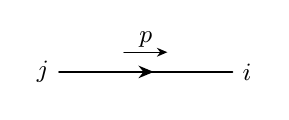
\begin{tikzpicture}[fd,baseline={([yshift=-.5ex]current bounding box.center)}]
  \draw[quark] (0,0) node[left]{$j$} -- (2.2,0) node[right]{$i$};
  \path[mom={$p$}] (0,0) -- (2.2,0);
\end{tikzpicture}
&
\begin{tabular}[c]{@{}l@{}}
{\footnotesize 夸克传播子}\\[2pt]
$\displaystyle \frac{\ii(\slashed{p}+m)}{p^2-m^2+\ii0}\,\delta_{ij}$
\end{tabular}
\\ \addlinespace[8pt]
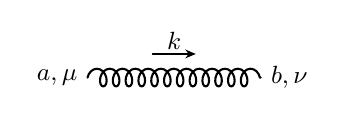
\begin{tikzpicture}[fd,baseline={([yshift=-.5ex]current bounding box.center)}]
  \draw[gluon] (0,0) node[left]{$a,\mu$} -- (2.2,0) node[right]{$b,\nu$};
  \path[mom sep=0.3cm,mom={$k$}] (0,0) -- (2.2,0);
\end{tikzpicture}
&
\begin{tabular}[c]{@{}l@{}}
{\footnotesize 胶子传播子（协变规范，规范参数 $\xi$）}\\[2pt]
$\displaystyle \frac{-\ii\,\delta^{ab}}{k^2+\ii0}\Big[g^{\mu\nu}-(1-\xi)\frac{k^\mu k^\nu}{k^2}\Big]$
\end{tabular}
\\ \addlinespace[8pt]
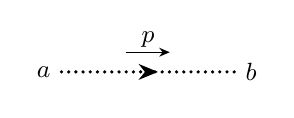
\begin{tikzpicture}[fd,baseline={([yshift=-.5ex]current bounding box.center)}]
  \draw[ghost] (0,0) node[left]{$a$} -- (2.2,0) node[right]{$b$};
  \path[mom={$p$}] (0,0) -- (2.2,0);
\end{tikzpicture}
&
\begin{tabular}[c]{@{}l@{}}
{\footnotesize 鬼场传播子}\\[2pt]
$\displaystyle \frac{\ii\,\delta^{ab}}{p^2+\ii0}$
\end{tabular}
\\ \addlinespace[8pt]
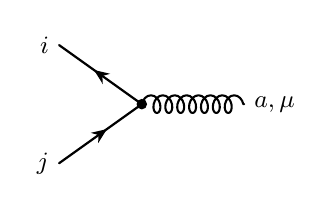
\begin{tikzpicture}[fd,baseline={([yshift=-.5ex]current bounding box.center)}]
  \coordinate (v) at (0,0);
  \draw[quark] (-1.05,-0.75) node[left]{$j$} -- (v);
  \draw[quark] (v) -- (-1.05,0.75) node[left]{$i$};
  \draw[gluon] (v) -- (1.3,0) node[right]{$a,\mu$};
  \node[vertex] at (v) {};
\end{tikzpicture}
&
\begin{tabular}[c]{@{}l@{}}
{\footnotesize 夸克--胶子顶点}\\[2pt]
$\displaystyle \ii g\,\gamma^\mu\,(T^a)_{ij}$
\end{tabular}
\\ \addlinespace[8pt]
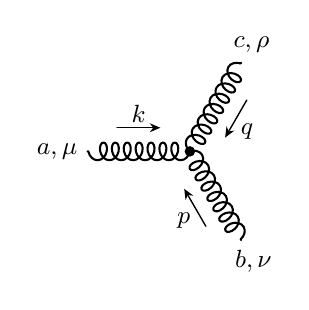
\begin{tikzpicture}[fd,baseline={([yshift=-.5ex]current bounding box.center)}]
  \coordinate (v) at (0,0);
  \draw[gluon] (v) -- (180:1.3) coordinate (ea) node[left]{$a,\mu$};
  \draw[gluon] (v) -- (-60:1.3) coordinate (eb) node[anchor=120]{$b,\nu$};
  \draw[gluon] (v) -- (60:1.3) coordinate (ec) node[anchor=-120]{$c,\rho$};
  \path[mom sep=0.3cm,mom={$k$}] (ea) -- (v);
  \path[mom sep=0.3cm,mom={$p$}] (eb) -- (v);
  \path[mom sep=0.3cm,mom={$q$}] (ec) -- (v);
  \node[vertex] at (v) {};
\end{tikzpicture}
&
\begin{tabular}[c]{@{}l@{}}
{\footnotesize 三胶子顶点（动量 $k,p,q$ 全部流入顶点）}\\[2pt]
$\displaystyle g f^{abc}\big[g^{\mu\nu}(k-p)^\rho+g^{\nu\rho}(p-q)^\mu+g^{\rho\mu}(q-k)^\nu\big]$
\end{tabular}
\\ \addlinespace[8pt]
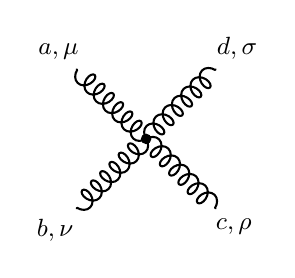
\begin{tikzpicture}[fd,baseline={([yshift=-.5ex]current bounding box.center)}]
  \coordinate (v) at (0,0);
  \draw[gluon] (v) -- (135:1.25) node[anchor=-45]{$a,\mu$};
  \draw[gluon] (v) -- (225:1.25) node[anchor=45]{$b,\nu$};
  \draw[gluon] (v) -- (315:1.25) node[anchor=135]{$c,\rho$};
  \draw[gluon] (v) -- (45:1.25) node[anchor=-135]{$d,\sigma$};
  \node[vertex] at (v) {};
\end{tikzpicture}
&
\begin{tabular}[c]{@{}l@{}}
{\footnotesize 四胶子顶点}\\[2pt]
$\displaystyle \begin{aligned}[t]
-\ii g^2\big[&f^{abe}f^{cde}(g^{\mu\rho}g^{\nu\sigma}-g^{\mu\sigma}g^{\nu\rho})\\
&+f^{ace}f^{bde}(g^{\mu\nu}g^{\rho\sigma}-g^{\mu\sigma}g^{\nu\rho})\\
&+f^{ade}f^{bce}(g^{\mu\nu}g^{\rho\sigma}-g^{\mu\rho}g^{\nu\sigma})\big]
\end{aligned}$
\end{tabular}
\\ \addlinespace[8pt]
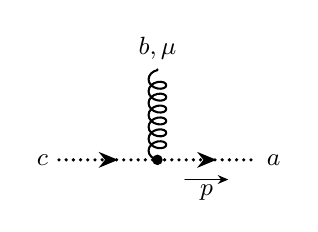
\begin{tikzpicture}[fd,baseline={([yshift=-.5ex]current bounding box.center)}]
  \coordinate (v) at (0,0);
  \draw[ghost] (-1.25,0) node[left]{$c$} -- (v);
  \draw[ghost] (v) -- (1.25,0) node[right]{$a$};
  \draw[gluon] (v) -- (0,1.15) node[above]{$b,\mu$};
  \path[mom'={$p$}] (v) -- (1.25,0);
  \node[vertex] at (v) {};
\end{tikzpicture}
&
\begin{tabular}[c]{@{}l@{}}
{\footnotesize 鬼场--胶子顶点（$a$：出射鬼场，动量 $p$ 流出；$c$：入射鬼场）}\\[2pt]
$\displaystyle -g f^{abc}\,p^\mu$
\end{tabular}
\\ \addlinespace[8pt]
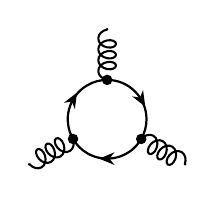
\begin{tikzpicture}[fd,baseline={([yshift=-.5ex]current bounding box.center)}]
  \draw[quark] (90:0.5) arc[start angle=90,end angle=-30,radius=0.5];
  \draw[quark] (-30:0.5) arc[start angle=-30,end angle=-150,radius=0.5];
  \draw[quark] (210:0.5) arc[start angle=210,end angle=90,radius=0.5];
  \foreach \ang in {90,210,330}{
    \draw[gluon] (\ang:0.5) -- (\ang:1.15);
    \node[vertex] at (\ang:0.5) {};}
\end{tikzpicture}
&
\begin{tabular}[c]{@{}l@{}}
{\footnotesize 闭合费米子圈（\cref{lem:closed-loops}）}\\[2pt]
每个闭合夸克圈：因子 $(-1)$，并对 Dirac 指标与色指标求迹；\\
每个闭合鬼场圈：同样给出因子 $(-1)$，色因子 $\propto$ 伴随表示中的迹。
\end{tabular}
\\
\bottomrule
\end{tabular}
\caption{QCD 的 Feynman 规则（Peskin--Schroeder 约定，$D_\mu=\partial_\mu-\ii gA^a_\mu T^a$，协变规范）。
夸克传播子中动量 $p$ 沿费米子箭头方向，色指标由 $j$ 流向 $i$；夸克--胶子顶点 $(T^a)_{ij}$ 中的 $i$ 属于沿箭头离开顶点的夸克线；
三胶子顶点的动量 $k,p,q$ 全部流入顶点；$\ii0$ 表示 Feynman 的无穷小虚部规定。}
\label{fig:feynman-rules}
\end{figure}

\paragraph{色--运动学分解。}
除四胶子顶点外，\cref{fig:feynman-rules}中的每条传播子与每个顶点都是“色张量 $\times$ 不带色指标的运动学因子”：$\delta_{ij}\times S(p)$，$\delta^{ab}\times D_{\mu\nu}(k)$，
$\delta^{ab}\times\ii/(p^2+\ii0)$，$(T^a)_{ij}\times\ii g\gamma^\mu$，三胶子顶点与鬼场--胶子顶点 $f^{abc}\times(\cdots)$，色单态插入 $\mathbb 1\times\kappa\Gamma$。
四胶子顶点则是三个这样的乘积之和：
\begin{equation}\label{eq:setup-4g}
V_4=\sum_{s=1}^{3}C^{(s)}K^{(s)},\qquad
C^{(1)}=f^{abe}f^{cde},\quad C^{(2)}=f^{ace}f^{bde},\quad C^{(3)}=f^{ade}f^{bce},
\end{equation}
$K^{(s)}$ 是\cref{fig:feynman-rules}中相应的 Lorentz 张量，例如 $K^{(1)}=-\ii g^2(g^{\mu\rho}g^{\nu\sigma}-g^{\mu\sigma}g^{\nu\rho})$。
色指标只通过传播子的 $\delta$ 与色指标缩并，Lorentz 指标与时空坐标只出现在运动学因子中；这是\cref{lem:setup-factorization}的基础。

%% ----------------------------------------------------------------------
\subsection{Green 函数与带标号的微扰展开}\label{sec:setup-expansion}

\paragraph{Green 函数及其微扰定义。}
设
\begin{equation}\label{eq:setup-Phiext}
\Phi_{\mathrm{ext}}=\prod_{i=1}^{n_A}A^{a_i}_{\mu_i}(x_i)\,\prod_{i=1}^{n_c}c^{b_i}(x'_i)\,\prod_{i=1}^{n_{\bar c}}\bar c^{\,\bar b_i}(x''_i)\,\prod_{j=1}^{m}O_j(y_j),
\end{equation}
完全 Green 函数 $G=\langle\Omega|\mathrm T\,\Phi_{\mathrm{ext}}|\Omega\rangle$ 是带 $n_A+n_c+n_{\bar c}$ 个伴随指标的色张量，其分量还依赖于 Lorentz 指标与坐标
（或动量）。含外夸克场的 Green 函数（其缩并中有开放的夸克线）不在本文主要定理的范围之内。在微扰论中，
\begin{equation}\label{eq:setup-GML}
G=\frac{\mathcal N}{\mathcal Z},\qquad
\mathcal N=\Bigl\langle\Phi_{\mathrm{ext}}\exp\Bigl(\ii\!\int\!\dd^4z\,\mathcal L_{\mathrm{int}}(z)\Bigr)\Bigr\rangle_0,\qquad
\mathcal Z=\Bigl\langle\exp\Bigl(\ii\!\int\!\dd^4z\,\mathcal L_{\mathrm{int}}(z)\Bigr)\Bigr\rangle_0 ,
\end{equation}
其中 $\langle X\rangle_0:=\langle0|\mathrm T\,X|0\rangle_0$ 是自由理论 $\mathcal L_0$ 中的编时真空期望值。这在算符形式中就是 Gell-Mann--Low 公式
（导数耦合须用协变的 $\mathrm T^*$ 乘积），在泛函积分中则由展开 $\ee^{\ii S_{\mathrm{int}}}$ 得到；由泛函积分导出的 QCD Feynman 规则见\cite[第 16 章]{PeskinSchroeder1995}。
本文\emph{以\cref{eq:setup-GML}（$\langle\cdots\rangle_0$ 按下述 Wick 定理计算）作为微扰 Green 函数的定义}（无穷体积时的含义见\cref{lem:setup-vacuum}的证明）：$G$ 是 $g$ 的形式幂级数，
每个系数是有限个积分之和。后文把 $\ell$ 与 $\bar\ell$ 联系起来的关系在坐标空间中都是被积函数之间的恒等式，对固定的顶点位置逐点成立；
在动量空间中，互为反向的圈须采用镜像动量配置（\cref{sec:setup-loops}“取向的含义”一段之末，\cref{fig:dirac-mirror}）才逐点成立，
而顶点 C~宇称之积为 $-1$ 的自反向短圈（长度 $\le2$）所需的 $K_\ell=0$ 只在积分之后成立（\cref{rem:reg-selfreverse}）。
在\cref{def:reg-hypotheses}的条件下，这些关系对正规化后的积分都成立（坐标空间中只需 (R1)，但正规化传播子须在顶点重合处也有定义；动量空间中还需 (R2)；见\cref{sec:reg-rigour}）。

\paragraph{自由两点函数。}
$\mathcal L_0$ 给出
\begin{equation}\label{eq:setup-free}
\begin{gathered}
\bigl\langle A^a_\mu(x)A^b_\nu(y)\bigr\rangle_0=\delta^{ab}D_{\mu\nu}(x-y),\qquad
\bigl\langle c^a(x)\bar c^b(y)\bigr\rangle_0=\delta^{ab}\Delta_0(x-y),\\
\bigl\langle\psi_{f\alpha i}(x)\bar\psi_{f'\beta j}(y)\bigr\rangle_0=\delta_{ff'}\,\delta_{ij}\,\SF^{(f)}(x-y)_{\alpha\beta},
\end{gathered}
\end{equation}
其中 $\SF^{(f)}$ 是\cref{eq:setup-propagator}中取 $m=m_f$ 的 $\SF$，而 $D_{\mu\nu}$ 与 $\Delta_0$ 分别是\cref{fig:feynman-rules}中胶子与鬼场传播子（去掉 $\delta^{ab}$）
按\cref{eq:setup-propagator}的约定所作的 Fourier 变换；
其余的两点函数（$\langle\psi\psi\rangle_0$、$\langle\bar\psi\bar\psi\rangle_0$、$\langle cc\rangle_0$、$\langle\bar c\bar c\rangle_0$ 及不同场之间的两点函数）为零。
导数总取在期望值之外，例如 $\langle\partial_\kappa A(x)\,A(y)\rangle_0=\partial^x_\kappa\langle A(x)A(y)\rangle_0$。

\paragraph{带标号的展开。}
$\mathcal L^{(f)}_{\mathrm{qg}}$、$\mathcal L_3$、$\mathcal L_4$、$\mathcal L_{\mathrm{gh}}$ 都是 Grassmann 偶的，在编时乘积中彼此对易，故由多项式定理，
\begin{equation}\label{eq:setup-Nnu}
\begin{gathered}
\mathcal N=\sum_{\nu}\mathcal N_\nu,\qquad
\mathcal N_\nu=\frac{\ii^{|\nu|}}{\nu!}\int\!\dd\mu_\nu\,\bigl\langle\Phi_{\mathrm{ext}}\,\mathcal I_\nu\bigr\rangle_0,\\
\mathcal I_\nu=\prod_{f}\prod_{j=1}^{n^{(f)}_q}\mathcal L^{(f)}_{\mathrm{qg}}\bigl(z^{(f)}_j\bigr)\,\prod_{l=1}^{n_3}\mathcal L_3(u_l)\,\prod_{r=1}^{n_4}\mathcal L_4(v_r)\,\prod_{s=1}^{n_{\mathrm{gh}}}\mathcal L_{\mathrm{gh}}(w_s),
\end{gathered}
\end{equation}
其中 $\nu=\bigl(n^{(1)}_q,\dots,n^{(n_f)}_q;n_3,n_4,n_{\mathrm{gh}}\bigr)$ 遍历非负整数组，$|\nu|=\sum_fn^{(f)}_q+n_3+n_4+n_{\mathrm{gh}}$，
$\nu!=\prod_fn^{(f)}_q!\cdot n_3!\,n_4!\,n_{\mathrm{gh}}!$，$\dd\mu_\nu$ 是对全部顶点位置的积分测度；$\mathcal N_\nu\propto g^{|\nu|+n_4}$。
各类顶点按 $j,l,r,s$ 编号，并且每个单项式中的各个场也视为可区分的“槽位”（例如 $\mathcal L_4$ 的四个胶子场）——这就是\emph{带标号的}展开。

\paragraph{Wick 定理。}
自由测度是胶子、各味道夸克与鬼场的 Gauss 测度之积，而夸克双线性型与胶子场是 Grassmann 偶的，可以移到鬼场之外而不产生符号；
因此\cref{eq:setup-Nnu}中的期望值（提出常数系数后）分解为胶子、各味道夸克与鬼场三部分之积，它们分别按如下规则计算：
(a) 胶子：对全部胶子槽位（外胶子场与各单项式中的胶子场）的完美配对 $P$ 求和，每一对贡献一个两点函数（\cref{lem:app-wick-boson}）；
(b) 夸克场：按\cref{eq:app-wick-continuum}的行列式规则计算（不同味道之间的两点函数为零）；对味道 $f$ 的双线性型之积，
其期望值化为对这些双线性型的置换 $\pi_f$ 的求和（\cref{lem:closed-loops}，由此规则推出，见\cref{app:wick-proof}）；
(c) 鬼场：对由 $c$-槽位到 $\bar c$-槽位的双射 $\sigma$ 求和，每项带 Grassmann 重排的符号 $\operatorname{sgn}_{\mathrm{gh}}(\sigma)\in\{\pm1\}$（\cref{prop:app-wick-det}），
不含外鬼场时 $\operatorname{sgn}_{\mathrm{gh}}(\sigma)=(-1)^{\#\mathrm{cyc}(\sigma)}$（\cref{app:wick-ghost}）。
外插入 $O_j$ 带有味道求和，按多线性展开为对味道指派 $\boldsymbol f=(f_1,\dots,f_m)$ 的求和：$\prod_jO_j=\sum_{\boldsymbol f}\prod_j\kappa_j^{(f_j)}\bar\psi_{f_j}\Gamma_j\psi_{f_j}$；
对固定的 $\boldsymbol f$，味道 $f$ 的双线性型是 $n^{(f)}_q$ 个夸克--胶子顶点与 $f_j=f$ 的那些插入。

\begin{definition}[完全 Wick 缩并]\label{def:setup-contraction}
固定 $\nu$ 与插入的味道指派 $\boldsymbol f$。一个\emph{完全 Wick 缩并}是 $W=\bigl(P,(\pi_f)_{f},\sigma\bigr)$，其中 $P$ 是全部胶子槽位的一个完美配对；
$\pi_f$ 是味道 $f$ 的双线性型集合上的置换（第 $i$ 个双线性型中的 $\psi_f$ 与第 $\pi_f(i)$ 个中的 $\bar\psi_f$ 缩并）；
$\sigma$ 是 $c$-槽位集合到 $\bar c$-槽位集合的双射（槽位 $t$ 中的 $c$ 与槽位 $\sigma(t)$ 中的 $\bar c$ 缩并）。全体完全 Wick 缩并构成有限集合 $\mathcal W_\nu$（它也依赖于 $\boldsymbol f$，记号中略去）。
$W$ 的\emph{值} $\operatorname{val}(W)$ 是 $\ii^{|\nu|}/\nu!$ 乘以：按 $W$ 把 $\Phi_{\mathrm{ext}}\mathcal I_\nu$ 中的全部场换成两点函数所得的被积函数
（带上符号 $\operatorname{sgn}_{\mathrm{gh}}(\sigma)$ 与每个闭合夸克圈的因子 $-1$），再对全部顶点位置积分。于是
\begin{equation}\label{eq:setup-sum}
\mathcal N=\sum_\nu\sum_{\boldsymbol f}\sum_{W\in\mathcal W_\nu}\operatorname{val}(W).
\end{equation}
\end{definition}

由\cref{lem:closed-loops}，$\operatorname{val}(W)$ 中味道 $f$ 的夸克部分为 $\prod_{\ell\in\mathrm{cyc}(\pi_f)}L_\ell$，每个闭合圈只带一个味道。
由于 $\pi_f$ 是置换，\emph{每个夸克--胶子顶点与每个色单态插入都恰好位于一个闭合夸克圈上}。

\begin{lemma}[色--运动学分解]\label{lem:setup-factorization}
对每个 $W\in\mathcal W_\nu$，存在有限和
\begin{equation}\label{eq:setup-value}
\operatorname{val}(W)=\sum_{s}C_s(W)\,K_s(W),
\end{equation}
使得：(i) $C_s(W)$ 是色张量，其自由指标恰为外胶子场、外鬼场与外反鬼场的伴随指标；它是以下色张量沿 $P$ 与 $\sigma$（每一对贡献一个 $\delta$）的完全缩并：
三胶子顶点与鬼场--胶子顶点的 $f^{abc}$，四胶子顶点的色结构（由 $s$ 选定），以及每个闭合夸克圈 $\ell=(i_1\cdots i_k)$ 的色迹
$\Tr(M_{i_1}\cdots M_{i_k})$（夸克--胶子顶点 $M=T^a$，色单态插入 $M=\mathbb 1$）。(ii) $K_s(W)$ 不依赖于任何色指标，它是以下因子之积对顶点位置的积分：
$1/\nu!$；胶子与鬼场传播子；三胶子、四胶子与鬼场--胶子顶点的 Lorentz 部分，各连同其耦合常数与来自 $\ii^{|\nu|}$ 的一个因子 $\ii$；每个闭合夸克圈的因子
$-\bigl(\prod_j\kappa_{i_j}\bigr)K_\ell$（\cref{eq:loop-factorized}；夸克--胶子顶点的 $\kappa=\ii g$ 已含其因子 $\ii$，插入 $O_j$ 的 $\kappa$ 即味道权重 $\kappa_j^{(f_j)}$）；$\operatorname{sgn}_{\mathrm{gh}}(\sigma)$。
换言之，$\ii^{|\nu|}$ 的每个因子 $\ii$ 都已按 Feynman 规则并入相应的相互作用顶点。
(iii) 把各闭合圈的色迹看作其顶点上伴随指标的张量，则这些张量与其余色张量的缩并方式只依赖于 $P$、$\sigma$ 与各闭合圈上的顶点集合，
不依赖于圈的取向（取向只改变色迹本身，见\cref{eq:setup-reversed}）。
（关于\cref{eq:setup-value}中对 $s$ 的求和：按\cref{eq:setup-Lint}原样使用单项式时只有一项；若把 $\mathcal L_4$ 写成其四个场的 $4!$ 种排列的平均，则每个四胶子顶点因子为 $V_4/4!$，
$s\in\{1,2,3\}^{n_4}$ 选定各四胶子顶点所取的\cref{eq:setup-4g}中的项。）
\end{lemma}

\begin{proof}
把 $\ii^{|\nu|}$ 的 $|\nu|$ 个因子 $\ii$ 逐个分给相互作用顶点，则 $\ii^{|\nu|}$ 乘以被积函数是以下因子之积：
胶子与鬼场两点函数 $\delta^{ab}D_{\mu\nu}$、$\delta^{ab}\Delta_0$（或其导数），三胶子、四胶子与鬼场--胶子顶点的系数（乘以 $\ii$），
$\operatorname{sgn}_{\mathrm{gh}}(\sigma)$，以及各闭合夸克圈的 $L_\ell$（其中夸克--胶子顶点取 $V=\ii g\gamma^\mu\otimes T^a$，插入 $O_j$ 取 $V=\kappa_j^{(f_j)}\Gamma_j\otimes\mathbb 1$）。除 $L_\ell$ 外，每个因子都是一个色张量（$\delta^{ab}$、$f^{abc}$ 或 $f^{abe}f^{cde}$ 型）与一个不带色指标的因子之积，
导数只作用于后者；对平均后的 $\mathcal L_4$，顶点因子是 $V_4/4!$（$V_4$ 正是 $\ii$ 乘以对 $4!$ 种指派的求和），即三个这样的乘积之和。
对 $L_\ell$ 用\cref{eq:loop-factorized}。色指标只通过 $\delta$ 与色指标缩并，Lorentz 指标与坐标只出现在不带色指标的因子中，展开乘积即得\cref{eq:setup-value}。
(iii) 成立，因为 $\ell$ 与 $\bar\ell$ 由同一组顶点组成，其色迹是这些顶点上胶子指标的张量，而这些指标与网络其余部分的连接由 $P$ 决定。
\end{proof}

\begin{lemma}[真空归一化]\label{lem:setup-vacuum}
在有限时空体积中（顶点位置限制在有限区域内），$\mathcal Z$ 是常数项为 $1$、不带任何外指标的形式幂级数。以上标 ${}^{(r)}$ 表示 $g^r$ 的系数，则
\begin{equation}\label{eq:setup-vacuum}
G^{(r)}=\sum_{t=0}^{r}\mathcal N^{(t)}\,\bigl(\mathcal Z^{-1}\bigr)^{(r-t)} .
\end{equation}
特别地，若线性映射 $\mathfrak L$ 只作用于外色指标（例如\cref{def:phi-R}中的 $\Rop$），且对一切 $t$ 有 $\mathfrak L\mathcal N^{(t)}=\eta\,\mathcal N^{(t)}$（$\eta$ 与 $t$ 无关），
则对一切 $r$ 有 $\mathfrak L\,G^{(r)}=\eta\,G^{(r)}$。
\end{lemma}

\begin{proof}
$\mathcal Z$ 是\cref{eq:setup-sum}在 $\Phi_{\mathrm{ext}}=1$ 时的特例，其 $\nu=0$ 项为 $1$，故可逆；\cref{eq:setup-vacuum}即 $G=\mathcal N\mathcal Z^{-1}$ 的逐阶形式，
而 $(\mathcal Z^{-1})^{(r-t)}$ 不带外指标，与 $\mathfrak L$ 对易。

无穷体积中 $\mathcal Z$ 的系数含体积发散；此时 $G^{(r)}$ 是在有限体积中按\cref{eq:setup-vacuum}算出的值在区域趋于全空间时的极限，
$\mathfrak L$ 是固定的有限维线性映射，与取极限交换。等价地，称缩并中不含外场的连通分量为真空分量，记 $G_{\mathrm{nv}}$ 为不含真空分量的缩并之和：
带标号顶点在含外场分量与真空分量之间的分配方式数恰好把组合系数 $\ii^{|\nu|}/\nu!$ 化为两部分各自的组合系数之积，闭合圈的因子 $-1$ 与 $\operatorname{sgn}_{\mathrm{gh}}$ 也按分量分解，
故逐阶 $\mathcal N=G_{\mathrm{nv}}\mathcal Z$，即 $G=G_{\mathrm{nv}}$。这一刻画不需要有限体积，也适用于动量空间中的维数正规化；
而不含真空分量的缩并的集合在\cref{def:rho}的对合 $\rho$ 下封闭，故取 $\mathfrak L=\Rop$ 时所需的结论可直接对 $G_{\mathrm{nv}}$ 得到（\cref{thm:furry-allorders}证明的第二步）。
\end{proof}

连通、截腿与单粒子不可约 Green 函数的处理见\cref{thm:furry-allorders}证明的第三至五步。

\begin{remark}[带标号的顶点与对称因子]\label{rem:setup-symmetry}
对固定的 $\nu$，每个 $W\in\mathcal W_\nu$ 恰好出现一次，且组合系数都是 $\ii^{|\nu|}/\nu!$。通常的无标号 Feynman 图对应于 $\mathcal W_\nu$ 在重新编号
（同类顶点的置换与单项式内同类场的置换）作用下的轨道，把一个轨道内的缩并合并起来才会产生对称因子。本文的论证（\cref{thm:furry-allorders}的证明）只用到\cref{def:rho}中的对合 $\rho$（\cref{prop:formal}中的变量替换在微扰展开中诱导的正是 $\rho$），
它是 $\mathcal W_\nu$ 上的双射，因而\emph{只涉及带标号的缩并，从不需要对称因子}。在圈反向下映为自身的无标号图（“自共轭图”）见\cref{rem:thmII-selfconj}。
\end{remark}

\begin{remark}[抵消项]\label{rem:setup-counterterms}
重整化微扰论中 $\mathcal L_{\mathrm{int}}$ 还含有抵消项。在维数正规化与 $\overline{\mathrm{MS}}$ 方案中（\cref{prop:reg-dimreg}），它们与 $\mathcal L_0$ 及\cref{eq:setup-Lint}的各项有相同的场内容与色结构，
只是乘以重整化常数的展开系数；其他正规化可能需要别的局域抵消项，它们须满足\cref{def:reg-hypotheses}的 (R3)（另见\cref{rem:thmII-general-vertices}）。
在带标号的展开中，抵消项都只是另外几种顶点，上述论述不变。含导数的夸克两点抵消项 $\bar\psi_f(\ii\delta_2\sla\partial-\delta_m)\psi_f$ 在闭合圈中的处理由\cref{prop:app-wick-cycles}覆盖。
抵消项的 C~性质见\cref{lem:building-blocks}与\cref{prop:reg-dimreg}。
\end{remark}

%% ----------------------------------------------------------------------
\subsection{闭合费米子圈与圈的取向}\label{sec:setup-loops}

对每个味道，夸克部分的自由期望值由下面的引理给出。

\begin{lemma}[闭合费米子圈规则]\label{lem:closed-loops}
设 $V_1,\dots,V_K$ 为作用于 Dirac~$\otimes$~色空间的常数矩阵（可带 Lorentz 指标），
$\psi$ 为单一味道的自由夸克场，$\SF(x-y)=\langle0|\mathrm T\,\psi(x)\bar\psi(y)|0\rangle_0$。则
\begin{equation}\label{eq:closed-loops}
\Bigl\langle0\Bigm|\mathrm T\prod_{i=1}^{K}\bar\psi(z_i)V_i\psi(z_i)\Bigm|0\Bigr\rangle_0
=\sum_{\pi\in S_K}\ \prod_{\ell\in\mathrm{cyc}(\pi)}L_\ell ,
\end{equation}
其中 $\mathrm{cyc}(\pi)$ 为置换 $\pi$ 的循环分解；对循环 $\ell=(i_1\,i_2\,\cdots\,i_k)$（即 $\pi(i_j)=i_{j+1}$，下标模 $k$），
\begin{equation}\label{eq:loop-factor}
L_\ell=-\Tr\Bigl[V_{i_1}\SF(z_{i_1}-z_{i_2})\,V_{i_2}\SF(z_{i_2}-z_{i_3})\cdots V_{i_k}\SF(z_{i_k}-z_{i_1})\Bigr],
\end{equation}
迹同时取遍 Dirac 指标与色指标。这里 $\psi(z_{i_j})$ 与 $\bar\psi(z_{i_{j+1}})$ 缩并，费米子数沿
$z_{i_{j+1}}\to z_{i_j}$ 的方向流动，矩阵按逆着费米子箭头的次序书写；每个闭合圈的因子 $-1$ 与圈的取向无关。
（若顶点按正规乘积定义，则长度为 $1$ 的循环不出现。）
\end{lemma}

证明见\cref{app:wick}：把每个双线性型写成 $\bar\psi V\psi=-V_{AB}\,\psi_B\bar\psi_A$，用 Grassmann--Gauss 积分的行列式公式（\cref{prop:app-wick-det}）按置换展开，再用
\begin{equation}\label{eq:setup-sign}
(-1)^K\operatorname{sgn}\pi=(-1)^{\#\mathrm{cyc}(\pi)}
\end{equation}
（长度为 $k$ 的循环是 $k-1$ 个对换之积）。
长度为 $1$ 的循环（“蝌蚪”）含 $\SF(0)$，其值由正规化给出；对夸克--胶子顶点它因 $\Tr T^a=0$ 而为零，对正规乘积的顶点它不出现（\cref{app:wick-normal}）。
\cref{app:wick-cycles}还把引理推广到任意双线性核（例如含导数的抵消项顶点与鬼场顶点）。

在 QCD 中，顶点是“耦合常数 $\times$ Dirac 矩阵 $\otimes$ 色矩阵”，于是圈因子分解为 Dirac 部分与色部分。

\begin{definition}[圈因子的分解与反向圈]\label{def:loop-factor}
设顶点为 $V_i=\kappa_i\,\Gamma_i\otimes M_i$，其中 $\kappa_i\in\mathbb C$ 为耦合常数，$\Gamma_i$ 为 Dirac 矩阵，
$M_i$ 为色空间矩阵（夸克--胶子顶点：$\kappa=\ii g$，$\Gamma=\gamma^\mu$，$M=T^a$；味对角的色单态顶点：$M=\mathbb 1$）。
由于 $\SF$ 在色空间中正比于单位矩阵，
\begin{equation}\label{eq:loop-factorized}
\begin{gathered}
L_\ell=-\Bigl(\prod_{j=1}^{k}\kappa_{i_j}\Bigr)\,K_\ell\,\Tr\bigl(M_{i_1}M_{i_2}\cdots M_{i_k}\bigr),\\
K_\ell=\TrD\Bigl[\Gamma_{i_1}\SF(z_{i_1}-z_{i_2})\,\Gamma_{i_2}\SF(z_{i_2}-z_{i_3})\cdots\Gamma_{i_k}\SF(z_{i_k}-z_{i_1})\Bigr].
\end{gathered}
\end{equation}
对只含夸克--胶子顶点的圈，记其色迹为 $\tau_\ell=\Tr\bigl(T^{a_{i_1}}T^{a_{i_2}}\cdots T^{a_{i_k}}\bigr)$。
圈 $\ell$ 的反向圈定义为 $\bar\ell=(i_1\,i_k\,i_{k-1}\,\cdots\,i_2)$；当 $k\ge3$ 时 $\bar\ell\neq\ell$，当 $k\le2$ 时 $\bar\ell=\ell$。
把置换 $\pi$ 的全部循环同时反向，恰好得到 $\pi^{-1}$。
\end{definition}

\cref{eq:loop-factorized}只用到 $(A\otimes B)(A'\otimes B')=AA'\otimes BB'$ 与 $\Tr(A\otimes B)=\TrD A\cdot\Trc B$。定义中关于反向圈的断言证明如下。

\begin{proof}[定义中断言的证明]
把 $\ell$ 看作其支撑 $\{i_1,\dots,i_k\}$ 上的置换，$\ell(i_j)=i_{j+1}$；按定义 $\bar\ell(i_1)=i_k$，$\bar\ell(i_{j+1})=i_j$，即 $\bar\ell=\ell^{-1}$。
于是 $\bar\ell=\ell$ 当且仅当 $\ell^2=\mathrm{id}$：$k=1$（恒等）与 $k=2$（对换）时成立，$k\ge3$ 时 $\ell^2(i_1)=i_3\neq i_1$。
其次，$\pi$ 是其互不相交（因而两两对易）的循环之积，故 $\pi^{-1}=\prod_{\ell}\ell^{-1}=\prod_\ell\bar\ell$，且 $\mathrm{cyc}(\pi^{-1})=\{\bar\ell:\ell\in\mathrm{cyc}(\pi)\}$。
\end{proof}

因此 $\pi\mapsto\pi^{-1}$ 是 $S_K$ 上保持循环个数与长度的对合，从而保持\cref{eq:setup-sign}中的符号；它把 $k\le2$ 的圈映为自身，
而把 $k\ge3$ 的圈 $\ell$ 换成 $\bar\ell\ne\ell$，故只要 $\pi$ 含有 $k\ge3$ 的圈，$\pi^{-1}\ne\pi$ 就给出另一个缩并。这正是\cref{def:rho}中整体反向对合 $\rho$ 的来源。

\paragraph{取向的含义。}
\cref{fig:loop-orientations}画出了同一组顶点上的两种取向。在 $\ell$ 中箭头由 $z_{i_{j+1}}$ 指向 $z_{i_j}$，逆着箭头读出 $V_{i_1}\SF V_{i_2}\SF\cdots V_{i_k}\SF$；
在 $\bar\ell$ 中箭头处处反向，逆着箭头读出 $V_{i_1}\SF V_{i_k}\SF\cdots V_{i_2}\SF$，即
\begin{equation}\label{eq:setup-reversed}
\begin{gathered}
K_{\bar\ell}=\TrD\Bigl[\Gamma_{i_1}\SF(z_{i_1}-z_{i_k})\,\Gamma_{i_k}\SF(z_{i_k}-z_{i_{k-1}})\cdots\Gamma_{i_2}\SF(z_{i_2}-z_{i_1})\Bigr],\\
\tau_{\bar\ell}=\Tr\bigl(T^{a_{i_1}}T^{a_{i_k}}T^{a_{i_{k-1}}}\cdots T^{a_{i_2}}\bigr)=\Tr\bigl(T^{a_{i_k}}\cdots T^{a_{i_2}}T^{a_{i_1}}\bigr),
\end{gathered}
\end{equation}
后一等式由迹的循环性得到：反向圈的色迹是\emph{反序}的迹。$K_{\bar\ell}$ 与 $K_\ell$ 的关系是\cref{prop:loop-reversal}，
$\tau_{\bar\ell}$ 与 $\tau_\ell$ 的关系是\cref{lem:color-reversal}，二者合起来就是\cref{thm:furry-single}：$L_{\bar\ell}$ 等于沿 $\ell$ 的方向流动、但顶点色矩阵换成其电荷共轭
$M^{\mathsf c}$ 的圈因子（“反夸克圈”）。在动量空间中，$\SF(z_{i_j}-z_{i_{j+1}})$ 的 Fourier 动量沿箭头流动；若在 $\ell$ 与 $\bar\ell$ 中让同一条几何上的线
携带同一个动量（方向也相同），则在 $\bar\ell$ 中沿箭头的动量为其相反数——这就是\cref{prop:loop-reversal}与\cref{sec:triangle}所用的\emph{镜像动量配置}。

%% ---------------------------------------------------------------- figure
\begin{figure}[htbp]
\centering
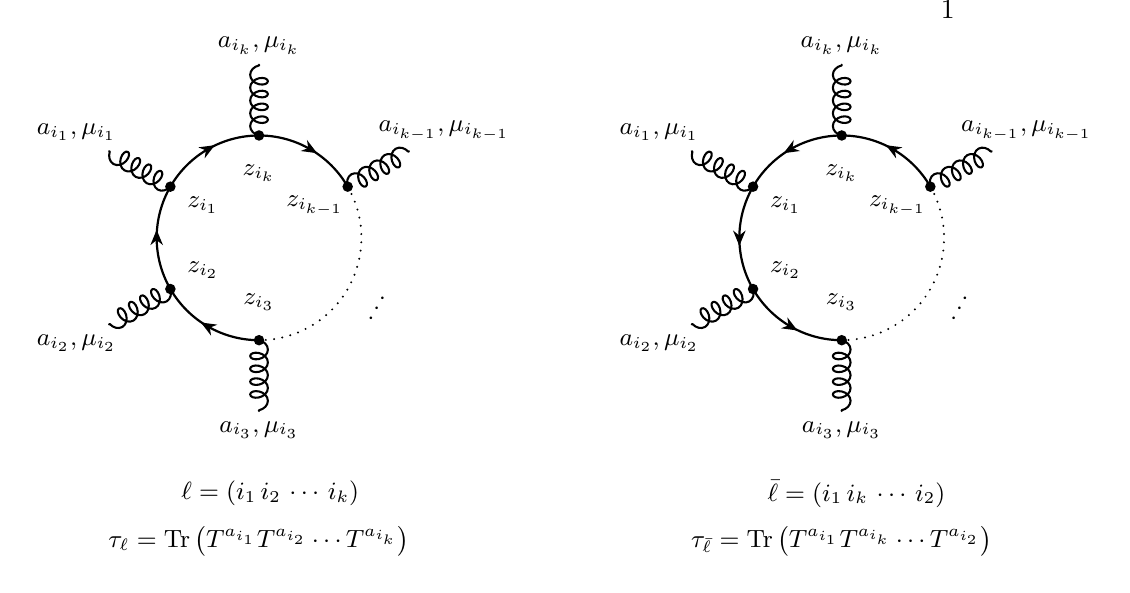
\begin{tikzpicture}[fd]
  \def\fdR{1.3}\def\fdL{0.9}
  % ---------- left panel: orientation \ell, arrows clockwise ----------
  \begin{scope}
    \draw[quark] (210:\fdR) arc[start angle=210,end angle=150,radius=\fdR];
    \draw[quark] (270:\fdR) arc[start angle=270,end angle=210,radius=\fdR];
    \draw[quark] (150:\fdR) arc[start angle=150,end angle=90,radius=\fdR];
    \draw[quark] (90:\fdR) arc[start angle=90,end angle=30,radius=\fdR];
    \draw[line width=0.8pt,dash pattern=on 0pt off 3pt] (30:\fdR) arc[start angle=30,end angle=-90,radius=\fdR];
    \node[rotate=60] at (330:\fdR+0.45) {$\cdots$};
    \foreach \ang/\idx in {150/{i_1},210/{i_2},270/{i_3},30/{i_{k-1}},90/{i_k}}{
      \draw[gluon] (\ang:\fdR) -- (\ang:\fdR+\fdL);
      \node[vertex] at (\ang:\fdR) {};
      \node[inner sep=1pt] at (\ang:\fdR-0.48) {$z_{\idx}$};}
    \node[above] at (90:\fdR+\fdL) {$a_{i_k},\mu_{i_k}$};
    \node[anchor=-30] at (150:\fdR+\fdL) {$a_{i_1},\mu_{i_1}$};
    \node[anchor=30] at (210:\fdR+\fdL) {$a_{i_2},\mu_{i_2}$};
    \node[below] at (270:\fdR+\fdL) {$a_{i_3},\mu_{i_3}$};
    \node[anchor=-150] at (30:\fdR+\fdL) {$a_{i_{k-1}},\mu_{i_{k-1}}$};
    \node at (0,-3.25) {取向 $\ell=(i_1\,i_2\,\cdots\,i_k)$};
    \node at (0,-3.85) {$\tau_\ell=\Tr\big(T^{a_{i_1}}T^{a_{i_2}}\cdots T^{a_{i_k}}\big)$};
  \end{scope}
  % ---------- right panel: orientation \bar\ell, arrows counterclockwise ----------
  \begin{scope}[xshift=7.4cm]
    \draw[quark] (150:\fdR) arc[start angle=150,end angle=210,radius=\fdR];
    \draw[quark] (210:\fdR) arc[start angle=210,end angle=270,radius=\fdR];
    \draw[quark] (90:\fdR) arc[start angle=90,end angle=150,radius=\fdR];
    \draw[quark] (30:\fdR) arc[start angle=30,end angle=90,radius=\fdR];
    \draw[line width=0.8pt,dash pattern=on 0pt off 3pt] (30:\fdR) arc[start angle=30,end angle=-90,radius=\fdR];
    \node[rotate=60] at (330:\fdR+0.45) {$\cdots$};
    \foreach \ang/\idx in {150/{i_1},210/{i_2},270/{i_3},30/{i_{k-1}},90/{i_k}}{
      \draw[gluon] (\ang:\fdR) -- (\ang:\fdR+\fdL);
      \node[vertex] at (\ang:\fdR) {};
      \node[inner sep=1pt] at (\ang:\fdR-0.48) {$z_{\idx}$};}
    \node[above] at (90:\fdR+\fdL) {$a_{i_k},\mu_{i_k}$};
    \node[anchor=-30] at (150:\fdR+\fdL) {$a_{i_1},\mu_{i_1}$};
    \node[anchor=30] at (210:\fdR+\fdL) {$a_{i_2},\mu_{i_2}$};
    \node[below] at (270:\fdR+\fdL) {$a_{i_3},\mu_{i_3}$};
    \node[anchor=-150] at (30:\fdR+\fdL) {$a_{i_{k-1}},\mu_{i_{k-1}}$};
    \node at (0,-3.25) {反向圈 $\bar\ell=(i_1\,i_k\,\cdots\,i_2)$};
    \node at (0,-3.85) {$\tau_{\bar\ell}=\Tr\big(T^{a_{i_1}}T^{a_{i_k}}\cdots T^{a_{i_2}}\big)$};
  \end{scope}
\end{tikzpicture}
\caption{同一个闭合夸克圈的两种取向（\cref{def:loop-factor}）。顶点按逆时针方向依次为 $z_{i_1},z_{i_2},z_{i_3},\dots,z_{i_k}$，
顶点 $z_{i_j}$ 上的胶子带色指标 $a_{i_j}$ 与 Lorentz 指标 $\mu_{i_j}$。
左：取向 $\ell$，$\psi(z_{i_j})$ 与 $\bar\psi(z_{i_{j+1}})$ 缩并，费米子数由 $z_{i_{j+1}}$ 流向 $z_{i_j}$（顺时针）；
右：反向圈 $\bar\ell$（逆时针）。色矩阵逆着费米子箭头读出，故两者的色因子互为反序迹，$\tau_{\bar\ell}=\Tr(T^{a_{i_k}}\cdots T^{a_{i_2}}T^{a_{i_1}})$；
两种取向的圈因子带有同一个因子 $-1$。}
\label{fig:loop-orientations}
\end{figure}

\paragraph{鬼场圈。}
去掉胶子场后，鬼场--胶子顶点是 Grassmann 奇场的双线性型 $(\partial^\nu\bar c^a)\cdot\ii gf^{abc}\cdot c^c$，只是其中的导数作用在 $\bar c$ 上。
\cref{prop:app-wick-cycles}对任意双线性核成立，所以鬼场有与\cref{lem:closed-loops}相同的循环展开（\cref{app:wick-ghost}）：若不含外鬼场，把每个鬼场顶点的 $c$-槽位与 $\bar c$-槽位都等同于该顶点，
则 $\sigma$ 是鬼场顶点的置换；设 $\sigma$ 的一个循环 $\lambda=(s_1\,s_2\,\cdots\,s_k)$（顶点 $w_{s_j}$ 的 $c$ 与顶点 $w_{s_{j+1}}$ 的 $\bar c$ 缩并）经过 $k$ 个鬼场--胶子顶点，顶点 $w_{s_j}$ 上的胶子带指标 $(b_j,\nu_j)$，则该循环贡献
\begin{equation}\label{eq:setup-ghost-loop}
\begin{aligned}
L^{\mathrm{gh}}_\lambda&=-(\ii g)^k\,f^{e_1b_1e_2}f^{e_2b_2e_3}\cdots f^{e_kb_ke_1}\,\prod_{j=1}^{k}\partial^{\nu_{j+1}}_{w_{s_{j+1}}}\Delta_0\bigl(w_{s_j}-w_{s_{j+1}}\bigr)\\
&=-g^k\,\Tr\bigl(F^{b_1}F^{b_2}\cdots F^{b_k}\bigr)\,\prod_{j=1}^{k}\partial^{\nu_{j+1}}_{w_{s_{j+1}}}\Delta_0\bigl(w_{s_j}-w_{s_{j+1}}\bigr)
\end{aligned}
\end{equation}
（下标模 $k$）。第二个等号来自\cref{eq:setup-adjoint}：$f^{ebe'}=-\ii(F^b)_{ee'}$，故 $f^{e_1b_1e_2}\cdots f^{e_kb_ke_1}$ 等于 $(-\ii)^k$ 乘以伴随表示中的迹，而 $(\ii g)^k(-\ii)^k=g^k$；
例如 $k=3$ 时这一乘积等于 $-\frac N2f^{b_1b_2b_3}$，即 $\Tr(F^{b_1}F^{b_2}F^{b_3})=\frac{\ii N}{2}f^{b_1b_2b_3}$（\cref{eq:app-traces-FFF}）。于是每个闭合鬼场圈带一个因子 $-1$，其色因子是由 $f^{abc}$ 构成的网络，
由\cref{lem:contraction}(iii)，它对\emph{每一种取向分别}是 C~偶的。因此鬼场圈不需要把两种取向配对（两种取向的运动学因子也不同，
因为导数总作用在出射鬼场上），Furry 型的相消只发生在夸克圈上（\cref{sec:thmII}）。

%% ======================================================================
%% 第 3 节  Dirac 空间中的电荷共轭
%% ======================================================================
\section{Dirac 空间中的电荷共轭}\label{sec:dirac}

本节为 Furry 定理准备 Dirac 空间中的全部代数工具。闭合夸克圈反向时，圈因子中矩阵乘积的次序被整体倒转（\cref{def:loop-factor}）。转置反序且保迹，但把 $\gamma^\mu$ 变为 $(\gamma^\mu)^{\tp}$；再用电荷共轭矩阵 $C$ 作相似变换把它拉回 $-\gamma^\mu$，就得到 Clifford 共轭 $X\mapsto\Cconj X=CX^{\tp}C^{-1}$。后文只用到它的四条性质：(i) 它是线性反自同构且为对合，$\Cconj{XY}=\Cconj Y\,\Cconj X$，$\Cconj{\Cconj X}=X$；(ii) $\Cconj{\gamma^\mu}=-\gamma^\mu$，从而常见的顶点矩阵满足 $\Cconj\Gamma=\eta_\Gamma\Gamma$，$\eta_\Gamma=\pm1$；(iii) $\TrD\Cconj X=\TrD X$；(iv) $\Cconj{S(p)}=S(-p)$。四维中它们由矩阵 $C$ 实现（\cref{sec:dirac-cmatrix}至\cref{sec:dirac-propagator}）；维数正规化中既没有也不需要这样的矩阵，(i)--(iv) 改由形式 Clifford 代数上的纯代数论证得到（\cref{sec:dirac-dimreg}）。\cref{sec:dirac-loop}把它们组合成 Dirac 圈的反向公式，即单圈 Furry 定理（\cref{thm:furry-single}）在 Dirac 空间中的全部内容；色空间中的对应部分见\cref{sec:color}。记号同\cref{sec:setup}：$g=\mathrm{diag}(+1,-1,-1,-1)$，$\gamma^5=\ii\gamma^0\gamma^1\gamma^2\gamma^3$，$\sigma^{\mu\nu}=\tfrac{\ii}{2}[\gamma^\mu,\gamma^\nu]$，$\sla p=\gamma^\mu p_\mu$。四维中“表示”指满足 Clifford 关系 $\{\gamma^\mu,\gamma^\nu\}=2g^{\mu\nu}\mathbb 1$ 的任意一组 $4\times4$ 复矩阵；Dirac 表示的显式矩阵与若干辅助引理见\cref{app:dirac}。

% ---------------------------------------------------------------------
\subsection{电荷共轭矩阵与 Clifford 共轭}\label{sec:dirac-cmatrix}

\begin{lemma}[电荷共轭矩阵与 Clifford 共轭]\label{lem:C-matrix}
在 Dirac 表示中取 $C=\ii\gamma^2\gamma^0$，则 $C^{\tp}=C^\dagger=C^{-1}=-C$，且
\begin{equation}\label{eq:C-def}
C\,(\gamma^\mu)^{\tp}\,C^{-1}=-\gamma^\mu\qquad(\mu=0,1,2,3).
\end{equation}
（在任意表示中，满足\cref{eq:C-def}的 $C$ 在相差一个非零常数因子的意义下唯一，且总有 $C^{\tp}=-C$。）
对 $4\times4$ 矩阵 $X$ 定义其 Clifford 共轭 $\Cconj X:=C\,X^{\tp}C^{-1}$。则 $X\mapsto\Cconj X$ 是线性反自同构：
$\Cconj{XY}=\Cconj Y\,\Cconj X$，$\Cconj{\Cconj X}=X$，$\Cconj{\gamma^\mu}=-\gamma^\mu$，并且 $\TrD\Cconj X=\TrD X$。
\end{lemma}

\begin{proof}
第一步在 Dirac 表示中直接验证；第二步导出 Clifford 共轭的代数性质，只用到\cref{eq:C-def}；第三、四步证明括号中关于任意表示的论断；第五步证明迹不变。

\emph{第一步：Dirac 表示。}在 Dirac 表示中（\cref{app:dirac-rep}），$\gamma^0,\gamma^2$ 对称而 $\gamma^1,\gamma^3$ 反对称，即
\begin{equation}\label{eq:dirac-transpose}
(\gamma^\mu)^{\tp}=s_\mu\gamma^\mu,\qquad (s_0,s_1,s_2,s_3)=(+1,-1,+1,-1);
\end{equation}
又 $(\gamma^0)^\dagger=\gamma^0$，$(\gamma^2)^\dagger=-\gamma^2$，$(\gamma^0)^2=-(\gamma^2)^2=\mathbb 1$。于是
\[
C^{\tp}=\ii\gamma^0\gamma^2=-C,\qquad C^\dagger=-\ii\gamma^0(-\gamma^2)=-C,\qquad C^2=-\gamma^2\gamma^0\gamma^2\gamma^0=(\gamma^2)^2(\gamma^0)^2=-\mathbb 1,
\]
故 $C^{-1}=-C$，$C^{\tp}=C^\dagger=C^{-1}=-C$。又 $C\gamma^\mu C^{-1}=\gamma^2\gamma^0\gamma^\mu\gamma^2\gamma^0=-s_\mu\gamma^\mu$（对 $\mu=0,2$ 直接相乘；对 $\mu=1,3$ 先把最右边的 $\gamma^0$ 反对易到 $\gamma^\mu$ 左侧，再用 $\gamma^2\gamma^\mu\gamma^2=\gamma^\mu$），与\cref{eq:dirac-transpose}合起来即 $C(\gamma^\mu)^{\tp}C^{-1}=-s_\mu^2\gamma^\mu=-\gamma^\mu$。逐块的验证见\cref{app:dirac-C}。

\emph{第二步：Clifford 共轭的代数性质。}设在某个表示中可逆矩阵 $C$ 满足\cref{eq:C-def}（不假定 $C$ 的对称性），令 $\Cconj X=CX^{\tp}C^{-1}$。(a) 它是 $\mathbb C$ 线性的（不含复共轭）。(b) 由 $(XY)^{\tp}=Y^{\tp}X^{\tp}$ 得 $\Cconj{XY}=(CY^{\tp}C^{-1})(CX^{\tp}C^{-1})=\Cconj Y\,\Cconj X$，且 $\Cconj{\mathbb 1}=\mathbb 1$。(c) $\Cconj{\gamma^\mu}=-\gamma^\mu$ 就是\cref{eq:C-def}。(d) 把 $C$ 换成 $\kappa C$（$\kappa\neq0$）不改变 $\Cconj X$。由 (b)(c)，对单项式 $X=\gamma^{\mu_1}\gamma^{\mu_2}\cdots\gamma^{\mu_n}$ 有
\begin{equation}\label{eq:dirac-monomial}
\Cconj X=(-1)^n\,\gamma^{\mu_n}\cdots\gamma^{\mu_2}\gamma^{\mu_1}.
\end{equation}
(e) 对合性：$X\mapsto\Cconj{\Cconj X}$ 是两个反自同构的复合，因而是自同构，并且在生成元上是恒等的：$\Cconj{\Cconj{\gamma^\mu}}=-\Cconj{\gamma^\mu}=\gamma^\mu$。由于 $\gamma^\mu$ 的乘积张成全部 $4\times4$ 矩阵（\cref{lem:app-dirac-basis}），这个自同构是恒等映射，$\Cconj{\Cconj X}=X$；特别地 $X\mapsto\Cconj X$ 是双射。

\emph{第三步：任意表示中 $C$ 的存在与唯一。}设 $\{\gamma^\mu\}$ 是任一表示。矩阵 $-(\gamma^\mu)^{\tp}$ 满足同样的 Clifford 关系：$\{(\gamma^\mu)^{\tp},(\gamma^\nu)^{\tp}\}=(\gamma^\nu\gamma^\mu+\gamma^\mu\gamma^\nu)^{\tp}=2g^{\mu\nu}\mathbb 1$。由 Pauli 基本定理（\cref{lem:app-dirac-pauli}），存在可逆矩阵 $S$ 使 $-(\gamma^\mu)^{\tp}=S\gamma^\mu S^{-1}$ 对一切 $\mu$ 成立，于是 $C:=S^{-1}$ 满足\cref{eq:C-def}。唯一性：若 $C_1,C_2$ 都满足\cref{eq:C-def}，则 $Y:=C_1^{-1}C_2$ 满足 $Y(\gamma^\mu)^{\tp}Y^{-1}=C_1^{-1}(-\gamma^\mu)C_1=(\gamma^\mu)^{\tp}$，即 $Y$ 与一切 $(\gamma^\mu)^{\tp}$ 及其乘积对易；这些乘积是\cref{lem:app-dirac-basis}中基底的转置，张成全部 $4\times4$ 矩阵，而与一切矩阵对易的矩阵是标量矩阵（Schur 引理），故 $C_2=\kappa C_1$，$\kappa\neq0$。

\emph{第四步：$C^{\tp}=-C$。}对\cref{eq:C-def}取转置得 $(C^{\tp})^{-1}\gamma^\mu C^{\tp}=-(\gamma^\mu)^{\tp}$，即 $C^{\tp}$ 也满足\cref{eq:C-def}。由第三步 $C^{\tp}=\lambda C$；再转置一次得 $C=\lambda^2C$，故 $\lambda=\pm1$。为确定符号，注意对任意满足 $\Cconj\Gamma=\eta_\Gamma\Gamma$ 的 $\Gamma$ 有
\begin{equation}\label{eq:dirac-GammaC}
(\Gamma C)^{\tp}=C^{\tp}\Gamma^{\tp}=\lambda\,\bigl(C\Gamma^{\tp}C^{-1}\bigr)C=\lambda\,\eta_\Gamma\,\Gamma C .
\end{equation}
取 $\Gamma$ 为 16 个基矩阵：$\mathbb 1,\gamma^5,\gamma^\mu\gamma^5$（$\eta=+1$，共 $6$ 个）与 $\gamma^\mu,\sigma^{\mu\nu}$（$\mu<\nu$；$\eta=-1$，共 $10$ 个）。这些 C~宇称的计算即\cref{lem:C-parity}的证明，它只用到第二步的 (b)(c)，与 $C$ 的对称性无关，故这里没有循环论证。由于 16 个基矩阵线性无关（\cref{lem:app-dirac-basis}）且 $C$ 可逆，16 个矩阵 $\Gamma C$ 构成 $4\times4$ 矩阵空间的一组基，且由\cref{eq:dirac-GammaC}每一个都是对称或反对称的。若 $\lambda=+1$，则 $10$ 个线性无关的矩阵 $\gamma^\mu C,\sigma^{\mu\nu}C$ 都反对称，但 $4\times4$ 反对称矩阵只构成 $6$ 维空间，矛盾。故 $\lambda=-1$，$C^{\tp}=-C$；此时 $10$ 个 $\gamma^\mu C,\sigma^{\mu\nu}C$ 对称、$6$ 个 $C,\gamma^5C,\gamma^\mu\gamma^5C$ 反对称，恰与对称（$10$ 维）与反对称（$6$ 维）矩阵空间的维数吻合（\cref{tab:app-dirac-basis}）。

\emph{第五步：迹。}由矩阵迹的循环性与转置不变性，$\TrD\Cconj X=\TrD(X^{\tp}C^{-1}C)=\TrD X^{\tp}=\TrD X$。
\end{proof}

\begin{remark}[Clifford 共轭的内在刻画]\label{rem:dirac-intrinsic}
由\cref{eq:dirac-monomial}，计算 $\Cconj X$ 无须任何矩阵：把 $X$ 写成 $\gamma$ 乘积的线性组合，各乘积反序，再把每个 $\gamma^\mu$ 换成 $-\gamma^\mu$。它是满足 $\gamma^\mu\mapsto-\gamma^\mu$ 的唯一反自同构，即 Clifford 代数中“反序”（reversion）与“阶对合”（grade involution，$\gamma^\mu\mapsto-\gamma^\mu$）的复合，“Clifford 共轭”之名即来源于此；因此它与 $C$ 的归一化及表示的选取无关（\cref{app:dirac-repindep}），并可直接推广到维数正规化（\cref{def:dimreg-trace}）。它是 $\mathbb C$ 线性的，与反线性的 Dirac 共轭 $X\mapsto\gamma^0X^\dagger\gamma^0$ 不同。至于矩阵 $C$ 本身哪些性质依赖于表示（如 $C^2\propto\mathbb 1$ 与公式 $C=\ii\gamma^2\gamma^0$），见\cref{app:dirac-repindep}；本文的证明只用到在任意表示中成立的\cref{eq:C-def}与 $C^{\tp}=-C$，以及（仅在涉及 Dirac 共轭时）$C$ 的酉性，后者在满足 $(\gamma^\mu)^\dagger=\gamma^0\gamma^\mu\gamma^0$ 的表示中总可经归一化实现。
\end{remark}

% ---------------------------------------------------------------------
\subsection{Dirac 矩阵的 C~宇称}\label{sec:dirac-parity}

因为 $X\mapsto\Cconj X$ 是对合，若 $\Gamma\neq0$ 且 $\Cconj\Gamma=\eta\Gamma$，则 $\Gamma=\Cconj{\Cconj\Gamma}=\eta^2\Gamma$，故 $\eta=\pm1$ 是自动的。

\begin{lemma}[Dirac 矩阵的 C~宇称]\label{lem:C-parity}
若 $\Cconj\Gamma=\eta_\Gamma\,\Gamma$，称 $\eta_\Gamma\in\{\pm1\}$ 为 $\Gamma$ 的 C~宇称。
对 $\mathbb 1,\ \gamma^5,\ \ii\gamma^5,\ \gamma^\mu\gamma^5$ 有 $\eta=+1$；对 $\gamma^\mu,\ \sigma^{\mu\nu},\ \sigma^{\mu\nu}\gamma^5$ 有 $\eta=-1$（见\cref{tab:C-parity}）。
\end{lemma}

\begin{proof}
只用到\cref{lem:C-matrix}证明第二步中的两条性质：$X\mapsto\Cconj X$ 是线性反自同构，且 $\Cconj{\gamma^\mu}=-\gamma^\mu$。
(1) $\Cconj{\mathbb 1}=\mathbb 1$，$\Cconj{\gamma^\mu}=-\gamma^\mu$。
(2) 两个 $\gamma$ 之积反序，两个因子各变一次号：$\Cconj{\gamma^\mu\gamma^\nu}=\gamma^\nu\gamma^\mu$，故 $\Cconj{\sigma^{\mu\nu}}=\tfrac{\ii}{2}(\gamma^\nu\gamma^\mu-\gamma^\mu\gamma^\nu)=-\sigma^{\mu\nu}$。
(3) 由\cref{eq:dirac-monomial}，$\Cconj{\gamma^5}=\ii(-1)^4\gamma^3\gamma^2\gamma^1\gamma^0$；把四个两两反对易的因子完全反序需要 $4\cdot3/2=6$ 次相邻对换，故 $\gamma^3\gamma^2\gamma^1\gamma^0=\gamma^0\gamma^1\gamma^2\gamma^3$，$\Cconj{\gamma^5}=\gamma^5$；由线性，$\Cconj{\ii\gamma^5}=\ii\gamma^5$。
(4) $\Cconj{\gamma^\mu\gamma^5}=\Cconj{\gamma^5}\,\Cconj{\gamma^\mu}=-\gamma^5\gamma^\mu=\gamma^\mu\gamma^5$，用到 $\{\gamma^5,\gamma^\mu\}=0$。
(5) $\Cconj{\sigma^{\mu\nu}\gamma^5}=\Cconj{\gamma^5}\,\Cconj{\sigma^{\mu\nu}}=-\gamma^5\sigma^{\mu\nu}=-\sigma^{\mu\nu}\gamma^5$，用到 $[\gamma^5,\sigma^{\mu\nu}]=0$（$\gamma^5$ 与每个 $\gamma$ 反对易，故与两个 $\gamma$ 之积对易）。
\end{proof}

更一般地，对 $r$ 个两两不同的指标，由\cref{eq:dirac-monomial}及完全反序所需的 $r(r-1)/2$ 次相邻对换，
\begin{equation}\label{eq:dirac-grade}
\Cconj{\bigl(\gamma^{\nu_1}\cdots\gamma^{\nu_r}\bigr)}=(-1)^r\gamma^{\nu_r}\cdots\gamma^{\nu_1}=(-1)^{r(r+1)/2}\,\gamma^{\nu_1}\cdots\gamma^{\nu_r},
\end{equation}
即 $r=0,\dots,4$ 时 $\eta=+,-,-,+,+$，与\cref{lem:C-parity}一致（如 $\gamma^0\gamma^5=\ii\gamma^1\gamma^2\gamma^3$ 对应 $r=3$，$\sigma^{01}\gamma^5=-\gamma^2\gamma^3$ 对应 $r=2$）；这一推导对形式 $D$ 维代数中的反对称化乘积同样成立。另有两条推论。其一，$\sla p+m$ 的 Clifford 共轭为 $-\sla p+m$；手征投影 $P_{L,R}=\tfrac12(\mathbb 1\mp\gamma^5)$ 满足 $\eta=+1$，但 $\Cconj{\gamma^\mu P_L}=-\gamma^\mu P_R$：手征（V$-$A）顶点被映为相反手征的顶点，故具有手征规范耦合的理论没有本文的 C~对称性（\cref{rem:color-anomaly}、\cref{rem:np-nonclaims}）。其二，夸克偶素投影 $\Pi_\Gamma:=(\tfrac12\sla P+m)\Gamma(\tfrac12\sla P-m)$ 满足 $\Cconj{\Pi_\Gamma}=\eta_\Gamma\Pi_\Gamma$（证明见\cref{prop:app-quarkonium}(i)），故 ${}^3S_1$（$\Gamma=\sla\varepsilon$）与 ${}^1S_0$（$\Gamma=\gamma^5$）投影的 C~宇称分别为 $-1$ 与 $+1$（\cref{prop:app-quarkonium}）。

\begin{table}[htbp]
\centering
\caption{Dirac 矩阵的 C~宇称 $\eta_\Gamma$（$\Cconj\Gamma=\eta_\Gamma\Gamma$）及相应双线性型的类型。由\cref{lem:bilinear}，$\eta_\Gamma$ 也是味对角的色单态双线性型 $\bar\psi\Gamma\psi$ 的 C~宇称，与通常教科书中的结果一致（参见\cite[第~3.6~节]{PeskinSchroeder1995}）。$F_{\mu\nu}$ 为电磁场强。最后一行：手征耦合没有确定的 C~宇称。}
\label{tab:C-parity}
\small
\begin{tabularx}{\textwidth}{@{}l c l X@{}}
\toprule
$\Gamma$ & $\eta_\Gamma$ & 双线性型 & 典型的顶点或算符 \\
\midrule
$\mathbb 1$ & $+1$ & S（标量） & 质量项 $m\bar\psi\psi$；Higgs--夸克顶点 \\
$\gamma^5$，$\ii\gamma^5$ & $+1$ & P（赝标量） & 赝标量密度 $\bar\psi\,\ii\gamma^5\psi$；${}^1S_0$ 夸克偶素投影 $\Pi_{\gamma^5}$ \\
$\gamma^\mu$ & $-1$ & V（矢量） & 夸克--胶子顶点 $\ii g\gamma^\mu T^a$ 的 Dirac 部分；光子顶点 $-\ii eQ\gamma^\mu$；$Z$ 的矢量耦合；${}^3S_1$ 投影 $\Pi_{\sla\varepsilon}$ \\
$\gamma^\mu\gamma^5$ & $+1$ & A（轴矢量） & 轴矢流 $\bar\psi\gamma^\mu\gamma^5\psi$；$Z$ 的轴矢耦合；VVA 三角图中的 A 顶点 \\
$\sigma^{\mu\nu}$ & $-1$ & T（张量） & 磁矩型算符 $\bar\psi\sigma^{\mu\nu}\psi\,F_{\mu\nu}$ \\
$\sigma^{\mu\nu}\gamma^5$ & $-1$ & T（赝张量） & 电偶极矩型算符 $\bar\psi\,\ii\sigma^{\mu\nu}\gamma^5\psi\,F_{\mu\nu}$ \\
\midrule
$\gamma^\mu P_L$ & 无 & V$-$A & $W$ 玻色子耦合；$\Cconj{\gamma^\mu P_L}=-\gamma^\mu P_R$，不是 Clifford 共轭的本征元 \\
\bottomrule
\end{tabularx}
\end{table}

% ---------------------------------------------------------------------
\subsection{双线性型的电荷共轭}\label{sec:dirac-bilinear}

在路径积分中，$\psi_{\alpha i}(x)$ 与 $\bar\psi_{\alpha i}(x)$（$\alpha$ 为 Dirac 指标，$i$ 为色指标）是相互独立的 Grassmann 生成元，没有先验的关系 $\bar\psi=\psi^\dagger\gamma^0$。电荷共轭定义为生成元的线性代换
\begin{equation}\label{eq:dirac-Cfields}
\psi_{\alpha i}\longmapsto C_{\alpha\beta}\,\bar\psi_{\beta i},\qquad
\bar\psi_{\alpha i}\longmapsto-\psi_{\beta i}\,(C^{-1})_{\beta\alpha},
\end{equation}
即 $\psi\to C\bar\psi^{\tp}$，$\bar\psi\to-\psi^{\tp}C^{-1}$（$C$ 在色空间中作用为单位矩阵），并延拓为 Grassmann 代数上保持分次的代数自同构。代换本身不涉及次序问题，一切符号都来自乘积的重新排序。以下对重复指标求和。

\begin{lemma}[双线性型的电荷共轭]\label{lem:bilinear}
在 Grassmann 场的变换 $\psi\to C\bar\psi^{\tp}$，$\bar\psi\to-\psi^{\tp}C^{-1}$ 下，对 Dirac 矩阵 $\Gamma$ 与色矩阵 $M$ 有
\begin{equation}\label{eq:bilinear}
\bar\psi\,(\Gamma\otimes M)\,\psi\ \longmapsto\ \bar\psi\,\bigl(\Cconj\Gamma\otimes M^{\tp}\bigr)\,\psi .
\end{equation}
特别地，$\bar\psi\Gamma\psi\mapsto\eta_\Gamma\,\bar\psi\Gamma\psi$，$\bar\psi\gamma^\mu T^a\psi\mapsto-\bar\psi\gamma^\mu(T^a)^{\tp}\psi$。
（在算符形式中，须对流取正规乘积，见\cref{sec:nonpert}。）
\end{lemma}

\begin{proof}
我们证明一个稍强、后文也要用到的结论。设 $\chi,\lambda$ 是两个（不必相同的）带 Dirac 与色指标的 Grassmann 旋量场，按\cref{eq:dirac-Cfields}定义 $\chi^{\Cop}=C\bar\chi^{\tp}$、$\bar\chi^{\Cop}=-\chi^{\tp}C^{-1}$，对 $\lambda$ 亦然。对 Dirac~$\otimes$~色空间上的常数矩阵 $X$，记 $X^{\tp}$ 为对两类指标同时转置，$\Cconj X:=(C\otimes\mathbb 1)X^{\tp}(C\otimes\mathbb 1)^{-1}$（对 $X=\Gamma\otimes M$ 即 $\Cconj X=\Cconj\Gamma\otimes M^{\tp}$）。我们证明
\begin{equation}\label{eq:dirac-bilinear-general}
\bar\chi^{\Cop}\,X\,\lambda^{\Cop}=\bar\lambda\,\Cconj X\,\chi .
\end{equation}
用组合指标 $A=(\alpha,i)$、$B=(\beta,j)$ 等，把 $C\otimes\mathbb 1$ 简记为 $C$，逐步记录符号：
\begin{align*}
\bar\chi^{\Cop}_A\,X_{AB}\,\lambda^{\Cop}_B
&\overset{(1)}{=}\bigl[-\chi_{A'}(C^{-1})_{A'A}\bigr]X_{AB}\bigl[C_{BB'}\bar\lambda_{B'}\bigr]
=-\bigl(C^{-1}XC\bigr)_{A'B'}\,\chi_{A'}\bar\lambda_{B'}\\
&\overset{(2)}{=}+\bigl(C^{-1}XC\bigr)_{A'B'}\,\bar\lambda_{B'}\chi_{A'}
=\bar\lambda_{B'}\bigl[(C^{-1}XC)^{\tp}\bigr]_{B'A'}\chi_{A'}
=\bar\lambda\,C^{\tp}X^{\tp}(C^{-1})^{\tp}\chi\\
&\overset{(3)}{=}\bar\lambda\,CX^{\tp}C^{-1}\chi=\bar\lambda\,\Cconj X\,\chi .
\end{align*}
其中 (1) 代入\cref{eq:dirac-Cfields}，$\bar\chi\mapsto-\chi^{\tp}C^{-1}$ 贡献一个因子 $-1$；(2) 交换两个 Grassmann 变量，$\chi_{A'}\bar\lambda_{B'}=-\bar\lambda_{B'}\chi_{A'}$，再贡献一个 $-1$；(3) $C^{\tp}=-C$ 与 $(C^{-1})^{\tp}=(C^{\tp})^{-1}=-C^{-1}$ 贡献两个 $-1$。四个符号之积为 $+1$。取 $\chi=\lambda=\psi$、$X=\Gamma\otimes M$ 即得\cref{eq:bilinear}；$M=\mathbb 1$ 时由 C~宇称的定义得 $\bar\psi\Gamma\psi\mapsto\eta_\Gamma\bar\psi\Gamma\psi$；$\Gamma=\gamma^\mu$、$M=T^a$ 时由 $\Cconj{\gamma^\mu}=-\gamma^\mu$ 得最后一式。
\end{proof}

\begin{remark}[Grassmann 符号、相对负号与整体相位]\label{rem:dirac-phase}
(1) 第 (2) 步的 Grassmann 符号是本质的：若把 $\psi,\bar\psi$ 当作对易的 c 数，同样的代换给出 $-\eta_\Gamma\bar\psi\Gamma\psi$。
(2) 第 (3) 步其实只用到 $C^{\tp}=\pm C$（两个符号总相消）；$C^{\tp}=-C$ 的作用是保证\cref{eq:dirac-Cfields}为对合：$\psi\mapsto C\bar\psi^{\tp}\mapsto C(-\psi^{\tp}C^{-1})^{\tp}=-C(C^{\tp})^{-1}\psi=\psi$，$\bar\psi\mapsto-\psi^{\tp}C^{-1}\mapsto-\bar\psi\,C^{\tp}C^{-1}=\bar\psi$。
(3) 相对负号不是约定。在算符形式中，由 $(\gamma^0)^*=(\gamma^0)^{\tp}$、$C^\dagger=C^{-1}$ 及由\cref{eq:C-def}得到的 $(\gamma^0)^{\tp}C^{-1}=-C^{-1}\gamma^0$，$C\bar\psi^{\tp}=C(\gamma^0)^{\tp}\psi^*$ 的 Dirac 共轭为 $\psi^{\tp}(\gamma^0)^{\tp}C^{-1}\gamma^0=-\psi^{\tp}C^{-1}$（$\gamma^0$ 为 Hermite 矩阵、$C$ 为酉矩阵的任何表示中成立）；若改取 $\bar\psi\mapsto+\psi^{\tp}C^{-1}$，每个双线性型多出因子 $-1$，夸克作用量整体变号，不再是对称性。
(4) 整体相位无关紧要：$\psi\mapsto\zeta C\bar\psi^{\tp}$，$\bar\psi\mapsto-\zeta'\psi^{\tp}C^{-1}$（$\zeta\zeta'=1$；算符形式中 $\zeta'=\zeta^*$）给出同样的\cref{eq:bilinear}。例如在\cite[第~3.6~节]{PeskinSchroeder1995}中，电荷共轭把 $\psi$ 变为 $-\ii\gamma^2\psi^*$，而本文 $C\bar\psi^{\tp}=\ii\gamma^2\psi^*$（Dirac 表示），相当于 $\zeta=-1$。
\end{remark}

\begin{remark}[推论：色八重态流、导数项、味矩阵]\label{rem:dirac-octet}
(1) 由\cref{def:phi-R}，$-(T^a)^{\tp}=\varphi(T^a)=R^{ab}T^b$，故 $J^{a\mu}:=\bar\psi\gamma^\mu T^a\psi\mapsto R^{ab}J^{b\mu}$，与胶子场 $A^a_\mu\mapsto R^{ab}A^b_\mu$（\cref{eq:C-fields}）的变换方式相同：Dirac 空间的 $\eta_{\gamma^\mu}=-1$ 被色自同构 $\varphi(X)=-X^{\tp}$ 的负号吸收。这正是胶子场的变换是 $A_\mu\mapsto-A_\mu^{\tp}$ 而不是 $A_\mu\mapsto-A_\mu$ 的原因；由 $R$ 的正交性，$gA^a_\mu J^{a\mu}$ 不变（\cref{prop:L-invariance}）。
(2) \cref{eq:dirac-bilinear-general}不要求 $\chi=\lambda$，故也适用于导数项（取 $\chi=\psi$、$\lambda=\partial_\mu\psi$，见\cref{prop:L-invariance}证明的第二步，即\cref{eq:np-kinetic}）。又因 $\Cconj{\sigma^{\mu\nu}}=-\sigma^{\mu\nu}$，$C\bigl(\exp(\tfrac{\ii}{4}\omega_{\mu\nu}\sigma^{\mu\nu})\bigr)^{\tp}C^{-1}=\exp(-\tfrac{\ii}{4}\omega_{\mu\nu}\sigma^{\mu\nu})$，故 $C\bar\psi^{\tp}$ 仍按 Dirac 旋量作 Lorentz 变换。
(3) 若场还带味指标，把它并入组合指标，证明逐字成立：对味矩阵 $\Lambda$（记号同\cref{rem:thmI-flavour}），$\bar\psi\Gamma\Lambda\psi\mapsto\eta_\Gamma\bar\psi\Gamma\Lambda^{\tp}\psi$。味对角（或味对称）的色单态流是 C~本征算符；味改变的流被映为“味转置”的流，$\bar\psi_f\Gamma\psi_{f'}\mapsto\eta_\Gamma\bar\psi_{f'}\Gamma\psi_f$（如 $\bar u\Gamma d\leftrightarrow\bar d\Gamma u$），C~此时只联系两个不同的过程，不给出单个过程的选择定则（参见\cref{rem:thmI-flavour}）。
\end{remark}

\begin{remark}[算符形式与正规乘积]\label{rem:dirac-operator}
在算符形式中，等时反对易关系 $\{\psi(t,\bm x),\bar\psi(t,\bm y)\}=\gamma^0\,\delta^3(\bm x-\bm y)$（色指标上为 $\delta_{ij}$）使第 (2) 步的交换多出一个 c 数。对同一点的双线性型直接计算得
\begin{equation}\label{eq:dirac-cnumber}
\Cop\,\bar\psi(\Gamma\otimes M)\psi\,\Cop^{-1}=\bar\psi\bigl(\Cconj\Gamma\otimes M^{\tp}\bigr)\psi+\TrD(\Gamma\gamma^0)\,\Tr M\;\delta^3(\bm 0),
\end{equation}
其中用到 $\sum_{\alpha\beta}(C^{-1}\Gamma C)_{\alpha\beta}(\gamma^0)_{\alpha\beta}=\TrD[\Gamma\,C(\gamma^0)^{\tp}C^{-1}]=-\TrD(\Gamma\gamma^0)$。额外项只在 $\TrD(\Gamma\gamma^0)\neq0$（在 Clifford 基中即 $\Gamma$ 含 $\gamma^0$ 分量）且 $\Tr M\neq0$ 时（如电荷密度 $\psi^\dagger\psi$）不为零；若 $\Cop$ 为酉算符且 $\Cop|0\rangle=|0\rangle$，取真空期望值可知（$M=\mathbb 1$）它等价于 $\Cop O\Cop^{-1}=\eta_\Gamma O+(1-\eta_\Gamma)\langle0|O|0\rangle$，$O=\bar\psi\Gamma\psi$。对正规乘积，$:\!\psi_A\bar\psi_B\!:\;=-:\!\bar\psi_B\psi_A\!:$ 严格成立，故\cref{eq:bilinear}对正规乘积的流严格成立（详见\cref{sec:nonpert}与\cref{rem:np-operator}）；路径积分中不出现此类项。
\end{remark}

% ---------------------------------------------------------------------
\subsection{传播子的电荷共轭}\label{sec:dirac-propagator}

\begin{lemma}[传播子的电荷共轭]\label{lem:propagator}
对 $S(p)=\ii(\sla p+m)/(p^2-m^2+\ii0)$ 及 $\SF(x)=\int\frac{\dd^4p}{(2\pi)^4}\,\ee^{-\ii p\cdot x}S(p)$，有
\begin{equation}\label{eq:C-prop}
\Cconj{S(p)}=S(-p),\qquad \Cconj{\SF(x)}=\SF(-x).
\end{equation}
\end{lemma}

\begin{proof}
\emph{动量空间。}Clifford 共轭是线性的，不影响标量因子 $\ii/(p^2-m^2+\ii0)$，而 $\Cconj{\sla p+m}=p_\mu\Cconj{\gamma^\mu}+m=-\sla p+m$，故
\[
\Cconj{S(p)}=\frac{\ii(-\sla p+m)}{p^2-m^2+\ii0}=\frac{\ii\bigl(\sla{(-p)}+m\bigr)}{(-p)^2-m^2+\ii0}=S(-p),
\]
因为分母（连同 Feynman 规定 $+\ii0$）是 $p$ 的偶函数；作为有理函数的恒等式，它对极点以外的一切复动量成立。$S(p)$ 在色空间中正比于对称的 $\delta_{ij}$，故在 Dirac~$\otimes$~色空间中同样成立。

\emph{坐标空间。}$\SF(x)=(\ii\sla\partial+m)\Delta_F(x)$，其中 $\Delta_F(x)=\int\frac{\dd^4p}{(2\pi)^4}\,\ii\,\ee^{-\ii p\cdot x}/(p^2-m^2+\ii0)$（因 $\ii\sla\partial\,\ee^{-\ii p\cdot x}=\sla p\,\ee^{-\ii p\cdot x}$）；积分变量代换 $p\to-p$ 表明 $\Delta_F(-x)=\Delta_F(x)$。微分算子作用于标量函数，与矩阵运算可交换，故 $\Cconj{\SF(x)}=(\ii\,\Cconj{\gamma^\mu}\partial_\mu+m)\Delta_F(x)=(-\ii\sla\partial+m)\Delta_F(x)$；另一方面由链式法则，
\[
\SF(-x)=\bigl[(\ii\gamma^\mu\partial/\partial y^\mu+m)\Delta_F(y)\bigr]_{y=-x}=(-\ii\sla\partial+m)\Delta_F(-x)=(-\ii\sla\partial+m)\Delta_F(x).
\]
等价地，Clifford 共轭对 $16$ 个矩阵元作用为常系数线性变换，与（缓增分布意义下的）Fourier 积分可交换，于是 $\Cconj{\SF(x)}=\int\frac{\dd^4p}{(2\pi)^4}\ee^{-\ii p\cdot x}S(-p)=\SF(-x)$（作代换 $p\to-p$）。
\end{proof}

\begin{remark}[正规化的传播子与两点插入]\label{rem:dirac-regprop}
\cref{lem:propagator}的直观意义是：经电荷共轭的传播子就是动量反号的传播子，“正向运动的反夸克”等价于“逆着箭头走的夸克线”。证明只用到 $S(p)$ 的如下结构：它是 $\mathbb 1$ 与一个 $\gamma$ 的组合，标量部分为 $p$ 的偶函数、矢量部分为奇函数。因此任何 $F(p)=a(p)\mathbb 1+b_\mu(p)\gamma^\mu$（$a$ 偶、$b_\mu$ 奇）都满足 $\Cconj{F(p)}=F(-p)$，这包括 Pauli--Villars 组合\cite{PauliVillars1949} $\sum_ic_iS(p;M_i)$、维数正规化中的 $D$ 维传播子（此时 $\Cconj X$ 是\cref{def:dimreg-trace}中的形式运算，计算相同）、Wilson 格点费米子的传播子（Euclid 形式，\cref{eq:reg-wilson}），以及形如 $\ii(\delta_2\sla p-\delta_m)$ 的两点抵消项顶点。坐标空间中相应的充分条件是 $S_{\mathrm{reg}}(x)=A(x)\mathbb 1+B_\nu(x)\gamma^\nu$（$A$ 为偶函数、$B_\nu$ 为奇函数），例如 $(\ii\sla\partial+m)\Delta_{\mathrm{reg}}$（$\Delta_{\mathrm{reg}}$ 为偶函数）与 Pauli--Villars 的 $\sum_ic_i(\ii\sla\partial+M_i)\Delta_F(x;M_i)$（\cref{sec:reg-pv}）。性质 $\Cconj{S_{\mathrm{reg}}(p)}=S_{\mathrm{reg}}(-p)$ 及其坐标空间形式 $\Cconj{S_{\mathrm{reg}}(x)}=S_{\mathrm{reg}}(-x)$ 正是\cref{def:reg-hypotheses}中假设 (R1) 关于传播子的条件；上述形式只是它的充分条件。
\end{remark}

% ---------------------------------------------------------------------
\subsection{维数正规化中的 Dirac 代数}\label{sec:dirac-dimreg}

在维数正规化中 $\gamma^\mu$ 带 $D$ 维指标，非整数 $D$ 没有有限维矩阵实现；对偶数整数 $D$，满足 $C(\gamma^\mu)^{\tp}C^{-1}=-\gamma^\mu$ 的矩阵虽然存在，其对称性却依赖于 $D$：$D=4$ 时反对称，$D=6$ 时对称。\cref{lem:C-matrix}第四步的计数论证对任意偶数 $D$ 照样进行，只是结论随 $D$ 而变：$D=6$ 时，由\cref{eq:dirac-grade}，$2^6$ 个反对称化乘积中 C~宇称为 $+1$ 的（$r=0,3,4$）共 $1+20+15=36$ 个、为 $-1$ 的共 $28$ 个，与 $8\times8$ 对称、反对称矩阵空间的维数 $36$、$28$ 相容的只有 $C^{\tp}=+C$（这也已用显式的 $8\times8$ 矩阵核验）。后文需要的不是矩阵 $C$，而是 Clifford 共轭本身（\cref{rem:dirac-intrinsic}）及迹在其下的不变性；下面把它们建立在纯代数的基础上。

\begin{definition}[维数正规化中的 Dirac 代数]\label{def:dimreg-trace}
在 $D=4-2\epsilon$ 维的维数正规化中，$\gamma^\mu$ 是满足 $\{\gamma^\mu,\gamma^\nu\}=2g^{\mu\nu}\mathbb 1$、$g^{\mu}{}_{\mu}=D$ 的形式生成元，
$\TrD$ 是其乘积的线性组合上的泛函，满足：
(T1) 线性；(T2) 循环性 $\TrD(XY)=\TrD(YX)$；(T3) $\TrD\mathbb 1=4$；(T4) 奇数个 $\gamma$ 矩阵之积的迹为零。
并定义 $X\mapsto\Cconj X$ 为满足 $\Cconj{\gamma^\mu}=-\gamma^\mu$ 的线性反自同构。
\end{definition}

“形式生成元”的精确含义如下。设 $\mathcal T$ 为由符号 $\gamma^\mu$（$\mu$ 取遍形式的 $D$ 维指标集）生成的自由结合代数，其单项式 $\gamma^{\mu_1}\cdots\gamma^{\mu_n}$（$n\ge0$）构成 $\mathcal T$ 的基；$\mathcal I\subset\mathcal T$ 是由 $r^{\mu\nu}:=\gamma^\mu\gamma^\nu+\gamma^\nu\gamma^\mu-2g^{\mu\nu}\mathbb 1$ 生成的双边理想；形式 Dirac 代数定义为商代数 $\mathcal A_D:=\mathcal T/\mathcal I$。$\mathcal A_D$ 的元素是单项式的有限线性组合（系数可依赖于动量、质量等），$\TrD$ 的值是度规分量 $g^{\mu\nu}$ 的多项式，指标缩并时 $g^\mu{}_\mu=D$ 给出对 $D$ 的多项式依赖。以下论证都是纯代数的，不涉及任何矩阵或 $D$ 的具体数值；$D=4$ 且一切指标取四维值时，它们给出通常的四维迹。

\begin{lemma}[迹的反序不变性]\label{lem:trace-reversal}
无论在四维还是在\cref{def:dimreg-trace}的形式 $D$ 维 Dirac 代数中，都有 $\TrD\Cconj X=\TrD X$；等价地，对任意 $n$ 与任意指标，
\begin{equation}\label{eq:trace-reversal}
\TrD\bigl(\gamma^{\mu_1}\gamma^{\mu_2}\cdots\gamma^{\mu_n}\bigr)=\TrD\bigl(\gamma^{\mu_n}\cdots\gamma^{\mu_2}\gamma^{\mu_1}\bigr).
\end{equation}
在 $D$ 维情形，公理 (T1)--(T4) 与 Clifford 关系唯一地确定 $\TrD$，而 $X\mapsto\TrD\Cconj X$ 满足同样的公理，故二者相等。
\end{lemma}

\begin{proof}
\emph{两种表述的等价性。}对单项式 $X=\gamma^{\mu_1}\cdots\gamma^{\mu_n}$，\cref{eq:dirac-monomial}给出 $\Cconj X=(-1)^n\gamma^{\mu_n}\cdots\gamma^{\mu_1}$；其推导只用到反自同构性质与 $\Cconj{\gamma^\mu}=-\gamma^\mu$，在 $\mathcal A_D$ 中同样成立。由线性，“$\TrD\Cconj X=\TrD X$ 对一切 $X$ 成立”等价于“$\TrD(\gamma^{\mu_1}\cdots\gamma^{\mu_n})=(-1)^n\TrD(\gamma^{\mu_n}\cdots\gamma^{\mu_1})$ 对一切 $n$ 与指标成立”；由于奇数个 $\gamma$ 之积的迹为零（$D$ 维中即 (T4)，四维中见下），后者又等价于\cref{eq:trace-reversal}。

\emph{证法一：四维。}$\TrD\Cconj X=\TrD X$ 已在\cref{lem:C-matrix}中证明。奇数个 $\gamma$ 之积的迹为零：由 $(\gamma^5)^2=\mathbb 1$、迹的循环性与 $\{\gamma^5,\gamma^\mu\}=0$，$\TrD(\gamma^{\mu_1}\cdots\gamma^{\mu_n})=\TrD(\gamma^5\gamma^{\mu_1}\cdots\gamma^{\mu_n}\gamma^5)=(-1)^n\TrD(\gamma^{\mu_1}\cdots\gamma^{\mu_n})$。由上面的等价性即得\cref{eq:trace-reversal}。

\emph{证法二：$D$ 维。}(a) 唯一性。设 $T$ 是 $\mathcal A_D$ 上任一满足 (T1)--(T4) 的线性泛函。对 $n\ge2$，反复用 $\gamma^{\mu_1}\gamma^{\mu_j}=2g^{\mu_1\mu_j}\mathbb 1-\gamma^{\mu_j}\gamma^{\mu_1}$ 把 $\gamma^{\mu_1}$ 逐个移过右侧的因子，得
\begin{equation}\label{eq:dirac-anticomm}
\gamma^{\mu_1}\gamma^{\mu_2}\cdots\gamma^{\mu_n}
=\sum_{j=2}^{n}(-1)^{j}\,2g^{\mu_1\mu_j}\,\gamma^{\mu_2}\cdots\widehat{\gamma^{\mu_j}}\cdots\gamma^{\mu_n}
+(-1)^{n-1}\,\gamma^{\mu_2}\cdots\gamma^{\mu_n}\gamma^{\mu_1},
\end{equation}
其中 $\widehat{\gamma^{\mu_j}}$ 表示略去该因子；第 $j$ 项来自 $\gamma^{\mu_1}$ 越过 $\gamma^{\mu_2},\dots,\gamma^{\mu_{j-1}}$（符号 $(-1)^{j-2}$）之后与 $\gamma^{\mu_j}$ 的反对易子。对\cref{eq:dirac-anticomm}作用 $T$，由 (T2) 末项等于 $(-1)^{n-1}T(\gamma^{\mu_1}\cdots\gamma^{\mu_n})$。$n$ 为偶数时 $(-1)^{n-1}=-1$，移项后除以 $2$ 得
\begin{equation}\label{eq:dirac-recursion}
T(\gamma^{\mu_1}\gamma^{\mu_2}\cdots\gamma^{\mu_n})=\sum_{j=2}^{n}(-1)^{j}\,g^{\mu_1\mu_j}\,T\bigl(\gamma^{\mu_2}\cdots\widehat{\gamma^{\mu_j}}\cdots\gamma^{\mu_n}\bigr)\qquad(n\ \text{为偶数}).
\end{equation}
由 (T3) 的初值 $T(\mathbb 1)=4$ 对偶数 $n$ 归纳，$T$ 在一切偶数长度的单项式上被唯一确定；由 (T4) 它在奇数长度的单项式上为零；由 (T1) 它在 $\mathcal A_D$ 上被唯一确定。例如 $T(\gamma^\mu\gamma^\nu)=4g^{\mu\nu}$，$T(\gamma^\mu\gamma^\nu\gamma^\rho\gamma^\sigma)=4(g^{\mu\nu}g^{\rho\sigma}-g^{\mu\rho}g^{\nu\sigma}+g^{\mu\sigma}g^{\nu\rho})$。注意 $n$ 为奇数时 $(-1)^{n-1}=+1$，\cref{eq:dirac-anticomm}两边的 $T(\gamma^{\mu_1}\cdots\gamma^{\mu_n})$ 相消，递推不能确定奇数长度的迹，故这里直接用 (T4)。（剩下的关系 $\sum_{j=2}^{n}(-1)^{j}g^{\mu_1\mu_j}\,T(\gamma^{\mu_2}\cdots\widehat{\gamma^{\mu_j}}\cdots\gamma^{\mu_n})=0$ 仍约束较短的奇数长度迹：用 $g_{\mu_1\mu_2}$ 缩并，再用 Clifford 关系把各项中的 $\gamma^{\mu_j}$ 移回原位，得 $(D-n+2)\,T(\gamma^{\mu_3}\cdots\gamma^{\mu_n})$ 等于长度为 $n-4$ 的迹的线性组合。对 $n$ 归纳可知，只要 $D$ 不是奇数整数（$D=4$ 与形式的 $D$ 都是如此），(T4) 其实可由 (T1)、(T2) 与 Clifford 关系推出；在奇数整数维中则不然。）

(b) Clifford 共轭的存在性与良定义性。$\mathcal T$ 是自由代数，故存在唯一的线性反同态 $t:\mathcal T\to\mathcal T$ 使 $t(\gamma^\mu)=-\gamma^\mu$、$t(\mathbb 1)=\mathbb 1$，即 $t(\gamma^{\mu_1}\cdots\gamma^{\mu_n})=(-1)^n\gamma^{\mu_n}\cdots\gamma^{\mu_1}$，且 $t^2=\mathrm{id}$。由 $g^{\mu\nu}=g^{\nu\mu}$，
\begin{gather*}
t(r^{\mu\nu})=(-\gamma^\nu)(-\gamma^\mu)+(-\gamma^\mu)(-\gamma^\nu)-2g^{\mu\nu}\mathbb 1=r^{\mu\nu},\\
t\Bigl(\sum_kx_k\,r^{\mu_k\nu_k}\,y_k\Bigr)=\sum_kt(y_k)\,r^{\mu_k\nu_k}\,t(x_k)\in\mathcal I .
\end{gather*}
故 $t(\mathcal I)\subset\mathcal I$，$t$ 诱导出 $\mathcal A_D$ 上满足 $\Cconj{\gamma^\mu}=-\gamma^\mu$、$\Cconj{\Cconj X}=X$ 的线性反自同构；反自同构由其在生成元上的值唯一确定，故它就是\cref{def:dimreg-trace}中的映射。

(c) 令 $T'(X):=\TrD\Cconj X$。(T1) 显然；(T2)：$T'(XY)=\TrD(\Cconj Y\,\Cconj X)=\TrD(\Cconj X\,\Cconj Y)=T'(YX)$；(T3)：$T'(\mathbb 1)=4$；(T4)：奇数长度单项式的 Clifford 共轭是另一个奇数长度单项式的 $\pm1$ 倍，其迹为零。由 (a)，$T'=\TrD$，即 $\TrD\Cconj X=\TrD X$；再由等价性即得\cref{eq:trace-reversal}。
\end{proof}

\begin{remark}[存在性与配对公式]\label{rem:dirac-pairing}
\cref{def:dimreg-trace}预设了满足 (T1)--(T4) 的泛函存在，这可以显式验证：对偶数 $n$ 令
\begin{equation}\label{eq:dirac-pairing}
\TrD(\gamma^{\mu_1}\cdots\gamma^{\mu_n})=4\sum_{\pi\in\mathcal M_n}(-1)^{\mathrm{cr}(\pi)}\prod_{\{a<b\}\in\pi}g^{\mu_a\mu_b},
\end{equation}
对奇数 $n$ 令其为零；其中 $\mathcal M_n$ 是 $\{1,\dots,n\}$ 的完美配对的集合，把 $1,\dots,n$ 依次放在圆周上、每对连一条弦，$\mathrm{cr}(\pi)$ 为相交的弦对数（两弦相交当且仅当端点在圆周上交错）。(i) 与弦 $\{1,j\}$ 相交的弦就是只有一个端点落在 $\{2,\dots,j-1\}$ 中的弦，而该集合的其余点两两被内部的弦占据，故相交弦数与 $j-2$ 同奇偶，\cref{eq:dirac-pairing}满足递推\cref{eq:dirac-recursion}。(ii) 交换相邻位置 $a,a+1$ 的因子时，含弦 $\{a,a+1\}$ 的配对合计贡献 $2g^{\mu_a\mu_{a+1}}$ 乘以其余因子的迹，其余配对一一对应而交叉数的奇偶性恰好翻转、贡献相消，故它与 Clifford 关系相容；交错关系在圆周旋转下不变，故 (T2) 成立。于是满足公理的泛函存在。(iii) 圆周的反射 $a\mapsto n+1-a$ 也保持交错关系，这给出\cref{eq:trace-reversal}的第三个、纯组合的证明。（这些性质也已用计算机代数对 $n\le12$ 逐项核对。）
\end{remark}

\begin{remark}[$\gamma^5$]\label{rem:dirac-gamma5}
当 $D\neq4$ 时，$\gamma^5$ 与一切 $\gamma^\mu$ 反对易、迹的循环性 (T2) 与 $\TrD(\gamma^5\gamma^\mu\gamma^\nu\gamma^\rho\gamma^\sigma)\neq0$ 三者不能同时成立。事实上，对两两不同的 $\mu,\nu,\rho,\sigma$，Clifford 关系给出 $\gamma_\alpha\gamma^\mu\gamma^\nu\gamma^\rho\gamma^\sigma\gamma^\alpha={(D-8)}\,\gamma^\mu\gamma^\nu\gamma^\rho\gamma^\sigma$，于是由 (T2) 与 $\gamma^5$ 的反对易性，
\[
D\,\TrD(\gamma^5\gamma^\mu\gamma^\nu\gamma^\rho\gamma^\sigma)=\TrD(\gamma_\alpha\gamma^5\gamma^\mu\gamma^\nu\gamma^\rho\gamma^\sigma\gamma^\alpha)=-(D-8)\,\TrD(\gamma^5\gamma^\mu\gamma^\nu\gamma^\rho\gamma^\sigma),
\]
即 $(D-4)\TrD(\gamma^5\gamma^\mu\gamma^\nu\gamma^\rho\gamma^\sigma)=0$（参见\cite{BreitenlohnerMaison1977}）。在 \mbox{'t}~Hooft--Veltman/Breitenlohner--Maison 方案\cite{BreitenlohnerMaison1977,tHooftVeltman1972}中，$\gamma^5:=\ii\gamma^0\gamma^1\gamma^2\gamma^3$ 是 $\mathcal A_D$ 中四个取四维指标的 $\gamma$ 之积，故\cref{lem:trace-reversal}对含 $\gamma^5$ 的迹照样成立，且同\cref{lem:C-parity}有 $\Cconj{\gamma^5}=\gamma^5$。但它与 $\gamma^\mu$ 的 $(D-4)$ 维“消逝”（evanescent）分量 $\hat\gamma^\mu$（\cref{sec:reg-gamma5}）对易，因而未对称化的轴矢顶点 $\gamma^\mu\gamma^5$ 不是 Clifford 共轭的本征元（\cref{eq:reg-bmhv}）；对称化的轴矢顶点（\cref{eq:reg-axial}）与 Larin 处方\cite{Larin1993}中的轴矢顶点（三个 $\gamma$ 的反对称化乘积，由\cref{eq:dirac-grade}）则严格满足 $\eta=+1$。因此在维数正规化中，\cref{prop:loop-reversal}对 $\Gamma_j\in\{\mathbb 1,\gamma^\mu,\sigma^{\mu\nu}\}$ 无条件成立，对 $\gamma^5$、$\ii\gamma^5$ 与对称化的轴矢顶点也成立，但不能直接用于未对称化的 $\gamma^\mu\gamma^5$。详见\cref{sec:reg-gamma5}；VVA 三角图见\cref{sec:applications-other}。
\end{remark}

% ---------------------------------------------------------------------
\subsection{Dirac 圈的反向}\label{sec:dirac-loop}

\begin{proposition}[Dirac 圈的反向]\label{prop:loop-reversal}
设 $\Gamma_1,\dots,\Gamma_k$ 的 C~宇称为 $\eta_1,\dots,\eta_k$，$q_1,\dots,q_k$ 为任意动量。则
\begin{equation}\label{eq:loop-reversal-mom}
\begin{aligned}
&\TrD\bigl[\Gamma_1S(q_1)\Gamma_2S(q_2)\cdots\Gamma_kS(q_k)\bigr]\\
&\qquad=\Bigl(\prod_{j=1}^{k}\eta_j\Bigr)\TrD\bigl[\Gamma_1S(-q_k)\Gamma_kS(-q_{k-1})\Gamma_{k-1}\cdots\Gamma_2S(-q_1)\bigr].
\end{aligned}
\end{equation}
在坐标空间中，对\cref{def:loop-factor}的 Dirac 因子有
\begin{equation}\label{eq:loop-reversal}
K_{\bar\ell}=\Bigl(\prod_{j=1}^{k}\eta_{i_j}\Bigr)K_\ell;\qquad\text{特别地，对只含夸克--胶子顶点的圈，}\ K_{\bar\ell}=(-1)^kK_\ell .
\end{equation}
上述等式在四维、对 Pauli--Villars 正规化的传播子以及在维数正规化中（$\Gamma_j\in\{\mathbb 1,\gamma^\mu,\sigma^{\mu\nu}\}$）逐点成立。
\end{proposition}

\begin{proof}
\emph{第一步：动量空间。}令 $M:=\Gamma_1S(q_1)\Gamma_2S(q_2)\cdots\Gamma_kS(q_k)$。由\cref{lem:C-matrix}（四维）或\cref{lem:trace-reversal}（$D$ 维），$\TrD M=\TrD\Cconj M$。由反自同构性质、$\Cconj{\Gamma_j}=\eta_j\Gamma_j$（\cref{lem:C-parity}）与 $\Cconj{S(q)}=S(-q)$（\cref{lem:propagator}），
\[
\Cconj M=\Cconj{S(q_k)}\,\Cconj{\Gamma_k}\cdots\Cconj{S(q_1)}\,\Cconj{\Gamma_1}
=\Bigl(\prod_{j=1}^k\eta_j\Bigr)S(-q_k)\Gamma_kS(-q_{k-1})\Gamma_{k-1}\cdots S(-q_1)\Gamma_1 .
\]
由循环性把末尾的 $\Gamma_1$ 移到最前，即得\cref{eq:loop-reversal-mom}。这里没有用到 $q_j$ 之间的任何关系（动量守恒、在壳条件或圈积分），等式对每一组固定的动量成立。

\emph{第二步：坐标空间。}记 $\ell=(i_1\,i_2\,\cdots\,i_k)$，则 $\bar\ell=(i_1\,i_k\,\cdots\,i_2)$，按\cref{def:loop-factor}，$K_{\bar\ell}=\TrD P$，
\[
P:=\Gamma_{i_1}\SF(z_{i_1}-z_{i_k})\,\Gamma_{i_k}\SF(z_{i_k}-z_{i_{k-1}})\cdots\Gamma_{i_2}\SF(z_{i_2}-z_{i_1}).
\]
各因子反序，并用 $\Cconj{\Gamma_{i_j}}=\eta_{i_j}\Gamma_{i_j}$ 与 $\Cconj{\SF(z-z')}=\SF(z'-z)$，
\[
\Cconj P=\SF(z_{i_1}-z_{i_2})\,\eta_{i_2}\Gamma_{i_2}\,\SF(z_{i_2}-z_{i_3})\cdots\eta_{i_k}\Gamma_{i_k}\,\SF(z_{i_k}-z_{i_1})\,\eta_{i_1}\Gamma_{i_1}.
\]
由 $\TrD P=\TrD\Cconj P$ 与循环性（把末尾的 $\Gamma_{i_1}$ 移到最前）得 $K_{\bar\ell}=\bigl(\prod_j\eta_{i_j}\bigr)K_\ell$。坐标空间中的乘积在顶点重合处需要正规化；论证对任何满足 $\Cconj{S_{\mathrm{reg}}(x)}=S_{\mathrm{reg}}(-x)$ 的正规化传播子逐字成立（\cref{rem:dirac-regprop}）。

\emph{第三步。}对夸克--胶子顶点 $\Gamma_j=\gamma^{\mu_j}$，$\eta_j=-1$，故 $\prod_j\eta_j=(-1)^k$。适用范围见下文。
\end{proof}

\paragraph{镜像动量配置。}在 $K_\ell$ 中代入 $\SF(z_{i_j}-z_{i_{j+1}})=\int\frac{\dd^4q_j}{(2\pi)^4}\ee^{-\ii q_j\cdot(z_{i_j}-z_{i_{j+1}})}S(q_j)$，$q_j$ 是第 $j$ 条内线上沿费米子箭头（由 $z_{i_{j+1}}$ 指向 $z_{i_j}$）的动量。在 $K_{\bar\ell}$ 中连接同一对顶点的是 $\SF(z_{i_{j+1}}-z_{i_j})$；把积分变量记为 $-q_j$，它成为
\[
\SF(z_{i_{j+1}}-z_{i_j})=\int\!\frac{\dd^4q_j}{(2\pi)^4}\,\ee^{-\ii q_j\cdot(z_{i_j}-z_{i_{j+1}})}\,S(-q_j).
\]
于是两种取向带有完全相同的指数因子，对顶点坐标积分后给出完全相同的动量守恒 $\delta$ 函数：同一条几何内线在两种取向中携带同一个物理动量（在图中沿该线的同一方向流动，即由 $z_{i_{j+1}}$ 流向 $z_{i_j}$），但沿反向后的费米子箭头度量时它是 $-q_j$（\cref{fig:dirac-mirror}）。我们称之为镜像动量配置。在这一配置下，$K_\ell$ 与 $K_{\bar\ell}$ 在动量空间中的被积函数分别是\cref{eq:loop-reversal-mom}左端的迹与右端的迹（右端的迹不含因子 $\prod_j\eta_j$），故反向公式在圈动量积分之前逐点成立。对 $\ell=(1\,2\,\cdots\,k)$、在第 $j$ 个顶点流入的外动量 $p_j$（$\sum_jp_j=0$）与圈动量 $l$，标准的多边形配置为
\begin{equation}\label{eq:dirac-polygon}
q_k=l,\qquad q_{j-1}=q_j+p_j\quad(j=k,\dots,2),\qquad\text{即}\quad q_j=l+\sum_{i=j+1}^{k}p_i ,
\end{equation}
它在每个顶点处满足动量守恒，而 $\bar\ell$ 中同一条线沿其箭头的动量为 $-q_j$。对 $k=3$，$(q_1,q_2,q_3)=(l-p_1,\,l+p_3,\,l)$，\cref{eq:loop-reversal-mom}正是\cref{prop:triangle}中的被积函数恒等式（\cref{eq:triangle-integrand}；那里圈动量记为 $k$，见\cref{fig:triangles}）。对 $\bar\ell$ 采用其他配置时，二者相差圈动量的仿射替换 $l\to\pm l+a$：若 $\bar\ell$ 的圈动量与 $l$ 沿同一几何方向绕圈（逆着 $\bar\ell$ 的箭头），二者只相差平移；若沿 $\bar\ell$ 自己的箭头，还要加一个反射 $l\to-l$。例如把\cref{eq:dirac-polygon}直接用于 $\bar\ell=(1\,k\,\cdots\,2)$（即“交换外腿”的常见写法），其圈动量 $l'$ 是由顶点 $1$ 流向顶点 $2$ 的内线沿 $\bar\ell$ 箭头的动量；这条线在镜像配置中沿该箭头携带 $-q_1=p_1-l$，故 $l'=p_1-l$（对一切 $k\ge3$；三角图的情形即\cref{rem:tri-cutoff}中的 $F_B^{\mathrm{can}}(k)=F_B(p_1-k)$）。在维数正规化与（Wick 转动后）绝对收敛的 Pauli--Villars 积分中平移与反射都合法（\cref{prop:reg-dimreg}、\cref{sec:reg-pv}）；朴素的球形动量截断在反射下不变，但对表观发散度 $\omega\ge1$ 的积分，平移一般会产生表面项（线性发散时有限，如三角图；见\cref{def:reg-hypotheses}的 (R2) 与\cref{sec:reg-cutoff}）。

\begin{figure}[htbp]
\centering
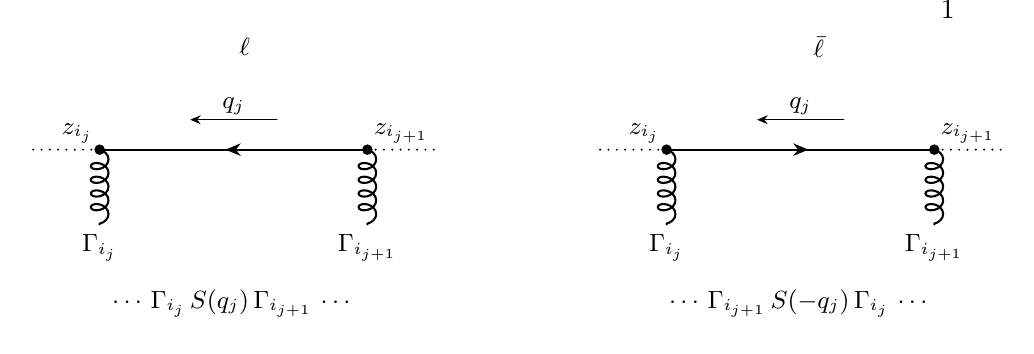
\begin{tikzpicture}[fd]
  \def\fdW{3.4}
  % ---------------- 左：取向 \ell，费米子由 z_{i_{j+1}} 流向 z_{i_j} ----------------
  \begin{scope}
    \coordinate (L) at (0,0); \coordinate (R) at (\fdW,0);
    \draw[line width=0.8pt,dash pattern=on 0pt off 3pt] (L) -- ++(-0.9,0);
    \draw[line width=0.8pt,dash pattern=on 0pt off 3pt] (R) -- ++(0.9,0);
    \draw[quark] (R) -- (L);
    \draw[gluon] (L) -- ++(0,-0.95) coordinate (gL);
    \draw[gluon] (R) -- ++(0,-0.95) coordinate (gR);
    \node[below] at (gL) {$\Gamma_{i_j}$};
    \node[below] at (gR) {$\Gamma_{i_{j+1}}$};
    \node[vertex] at (L) {}; \node[vertex] at (R) {};
    \node[anchor=south east,inner sep=2pt] at (L) {$z_{i_j}$};
    \node[anchor=south west,inner sep=2pt] at (R) {$z_{i_{j+1}}$};
    \path[mom'={$q_j$},mom sep=0.38cm,mom length=1.1cm] (R) -- (L);
    \node at (0.5*\fdW,1.3) {取向 $\ell$};
    \node at (0.5*\fdW,-1.95) {$\cdots\,\Gamma_{i_j}\,S(q_j)\,\Gamma_{i_{j+1}}\,\cdots$};
  \end{scope}
  % ---------------- 右：反向取向 \bar\ell，费米子由 z_{i_j} 流向 z_{i_{j+1}} ----------------
  \begin{scope}[xshift=7.2cm]
    \coordinate (L) at (0,0); \coordinate (R) at (\fdW,0);
    \draw[line width=0.8pt,dash pattern=on 0pt off 3pt] (L) -- ++(-0.9,0);
    \draw[line width=0.8pt,dash pattern=on 0pt off 3pt] (R) -- ++(0.9,0);
    \draw[quark] (L) -- (R);
    \draw[gluon] (L) -- ++(0,-0.95) coordinate (gL);
    \draw[gluon] (R) -- ++(0,-0.95) coordinate (gR);
    \node[below] at (gL) {$\Gamma_{i_j}$};
    \node[below] at (gR) {$\Gamma_{i_{j+1}}$};
    \node[vertex] at (L) {}; \node[vertex] at (R) {};
    \node[anchor=south east,inner sep=2pt] at (L) {$z_{i_j}$};
    \node[anchor=south west,inner sep=2pt] at (R) {$z_{i_{j+1}}$};
    \path[mom'={$q_j$},mom sep=0.38cm,mom length=1.1cm] (R) -- (L);
    \node at (0.5*\fdW,1.3) {反向取向 $\bar\ell$};
    \node at (0.5*\fdW,-1.95) {$\cdots\,\Gamma_{i_{j+1}}\,S(-q_j)\,\Gamma_{i_j}\,\cdots$};
  \end{scope}
\end{tikzpicture}
\caption{镜像动量配置。左：在取向 $\ell$ 中，费米子数由 $z_{i_{j+1}}$ 流向 $z_{i_j}$，这条内线沿箭头的动量为 $q_j$，对应矩阵串中的 $S(q_j)$。右：在反向取向 $\bar\ell$ 中箭头反向，但同一条几何内线携带同一个物理动量（上方的细箭头，方向不变）；沿新的费米子箭头度量，它是 $-q_j$，对应 $S(-q_j)$。矩阵一律逆着费米子箭头读出。}
\label{fig:dirac-mirror}
\end{figure}

\paragraph{另一种证明（只含 $\gamma^\mu$ 顶点）。}当 $\Gamma_j=\gamma^{\mu_j}$ 时，\cref{eq:loop-reversal-mom}可拆成两步，每一步只用到\cref{lem:trace-reversal}与 (T4)，因而在 $D$ 维中同样成立。(a) 反序而动量不变，不产生符号：
\begin{equation}\label{eq:dirac-reversion}
\TrD\bigl[\gamma^{\mu_1}S(q_1)\gamma^{\mu_2}S(q_2)\cdots\gamma^{\mu_k}S(q_k)\bigr]=\TrD\bigl[\gamma^{\mu_1}S(q_k)\gamma^{\mu_k}S(q_{k-1})\cdots\gamma^{\mu_2}S(q_1)\bigr].
\end{equation}
把每个 $S(q_j)$ 的分子展开为 $\sla q_j$ 与 $m$ 两项，左端成为 $\gamma$ 单项式之迹的线性组合；对每个单项式用\cref{eq:trace-reversal}反序，再用循环性把 $\gamma^{\mu_1}$ 移到最前，重新合并即得右端（每个 $S(q)$ 只含 $\mathbb 1$ 与一个 $\gamma$，反序不改变它）。(b) 把全部动量反号，产生 $(-1)^k$：
\begin{equation}\label{eq:dirac-momflip}
\TrD\bigl[\gamma^{\mu_1}S(-q_k)\gamma^{\mu_k}\cdots\gamma^{\mu_2}S(-q_1)\bigr]=(-1)^k\,\TrD\bigl[\gamma^{\mu_1}S(q_k)\gamma^{\mu_k}\cdots\gamma^{\mu_2}S(q_1)\bigr].
\end{equation}
分母是动量的偶函数；展开分子后，恰有 $s$ 个传播子取 $\sla q$ 项的那些项含 $k+s$ 个 $\gamma$，由 (T4) 只有 $s\equiv k\pmod 2$ 的项不为零，而动量反号使它们乘以 $(-1)^s=(-1)^k$。(a)(b) 合起来即 $\Gamma_j=\gamma^{\mu_j}$ 时的\cref{eq:loop-reversal-mom}。这一分解澄清了一个常见的混淆：$(-1)^k$ 并不来自顶点次序的反转（动量标记不变时反序不产生符号），而来自内线动量相对于费米子箭头的反号；因此“反向的圈等于原来的圈乘以 $(-1)^k$”只有在指明动量配置之后才有意义。(T4) 在这里只确定 (b) 中的符号，并不使某个取向单独为零（见\cref{sec:thmI-interpretation}）。

\paragraph{适用范围。}证明只用到 $\TrD\Cconj X=\TrD X$、反自同构性质、$\Cconj{\Gamma_j}=\eta_j\Gamma_j$ 与 $\Cconj{S(q)}=S(-q)$，并且是固定动量（或固定顶点位置）下的代数恒等式。因此：(1) 四维中直接成立。(2) Pauli--Villars：若在传播子层次正规化，$S_{\mathrm{PV}}(q)=\sum_ic_iS(q;M_i)$ 满足 $\Cconj{S_{\mathrm{PV}}(q)}=S_{\mathrm{PV}}(-q)$，证明逐字成立；若把每个闭合圈替换为同一个圈在各质量 $M_i$ 下之值的线性组合 $\sum_ic_i(\cdots)$，则恒等式对每个 $M_i$ 成立，由线性对组合也成立；适当选取 $c_i$ 与 $M_i$（满足若干形如 $\sum_ic_iM_i^s=0$ 的条件，见\cref{sec:reg-pv}）时，两种做法中积分（Wick 转动后）都绝对收敛，从而在平移与反射下不变，动量配置无关紧要。(3) 维数正规化：对 $\Gamma_j\in\{\mathbb 1,\gamma^\mu,\sigma^{\mu\nu}\}$，C~宇称的计算只用到反自同构性质与 $\Cconj{\gamma^\mu}=-\gamma^\mu$，$\Cconj{S(q)}=S(-q)$ 对 $D$ 维动量同样成立，迹的不变性由\cref{lem:trace-reversal}给出；含 $\gamma^5$ 的顶点见\cref{rem:dirac-gamma5}。(4) 一般地，只要满足\cref{def:reg-hypotheses}中的 (R1)，结论就成立（格点情形见\cref{sec:reg-lattice}与\cref{thm:lattice}）。(5) 形如 $a(q)\mathbb 1+b_\mu(q)\gamma^\mu$（$a$ 偶、$b$ 奇）的两点插入（如质量与波函数抵消项）在镜像配置下与一个附加的传播子行为相同；更一般地，依赖于沿箭头的流入、流出动量的顶点 $V(p_{\mathrm{in}},p_{\mathrm{out}})$ 须满足 $\Cconj{V(p_{\mathrm{in}},p_{\mathrm{out}})}=\eta_V\,V(-p_{\mathrm{out}},-p_{\mathrm{in}})$。

\paragraph{短圈。}当 $k\le2$ 时 $\bar\ell=\ell$（\cref{def:loop-factor}），\cref{eq:loop-reversal}不再联系两个不同的缩并，而成为一致性条件 $K_\ell=\bigl(\prod_j\eta_{i_j}\bigr)K_\ell$：若 $\prod_j\eta_{i_j}=-1$，则 $K_\ell=0$。对 $k=1$ 的矢量顶点，这就是蝌蚪图 $\TrD[\gamma^\mu S_{\mathrm{reg}}(0)]=0$（这里 $S_{\mathrm{reg}}(0)$ 是坐标空间传播子在 $x=0$ 处的值；由 (R1)，$\Cconj{S_{\mathrm{reg}}(0)}=S_{\mathrm{reg}}(0)$，故 $\TrD[\gamma^\mu S_{\mathrm{reg}}(0)]=\TrD[\Cconj{S_{\mathrm{reg}}(0)}\,\Cconj{\gamma^\mu}]=-\TrD[\gamma^\mu S_{\mathrm{reg}}(0)]$；等价地，按\cref{rem:dirac-regprop}的记号，$S_{\mathrm{reg}}(x)$ 的 $\gamma^\nu$ 分量 $B_\nu(x):=\tfrac14\TrD[\gamma_\nu S_{\mathrm{reg}}(x)]$ 是奇函数，$B_\nu(0)=0$）。对 $k=2$ 的两个矢量顶点条件是平凡的；对一个矢量顶点与一个标量顶点（$\eta_1\eta_2=-1$），它给出 $\TrD[\gamma^\mu\SF(x)\SF(-x)]=0$，这可以直接验证：$\SF(\pm x)=A(x)\mathbb 1\pm B_\nu(x)\gamma^\nu$，$A=m\Delta_F$ 为偶函数，$B_\nu=\ii\partial_\nu\Delta_F$ 为奇函数，故 $\SF(x)\SF(-x)=(A^2-B_\nu B^\nu)\mathbb 1$（$x\neq0$；未正规化的乘积在 $x=0$ 处不局部可积，那里可能的接触项由正规化决定，参见\cref{eq:reg-mixing}）。对在顶点重合处也有定义且满足 (R1) 的正规化传播子，这些一致性条件对一切顶点位置逐点成立，它们保证了\cref{thm:furry-single}中关于 $k\le2$ 的陈述。在动量空间中，$\bar\ell=\ell$ 的镜像配置只是同一圈积分的重参数化（$k=1$：$q\to-q$；$k=2$，按\cref{eq:dirac-polygon}：$l\to-l-p_2$），\cref{eq:loop-reversal-mom}只说明被积函数在其下乘以 $\prod_j\eta_{i_j}$；$\prod_j\eta_{i_j}=-1$ 时圈积分为零还需要 (R2) 对自反向圈的要求，详见\cref{rem:reg-selfreverse}。

\paragraph{小结。}对 $k$ 个夸克--胶子顶点，$K_{\bar\ell}=(-1)^kK_\ell$，这与 QED 中完全相同。在 QED 中两种取向的电荷因子相同，奇数 $k\ge3$ 的两种取向因而相消（$k=1$ 时 $\bar\ell=\ell$，由上面的一致性条件 $K_\ell=0$），这就是 Furry 的原始定理\cite{Furry1937}（\cref{cor:qed}）。在 QCD 中，反向圈的色因子是反序的色迹，它等于共轭表示的色迹乘以 $(-1)^k$（\cref{lem:color-reversal}）；两个 $(-1)^k$ 如何相消见\cref{thm:furry-single}的证明。

%% ======================================================================
%% 第 4 节  色空间中的电荷共轭
%% ======================================================================
\section{色空间中的电荷共轭}\label{sec:color}

在\cref{sec:dirac}中，电荷共轭在 Dirac 空间中的作用被归结为反自同构 $X\mapsto\Cconj X$，它把闭合夸克圈的 Dirac 因子与其反向圈的 Dirac 因子联系起来（\cref{prop:loop-reversal}）。
本节讨论电荷共轭在色空间中的作用；正是这一部分使 QCD 中的 Furry 定理与 QED 中的原始形式有本质的不同。
由\cref{prop:L-invariance}，规范固定的 QCD 拉氏量在 $A_\mu\to-A_\mu^{\tp}$（连同\cref{eq:C-fields}中其余场的变换）下不变，
因此电荷共轭在伴随色指标上的作用由 Lie 代数自同构 $\varphi(X)=-X^{\tp}$ 诱导的实正交矩阵 $R$ 给出（\cref{def:phi-R}）。本节的主要结论是：
\begin{enumerate}[label=(\arabic*),leftmargin=2.2em]
\item $\delta^{ab}$ 与 $f^{abc}$ 是 C~偶的，$d^{abc}$ 是 C~奇的（\cref{lem:R-properties}）；由 C~偶张量经张量积与缩并构成的色张量是 C~偶的，
因而胶子与鬼场的传播子和顶点（以及 C~不变方案中的抵消项顶点）的色因子都是 C~偶的（\cref{lem:contraction}与\cref{lem:building-blocks}）；
\item 对 $\mathrm{SU}(N)$ 的任意表示 $r$，反序的色迹等于原色迹的复共轭，并且（相差符号 $(-1)^n$）等于共轭表示 $\bar r$ 的色迹 $\tau_{\bar r}=\Rop\tau_r$（\cref{lem:color-reversal}）：
反向的夸克圈就是反夸克圈，夸克圈与其反向圈之和只剩加倍的 C~偶部分 $2\Pp\tau$；
\item $n=3,4$ 时 C~偶与 C~奇部分的显式形式（\cref{prop:n34}）；
\item $\mathrm{SU}(2)$ 与 $\mathrm{SU}(N\ge3)$ 的本质区别（\cref{prop:su2}），以及不超过四个伴随指标的不变张量及其 C~宇称（\cref{lem:invariants}）。
\end{enumerate}
这些都是纯粹的色代数命题，与时空维数、动量配置和正规化方案无关；它们与\cref{sec:dirac}的结果一起，构成\cref{sec:thmI}与\cref{sec:thmII}中证明主定理所需的全部代数输入。
$\mathrm{SU}(3)$ 的显式数据见\cref{app:su3}，较长的色迹计算与 $\mathrm{SU}(N)$ 恒等式的证明见\cref{app:traces}。

%% ----------------------------------------------------------------------
\subsection{\texorpdfstring{$\mathrm{SU}(N)$}{SU(N)} 记号回顾}\label{sec:color-recap}

沿用\cref{sec:setup}的约定。记 $\mathfrak h_N:=\{X\in M_N(\mathbb C):X^\dagger=X,\ \Tr X=0\}$，它是 $N^2-1$ 维实向量空间，$\su(N)=\ii\,\mathfrak h_N$。
生成元 $T^a$（$a=1,\dots,N^2-1$）构成 $\mathfrak h_N$ 的一组基，$\Tr(T^aT^b)=\tfrac12\delta^{ab}$（下文称满足这一归一化的生成元组为正交归一的，即在内积 $2\Tr(X^\dagger Y)$ 下正交归一）。
$N^2$ 个矩阵 $\{\mathbb 1/\sqrt N,\ \sqrt2\,T^a\}$ 在内积 $(X,Y)=\Tr(X^\dagger Y)$ 下正交归一，因而构成 $M_N(\mathbb C)$ 的基，任意复矩阵可展开为
\begin{equation}\label{eq:color-complete}
X=\frac1N\Tr(X)\,\mathbb 1+2\Tr(XT^a)\,T^a ;
\end{equation}
若 $X$ 是 Hermite 矩阵，系数 $2\Tr(XT^a)$ 是实数，因为两个 Hermite 矩阵之积的迹是实数：$\overline{\Tr(XT^a)}=\Tr\bigl((XT^a)^\dagger\bigr)=\Tr(T^aX)$。
按定义 $[T^a,T^b]=\ii f^{abc}T^c$，$\{T^a,T^b\}=\frac1N\delta^{ab}\mathbb 1+d^{abc}T^c$；右乘 $T^c$ 取迹得
\begin{equation}\label{eq:color-fd-traces}
f^{abc}=-2\ii\,\Tr\bigl([T^a,T^b]\,T^c\bigr),\qquad d^{abc}=2\Tr\bigl(\{T^a,T^b\}\,T^c\bigr).
\end{equation}
$f^{abc}$ 实且全反对称，$d^{abc}$ 实且全对称（见\cref{eq:setup-generators}）。把对易关系与反对易关系相加再除以 $2$，得乘积公式
\begin{equation}\label{eq:color-TT}
T^aT^b=\frac{1}{2N}\,\delta^{ab}\,\mathbb 1+\frac12\bigl(d^{abc}+\ii f^{abc}\bigr)T^c .
\end{equation}
伴随表示的生成元为 $(F^a)_{bc}=-\ii f^{abc}$。以下事实的证明见\cref{app:traces}：$[F^a,F^b]=\ii f^{abc}F^c$（Jacobi 恒等式），以及
\begin{equation}\label{eq:color-contractions}
T^aT^a=C_F\mathbb 1,\quad f^{acd}f^{bcd}=N\delta^{ab},\quad d^{acd}d^{bcd}=\frac{N^2-4}{N}\,\delta^{ab},\quad f^{acd}d^{bcd}=0,\quad d^{aab}=0,
\end{equation}
其中 $C_F=\frac{N^2-1}{2N}$；第二式即 $\Tr(F^aF^b)=C_A\delta^{ab}$，$C_A=N$；此外 $T_F=\tfrac12$。

\paragraph{$d^{abc}$ 何时为零。}
对 $X=x^aT^a\in\mathfrak h_N$（$x^a$ 实），由\cref{eq:color-fd-traces}与 $d^{abc}$ 的全对称性，
\begin{equation}\label{eq:color-dxxx}
d^{abc}x^ax^bx^c=2\Tr\bigl(\{X,X\}X\bigr)=4\Tr X^3 .
\end{equation}
全对称张量由其三次型唯一确定，故 $d^{abc}\equiv0$ 当且仅当 $\Tr X^3$ 在 $\mathfrak h_N$ 上恒为零。
$N=2$ 时 $X\in\mathfrak h_2$ 的本征值为 $\pm\lambda$，故 $d^{abc}\equiv0$（亦可由 $\{\sigma^a,\sigma^b\}=2\delta^{ab}\mathbb 1$ 直接看出）；
$N\ge3$ 时取 $X=\mathrm{diag}(1,1,-2,0,\dots,0)$，$\Tr X^3=-6\neq0$，故 $d^{abc}\not\equiv0$。

%% ----------------------------------------------------------------------
\subsection{自同构 \texorpdfstring{$\varphi$}{φ} 与矩阵 \texorpdfstring{$R$}{R}}\label{sec:color-phi}

由\cref{eq:C-fields}，电荷共轭把胶子场 $A_\mu=A_\mu^aT^a$ 变为 $-A_\mu^{\tp}=A^a_\mu\bigl(-(T^a)^{\tp}\bigr)$，所以在色空间中起作用的是映射 $X\mapsto-X^{\tp}$。
简单的符号翻转 $A_\mu\to-A_\mu$ 等价于 $g\to-g$，并不是 Yang--Mills 作用量的对称性（\cref{eq:intro-F}）；
$A_\mu\to-A_\mu^{\tp}$ 之所以可行，是因为 $X\mapsto-X^{\tp}$ 保持对易子（\cref{lem:R-properties}(i)）。

\begin{definition}[色空间中的电荷共轭]\label{def:phi-R}
对 $N\times N$ 复矩阵定义 $\varphi(X)=-X^{\tp}$。由于 $\varphi(T^a)$ 仍是无迹 Hermite 矩阵，可写
\begin{equation}\label{eq:R-def}
\varphi(T^a)=-(T^a)^{\tp}=R^{ab}\,T^b,\qquad R^{ab}=-2\Tr\bigl((T^a)^{\tp}T^b\bigr).
\end{equation}
对带 $n$ 个伴随指标的色张量 $t$（其分量可以取值于任意复向量空间，例如依赖于 Lorentz 指标与时空坐标）定义
$(\Rop_n t)^{a_1\cdots a_n}=R^{a_1b_1}\cdots R^{a_nb_n}\,t^{b_1\cdots b_n}$；在不致混淆时略去下标 $n$。
若 $\Rop t=t$（$\Rop t=-t$），称 $t$ 为 C~偶（C~奇）的。记 $\Pp=\tfrac12(1+\Rop)$，$\Pm=\tfrac12(1-\Rop)$，并对 $\eta=\pm1$ 记 $\mathcal P_\eta=\tfrac12(1+\eta\Rop)$。
\end{definition}

\cref{eq:R-def}中的展开成立，是因为 $\varphi(T^a)\in\mathfrak h_N$：对 Hermite 矩阵 $X$ 有 $(X^{\tp})^\dagger=\overline X=(X^\dagger)^{\tp}=X^{\tp}$，且 $\Tr(-X^{\tp})=-\Tr X$；
于是由\cref{eq:color-complete}，$\varphi(T^a)=2\Tr\bigl(\varphi(T^a)T^b\bigr)T^b=R^{ab}T^b$。
$\Rop_n$ 在每个指标上作用同一个 $R$，因而与指标的任意置换对易，张量的 C~宇称与其指标的书写次序无关；
又因 $\Rop$ 只作用于色指标，以下论证对分量为 Lorentz 张量、坐标或动量的函数乃至 Grassmann 代数元素的色张量逐字成立。

\begin{lemma}[$\varphi$ 与 $R$ 的性质]\label{lem:R-properties}
(i) $\varphi$ 是对易子括号下的 Lie 代数自同构：$\varphi([X,Y])=[\varphi(X),\varphi(Y)]$；$\varphi^2=\mathrm{id}$；$\Tr\bigl(\varphi(X)\varphi(Y)\bigr)=\Tr(XY)$。
(ii) $R$ 是实、对称、正交矩阵，$R^2=\mathbb 1$；因而 $\Rop^2=1$，$\Pp$ 与 $\Pm$ 是互补的投影。
(iii) $\delta^{ab}$ 与 $f^{abc}$ 是 C~偶的，$d^{abc}$ 是 C~奇的：
\begin{equation}\label{eq:f-even-d-odd}
R^{aa'}R^{bb'}\delta^{a'b'}=\delta^{ab},\qquad
R^{aa'}R^{bb'}R^{cc'}f^{a'b'c'}=f^{abc},\qquad
R^{aa'}R^{bb'}R^{cc'}d^{a'b'c'}=-d^{abc}.
\end{equation}
(iv) 在 $\mathrm{SU}(3)$ 的 Gell-Mann 基中，$R=\mathrm{diag}(-1,+1,-1,-1,+1,-1,+1,-1)$。
\end{lemma}

\begin{proof}
\emph{(i)} $\varphi$ 是复线性的。对任意 $N\times N$ 矩阵 $X,Y$，
\begin{align*}
\varphi([X,Y])&=-(XY-YX)^{\tp}=-Y^{\tp}X^{\tp}+X^{\tp}Y^{\tp}=[X^{\tp},Y^{\tp}]=[-X^{\tp},-Y^{\tp}]\\
&=[\varphi(X),\varphi(Y)],\\
\Tr\bigl(\varphi(X)\varphi(Y)\bigr)&=\Tr\bigl(X^{\tp}Y^{\tp}\bigr)=\Tr\bigl((YX)^{\tp}\bigr)=\Tr(YX)=\Tr(XY),
\end{align*}
且 $\varphi(\varphi(X))=-(-X^{\tp})^{\tp}=X$。同样的计算给出
\begin{equation}\label{eq:color-phi-product}
\varphi(XY)=-\varphi(Y)\,\varphi(X),\qquad \varphi\bigl(\{X,Y\}\bigr)=-\bigl\{\varphi(X),\varphi(Y)\bigr\},\qquad\varphi(\mathbb 1)=-\mathbb 1 ,
\end{equation}
即相对于矩阵乘积，$\varphi$ 是带负号的反自同构，被保持的只是对易子。

\emph{(ii)} 实性：$R^{ab}=2\Tr\bigl(\varphi(T^a)T^b\bigr)$ 是两个 Hermite 矩阵之积的迹，因而是实数。
对称性：矩阵与其转置的迹相等，故 $\Tr\bigl((T^a)^{\tp}T^b\bigr)=\Tr\bigl((T^b)^{\tp}T^a\bigr)$。
正交性：由 (i)，$\tfrac12\delta^{ab}=\Tr\bigl(\varphi(T^a)\varphi(T^b)\bigr)=R^{ac}R^{bd}\Tr(T^cT^d)=\tfrac12(RR^{\tp})^{ab}$。
对合性：$T^a=\varphi(\varphi(T^a))=\varphi(R^{ab}T^b)=R^{ab}R^{bc}T^c$，而 $T^c$ 线性无关，故 $R^2=\mathbb 1$。
于是 $\Rop^2=1$，$\Pp^2=\tfrac14(1+2\Rop+\Rop^2)=\Pp$，$\Pm^2=\Pm$，$\Pp\Pm=\tfrac14(1-\Rop^2)=0$，$\Pp+\Pm=1$，$\Rop\Pp=\Pp$，$\Rop\Pm=-\Pm$。

\emph{(iii)} $\delta^{ab}$：$R^{aa'}R^{bb'}\delta^{a'b'}=(RR^{\tp})^{ab}=\delta^{ab}$。
$f^{abc}$：把 $\varphi$ 作用于 $[T^a,T^b]=\ii f^{abc}T^c$。由 (i)，左边为 $[\varphi(T^a),\varphi(T^b)]=\ii R^{aa'}R^{bb'}f^{a'b'c'}T^{c'}$，右边为 $\ii f^{abc}R^{cc'}T^{c'}$；
比较 $T^{c'}$ 的系数得 $R^{aa'}R^{bb'}f^{a'b'c'}=f^{abc}R^{cc'}$，两边乘以 $R^{c''c'}$ 并对 $c'$ 求和（$RR^{\tp}=\mathbb 1$），即得\cref{eq:f-even-d-odd}第二式。
$d^{abc}$：把 $\varphi$ 作用于 $\{T^a,T^b\}=\frac1N\delta^{ab}\mathbb 1+d^{abc}T^c$。由\cref{eq:color-phi-product}，左边为
$-\{\varphi(T^a),\varphi(T^b)\}=-R^{aa'}R^{bb'}\bigl(\frac1N\delta^{a'b'}\mathbb 1+d^{a'b'c'}T^{c'}\bigr)$，右边为 $-\frac1N\delta^{ab}\mathbb 1+d^{abc}R^{cc'}T^{c'}$。
$\{\mathbb 1,T^c\}$ 线性无关：比较 $\mathbb 1$ 的系数只重现 $\delta^{ab}$ 的 C~偶性，比较 $T^{c'}$ 的系数得 $-R^{aa'}R^{bb'}d^{a'b'c'}=d^{abc}R^{cc'}$，同上即得 $\Rop_3d=-d$。
两种符号的来源一目了然：$\varphi$ 保持对易子，却使反对易子反号。

\emph{(iv)} $T^a=\lambda^a/2$（\cref{eq:app-su3-gellmann}）。$\lambda^1,\lambda^3,\lambda^4,\lambda^6,\lambda^8$ 实对称，$\varphi(T^a)=-T^a$；$\lambda^2,\lambda^5,\lambda^7$ 纯虚反对称，$\varphi(T^a)=+T^a$。故 $R$ 是所述对角矩阵（\cref{tab:app-su3-R}）。
\end{proof}

\begin{remark}[与基的选取无关]\label{rem:color-R-spectrum}
$R$ 是 $\varphi|_{\mathfrak h_N}$ 在正交归一基 $\{T^a\}$ 中的矩阵。对 $X\in\mathfrak h_N$ 有 $X^{\tp}=\overline X$，故 $R$ 的 $+1$（$-1$）本征空间由纯虚反对称（实对称）的 $X\in\mathfrak h_N$ 组成，
其维数为 $\frac12N(N-1)$（$\frac12(N-1)(N+2)$），见\cref{tab:app-su3-suN}。换用另一组正交归一生成元 $T'^a=O^{ab}T^b$（$O$ 实正交）时 $R'=ORO^{\tp}$，
且 $\Rop'(O^{\otimes n}t)=O^{\otimes n}(\Rop t)$，所以“C~偶”“C~奇”与基无关。
$R$ 在一组正交归一基中是对角的，当且仅当每个基元都是实对称或纯虚反对称的（例如广义 Gell-Mann 基，\cref{sec:app-su3-suN}）；在一般的正交归一基中 $R$ 不是对角的。
$\det R=(-1)^{(N-1)(N+2)/2}$ 不能用来判别 $\varphi$ 是否为内自同构：$N=5$ 时 $\det R=+1$，但 $\varphi$ 是外自同构（\cref{prop:su2}）。
\end{remark}

\begin{remark}[$\varphi$ 是复共轭的微分]\label{rem:color-group}
对 $g=\ee^{\ii\alpha^aT^a}\in\mathrm{SU}(N)$（$\alpha^a$ 实），由 $\overline{T^a}=(T^a)^{\tp}$ 得
\begin{equation}\label{eq:color-conj-group}
\overline g=\ee^{-\ii\alpha^a\overline{T^a}}=\ee^{\ii\alpha^a\varphi(T^a)}=\ee^{\ii\alpha^aR^{ab}T^b}.
\end{equation}
复共轭 $\Phi(g):=\overline g$ 是 $\mathrm{SU}(N)$ 的连续自同构，而 $\varphi$ 在 $\su(N)$ 上恰是它的微分（对反 Hermite 的 $Y$，$\varphi(Y)=-Y^{\tp}=\overline Y$）；
这正是格点上 $U_{x,\mu}\mapsto\overline{U_{x,\mu}}$（\cref{thm:lattice}）在连续统中的对应。在胶子场上 $A^a_\mu\mapsto R^{ab}A^b_\mu$（$R$ 对称），
而由 $\varphi$ 的线性与\cref{lem:R-properties}(i)，$F_{\mu\nu}[\varphi(A)]=\varphi(F_{\mu\nu}[A])$，即 $F^a_{\mu\nu}\mapsto R^{ab}F^b_{\mu\nu}$（详见\cref{prop:L-invariance}的证明）。
\end{remark}

%% ----------------------------------------------------------------------
\subsection{色张量的 C~宇称与 Feynman 规则的构件}\label{sec:color-parity}

\begin{lemma}[C~宇称的乘法性与正交性]\label{lem:contraction}
(i) 若色张量 $s,t$ 的 C~宇称分别为 $\epsilon_s,\epsilon_t\in\{\pm1\}$，则 $s\otimes t$ 及其对任意一对指标（用 $\delta^{ab}$）的缩并的 C~宇称为 $\epsilon_s\epsilon_t$。
(ii) 对 $n$ 指标张量定义双线性型 $\langle s,t\rangle=s^{a_1\cdots a_n}t^{a_1\cdots a_n}$，则 $\langle\Rop s,\Rop t\rangle=\langle s,t\rangle$；因而 C~宇称相反的两个张量正交。
(iii) 由 $\delta^{ab}$ 与 $f^{abc}$ 经张量积与缩并构成的任何色张量都是 C~偶的；特别地，伴随表示的迹 $\Tr(F^{a_1}\cdots F^{a_n})$（$(F^a)_{bc}=-\ii f^{abc}$）是 C~偶的。
\end{lemma}

\begin{proof}
\emph{(i)} 按定义 $\Rop$ 在每个指标上作用一个 $R$，故 $\Rop_{n+m}(s\otimes t)=(\Rop_ns)\otimes(\Rop_mt)=\epsilon_s\epsilon_t\,s\otimes t$。
设 $u$ 为 $n$ 指标张量，$\mathsf k_{pq}u$ 为把其第 $p$、$q$ 个指标用 $\delta$ 缩并所得的张量，$(\mathsf k_{pq}u)^{\cdots}=u^{\cdots e\cdots e\cdots}$。只写出第 $p$、$q$ 个指标上的 $R$，
\[
\mathsf k_{pq}(\Rop_nu)=\cdots R^{eb_p}R^{eb_q}\cdots u^{\cdots b_p\cdots b_q\cdots}=\cdots\bigl(R^{\tp}R\bigr)^{b_pb_q}\cdots u^{\cdots b_p\cdots b_q\cdots}=\Rop_{n-2}(\mathsf k_{pq}u),
\]
这里用了 $R^{\tp}R=\mathbb 1$。所以缩并与 $\Rop$ 对易：若 $\Rop u=\epsilon u$，则 $\Rop(\mathsf k_{pq}u)=\epsilon\,\mathsf k_{pq}u$。取 $u=s\otimes t$ 即得 (i)。

\emph{(ii)} 由 $R^{\tp}R=\mathbb 1$，$\langle\Rop s,\Rop t\rangle=\prod_{i=1}^n\bigl(R^{\tp}R\bigr)^{b_ic_i}\,s^{b_1\cdots b_n}t^{c_1\cdots c_n}=\langle s,t\rangle$。
若 $\Rop s=s$、$\Rop t=-t$，则 $\langle s,t\rangle=\langle\Rop s,\Rop t\rangle=-\langle s,t\rangle=0$。
$\langle\cdot,\cdot\rangle$ 是双线性而非半双线性的，因而对复值或取值于向量空间的张量同样适用。

\emph{(iii)} 由 (i) 与\cref{lem:R-properties}(iii) 对构造步骤归纳即得；指标重排不改变 C~宇称。伴随表示的迹是 $f^{abc}$ 的网络，
\begin{equation}\label{eq:color-adjoint-trace}
\Tr\bigl(F^{a_1}F^{a_2}\cdots F^{a_n}\bigr)=(-\ii)^n\,f^{a_1x_1x_2}f^{a_2x_2x_3}\cdots f^{a_nx_nx_1},
\end{equation}
因而是 C~偶的。
\end{proof}

由\cref{lem:contraction}(ii) 还可知 $\Rop$ 关于 $\langle\cdot,\cdot\rangle$ 自伴：$\langle\Rop s,t\rangle=\langle\Rop s,\Rop^2t\rangle=\langle s,\Rop t\rangle$。
因此 $\Pp,\Pm$ 是正交投影，并且对任意 $G$ 与 C~奇张量 $t$ 有 $\langle t,G\rangle=\langle t,\Pm G\rangle$；这是\cref{cor:selection}(a) 的代数基础。

\begin{lemma}[Feynman 规则其余构件的 C~偶性]\label{lem:building-blocks}
胶子与鬼场传播子的色因子 $\delta^{ab}$，三胶子顶点与鬼场--胶子顶点的色因子 $f^{abc}$，以及四胶子顶点的三个色结构
$f^{abe}f^{cde}$、$f^{ace}f^{bde}$、$f^{ade}f^{bce}$ 都是 C~偶的；任何 C~不变的重整化方案中的抵消项顶点亦然。
\end{lemma}

\begin{proof}
在\cref{fig:feynman-rules}中，胶子传播子（任意 $\xi$）与鬼场传播子的色因子为 $\delta^{ab}$；三胶子顶点与鬼场--胶子顶点为 $f^{abc}$ 乘以与色无关的 Lorentz 结构；
四胶子顶点是三项之和，每项为一个色结构（$f^{abe}f^{cde}$、$f^{ace}f^{bde}$ 或 $f^{ade}f^{bce}$）乘以与色无关的 Lorentz 张量。
由\cref{lem:R-properties}(iii)，$\delta^{ab}$ 与 $f^{abc}$ 是 C~偶的；$f^{abe}f^{cde}$ 是张量积 $f^{abe}f^{cde'}$ 对指标对 $(e,e')$ 的缩并，由\cref{lem:contraction}(i) 是 C~偶的，另两个结构由它重排指标得到，亦然。

所谓 C~不变的重整化方案，是指抵消项拉氏量本身在\cref{eq:C-fields}下不变。在 $\overline{\mathrm{MS}}$ 等乘法重整化方案中，规范场与鬼场部分的抵消项是 $(Z_i-1)$ 乘以原拉氏量中的单项式，
色张量仍是 $\delta^{ab}$、$f^{abc}$ 或 $f^{abe}f^{cde}$ 型的，故 C~偶。更一般地，设局域泛函 $S_{\mathrm{ct}}[A,c,\bar c]$ 在 $(A,c,\bar c)\mapsto(RA,Rc,R\bar c)$ 下不变，其 $n$ 点顶点函数为
$V^{a_1\cdots a_n}(\dots):=\delta^nS_{\mathrm{ct}}/\delta\Upsilon_1^{a_1}\cdots\delta\Upsilon_n^{a_n}\big|_{\Upsilon=0}$（$\Upsilon_i\in\{A_\mu(x),c(x),\bar c(x)\}$，省略号代表 Lorentz 指标与坐标）。
对 $S_{\mathrm{ct}}[R\Upsilon]=S_{\mathrm{ct}}[\Upsilon]$ 求 $n$ 次泛函导数并令 $\Upsilon=0$，由链式法则（$R$ 为常数实矩阵，对 Grassmann 场的左导数同样适用）得
\begin{equation}\label{eq:color-vertex-invariance}
R^{b_1a_1}\cdots R^{b_na_n}\,V^{b_1\cdots b_n}(\dots)=V^{a_1\cdots a_n}(\dots),
\end{equation}
因 $R$ 对称，这正是 $\Rop V=V$。把同一论证用于 QCD 作用量本身（\cref{prop:L-invariance}）即得上面逐项验证的另一证明；
传播子是二次型 $K$ 之逆，由 $RKR=K$ 知其逆亦然。
\end{proof}

在不含外夸克场的 Green 函数中（\cref{thm:furry-allorders}的情形），夸克线上的构件（夸克传播子 $\delta_{ij}$、夸克--胶子顶点 $T^a$、夸克线抵消项 $\mathbb 1$ 或 $T^a$）都位于闭合夸克圈上，
其色矩阵按\cref{def:loop-factor}组合成圈的色迹，单独谈论其 C~宇称没有意义（开放夸克线见\cref{rem:thmI-open-lines}与\cref{rem:thmII-scope}）；
对它们起作用的是下面的\cref{lem:color-reversal}与主定理 I（\cref{thm:furry-single}），夸克线抵消项的 Dirac 结构见\cref{prop:reg-dimreg}与\cref{eq:thmII-X}。

%% ----------------------------------------------------------------------
\subsection{色迹的反序与共轭表示}\label{sec:color-reversal}

由\cref{def:loop-factor}，夸克圈 $\ell=(i_1\,i_2\cdots i_k)$ 的色因子是 $\tau_\ell=\Tr(T^{a_{i_1}}T^{a_{i_2}}\cdots T^{a_{i_k}})$；
由\cref{eq:setup-reversed}，反向圈 $\bar\ell=(i_1\,i_k\cdots i_2)$ 的色因子 $\tau_{\bar\ell}$ 是原色迹的\emph{反序}迹。下述引理对 $\mathrm{SU}(N)$ 的任意表示刻画反序迹，因而也适用于其他表示中的费米子以及伴随表示。

\begin{lemma}[色迹的反序：任意表示]\label{lem:color-reversal}
设 $r$ 为 $\mathrm{SU}(N)$ 的任一有限维酉表示，生成元为 $T_r^a$；其共轭表示 $\bar r$ 的生成元为 $T_{\bar r}^a=-(T_r^a)^{\tp}$。
记 $\tau_r^{a_1\cdots a_n}=\Tr\bigl(T_r^{a_1}\cdots T_r^{a_n}\bigr)$。则
\begin{equation}\label{eq:color-reversal}
\Tr\bigl(T_r^{a_n}\cdots T_r^{a_1}\bigr)=\overline{\tau_r^{a_1\cdots a_n}}=(-1)^n\,\tau_{\bar r}^{a_1\cdots a_n},
\qquad \tau_{\bar r}=\Rop\,\tau_r .
\end{equation}
因此 Furry 组合
\begin{equation}\label{eq:bracket}
\begin{aligned}
B_r^{a_1\cdots a_n}&:=\tau_r^{a_1\cdots a_n}+(-1)^n\,\Tr\bigl(T_r^{a_n}\cdots T_r^{a_1}\bigr)=\tau_r+\tau_{\bar r}=2\,(\Pp\tau_r)^{a_1\cdots a_n}\\
&\phantom{:}=\begin{cases}2\Real\tau_r^{a_1\cdots a_n}, & n\ \text{为偶数},\\[2pt] 2\ii\,\Imag\tau_r^{a_1\cdots a_n}, & n\ \text{为奇数}.\end{cases}
\end{aligned}
\end{equation}
若 $r\simeq\bar r$（实表示或赝实表示，例如伴随表示以及 $\mathrm{SU}(2)$ 的一切表示），则 $\tau_r$ 对一切 $n$ 都是 C~偶的。
基础表示 $F$ 简记 $\tau=\tau_F$，$B=B_F$。
\end{lemma}

这里有限维酉表示 $r$ 指连续群同态 $r:\mathrm{SU}(N)\to\mathrm U(\dim r)$，生成元由 $r(\ee^{\ii\alpha^aT^a})=\ee^{\ii\alpha^aT_r^a}$ 定义，是满足 $[T_r^a,T_r^b]=\ii f^{abc}T_r^c$ 的 Hermite 矩阵；
记 $\dd r$ 为线性映射 $x^aT^a\mapsto x^aT_r^a$（即 $r$ 的微分，$\dd F=\mathrm{id}$），$\chi_r(g)=\Tr r(g)$ 为特征标。共轭表示 $\bar r(g):=\overline{r(g)}$（因 $r(g)$ 酉，它也就是对偶表示 $g\mapsto r(g^{-1})^{\tp}$）；
由 $\overline{\ee^{\ii\alpha^aT_r^a}}=\ee^{\ii\alpha^a(-(T_r^a)^{\tp})}$，其生成元正是 $T_{\bar r}^a=-(T_r^a)^{\tp}$，特征标为 $\chi_{\bar r}=\overline{\chi_r}$。证明需要下面这个初等事实。

\begin{lemma}\label{lem:color-conjugacy}
对每个 $g\in\mathrm{SU}(N)$，存在 $W\in\mathrm{SU}(N)$ 使 $\overline g=W\,g^{-1}\,W^{-1}$。因而对 $\mathrm{SU}(N)$ 的任一有限维酉表示 $r$，$\chi_r(\overline g)=\overline{\chi_r(g)}=\chi_{\bar r}(g)$。
\end{lemma}

\begin{proof}
由谱定理，$g=VDV^\dagger$，$V$ 酉，$D$ 为对角酉矩阵；以 $\ee^{\ii\theta}V$（$\ee^{\ii N\theta}\det V=1$）代替 $V$ 不改变 $VDV^\dagger$，故可设 $V\in\mathrm{SU}(N)$。
于是 $\overline g=\overline V\,\overline D\,V^{\tp}$，$g^{-1}=V\,\overline D\,V^\dagger$。令 $W:=\overline V\,V^\dagger$，则 $W$ 酉，$\det W=\overline{\det V}\cdot\overline{\det V}=1$，$W^{-1}=W^\dagger=VV^{\tp}$，并且
$W\,g^{-1}\,W^{-1}=\overline V\,V^\dagger\cdot V\overline DV^\dagger\cdot VV^{\tp}=\overline V\,\overline D\,V^{\tp}=\overline g$。
特征标是类函数，$r$ 是酉表示，故 $\chi_r(\overline g)=\chi_r(g^{-1})=\Tr\bigl(r(g)^\dagger\bigr)=\overline{\chi_r(g)}$。
\end{proof}

\begin{proof}[\cref{lem:color-reversal}的证明]
\emph{第一步（Hermite 性）。}由 $\overline{\Tr X}=\Tr X^\dagger$ 与 $(T_r^a)^\dagger=T_r^a$，
\[
\overline{\tau_r^{a_1\cdots a_n}}=\Tr\bigl((T_r^{a_1}\cdots T_r^{a_n})^\dagger\bigr)=\Tr\bigl(T_r^{a_n}\cdots T_r^{a_1}\bigr).
\]

\emph{第二步（转置）。}矩阵与其转置的迹相等，故
\[
\Tr\bigl(T_r^{a_n}\cdots T_r^{a_1}\bigr)=\Tr\bigl((T_r^{a_n}\cdots T_r^{a_1})^{\tp}\bigr)=\Tr\bigl((T_r^{a_1})^{\tp}\cdots(T_r^{a_n})^{\tp}\bigr)=(-1)^n\,\tau_{\bar r}^{a_1\cdots a_n}.
\]
这证明了\cref{eq:color-reversal}的第一串等式。$T_{\bar r}^a$ 满足同一 Lie 代数：$[T_{\bar r}^a,T_{\bar r}^b]=-\bigl([T_r^a,T_r^b]\bigr)^{\tp}=\ii f^{abc}T_{\bar r}^c$。

\emph{第三步（$\Rop\tau_r=\tau_{\bar r}$：基础表示）。}$T_{\bar F}^a=-(T^a)^{\tp}=\varphi(T^a)=R^{ab}T^b$，故
\[
\tau_{\bar F}^{a_1\cdots a_n}=\Tr\bigl(R^{a_1b_1}T^{b_1}\cdots R^{a_nb_n}T^{b_n}\bigr)=(\Rop\tau_F)^{a_1\cdots a_n}.
\]

\emph{第四步（$\Rop\tau_r=\tau_{\bar r}$：一般表示）。}由 $\dd r$ 的线性，$R^{ab}T_r^b=\dd r\bigl(\varphi(T^a)\bigr)$，因此
\begin{equation}\label{eq:color-Rtau-r}
(\Rop\tau_r)^{a_1\cdots a_n}=\Tr\Bigl(\dd r\bigl(\varphi(T^{a_1})\bigr)\cdots\dd r\bigl(\varphi(T^{a_n})\bigr)\Bigr).
\end{equation}
由\cref{eq:color-conj-group}，$r\bigl(\overline{\ee^{\ii\alpha^aT^a}}\bigr)=\ee^{\ii\alpha^a\,\dd r(\varphi(T^a))}$，所以\cref{eq:color-Rtau-r}是“扭曲表示” $r\circ\Phi:g\mapsto r(\overline g)$ 的色迹。
$r\circ\Phi$ 是连续酉表示，由\cref{lem:color-conjugacy}，其特征标 $\chi_r(\overline g)$ 等于 $\chi_{\bar r}(g)$。
紧群的有限维连续表示在等价意义下由其特征标唯一确定（由完全可约性与不可约特征标的 Schur 正交关系，特征标决定每个不可约成分的重数），
故存在可逆矩阵 $U$ 使 $r(\overline g)=U\,\bar r(g)\,U^{-1}$ 对一切 $g$ 成立。取 $g=\ee^{\ii tX}$（$X\in\mathfrak h_N$，$t\in\mathbb R$），
左边为 $\ee^{\ii t\,\dd r(\varphi(X))}$，右边为 $U\,\overline{\ee^{\ii t\,\dd r(X)}}\,U^{-1}=U\ee^{\ii t\,\dd\bar r(X)}U^{-1}$（$\dd\bar r(X)=-\dd r(X)^{\tp}$）；在 $t=0$ 处求导得
$\dd r(\varphi(T^a))=U\,T_{\bar r}^a\,U^{-1}$。代入\cref{eq:color-Rtau-r}，$U$ 在迹中消去，即得 $\Rop\tau_r=\tau_{\bar r}$。

\emph{第五步（Furry 组合）。}由第二、四步，$B_r=\tau_r+\tau_{\bar r}=\tau_r+\Rop\tau_r=2\Pp\tau_r$；由第一步，$B_r=\tau_r+(-1)^n\overline{\tau_r}$，$n$ 偶时为 $2\Real\tau_r$，$n$ 奇时为 $2\ii\Imag\tau_r$。

\emph{第六步（自共轭表示）。}若 $T_{\bar r}^a=U'T_r^aU'^{-1}$，则 $\tau_{\bar r}=\tau_r$，从而 $\Rop\tau_r=\tau_r$。伴随表示满足 $-(F^a)^{\tp}=F^a$（$f^{abc}$ 全反对称），是实表示。
对 $\mathrm{SU}(2)$，直接验证可知 $\overline g=(\ii\sigma^2)g(\ii\sigma^2)^{-1}$（取 $g=\bigl(\begin{smallmatrix}\alpha&\beta\\-\bar\beta&\bar\alpha\end{smallmatrix}\bigr)$；这是\cref{prop:su2}(i) 在群上的形式），
故对任一表示 $r$，$r\circ\Phi(g)=r(\ii\sigma^2)\,r(g)\,r(\ii\sigma^2)^{-1}$，即 $r\circ\Phi\simeq r$；与第四步的 $r\circ\Phi\simeq\bar r$ 合起来得 $\bar r\simeq r$。
\end{proof}

文献中常把\cref{eq:bracket}写成“偶数个顶点的费米子圈给出 $\Real\Tr$，奇数个给出 $\ii\Imag\Tr$”\cite{PastonProkhvatilovFranke1999}；
把它与 C~宇称投影 $\Pp$ 及共轭表示联系起来，正是推广到任意阶（\cref{sec:thmII}）所需要的形式。

\begin{remark}[夸克圈与反夸克圈]\label{rem:color-antiquark}
电荷共轭场 $\psi^{\mathsf c}=C\bar\psi^{\tp}$ 在规范变换 $\psi\to U\psi$ 下按 $\psi^{\mathsf c}\to\overline U\psi^{\mathsf c}$ 变换，即属于 $\bar F$。
由\cref{eq:color-reversal}，$\tau_{\bar\ell}=(-1)^k\tau_{\bar F}^{a_{i_1}\cdots a_{i_k}}$；结合 $K_{\bar\ell}=(-1)^kK_\ell$（\cref{prop:loop-reversal}），这正是\cref{eq:master}的色内容：
\emph{反向的夸克圈等于沿原取向运行的反夸克圈}（参见\cite[第~3~节]{MooreGorda2023}）。
场论解释及与 QED 的对比见\cref{sec:thmI-interpretation}。
\end{remark}

\begin{proposition}[$n=3,4$ 的显式分解]\label{prop:n34}
对基础表示，
\begin{gather}
\tau^{abc}=\tfrac14\bigl(d^{abc}+\ii f^{abc}\bigr),\qquad (\Pp\tau)^{abc}=\tfrac{\ii}{4}f^{abc},\qquad (\Pm\tau)^{abc}=\tfrac14d^{abc},\label{eq:trace3}\\
\tau^{abcd}=\tfrac{1}{4N}\delta^{ab}\delta^{cd}+\tfrac18\bigl(d^{abe}+\ii f^{abe}\bigr)\bigl(d^{cde}+\ii f^{cde}\bigr),\label{eq:trace4}\\
(\Pp\tau)^{abcd}=\tfrac{1}{4N}\delta^{ab}\delta^{cd}+\tfrac18\bigl(d^{abe}d^{cde}-f^{abe}f^{cde}\bigr),\qquad
(\Pm\tau)^{abcd}=\tfrac{\ii}{8}\bigl(d^{abe}f^{cde}+f^{abe}d^{cde}\bigr).\label{eq:P-trace4}
\end{gather}
\end{proposition}

\begin{proof}
$n=3$：把\cref{eq:color-TT}右乘 $T^c$ 取迹，由 $\Tr T^c=0$ 与 $\Tr(T^eT^c)=\frac12\delta^{ec}$，
$\tau^{abc}=\frac12\bigl(d^{abe}+\ii f^{abe}\bigr)\cdot\frac12\delta^{ec}=\frac14\bigl(d^{abc}+\ii f^{abc}\bigr)$。
由\cref{lem:R-properties}(iii) 与 $\Pp,\Pm$ 的线性，$(\Pp\tau)^{abc}=\frac{\ii}{4}f^{abc}$，$(\Pm\tau)^{abc}=\frac14d^{abc}$；作为检验，$B=2\Pp\tau=2\ii\Imag\tau$，与\cref{eq:bracket}一致。
$n=4$：把 $T^aT^b$ 与 $T^cT^d$ 都按\cref{eq:color-TT}展开后相乘取迹即得\cref{eq:trace4}（细节见\cref{app:traces}）。展开乘积，
$\bigl(d^{abe}+\ii f^{abe}\bigr)\bigl(d^{cde}+\ii f^{cde}\bigr)=d^{abe}d^{cde}-f^{abe}f^{cde}+\ii\bigl(d^{abe}f^{cde}+f^{abe}d^{cde}\bigr)$；
由\cref{lem:contraction}(i)，$\delta^{ab}\delta^{cd}$、$d^{abe}d^{cde}$、$f^{abe}f^{cde}$ 是 C~偶的，$d^{abe}f^{cde}$ 与 $f^{abe}d^{cde}$ 是 C~奇的，由此读出\cref{eq:P-trace4}。
$\Pm\tau$ 按三个配对写出的形式（\cref{eq:app-traces-Pm-sym}）等其他形式见\cref{app:traces}。
\end{proof}

由\cref{eq:trace3}，$k=3$ 的 Furry 组合为 $B^{abc}=\tau^{abc}-\tau^{cba}=\Tr(T^a[T^b,T^c])=\frac{\ii}2f^{abc}$：两种取向中正比于 $\frac14d^{abc}$ 的部分严格相消，正比于 $\frac{\ii}4f^{abc}$ 的部分相加
（参见\cite{BlumAlkoferHuberWindisch2015}；这是\cref{cor:three-four}与\cref{prop:triangle}的色代数基础）。

\begin{remark}[一般表示与反常系数]\label{rem:color-anomaly}
设 $N\ge3$，$r$ 为任一有限维酉表示。$\Tr(T_r^aT_r^b)$ 与全对称的 $\Tr\bigl(T_r^a\{T_r^b,T_r^c\}\bigr)$ 是不变张量（\cref{sec:color-invariants}），由\cref{lem:invariants}分别正比于 $\delta^{ab}$ 与 $d^{abc}$。
据此定义 Dynkin 指标 $T(r)$ 与反常系数 $A(r)$：
\begin{equation}\label{eq:color-anomaly-def}
\Tr\bigl(T_r^aT_r^b\bigr)=T(r)\,\delta^{ab},\qquad\Tr\bigl(T_r^a\{T_r^b,T_r^c\}\bigr)=\tfrac12A(r)\,d^{abc}.
\end{equation}
把 $T_r^bT_r^c=\frac12[T_r^b,T_r^c]+\frac12\{T_r^b,T_r^c\}$ 左乘 $T_r^a$ 取迹，得
\begin{equation}\label{eq:color-tau3-r}
\tau_r^{abc}=\frac{\ii}{2}T(r)\,f^{abc}+\frac14A(r)\,d^{abc},\qquad(\Pp\tau_r)^{abc}=\frac{\ii}{2}T(r)\,f^{abc},\qquad(\Pm\tau_r)^{abc}=\frac{A(r)}4\,d^{abc}.
\end{equation}
由\cref{eq:trace3}，$T(F)=\frac12$，$A(F)=1$；由 $\tau_{\bar r}=\Rop\tau_r$ 得 $A(\bar r)=-A(r)$，故自共轭（实或赝实）表示有 $A=0$。由\cref{eq:color-tau3-r}与\cref{eq:color-dxxx}，$\Tr\bigl[\dd r(X)^3\bigr]=A(r)\Tr X^3$。
设 $X$ 的本征值为 $x_1,\dots,x_N$（$\sum_ix_i=0$），$p_3:=\sum_ix_i^3$；则 $\sum_{i,j}(x_i+x_j)^3=2Np_3$，从而 $\sum_{i<j}(x_i+x_j)^3=(N-4)p_3$，$\sum_{i\le j}(x_i+x_j)^3=(N+4)p_3$。
这两者分别是 $r=\Lambda^2F$ 与 $r=\mathrm{Sym}^2F$ 时 $\dd r(X)^3$ 的迹，于是
\begin{equation}\label{eq:color-A-values}
A(F)=1,\quad A(\bar F)=-1,\quad A(\mathrm{adj})=0,\quad A(\mathrm{Sym}^2F)=N+4,\quad A(\Lambda^2F)=N-4 .
\end{equation}
$k=3$ 时 Furry 定理对表示 $r$ 的内容是：两种取向的 C~奇部分 $\frac14A(r)d^{abc}$ 与 $\frac14A(\bar r)d^{abc}$ 相消，即 $A(r)+A(\bar r)=0$；存活的是 $B_r=\ii\,T(r)f^{abc}$。
这与矢量型理论中规范反常相消所用的是同一个群论等式（Dirac 费米子的左手分量属于 $r$，右手分量的共轭属于 $\bar r$），但两者是不同的命题：
反常是含 $\gamma^5$ 的三角图的紫外效应，关乎流的守恒；Furry 相消涉及不含 $\gamma^5$ 的 VVV 圈，在被积函数层次上成立（\cref{prop:triangle}），且不要求费米子内容满足任何反常相消条件。
最后，手征耦合没有确定的 C~宇称（\cref{sec:dirac-parity}），因此这里的 Furry 定理不适用于手征规范理论（例如电弱相互作用）。
\end{remark}

%% ----------------------------------------------------------------------
\subsection{\texorpdfstring{$N=2$ 与 $N\ge3$}{N=2 与 N≥3} 的区别；伴随表示的不变张量}\label{sec:color-invariants}

称 $n$ 指标色张量 $t$ 是（整体 $\mathrm{SU}(N)$）不变的，若对一切 $g\in\mathrm{SU}(N)$，
\begin{equation}\label{eq:color-invariance}
(\mathrm{Ad}_g)^{a_1b_1}\cdots(\mathrm{Ad}_g)^{a_nb_n}\,t^{b_1\cdots b_n}=t^{a_1\cdots a_n},\qquad (\mathrm{Ad}_g)^{ab}:=2\Tr\bigl(T^a\,gT^bg^{-1}\bigr),
\end{equation}
这里 $gT^bg^{-1}=(\mathrm{Ad}_g)^{ab}T^a$；$\mathrm{Ad}_g$ 保持 $\Tr(XY)$，因而是实正交矩阵。设 $r$ 为任一表示，$X\in\mathfrak h_N$。把恒等式
$r(g)\,r(\ee^{\ii sX})\,r(g)^{-1}=r\bigl(\ee^{\ii s\,gXg^{-1}}\bigr)$ 在 $s=0$ 处求导，得
\[
r(g)\,\dd r(X)\,r(g)^{-1}=\dd r(gXg^{-1}),\qquad\text{从而}\qquad r(g)\,T_r^b\,r(g)^{-1}=(\mathrm{Ad}_g)^{ab}\,T_r^a ;
\]
代入色迹并利用 $\mathrm{Ad}_g^{\tp}=\mathrm{Ad}_{g^{-1}}$，即知 $\tau_r$ 是不变张量。$\delta^{ab}$、$f^{abc}$、$d^{abc}$ 是这种迹的线性组合（\cref{eq:color-fd-traces}），亦是不变张量。

\begin{proposition}[$N=2$ 与 $N\ge3$ 的区别]\label{prop:su2}
(i) 对 $\mathrm{SU}(2)$，在无迹矩阵上 $\varphi(X)=(\ii\sigma^2)X(\ii\sigma^2)^{-1}$，即 $\varphi|_{\su(2)}$ 是内自同构，$R=\mathrm{Ad}_{\ii\sigma^2}\in\mathrm{Ad}\bigl(\mathrm{SU}(2)\bigr)$（在 Pauli 基 $T^a=\sigma^a/2$ 中 $R=\mathrm{diag}(-1,+1,-1)$）；
因而每个 $\mathrm{SU}(2)$ 不变张量都是 C~偶的，并且 $\Rop\tau=\tau$，即 $\Tr(T^{a_1}\cdots T^{a_n})=(-1)^n\Tr(T^{a_n}\cdots T^{a_1})$。
(ii) 对 $N\ge3$，$\varphi$ 不是内自同构：内自同构保持 $d^{abc}$ 不变，而 $\Rop d=-d\neq d$。
\end{proposition}

\begin{proof}
\emph{(i)} $\sigma^1,\sigma^3$ 实对称，$\sigma^2$ 纯虚反对称；又 $\sigma^2$ 与 $\sigma^1,\sigma^3$ 反对易且 $(\sigma^2)^2=\mathbb 1$，故 $\sigma^2\sigma^a\sigma^2=-(\sigma^a)^{\tp}$（$a=1,2,3$）。
由 $\ii\sigma^2=\bigl(\begin{smallmatrix}0&1\\-1&0\end{smallmatrix}\bigr)\in\mathrm{SU}(2)$，$(\ii\sigma^2)^{-1}=-\ii\sigma^2$ 及线性，对一切 $2\times2$ 无迹矩阵 $X$（它们由 $\sigma^a$ 复线性张成，
特别是 $X\in\mathfrak h_2$）有 $\varphi(X)=\sigma^2X\sigma^2=(\ii\sigma^2)X(\ii\sigma^2)^{-1}$；而 $\varphi(\mathbb 1)=-\mathbb 1$，故这一等式只在无迹矩阵上成立。
于是在任意正交归一基中 $R^{ab}=2\Tr\bigl(\varphi(T^a)T^b\bigr)=2\Tr\bigl(T^b\,(\ii\sigma^2)T^a(\ii\sigma^2)^{-1}\bigr)=(\mathrm{Ad}_{\ii\sigma^2})^{ba}$；
$\mathrm{Ad}_{\ii\sigma^2}$ 是正交矩阵，又由 $(\ii\sigma^2)^2=-\mathbb 1$ 知它是对合，因而对称，故 $R=\mathrm{Ad}_{\ii\sigma^2}$。
特别地，取 $T^a=\sigma^a/2$，则 $\varphi(T^1)=-T^1$，$\varphi(T^2)=T^2$，$\varphi(T^3)=-T^3$，即 $R=\mathrm{diag}(-1,+1,-1)$（绕第 2 轴转动 $\pi$）。
若 $t$ 是 $\mathrm{SU}(2)$ 不变张量，在\cref{eq:color-invariance}中取 $g=\ii\sigma^2$ 即得 $\Rop t=t$。$\tau$ 是不变张量，故 $\Rop\tau=\tau$；
代入\cref{eq:color-reversal}，$\Tr(T^{a_n}\cdots T^{a_1})=(-1)^n\Rop\tau=(-1)^n\tau$。

\emph{(ii)} 设 $N\ge3$，并设有可逆矩阵 $V$ 使 $\varphi(X)=VXV^{-1}$ 对一切 $X\in\mathfrak h_N$ 成立（这一假设弱于“$\varphi=\mathrm{Ad}_g$，$g\in\mathrm{SU}(N)$”，所得结论因而更强）。由\cref{eq:color-fd-traces}，
\[
(\Rop_3d)^{abc}=2\Tr\bigl(\{\varphi(T^a),\varphi(T^b)\}\varphi(T^c)\bigr)=2\Tr\bigl(V\{T^a,T^b\}T^cV^{-1}\bigr)=d^{abc},
\]
与 $\Rop_3d=-d$ 合起来得 $d^{abc}\equiv0$，与 $N\ge3$ 时 $d^{abc}\not\equiv0$（\cref{sec:color-recap}）矛盾。所以不存在这样的 $V$：$N\ge3$ 时 $F$ 与 $\bar F$ 不等价。
\end{proof}

\begin{remark}[C~的选取与 $N=2$ 的特殊性]\label{rem:color-su2}
(a) 电荷共轭的色部分只在相差一个整体规范转动的意义下确定：对任意 $h\in\mathrm{SU}(N)$，$\mathrm{Ad}_h\circ\varphi$ 同样是保持 QCD 拉氏量的自同构，
相应地胶子场按 $A^a_\mu\mapsto(\mathrm{Ad}_hR)^{ab}A^b_\mu$ 变换（按\cref{eq:R-def}的写法，$(\mathrm{Ad}_h\circ\varphi)(T^a)=(R\,\mathrm{Ad}_h^{\tp})^{ab}T^b$；$\mathrm{Ad}_hR$ 一般不对称）。
由 $\varphi(gXg^{-1})=\overline g\,\varphi(X)\,\overline g^{-1}$（$g$ 酉，故 $(g^{-1})^{\tp}=\overline g$）得 $R\,\mathrm{Ad}_gR=\mathrm{Ad}_{\overline g}$，因此 $R^{\otimes n}$ 把不变张量映为不变张量；
而 $\mathrm{Ad}_h^{\otimes n}$ 在不变张量上作用为恒等，故对不变张量 $t$ 有 $(\mathrm{Ad}_hR)^{\otimes n}t=R^{\otimes n}t$：\emph{不变张量的 \textup{C}~宇称与这一选取无关}，
而单个胶子（或任何非色单态）的 C~宇称则依赖于它（\cref{rem:color-states}）。
(b) 对 $N=2$，取 $h=(\ii\sigma^2)^{-1}$ 即得 $(\mathrm{Ad}_h\circ\varphi)|_{\su(2)}=\mathrm{id}$：电荷共轭与一个整体规范转动之积在胶子上的作用是平凡的。
因此对 $\mathrm{SU}(2)$ 的纯胶子 Green 函数，\cref{thm:furry-allorders}不给出超出整体色不变性的约束；但含奇数个 C~奇色单态算符（$\prod_j\eta_j=-1$）的 Green 函数在微扰论的每一阶为零
（\cref{cor:selection}(b)，用到整体 $\mathrm{SU}(2)$ 不变性），并且纯 $\mathrm{SU}(2)$ 格点规范理论中不存在 C~奇的胶子可观测量（\cref{rem:np-su2}）。
$N\ge3$ 时存在 C~奇的不变张量（例如 $d^{abc}$），选择定则有实质内容。
\end{remark}

\begin{lemma}[伴随表示的不变张量]\label{lem:invariants}
记 $\mathrm{Inv}_n$ 为 $(\mathbb R^{N^2-1})^{\otimes n}$ 中在伴随作用下不变的张量构成的空间。则
$\mathrm{Inv}_1=0$，$\mathrm{Inv}_2=\mathrm{span}\{\delta^{ab}\}$；
$N=2$ 时 $\mathrm{Inv}_3=\mathrm{span}\{f^{abc}\}$，$N\ge3$ 时 $\mathrm{Inv}_3=\mathrm{span}\{f^{abc},d^{abc}\}$；
$\dim\mathrm{Inv}_4=3,\,8,\,9$（分别对应 $N=2,\,3,\,\ge4$），其中（C~偶，C~奇）部分的维数分别为 $(3,0)$、$(5,3)$、$(6,3)$，
C~奇部分由 $d^{abe}f^{cde}$、$d^{ace}f^{bde}$、$d^{ade}f^{bce}$ 张成。
\end{lemma}

\begin{table}[htbp]
\centering
\caption{伴随表示张量积中不变张量空间 $\mathrm{Inv}_n$ 的维数及其（C~偶，C~奇）分解与张成元。$\mathrm{SU}(3)$ 中六个 C~偶的四指标张量之间恰有一个线性关系（\cref{eq:app-traces-su3-dd}）。
全部数据已对 $N=2,3,4,5$ 数值验证。}
\label{tab:color-inv}
\renewcommand{\arraystretch}{1.2}
\begin{tabular}{@{}cccc@{}}
\toprule
 & $n=2$ & $n=3$ & $n=4$\\
\midrule
$N=2$ & $1\ (1,0)$ & $1\ (1,0)$ & $3\ (3,0)$\\
$N=3$ & $1\ (1,0)$ & $2\ (1,1)$ & $8\ (5,3)$\\
$N\ge4$ & $1\ (1,0)$ & $2\ (1,1)$ & $9\ (6,3)$\\
\midrule
C~偶张成元 & $\delta^{ab}$ & $f^{abc}$ & $\delta^{ab}\delta^{cd},\ \delta^{ac}\delta^{bd},\ \delta^{ad}\delta^{bc};\ d^{abe}d^{cde},\ d^{ace}d^{bde},\ d^{ade}d^{bce}$\\
C~奇张成元 & --- & $d^{abc}$ & $d^{abe}f^{cde},\ d^{ace}f^{bde},\ d^{ade}f^{bce}$\\
\bottomrule
\end{tabular}
\end{table}

\begin{proof}
伴随作用是实的，故实不变张量空间的复化恰是复不变张量空间，两者维数相同；以下在复数域上讨论。
\emph{第一步（$n=1,2$）。}由下面第二步的张成集：$S_1$ 中没有无不动点的置换，$S_2$ 中唯一的无不动点置换是对换，它给出 $\Tr(T^aT^b)=\frac12\delta^{ab}$；
故 $\mathrm{Inv}_1=0$，$\mathrm{Inv}_2=\mathrm{span}\{\delta^{ab}\}$（后者即 Schur 引理用于不可约的伴随表示的结果）。

\emph{第二步（张成集与维数）。}$M_N(\mathbb C)$ 在 $X\mapsto gXg^{-1}$ 下（即 $F\otimes\bar F$）分解为 $\mathbb C\mathbb 1\oplus\mathfrak h_N^{\mathbb C}$。
由经典不变量理论（Schur--Weyl 对偶；鸟迹图形式的表述见\cite{Cvitanovic2008}），$M_N(\mathbb C)^{\otimes n}\cong\mathrm{End}\bigl((\mathbb C^N)^{\otimes n}\bigr)$ 中的不变元由置换算子 $P_\sigma$（$\sigma\in S_n$）线性张成，其维数为
\begin{equation}\label{eq:color-schur-weyl}
e_n(N):=\dim\mathrm{End}_{\mathrm{SU}(N)}\bigl((\mathbb C^N)^{\otimes n}\bigr)=\sum_{\lambda\vdash n,\ \lambda_{N+1}=0}y_\lambda^2 ,
\end{equation}
求和遍及行数不超过 $N$（即 $\lambda_{N+1}=0$）的 $n$ 格 Young 图 $\lambda$，$y_\lambda$ 为形状 $\lambda$ 的标准 Young 表的个数；$N\ge n$ 时 $e_n(N)=n!$。
系数提取 $E\mapsto\bigl(2^n\Tr(E\,T^{a_1}\otimes\cdots\otimes T^{a_n})\bigr)_{a_1\cdots a_n}$ 是到伴随分量的等变投影，把不变元满射到 $\mathrm{Inv}_n$ 上；
而 $\Tr(P_\sigma\,T^{a_1}\otimes\cdots\otimes T^{a_n})$ 是沿 $\sigma$ 的各循环所取的色迹之积，含不动点的 $\sigma$ 给出 $\Tr T^a=0$。
所以 \emph{$\mathrm{Inv}_n$ 由无不动点置换的循环迹之积张成}。维数方面，$M_N(\mathbb C)^{\otimes n}\cong\bigoplus_{S\subseteq\{1,\dots,n\}}(\mathfrak h_N^{\mathbb C})^{\otimes|S|}$ 给出
$e_n(N)=\sum_{k}\binom nk \iota_k$（$\iota_k:=\dim\mathrm{Inv}_k$，$\iota_0=1$），二项式反演给出 $\iota_n=\sum_k(-1)^{n-k}\binom nk e_k(N)$。
由\cref{eq:color-schur-weyl}，$e_0=e_1=1$，$e_2=2$，$e_3=6$（$N\ge3$）或 $5$（$N=2$），$e_4=24$（$N\ge4$）、$23$（$N=3$，去掉 $\lambda=(1^4)$）或 $14$（$N=2$，再去掉 $y_{(2,1,1)}^2=9$）；
于是 $\iota_1=0$，$\iota_2=1$，$\iota_3=e_3-4=2$（$N\ge3$）或 $1$（$N=2$），$\iota_4=e_4-4e_3+9=9,\,8,\,3$（$N\ge4,\,3,\,2$）。
$N\ge n$ 时 $\iota_n$ 等于 $n$ 元错排数（$\iota_3=2$，$\iota_4=9$），恰为张成集的元素个数，故此时这些循环迹之积线性无关。

\emph{第三步（$n=3$）。}无不动点的 $\sigma\in S_3$ 是两个三循环，故 $\mathrm{Inv}_3=\mathrm{span}\{\tau^{abc},\tau^{acb}\}$；由\cref{eq:trace3}，$\tau^{abc}\pm\tau^{acb}$ 为 $\frac12d^{abc}$ 与 $\frac{\ii}2f^{abc}$。
$f^{abc}\not\equiv0$（$f^{abc}f^{abc}=N(N^2-1)$），$d^{abc}\equiv0$ 当且仅当 $N=2$；$f^{abc}$、$d^{abc}$ 一个全反对称、一个全对称，非零时线性无关。这与第二步的维数一致。

\emph{第四步（$n=4$ 及 \textup{C}~宇称分解）。}无不动点的 $\sigma\in S_4$ 有九个：六个四循环给出六个循环次序的单迹，三个双对换给出 $\frac14\delta^{ab}\delta^{cd}$ 及其两个重排。
由\cref{lem:color-reversal}，$\Rop$ 把每个单迹映为其反序迹（另一个循环次序），六个单迹组成三个反射对 $\{\tau^{abcd},\tau^{adcb}\}$、$\{\tau^{abdc},\tau^{acdb}\}$、$\{\tau^{acbd},\tau^{adbc}\}$，双迹不变。
在这九个张成元上，C~偶组合是三个反射对之和（$2\Real\tau$）与三个双迹，C~奇组合是三个反射对之差（$2\Pm\tau$）。
$N\ge4$ 时九个张成元线性无关，故为 $(6,3)$。$N=3$ 时它们张成 $8$ 维空间，线性关系构成一维空间；
$3\times3$ 无迹矩阵的 Cayley--Hamilton 定理给出 $\Tr X^4=\frac12(\Tr X^2)^2$，取 $X=x^aT^a$ 并完全极化（$S_4$ 中每个循环次序出现 $4$ 次，每个配对出现 $8$ 次）得
\begin{equation}\label{eq:color-CH}
\tau^{abcd}+\tau^{abdc}+\tau^{acbd}+\tau^{acdb}+\tau^{adbc}+\tau^{adcb}=\tfrac14\bigl(\delta^{ab}\delta^{cd}+\delta^{ac}\delta^{bd}+\delta^{ad}\delta^{bc}\bigr)\qquad(N=3),
\end{equation}
这是一个非平凡且在 $\Rop$ 下不变（$\Rop$ 只置换六个单迹）的关系，因而全部关系都落在 C~偶部分，得 $(5,3)$。$N=2$ 时由\cref{prop:su2}(i) 得 $(3,0)$。
最后，由\cref{eq:app-traces-Pm-sym}与\cref{eq:app-traces-Pm-three}，三个反射对之差分别是 $\frac{\ii}{4}(\Xi_1+\Xi_2+\Xi_3)$、$\frac{\ii}{4}(-\Xi_1+\Xi_2+\Xi_3)$、$\frac{\ii}{4}(\Xi_1+\Xi_2-\Xi_3)$，
其中 $\Xi_1=d^{abe}f^{cde}$，$\Xi_2=d^{ace}f^{bde}$，$\Xi_3=d^{ade}f^{bce}$；系数矩阵的行列式为 $-4$，所以 C~奇部分由 $\Xi_1,\Xi_2,\Xi_3$ 张成。C~偶部分由三个反射对之和与三个双迹张成；由\cref{eq:app-traces-Pp-haber}与\cref{eq:app-traces-dd-traces}，它也由 $\delta^{ab}\delta^{cd}$、$d^{abe}d^{cde}$ 及其指标重排所得的六个张量张成。

\emph{第五步（各基张量的 \textup{C}~宇称）。}由\cref{lem:R-properties}(iii) 与\cref{lem:contraction}(i)：$\delta^{ab}$、$f^{abc}$ 以及 $\delta^{ab}\delta^{cd}$、$d^{abe}d^{cde}$、$f^{abe}f^{cde}$ 型张量是 C~偶的，$d^{abc}$ 与 $d^{abe}f^{cde}$ 型张量是 C~奇的。

上述维数及其分解（汇总于\cref{tab:color-inv}）已对 $N=2,3,4,5$ 独立地作了数值验证：总维数由 Weyl 积分公式（对 $\int\chi_{\mathrm{adj}}(g)^n\,\dd g$ 作环面上的常数项提取）精确算出，
C~偶与 C~奇部分的维数由\cref{tab:color-inv}中的四指标张成元与九个循环迹的秩给出，两者一致。
\end{proof}

\begin{remark}[多胶子色态的 C~宇称]\label{rem:color-states}
色波函数为 $t$ 的多胶子态满足 $\Cop|t\rangle=|\Rop t\rangle$（\cref{eq:np-gluon-states}）；对色单态，$t$ 是不变张量，该态的 C~宇称就是 $t$ 的 C~宇称（\cref{sec:applications-glue}）。
在 Gell-Mann 基中 $R^{33}=R^{88}=-1$，$\lambda^3$、$\lambda^8$ 方向的胶子在形式上像光子一样是“C~奇”的（$\lambda^1,\lambda^4,\lambda^6$ 亦然），而 $\lambda^2,\lambda^5,\lambda^7$ 方向的胶子是“C~偶”的。
给定 $\varphi$ 时，色方向 $X\in\mathfrak h_N$ 的胶子有确定的 C~宇称当且仅当 $X$ 是实对称（C~奇）或纯虚反对称（C~偶）的，这与生成元基无关（\cref{rem:color-R-spectrum}）；
但 $\varphi$ 本身只在相差一个整体规范转动的意义下确定（\cref{rem:color-su2}(a)），而整体规范转动一般与 $R$ 不对易，会混合 $R=\pm1$ 的分量
（例如 $N=2$ 时绕第 3 轴转动 $\pi/2$ 把 $T^1$ 变为 $\pm T^2$）。因此单个胶子的 C~宇称没有规范不变的意义，只有色单态的 C~宇称是物理的。
\end{remark}

%% ======================================================================
%% 第 5 节  主定理 I：单个夸克圈
%% ======================================================================
\section{主定理 I：单个夸克圈的 Furry 定理}\label{sec:thmI}

本节证明：在\cref{lem:closed-loops}的 Wick 展开中，反转一个闭合夸克圈的取向（\cref{def:loop-factor}，\cref{fig:loop-orientations}），
严格等价于保持取向而把每个顶点换成其电荷共轭顶点；对夸克--胶子顶点，即把 $F$ 的生成元换成 $\bar F$ 的生成元。
于是两种取向之和的色因子是 $\tau_F+\tau_{\bar F}=2\Pp\tau$：C~奇部分严格相消，C~偶部分加倍（\cref{thm:furry-single}）。
这是对顶点位置逐点成立的被积函数恒等式，不涉及积分与对称因子；含奇数个胶子顶点的夸克圈一般\emph{不}为零。\cref{sec:thmII}把它推广到任意阶。

%% ----------------------------------------------------------------------
\subsection{设定：反向圈与电荷共轭顶点}\label{sec:thmI-setup}

把\cref{eq:closed-loops}中某个置换 $\pi$ 的一个 $k$-循环的顶点编号为 $1,\dots,k$，使该循环为 $\ell=(1\,2\,\cdots\,k)$：$\psi(z_j)$ 与 $\bar\psi(z_{j+1})$
缩并（下标模 $k$），费米子数沿 $z_{j+1}\to z_j$ 流动。设 $V_j=\kappa_j\Gamma_j\otimes M_j$，由\cref{eq:loop-factorized}，
\begin{equation}\label{eq:thmI-L}
\begin{gathered}
L_\ell=-\bigl(\textstyle\prod_j\kappa_j\bigr)K_\ell\Tr\bigl(M_1M_2\cdots M_k\bigr),\\
K_\ell=\TrD\bigl[\Gamma_1\SF(z_1-z_2)\Gamma_2\SF(z_2-z_3)\cdots\Gamma_k\SF(z_k-z_1)\bigr].
\end{gathered}
\end{equation}
反向圈 $\bar\ell=(1\,k\,k-1\,\cdots\,2)$ 有同一组顶点与几何连线，只是箭头全部反向；把\cref{eq:loop-factorized}用于 $(i_1,\dots,i_k)=(1,k,\dots,2)$ 得
\begin{equation}\label{eq:thmI-Lbar}
\begin{gathered}
L_{\bar\ell}=-\bigl(\textstyle\prod_j\kappa_j\bigr)K_{\bar\ell}\Tr\bigl(M_1M_kM_{k-1}\cdots M_2\bigr),\\
K_{\bar\ell}=\TrD\bigl[\Gamma_1\SF(z_1-z_k)\Gamma_k\SF(z_k-z_{k-1})\cdots\Gamma_2\SF(z_2-z_1)\bigr].
\end{gathered}
\end{equation}
两者的因子 $-\prod_j\kappa_j$ 相同（闭合圈的 $-1$ 与取向无关，\cref{lem:closed-loops}）。$k\ge3$ 时，把 $\pi$ 中的 $\ell$ 换成 $\bar\ell$ 所得的 $\pi'\neq\pi$
也出现在\cref{eq:closed-loops}中，且其余圈因子相同：比较 $L_\ell$ 与 $L_{\bar\ell}$ 就是比较 Wick 展开中两个不同的项。本节假设：
(a) $\Cconj{\Gamma_j}=\eta_j\Gamma_j$，$\eta_j=\pm1$（\cref{lem:C-parity}；一般顶点见\cref{rem:thmI-decomposition}，维数正规化见\cref{rem:thmI-validity}）；(b) $M_j$ 是任意 $N\times N$ 复矩阵，
而夸克传播子在色空间中正比于单位矩阵；(c) $\Cconj{\SF(x)}=\SF(-x)$（\cref{lem:propagator}），正规化时要求\cref{def:reg-hypotheses}中的 (R1)（\cref{rem:thmI-validity}）。

\paragraph{电荷共轭顶点。}由\cref{lem:bilinear}，在 $\psi\to C\bar\psi^{\tp}$，$\bar\psi\to-\psi^{\tp}C^{-1}$ 之下
\begin{equation}\label{eq:thmI-vertex-conj}
\bar\psi\,(\Gamma\otimes M)\,\psi\ \longmapsto\ \bar\psi\,\bigl(\Cconj\Gamma\otimes M^{\tp}\bigr)\,\psi=\bar\psi\,\bigl(\Gamma\otimes M^{\mathsf c}\bigr)\,\psi ,
\qquad M^{\mathsf c}:=\eta_\Gamma M^{\tp},
\end{equation}
即 $M^{\mathsf c}$ 是电荷共轭后同一 Dirac 结构所带的色矩阵：夸克--胶子顶点给出反夸克生成元 $-(T^a)^{\tp}=T^a_{\bar F}=R^{ab}T^b$（\cref{def:phi-R}），
光子顶点 $\gamma^\mu\otimes Q\mathbb 1$ 给出 $-Q\mathbb 1$，标量、赝标量与轴矢单态顶点给出 $\mathbb 1$。于是\cref{eq:master}是说：
$L_{\bar\ell}$ 等于\emph{保持原取向}（从而保持 $K_\ell$）而把每个 $M_j$ 换成 $M_j^{\mathsf c}$ 所得的圈因子。

\begin{theorem}[主定理 I：单个夸克圈的 Furry 定理]\label{thm:furry-single}
设闭合夸克圈 $\ell=(1\,2\,\cdots\,k)$ 的顶点为 $V_j=\kappa_j\Gamma_j\otimes M_j$（$j=1,\dots,k$），$\Gamma_j$ 的 C~宇称为 $\eta_j$。
定义顶点色矩阵的电荷共轭 $M_j^{\mathsf c}:=\eta_j\,M_j^{\tp}$。则对一切 $k\ge1$，
\begin{equation}\label{eq:master}
L_{\bar\ell}=-\Bigl(\prod_{j=1}^{k}\kappa_j\Bigr)K_\ell\,\Tr\bigl(M_1^{\mathsf c}M_2^{\mathsf c}\cdots M_k^{\mathsf c}\bigr).
\end{equation}
因而当 $k\ge3$（$\bar\ell\neq\ell$）时，两种取向之和为
\begin{equation}\label{eq:furry-master}
L_\ell+L_{\bar\ell}=-\Bigl(\prod_{j=1}^{k}\kappa_j\Bigr)K_\ell\,\Bigl[\Tr\bigl(M_1M_2\cdots M_k\bigr)+\Tr\bigl(M_1^{\mathsf c}M_2^{\mathsf c}\cdots M_k^{\mathsf c}\bigr)\Bigr];
\end{equation}
当 $k\le2$（$\bar\ell=\ell$）时，$L_\ell$ 等于\cref{eq:furry-master}右端的一半。
特别地，对 $k$ 个夸克--胶子顶点（$\kappa_j=\ii g$，$\Gamma_j=\gamma^{\mu_j}$，$M_j=T^{a_j}$，从而 $M_j^{\mathsf c}=-(T^{a_j})^{\tp}=T^{a_j}_{\bar F}$）且 $k\ge3$，
\begin{equation}\label{eq:furry-single}
L_\ell+L_{\bar\ell}=-(\ii g)^k\,K_\ell\,\bigl[\tau_F^{a_1\cdots a_k}+\tau_{\bar F}^{a_1\cdots a_k}\bigr]=-(\ii g)^k\,K_\ell\cdot2\,(\Pp\tau)^{a_1\cdots a_k}.
\end{equation}
也就是说：把夸克圈的两种取向相加（等价地：夸克圈加反夸克圈），色迹的 C~奇部分 $\Pm\tau$ 严格相消，只剩加倍的 C~偶部分 $2\Pp\tau$（$k$ 为奇数时为 $2\ii\,\Imag\tau$，$k$ 为偶数时为 $2\Real\tau$）；对 $k\le2$，$\tau$ 本身已是 C~偶的。
\end{theorem}

%% ----------------------------------------------------------------------
\subsection{证明}\label{sec:thmI-proof}

\begin{lemma}[转置恒等式]\label{lem:thmI-transpose}
对同阶复方阵 $X_1,\dots,X_k$（$k\ge1$），
\begin{equation}\label{eq:thmI-transpose}
\Tr\bigl(X_1X_kX_{k-1}\cdots X_2\bigr)=\Tr\bigl(X_kX_{k-1}\cdots X_1\bigr)=\Tr\bigl(X_1^{\tp}X_2^{\tp}\cdots X_k^{\tp}\bigr).
\end{equation}
\end{lemma}

\begin{proof}
第一个等号是迹的循环性（把 $X_1$ 移到最右边）。对第二个等号，令 $Y=X_k\cdots X_1$，则 $\Tr Y=\Tr Y^{\tp}$，
而反复使用 $(AB)^{\tp}=B^{\tp}A^{\tp}$ 得 $Y^{\tp}=X_1^{\tp}\cdots X_k^{\tp}$。
\end{proof}

取 $X_j=T^{a_j}_r$ 即得\cref{lem:color-reversal}中的反序迹公式。Dirac 空间中的对应物是 $\TrD X=\TrD\Cconj X$，其中转置之外的 $C$ 相似变换产生了因子 $\eta_j$。

\begin{proof}[\cref{thm:furry-single}的证明]
\emph{第一步。}由\cref{eq:thmI-L}与\cref{eq:thmI-Lbar}，只需把 $K_{\bar\ell}$ 用 $K_\ell$ 表出，并把 $\Tr(M_1M_k\cdots M_2)$ 改写为转置矩阵 $M_j^{\tp}$ 之积的迹。

\emph{第二步（Dirac 因子）。}这就是\cref{eq:loop-reversal}；为使符号来源一目了然，我们把它写出。记 $X$ 为 $K_{\bar\ell}$ 中迹号内的乘积。由 $\TrD X=\TrD\Cconj X$、
$\Cconj{XY}=\Cconj Y\,\Cconj X$（\cref{lem:C-matrix}）、$\Cconj{\SF(x)}=\SF(-x)$ 与 $\Cconj{\Gamma_j}=\eta_j\Gamma_j$，
\begin{align}
K_{\bar\ell}=\TrD\Cconj X
&=\TrD\Bigl[\Cconj{\SF(z_2-z_1)}\,\Cconj{\Gamma_2}\,\Cconj{\SF(z_3-z_2)}\,\Cconj{\Gamma_3}\cdots\Cconj{\Gamma_k}\,\Cconj{\SF(z_1-z_k)}\,\Cconj{\Gamma_1}\Bigr]\notag\\
&=\Bigl(\prod_{j=1}^k\eta_j\Bigr)\TrD\bigl[\SF(z_1-z_2)\,\Gamma_2\,\SF(z_2-z_3)\,\Gamma_3\cdots\Gamma_k\,\SF(z_k-z_1)\,\Gamma_1\bigr]\notag\\
&=\Bigl(\prod_{j=1}^k\eta_j\Bigr)K_\ell , \label{eq:thmI-dirac-step}
\end{align}
最后一步用了迹的循环性（把 $\Gamma_1$ 移到最左边）。

\emph{第三步（色因子）。}由\cref{lem:thmI-transpose}，$\Tr(M_1M_kM_{k-1}\cdots M_2)=\Tr(M_1^{\tp}M_2^{\tp}\cdots M_k^{\tp})$。

\emph{第四步。}把第二、三步代入\cref{eq:thmI-Lbar}，并把纯数 $\eta_j$ 分配给各个 $M_j^{\tp}$，即得\cref{eq:master}：
\begin{equation*}
L_{\bar\ell}=-\Bigl(\prod_{j}\kappa_j\Bigr)\Bigl(\prod_{j}\eta_j\Bigr)K_\ell\,\Tr\bigl(M_1^{\tp}\cdots M_k^{\tp}\bigr)
=-\Bigl(\prod_{j}\kappa_j\Bigr)K_\ell\,\Tr\bigl((\eta_1M_1^{\tp})\cdots(\eta_kM_k^{\tp})\bigr).
\end{equation*}
以上各步对一切 $k\ge1$ 成立。

\emph{第五步（$k\ge3$）。}$\bar\ell\neq\ell$，$L_\ell$ 与 $L_{\bar\ell}$ 是\cref{eq:closed-loops}中两个不同的项；把\cref{eq:master}与\cref{eq:thmI-L}相加即得\cref{eq:furry-master}。

\emph{第六步（$k\le2$）。}$\bar\ell=\ell$，\cref{eq:closed-loops}中只有一项；\cref{eq:thmI-L}与\cref{eq:master}是同一个量 $L_\ell=L_{\bar\ell}$ 的两种表达式，
取其算术平均即得所述的一半（没有重复计数，见\cref{rem:thmI-short-loops}）。

\emph{第七步（夸克--胶子顶点）。}$\Cconj{\gamma^\mu}=-\gamma^\mu$ 给出 $\eta_j=-1$ 与 $M_j^{\mathsf c}=-(T^{a_j})^{\tp}=T^{a_j}_{\bar F}$（\cref{lem:color-reversal}，$r=F$）；
又 $\prod_j\kappa_j=(\ii g)^k$，$\Tr(M_1\cdots M_k)=\tau_F$，$\Tr(M_1^{\mathsf c}\cdots M_k^{\mathsf c})=\tau_{\bar F}$，故\cref{eq:furry-master}化为\cref{eq:furry-single}的第一个等式。
第二个等式即\cref{eq:bracket}：$\tau_{\bar F}=\Rop\tau$，$\tau_F+\tau_{\bar F}=(1+\Rop)\tau=2\Pp\tau$，在 $k$ 为奇（偶）数时等于 $2\ii\Imag\tau$（$2\Real\tau$）。
最后，$\tau^a=\Tr T^a=0$，$\tau^{ab}=\frac12\delta^{ab}$ 是 C~偶的（\cref{lem:R-properties}(iii)），故 $k\le2$ 时 $\Pp\tau=\tau$。
\end{proof}

\paragraph{符号核对。}以 $k$ 个夸克--胶子顶点为例：闭合圈因子 $-1$（来自 $(-1)^K\operatorname{sgn}\pi=(-1)^{\#\mathrm{cyc}(\pi)}$，\cref{app:wick}）与 $(\ii g)^k$
对两种取向相同；$K_{\bar\ell}=(-1)^kK_\ell$ 中每个 $-1$ 来自一次 $\Cconj{\gamma^\mu}=-\gamma^\mu$；色迹中的转置不产生符号。二者合并为
$(-1)^k\Tr(T^{a_k}\cdots T^{a_1})=\Tr\bigl((-T^{a_1})^{\tp}\cdots(-T^{a_k})^{\tp}\bigr)=\tau_{\bar F}$：Dirac 空间中的 $(-1)^k$ 恰被吸收进反夸克生成元 $-(T^a)^{\tp}$ 之中。

\begin{remark}[适用范围与正规化]\label{rem:thmI-validity}
证明只用到迹的循环性与转置不变性、$X\mapsto\Cconj X$ 是保迹的反自同构以及 $\Cconj{\SF(x)}=\SF(-x)$，故\cref{eq:master}对顶点位置逐点成立，
对满足 (R1) 的正规化传播子同样成立而不需要 (R2)，且允许夸克质量为零。
在动量空间中，当 $k\ge3$ 且对 $\bar\ell$ 采用镜像动量配置（同一几何连线携带相同的物理动量，\cref{fig:dirac-mirror}）时，由\cref{eq:loop-reversal-mom}，
$L_{\bar\ell}$ 与\cref{eq:master}右端的被积函数对圈动量逐点相等，故只要对同一圈动量施加同一正规化（维数正规化即是如此），积分后等式仍成立；
其他配置与镜像配置相差圈动量的平移，或平移加反射（\cref{sec:dirac-loop}，\cref{rem:reg-selfreverse}），因而还需要 (R2) 中的平移与反射不变性，
否则（如朴素动量截断）会出现虚假的 C~奇表面项（\cref{sec:reg-cutoff}）。
当 $k\le2$ 时 $\bar\ell=\ell$，$\prod_j\eta_j=-1$ 时的结论 $L_\ell=0$ 在动量空间中并非逐点成立，还需要 (R2) 对自反向圈的要求（\cref{rem:thmI-short-loops}，\cref{rem:reg-selfreverse}）。$k=1$ 的 $\TrD[\Gamma_1\SF(0)]$ 须先正规化；
顶点按正规乘积定义时长度为 $1$ 的循环不出现。
最后，维数正规化中假设 (a) 须在\cref{def:dimreg-trace}的形式代数中成立：对 $\mathbb 1$、$\gamma^\mu$、$\sigma^{\mu\nu}$ 它自动成立；
未对称化的 $\gamma^\mu\gamma^5$ 则不是 Clifford 共轭的本征元（\cref{eq:reg-bmhv}），须改用对称化的轴矢顶点（\cref{eq:reg-axial}），或按\cref{rem:thmI-decomposition}分解
（\cref{sec:reg-gamma5}）。\cref{tab:thmI-examples}中 $J_5^\mu$ 各行的 $\eta=+1$ 在维数正规化中即指对称化的（或 Larin 的）轴矢顶点。
\end{remark}

\begin{remark}[非 C~本征的顶点]\label{rem:thmI-decomposition}
$X\mapsto\Cconj X$ 是对合，故任一 $\Gamma$ 可分解为 $\Gamma=\Gamma_++\Gamma_-$，其中 $\Gamma_\pm:=\frac12(\Gamma\pm\Cconj\Gamma)$，$\Cconj{\Gamma_\pm}=\pm\Gamma_\pm$；圈因子对每个顶点线性，
可先按此展开再逐项应用\cref{thm:furry-single}。例如 $\gamma^\mu P_L=\frac12\gamma^\mu-\frac12\gamma^\mu\gamma^5$ 的 C~奇、C~偶部分分别是 $\frac12\gamma^\mu$ 与 $-\frac12\gamma^\mu\gamma^5$（相应地 $\Cconj{\gamma^\mu P_L}=-\gamma^\mu P_R$）；$Z$ 玻色子耦合中矢量与轴矢部分的不同结果（\cref{tab:thmI-examples}中 $\gamma^*gg$ 与 $J_5^\mu gg$ 两行）正源于此。
\end{remark}

%% ----------------------------------------------------------------------
\subsection{物理解释：夸克圈与反夸克圈}\label{sec:thmI-interpretation}

\paragraph{反向圈即反夸克圈。}令 $\psi^{\mathsf c}:=C\bar\psi^{\tp}$，$\bar\psi^{\mathsf c}:=-\psi^{\tp}C^{-1}$，与\cref{lem:bilinear}同样的计算给出
$\bar\psi(\Gamma\otimes M)\psi=\bar\psi^{\mathsf c}(\Gamma\otimes M^{\mathsf c})\psi^{\mathsf c}$，于是夸克--胶子耦合读作 $\bar\psi^{\mathsf c}\gamma^\mu T^a_{\bar F}\psi^{\mathsf c}$：
$\psi^{\mathsf c}$ 是按 $\bar F$ 变换的反夸克场。所以\emph{反转夸克圈的取向，等于保持取向而把圈中的夸克换成反夸克}，$\tau_F+\tau_{\bar F}$ 即“夸克圈 $+$ 反夸克圈”
（参见\cite{MooreGorda2023}），正如 QED 中反向圈就是正电子圈（\cref{cor:qed}）。两种取向之和是色迹在 $F\leftrightarrow\bar F$ 下的对称化：C~奇部分相消、
C~偶部分加倍。QED 中的“色张量”只是一个数，C~奇的情形就是光子数为奇数的情形，此时整个圈相消；QCD 中奇数个胶子的色迹
一般有非零的 C~偶部分 $\Pp\tau$（$k=3$ 时为 $\frac{\ii}{4}f^{abc}$，对一切 $N\ge2$），它在两种取向之和中加倍，
所以“含奇数个胶子的夸克圈为零”是错误的（\cref{cor:three-four}）；$N\ge3$ 时同一个色迹还含有 C~奇部分，相消的只是这一部分。

\paragraph{反向圈是原圈的 C~像。}对只含夸克--胶子顶点的圈，$K_\ell$ 与色无关而 $\tau_{\bar F}=\Rop\tau$，故\cref{eq:master}即
\begin{equation}\label{eq:thmI-C-image}
L_{\bar\ell}=\Rop L_\ell ,\qquad L_\ell+L_{\bar\ell}=2\,\Pp L_\ell ,
\end{equation}
$\Rop$ 作用于 $L_\ell$ 的全部伴随指标（含色单态插入时见\cref{eq:thmI-C-image-singlet}）：单个取向一般没有确定的 C~宇称，但它的 C~像恰是 Wick 展开中的另一项。
\cref{sec:thmII}的整体对合 $\rho$（\cref{def:rho}）把这一点同时施加于一个缩并的全部夸克圈（$\rho$ 又是电荷共轭变量替换的微扰像，\cref{prop:formal}）；
图中夸克圈以外的色张量都是 C~偶的（\cref{lem:building-blocks}），故把圈的色指标与它们缩并后，C~宇称不变（\cref{lem:contraction}(i)）。$k\ge3$ 时
$\ell$ 与 $\bar\ell$ 在带标号的展开中总是不同的项，即使它们属于同一个无标号的 Feynman 图（\cref{rem:thmII-selfconj}）。

\paragraph{机制不是“奇数个 $\gamma$ 矩阵之积的迹为零”。}这条规则只作用于\emph{单个}迹的内部：对只含矢量顶点的圈（如夸克--胶子圈），展开传播子的分子 $\sla q+m$，含奇数个质量因子的项含奇数个 $\gamma$ 矩阵而为零，
所以它只说明这样的 $K_\ell$ 是夸克质量 $m$ 的偶函数，单凭它既不能联系 $K_\ell$ 与 $K_{\bar\ell}$，也不能使 $K_\ell$ 为零。例如 QED 三角图动量空间被积函数的分子中
不含 $m$ 的项是 $6$ 个 $\gamma$ 矩阵的迹，取 $\mu=\nu=\rho=0$、三条内线动量都为 $(1,0,0,0)$ 时它等于 $\TrD[(\gamma^0)^6]=4$：每个取向的被积函数单独不为零
（对一般的外动量，积分后亦不为零：两个取向的 Dirac 圈积分为 $\pm I^{\mu\nu\rho}$，其紫外极点不为零，见\cref{prop:triangle}），相消发生在两种取向\emph{之间}，
来源是 $K_{\bar\ell}=(-1)^3K_\ell$。在\cref{sec:dirac-loop}只含 $\gamma^\mu$ 顶点的“另一种证明”中，把 $\ell$ 的矩阵串变为 $\bar\ell$ 的次序的是步骤 (a)——迹的反序不变性（\cref{eq:dirac-reversion}，\cref{eq:trace-reversal}）；
奇数个 $\gamma$ 之积的迹为零所起的作用只是使符号 $(-1)^k$ 全部出现在步骤 (b)（全部动量反号，\cref{eq:dirac-momflip}）。

%% ----------------------------------------------------------------------
\subsection{三个与四个胶子}\label{sec:thmI-three-four}

\begin{lemma}[$k$ 边形的配对]\label{lem:thmI-pairs}
设 $k\ge3$。$k$ 个给定顶点上的 $k$-循环共有 $(k-1)!$ 个，$\ell\mapsto\bar\ell$ 是它们之间无不动点的对合，故它们恰好分成 $(k-1)!/2$ 对 $\{\ell,\bar\ell\}$。
\end{lemma}

\begin{proof}
$k$-循环由循环次序 $(1\,i_2\,\cdots\,i_k)$ 唯一确定，$(i_2,\dots,i_k)$ 是其余顶点的任一排列；$\bar{\bar\ell}=\ell$，且 $k\ge3$ 时 $\bar\ell\neq\ell$（\cref{def:loop-factor}）。
\end{proof}

\begin{corollary}[三个与四个胶子]\label{cor:three-four}
对 $k=3,4$，
\begin{align*}
k=3:&\quad L_\ell+L_{\bar\ell}=-\frac{g^3}{2}\,f^{a_1a_2a_3}K_\ell,\\
k=4:&\quad L_\ell+L_{\bar\ell}=-g^4K_\ell\Bigl[\frac{1}{2N}\delta^{a_1a_2}\delta^{a_3a_4}+\frac14\bigl(d^{a_1a_2e}d^{a_3a_4e}-f^{a_1a_2e}f^{a_3a_4e}\bigr)\Bigr];
\end{align*}
且 $k=3$ 时，两个取向各自所含的、正比于 $\tfrac14d^{a_1a_2a_3}$ 的部分在和中严格相消。
\end{corollary}

\begin{proof}
由\cref{eq:furry-single}，$L_\ell+L_{\bar\ell}=-(\ii g)^kK_\ell\cdot2\Pp\tau$，而 $\Pp\tau$ 由\cref{prop:n34}给出。$k=3$：$-(\ii g)^3=\ii g^3$，由\cref{eq:trace3}，$2\Pp\tau=\frac{\ii}{2}f^{a_1a_2a_3}$，
故和为 $\ii g^3\cdot\frac{\ii}{2}f^{a_1a_2a_3}K_\ell=-\frac{g^3}{2}f^{a_1a_2a_3}K_\ell$。逐个取向地看，由\cref{eq:trace3}、$\tau_{\bar F}=\Rop\tau$、$\Rop f=f$ 与 $\Rop d=-d$，
\begin{equation}\label{eq:thmI-k3-orient}
L_\ell=\frac{\ii g^3}{4}\bigl(d^{a_1a_2a_3}+\ii f^{a_1a_2a_3}\bigr)K_\ell ,\qquad
L_{\bar\ell}=\frac{\ii g^3}{4}\bigl(-d^{a_1a_2a_3}+\ii f^{a_1a_2a_3}\bigr)K_\ell ,
\end{equation}
正比于 $\frac14d^{a_1a_2a_3}$ 的两部分等大反号，$f^{a_1a_2a_3}$ 部分相加。$k=4$：$-(\ii g)^4=-g^4$，由\cref{eq:P-trace4}，
$2\Pp\tau=\frac{1}{2N}\delta^{a_1a_2}\delta^{a_3a_4}+\frac14(d^{a_1a_2e}d^{a_3a_4e}-f^{a_1a_2e}f^{a_3a_4e})$；被消去的是 $\Pm\tau=\frac{\ii}{8}{(d^{a_1a_2e}f^{a_3a_4e}+f^{a_1a_2e}d^{a_3a_4e})}=\ii\Imag\tau$。
\end{proof}

\begin{figure}[htbp]
\centering
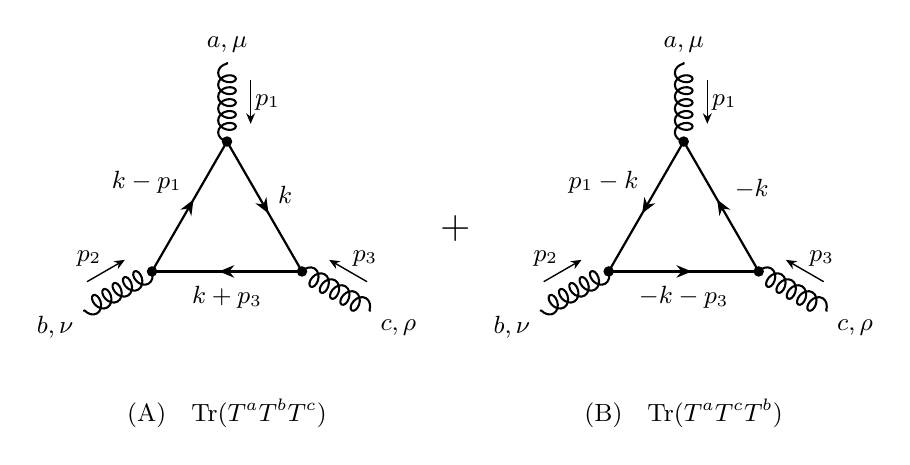
\begin{tikzpicture}[fd]
  \def\fdR{1.1}\def\fdL{1.0}
  % ---------------- diagram A: fermion flows c -> b -> a -> c (clockwise) ----------------
  \begin{scope}
    \coordinate (a) at (90:\fdR); \coordinate (b) at (210:\fdR); \coordinate (c) at (330:\fdR);
    \draw[quark] (c) -- (b); \draw[quark] (b) -- (a); \draw[quark] (a) -- (c);
    \draw[gluon] (a) -- (90:\fdR+\fdL) coordinate (ea);
    \draw[gluon] (b) -- (210:\fdR+\fdL) coordinate (eb);
    \draw[gluon] (c) -- (330:\fdR+\fdL) coordinate (ec);
    \path[mom sep=0.3cm,mom={$p_1$}] (ea) -- (a);
    \path[mom sep=0.3cm,mom={$p_2$}] (eb) -- (b);
    \path[mom sep=0.3cm,mom'={$p_3$}] (ec) -- (c);
    \node[above] at (ea) {$a,\mu$};
    \node[anchor=30] at (eb) {$b,\nu$};
    \node[anchor=150] at (ec) {$c,\rho$};
    \foreach \pp in {a,b,c} \node[vertex] at (\pp) {};
    \node[anchor=210,inner sep=4.5pt] at ($(a)!0.5!(c)$) {$k$};
    \node[anchor=-30,inner sep=4.5pt] at ($(b)!0.5!(a)$) {$k-p_1$};
    \node[below,inner sep=5pt] at ($(c)!0.5!(b)$) {$k+p_3$};
    \node at (0,-2.35) {(A)\quad $\Tr(T^aT^bT^c)$};
  \end{scope}
  \node[font=\Large] at (2.9,0) {$+$};
  % ---------------- diagram B: fermion flows a -> b -> c -> a (counterclockwise) ----------------
  \begin{scope}[xshift=5.8cm]
    \coordinate (a) at (90:\fdR); \coordinate (b) at (210:\fdR); \coordinate (c) at (330:\fdR);
    \draw[quark] (a) -- (b); \draw[quark] (b) -- (c); \draw[quark] (c) -- (a);
    \draw[gluon] (a) -- (90:\fdR+\fdL) coordinate (ea);
    \draw[gluon] (b) -- (210:\fdR+\fdL) coordinate (eb);
    \draw[gluon] (c) -- (330:\fdR+\fdL) coordinate (ec);
    \path[mom sep=0.3cm,mom={$p_1$}] (ea) -- (a);
    \path[mom sep=0.3cm,mom={$p_2$}] (eb) -- (b);
    \path[mom sep=0.3cm,mom'={$p_3$}] (ec) -- (c);
    \node[above] at (ea) {$a,\mu$};
    \node[anchor=30] at (eb) {$b,\nu$};
    \node[anchor=150] at (ec) {$c,\rho$};
    \foreach \pp in {a,b,c} \node[vertex] at (\pp) {};
    \node[anchor=210,inner sep=4.5pt] at ($(a)!0.5!(c)$) {$-k$};
    \node[anchor=-30,inner sep=4.5pt] at ($(b)!0.5!(a)$) {$p_1-k$};
    \node[below,inner sep=5pt] at ($(c)!0.5!(b)$) {$-k-p_3$};
    \node at (0,-2.35) {(B)\quad $\Tr(T^aT^cT^b)$};
  \end{scope}
\end{tikzpicture}
\caption{三胶子函数的单圈夸克三角图。外胶子 $(a,\mu,p_1)$、$(b,\nu,p_2)$、$(c,\rho,p_3)$ 的动量全部流入，$p_1+p_2+p_3=0$。
以顶点所连外胶子的色指标标记顶点，(A) 是循环 $\ell=(a\,b\,c)$，费米子沿 $c\to b\to a\to c$（顺时针）流动；
(B) 是其反向循环 $\bar\ell=(a\,c\,b)$，费米子沿 $a\to b\to c\to a$（逆时针）流动。
内线旁标注的是沿费米子箭头方向的动量（镜像动量配置：同一条内线在两图中携带相同的物理动量），
其中 $k$ 为圈动量（记号同\cref{sec:triangle}，与本节中表示顶点数的 $k$ 无关）；下方为逆着箭头读出的色因子。}
\label{fig:triangles}
\end{figure}

\paragraph{三角图。}三个外胶子直接连在同一个夸克圈上的单圈贡献恰是一对循环 $\ell=(a\,b\,c)$、$\bar\ell=(a\,c\,b)$（\cref{lem:thmI-pairs}，\cref{fig:triangles}）。
(B) 的色因子 $\Tr(T^aT^cT^b)=\Tr(T^cT^bT^a)$ 是反序迹；在镜像动量配置下，由\cref{eq:loop-reversal-mom}，(B) 的 Dirac 迹逐点是 (A) 的 $(-1)^3$ 倍，
故两图之和的色因子为 $\Tr(T^a[T^b,T^c])=\frac{\ii}{2}f^{abc}$：$d^{abc}$ 部分相消、$f^{abc}$ 部分相加（参见\cite{BlumAlkoferHuberWindisch2015}；
两图相加而非相消亦见\cite{DavydychevOslandSaks2001}；“偶数个顶点给出 $\Real\Tr$、奇数个给出 $\ii\Imag\Tr$”见\cite{PastonProkhvatilovFranke1999}）。具体地（Gell-Mann 基，\cref{app:su3}），$(a,b,c)=(1,1,8)$ 时两图的色因子同为
$\frac14d^{118}=\frac{1}{4\sqrt3}$，每个图都不为零，但 Dirac 部分反号，和为零（$f^{118}=0$）；$(a,b,c)=(1,2,3)$ 时 $\Tr(T^1T^2T^3)=\frac{\ii}{4}=-\Tr(T^1T^3T^2)$，两图相加。
\cref{sec:triangle}将显式计算这一对图（\cref{prop:triangle}），并说明仅凭 Bose 对称性不能排除 $d^{abc}$ 乘以全对称运动学张量的结构，排除它的正是 C。

\paragraph{方框图。}设外胶子 $(a_j,\mu_j,p_j)$（流入）依次连在 $\ell=(1\,2\,\cdots\,k)$ 的顶点 $j$ 上，沿箭头由 $z_{j+1}$ 到 $z_j$ 的内线携带 $q_j$：
$q_k=l$（圈动量），$q_{j-1}=q_j+p_j$（由 $\sum_jp_j=0$，顶点 $1$ 处也守恒；即\cref{eq:dirac-polygon}）；$\bar\ell$ 取镜像配置，同一内线沿反向箭头携带 $-q_j$。截腿贡献
\[
\mathcal M_\ell=-(\ii g)^k\,\tau_\ell\int\frac{\dd^Dl}{(2\pi)^D}\TrD\bigl[\gamma^{\mu_1}S(q_1)\cdots\gamma^{\mu_k}S(q_k)\bigr]
\]
（$k=3$ 即\cref{sec:triangle}的 $M_A$）与 $\mathcal M_{\bar\ell}$ 的 Dirac 被积函数逐点相差 $(-1)^k$（\cref{eq:loop-reversal-mom}）。$k=4$ 时六个循环构成三对（\cref{fig:boxes}），每对的 Dirac 部分相等、色因子互为复共轭（\cref{eq:color-reversal}），故
\begin{equation}\label{eq:thmI-box}
\sum_{\text{六个循环}}\mathcal M_\ell=-2g^4\!\!\sum_{\sigma\in\{(1234),(1243),(1324)\}}\!\!\Real\Tr\bigl(T^{a_1}T^{a_{\sigma_2}}T^{a_{\sigma_3}}T^{a_{\sigma_4}}\bigr)\,I_\sigma ,
\end{equation}
其中 $\sigma=(1\,\sigma_2\,\sigma_3\,\sigma_4)$，$I_\sigma$ 是循环 $\sigma$ 的 Dirac 圈积分，而 $\Real\Tr(T^aT^bT^cT^d)=\frac{1}{4N}\delta^{ab}\delta^{cd}+\frac18(d^{abe}d^{cde}-f^{abe}f^{cde})$：
直接连在夸克圈上的四胶子贡献不含 C~奇结构 $d^{abe}f^{cde}$、$f^{abe}d^{cde}$。只要正规化方案对两个被积函数（作为同一 $l$ 的函数）作相同的处理，这一配对就成立；
一般 $k$ 的色序振幅反射恒等式见\cref{prop:app-reflection}。

\begin{figure}[tb]
\centering
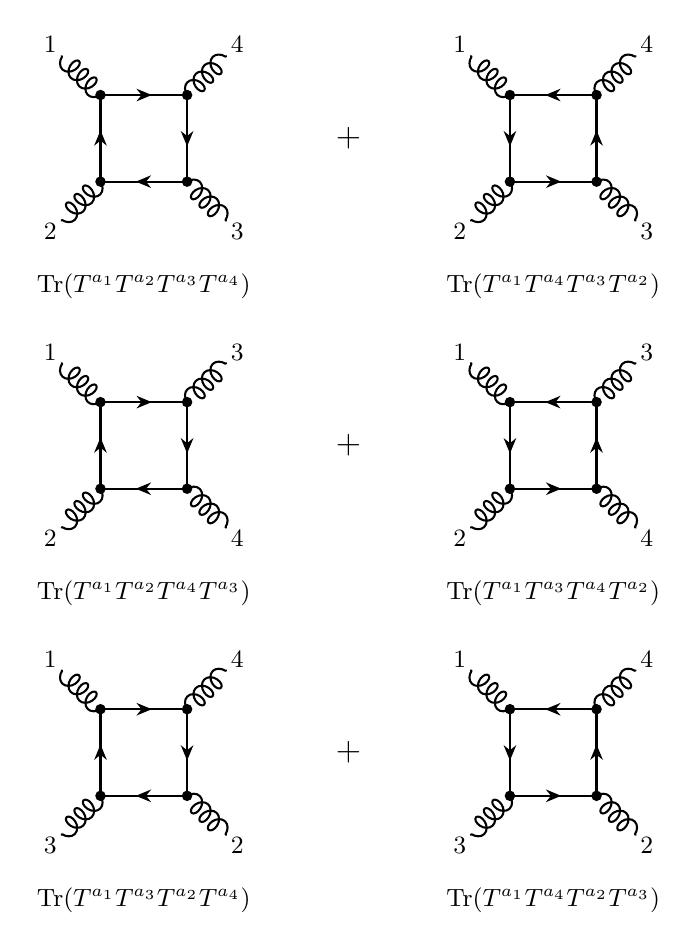
\begin{tikzpicture}[fd]
  \def\fdh{0.55}\def\fdL{0.7}
  % #1,#2: centre; #3..#6: labels at TL, BL, BR, TR; #7: directed edges; #8: colour factor
  \def\fdBox#1#2#3#4#5#6#7#8{%
    \begin{scope}[shift={(#1,#2)}]
      \coordinate (TL) at (-\fdh,\fdh); \coordinate (BL) at (-\fdh,-\fdh);
      \coordinate (BR) at (\fdh,-\fdh); \coordinate (TR) at (\fdh,\fdh);
      \foreach \src/\dst in #7 \draw[quark] (\src) -- (\dst);
      \foreach \pp/\ang/\lab in {TL/135/#3,BL/225/#4,BR/315/#5,TR/45/#6}{
        \draw[gluon] (\pp) -- ++(\ang:\fdL) node[shift={(\ang:0.2)}]{$\lab$};
        \node[vertex] at (\pp) {};}
      \node at (0,-1.88) {#8};
    \end{scope}}
  \def\cw{TL/TR,TR/BR,BR/BL,BL/TL}
  \def\ccw{TL/BL,BL/BR,BR/TR,TR/TL}
  % row 1: (1234) and (1432)
  \fdBox{0}{0}{1}{2}{3}{4}{\cw}{$\Tr(T^{a_1}T^{a_2}T^{a_3}T^{a_4})$}
  \node[font=\large] at (2.6,0) {$+$};
  \fdBox{5.2}{0}{1}{2}{3}{4}{\ccw}{$\Tr(T^{a_1}T^{a_4}T^{a_3}T^{a_2})$}
  % row 2: (1243) and (1342)
  \fdBox{0}{-3.9}{1}{2}{4}{3}{\cw}{$\Tr(T^{a_1}T^{a_2}T^{a_4}T^{a_3})$}
  \node[font=\large] at (2.6,-3.9) {$+$};
  \fdBox{5.2}{-3.9}{1}{2}{4}{3}{\ccw}{$\Tr(T^{a_1}T^{a_3}T^{a_4}T^{a_2})$}
  % row 3: (1324) and (1423)
  \fdBox{0}{-7.8}{1}{3}{2}{4}{\cw}{$\Tr(T^{a_1}T^{a_3}T^{a_2}T^{a_4})$}
  \node[font=\large] at (2.6,-7.8) {$+$};
  \fdBox{5.2}{-7.8}{1}{3}{2}{4}{\ccw}{$\Tr(T^{a_1}T^{a_4}T^{a_2}T^{a_3})$}
\end{tikzpicture}
\caption{四胶子函数的六个单圈夸克方框图（四个外胶子的 $3!=6$ 种循环次序，数字 $j$ 代表外胶子 $(a_j,\mu_j)$）。每一行是一对互为反射（取向相反）的图；
图下为逆着费米子箭头读出的色因子，同一行两图的色因子互为复共轭，故每行两图之和的色因子为 $2\Real\Tr(\cdots)$（\cref{eq:thmI-box}）。}
\label{fig:boxes}
\end{figure}

%% ----------------------------------------------------------------------
\subsection{色单态插入}\label{sec:thmI-singlet}

夸克圈上还可以有色单态顶点：电磁流、$Z$ 玻色子流的矢量与轴矢部分、Higgs 的 Yukawa 耦合，或作为外源插入的复合算符 $\bar\psi\Gamma\psi$。

\begin{corollary}[色单态插入]\label{cor:singlet}
设圈上有 $k_g$ 个夸克--胶子顶点（沿逆箭头方向色指标依次为 $a_1,\dots,a_{k_g}$）与 $m$ 个味对角的色单态顶点
$\kappa_j'\,\Gamma_j'\otimes\mathbb 1$（C~宇称为 $\eta_j'$），$k_g+m\ge3$，并令 $\eta=\prod_{j=1}^m\eta_j'$。则
\begin{equation}\label{eq:furry-singlet}
L_\ell+L_{\bar\ell}=-(\ii g)^{k_g}\Bigl(\prod_{j=1}^m\kappa'_j\Bigr)K_\ell\Bigl[\tau+(-1)^{k_g}\eta\,\tau^{\mathrm{rev}}\Bigr]
=-(\ii g)^{k_g}\Bigl(\prod_{j=1}^m\kappa'_j\Bigr)K_\ell\cdot2\,(\mathcal P_\eta\tau),
\end{equation}
其中 $\tau=\Tr(T^{a_1}\cdots T^{a_{k_g}})$，$\tau^{\mathrm{rev}}=\Tr(T^{a_{k_g}}\cdots T^{a_1})$；$k_g=0$ 时 $\tau=\tau^{\mathrm{rev}}=N$。
\end{corollary}

\begin{proof}
把\cref{thm:furry-single}应用于全部 $k_g+m$ 个顶点（按沿圈的实际次序，可任意交错），$K_\ell$ 是含全部 $\Gamma_j'$ 的 Dirac 因子，耦合常数之积为 $(\ii g)^{k_g}\prod_j\kappa_j'$。
单态顶点的 $M=\mathbb 1$、$M^{\mathsf c}=\eta_j'\mathbb 1$ 在迹中只贡献纯数，故 $\Tr(M_1\cdots M_k)=\tau$；由\cref{lem:thmI-transpose}，
$\Tr(M_1^{\mathsf c}\cdots M_k^{\mathsf c})=\eta(-1)^{k_g}\Tr\bigl((T^{a_1})^{\tp}\cdots(T^{a_{k_g}})^{\tp}\bigr)=\eta(-1)^{k_g}\tau^{\mathrm{rev}}$。代入\cref{eq:furry-master}即得第一个等式。
对 $k_g\ge1$，由\cref{eq:color-reversal}，$(-1)^{k_g}\tau^{\mathrm{rev}}=\Rop\tau$，方括号等于 $(1+\eta\Rop)\tau=2\mathcal P_\eta\tau$；对 $k_g=0$，$\Rop$ 作用于数是恒等映射，方括号为 $N(1+\eta)$。
\end{proof}

$k_g+m\le2$ 时 $\bar\ell=\ell$，$L_\ell$ 是\cref{eq:furry-singlet}右端的一半。多个味道时，由于各顶点都是味对角的，每个闭合圈只含一个味道；
味对角算符 $\sum_f\kappa_j^{(f)}\bar\psi_f\Gamma_j'\psi_f$ 在味道为 $f$ 的圈上给出 $\kappa_j'=\kappa_j^{(f)}$，推论对每个味道分别成立（味非对角的情形见\cref{rem:thmI-flavour}）。与\cref{eq:thmI-C-image}同样地，
\begin{equation}\label{eq:thmI-C-image-singlet}
L_{\bar\ell}=\eta\,\Rop L_\ell ,\qquad \Rop\bigl(L_\ell+L_{\bar\ell}\bigr)=\eta\,\bigl(L_\ell+L_{\bar\ell}\bigr)
\end{equation}
（后者用了 $\Rop^2=1$）：\emph{一对取向之和在外胶子色指标上的 \textup{C}~宇称，等于圈上全部色单态插入的 \textup{C}~宇称之积}，这是选择定则（\cref{eq:selection-rule}）的单圈“种子”。
在\cref{fig:mixed}(a)（$\gamma^*gg$，$\eta=-1$）中两图的色因子同为 $\frac12\delta^{ab}$，Dirac 部分因三个矢量顶点而反号，和为零；
在\cref{fig:mixed}(b)（$\gamma^*ggg$）中，\cref{eq:furry-singlet}的方括号为 $\tau+\tau^{\mathrm{rev}}=2\Pm\tau=\frac12d^{abc}$，与纯胶子情形相反，$f^{abc}$ 部分相消，故 $\mathrm{SU}(2)$ 中为零；单圈 $\gamma^*ggg$ 的 $3!=6$ 个方框图构成三对，
每对的方括号都是 $\frac12d^{abc}$。

\begin{figure}[htbp]
\centering
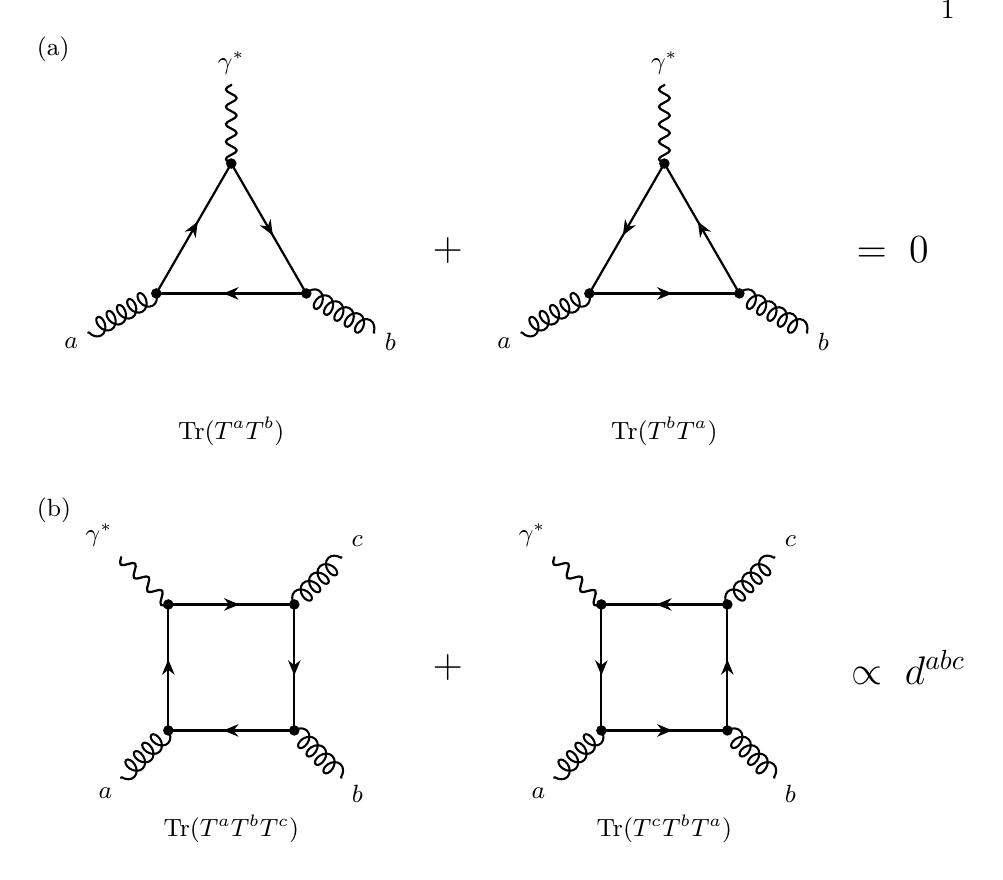
\begin{tikzpicture}[fd]
  \def\fdR{1.1}\def\fdL{1.0}
  \node[anchor=west] at (-2.6,2.55) {(a)};
  \begin{scope}
    \coordinate (a) at (90:\fdR); \coordinate (b) at (210:\fdR); \coordinate (c) at (330:\fdR);
    \draw[quark] (c) -- (b); \draw[quark] (b) -- (a); \draw[quark] (a) -- (c);
    \draw[photon] (a) -- (90:\fdR+\fdL) node[above]{$\gamma^*$};
    \draw[gluon] (b) -- (210:\fdR+\fdL) node[anchor=30]{$a$};
    \draw[gluon] (c) -- (330:\fdR+\fdL) node[anchor=150]{$b$};
    \foreach \pp in {a,b,c} \node[vertex] at (\pp) {};
    \node at (0,-2.3) {$\Tr(T^aT^b)$};
  \end{scope}
  \node[font=\Large] at (2.75,0) {$+$};
  \begin{scope}[xshift=5.5cm]
    \coordinate (a) at (90:\fdR); \coordinate (b) at (210:\fdR); \coordinate (c) at (330:\fdR);
    \draw[quark] (a) -- (b); \draw[quark] (b) -- (c); \draw[quark] (c) -- (a);
    \draw[photon] (a) -- (90:\fdR+\fdL) node[above]{$\gamma^*$};
    \draw[gluon] (b) -- (210:\fdR+\fdL) node[anchor=30]{$a$};
    \draw[gluon] (c) -- (330:\fdR+\fdL) node[anchor=150]{$b$};
    \foreach \pp in {a,b,c} \node[vertex] at (\pp) {};
    \node at (0,-2.3) {$\Tr(T^bT^a)$};
  \end{scope}
  \node[font=\Large] at (8.4,0) {$=\;0$};
  % ---------------- (b) photon + three gluons ----------------
  \def\fdh{0.8}\def\fdLb{0.85}
  \node[anchor=west] at (-2.6,-3.3) {(b)};
  \begin{scope}[yshift=-5.3cm]
    \coordinate (TL) at (-\fdh,\fdh); \coordinate (BL) at (-\fdh,-\fdh);
    \coordinate (BR) at (\fdh,-\fdh); \coordinate (TR) at (\fdh,\fdh);
    \foreach \src/\dst in {TL/TR,TR/BR,BR/BL,BL/TL} \draw[quark] (\src) -- (\dst);
    \draw[photon] (TL) -- ++(135:\fdLb) node[anchor=-45]{$\gamma^*$};
    \draw[gluon] (BL) -- ++(225:\fdLb) node[anchor=45]{$a$};
    \draw[gluon] (BR) -- ++(315:\fdLb) node[anchor=135]{$b$};
    \draw[gluon] (TR) -- ++(45:\fdLb) node[anchor=-135]{$c$};
    \foreach \pp in {TL,BL,BR,TR} \node[vertex] at (\pp) {};
    \node at (0,-2.05) {$\Tr(T^aT^bT^c)$};
  \end{scope}
  \node[font=\Large] at (2.75,-5.3) {$+$};
  \begin{scope}[xshift=5.5cm,yshift=-5.3cm]
    \coordinate (TL) at (-\fdh,\fdh); \coordinate (BL) at (-\fdh,-\fdh);
    \coordinate (BR) at (\fdh,-\fdh); \coordinate (TR) at (\fdh,\fdh);
    \foreach \src/\dst in {TL/BL,BL/BR,BR/TR,TR/TL} \draw[quark] (\src) -- (\dst);
    \draw[photon] (TL) -- ++(135:\fdLb) node[anchor=-45]{$\gamma^*$};
    \draw[gluon] (BL) -- ++(225:\fdLb) node[anchor=45]{$a$};
    \draw[gluon] (BR) -- ++(315:\fdLb) node[anchor=135]{$b$};
    \draw[gluon] (TR) -- ++(45:\fdLb) node[anchor=-135]{$c$};
    \foreach \pp in {TL,BL,BR,TR} \node[vertex] at (\pp) {};
    \node at (0,-2.05) {$\Tr(T^cT^bT^a)$};
  \end{scope}
  \node[font=\Large,anchor=west] at (7.75,-5.3) {$\propto\; d^{abc}$};
\end{tikzpicture}
\caption{含一个色单态光子顶点（C~宇称 $\eta=-1$）的夸克圈（\cref{cor:singlet}）。(a) $\gamma^*gg$：两图色因子同为 $\tfrac12\delta^{ab}$，
Dirac 部分反号，和为零；(b) $\gamma^*ggg$：两种取向之和的色结构为 $\tfrac12d^{abc}$，$f^{abc}$ 部分相消。}
\label{fig:mixed}
\end{figure}

\begin{table}[tb]
\centering
\caption{按机制对若干过程分类。$(k_g,\eta)$ 的记号同\cref{cor:singlet}（无插入时 $\eta=1$）；“色括号”是\cref{eq:furry-singlet}中最低阶两种取向之和的色因子 $\tau+(-1)^{k_g}\eta\,\tau^{\mathrm{rev}}$（无色单态插入时即\cref{eq:bracket}中的 Furry 组合~$B$）；
末列为推广到任意阶所需的条件（“Schur”与“分类”指\cref{lem:invariants}中 $\mathrm{Inv}_2$ 与 $\mathrm{Inv}_3$ 的结构，需要整体 $\mathrm{SU}(N)$ 不变性，见\cref{cor:selection}）。
夸克偶素各行把色单态投影视为 C~宇称为 $(-1)^{L+S}$ 的插入（S~波最低阶见\cref{prop:app-quarkonium}；$L\neq0$ 与任意阶只给出论证要点，见\cref{rem:app-onium-allorders}）。}
\label{tab:thmI-examples}
\small
\renewcommand{\arraystretch}{1.1}
\begin{tabularx}{\textwidth}{@{}l c l l >{\raggedright\arraybackslash}X@{}}
\toprule
过程 & $(k_g,\eta)$ & 色括号（最低阶） & 结论 & 机制（任意阶所需条件） \\
\midrule
$\gamma^*g$ & $(1,-1)$ & 自反向圈；$\Tr T^a=0$ & $0$ & 色不变性（$\mathrm{Inv}_1=0$）；不需要 C \\
$\gamma\gamma g$ & $(1,+1)$ & $0$；每一取向已 $\propto\Tr T^a=0$ & $0$ & 色不变性（$\mathrm{Inv}_1=0$）；不需要 C \\
$\gamma^*gg$ & $(2,-1)$ & $\Tr(T^aT^b)-\Tr(T^bT^a)=0$ & $0$ & C~与 Schur 同时需要 \\
$\gamma\gamma gg$ & $(2,+1)$ & $\delta^{ab}$ & $\propto\delta^{ab}$ & C~允许；Schur 给出 $\propto\delta^{ab}$ \\
$Hgg$，$J_5^\mu gg$ & $(2,+1)$ & $\delta^{ab}$ & $\propto\delta^{ab}$ & C~允许；Schur 给出 $\propto\delta^{ab}$ \\
$ggg$ & $(3,+1)$ & $\frac{\ii}{2}f^{abc}$ & $\propto f^{abc}$ & C $+$ 分类（无分类时：$d^{abc}G^{abc}=0$） \\
$\gamma^*ggg$ & $(3,-1)$ & $\frac12d^{abc}$ & $\propto d^{abc}$ & C $+$ 分类；$\mathrm{SU}(2)$ 中为零 \\
$J_5^\mu ggg$ & $(3,+1)$ & $\frac{\ii}{2}f^{abc}$ & $\propto f^{abc}$ & C $+$ 分类 \\
$\gamma\gamma\gamma$ & $(0,-1)$ & $N(1-1)=0$ & $0$ & C（\cref{cor:selection}(c)） \\
\midrule
$J/\psi\to gg$ & $(2,-1)$ & $0$ & $0$ & C~与 Schur 同时需要；在壳时亦被 Landau--Yang 禁戒 \\
$\eta_c\to gg$ & $(2,+1)$ & $\delta^{ab}$ & 允许 & C~允许；Schur 给出 $\propto\delta^{ab}$ \\
$\chi_{c1}\to gg$ & $(2,+1)$ & $\delta^{ab}$ & 在壳为零 & C~允许；Landau--Yang 禁戒 \\
$J/\psi\to ggg$ & $(3,-1)$ & $\frac12d^{abc}$ & $\propto d^{abc}$ & C $+$ 分类；$\mathrm{SU}(2)$ 中为零 \\
\bottomrule
\end{tabularx}
\end{table}

\paragraph{按机制分类。}\cref{tab:thmI-examples}把常被统称为“Furry 定理的推论”的结论按真正的来源分类。(1) $\gamma\gamma g=0$ \emph{不是} C~的结果：
每个取向单独已正比于 $\Tr T^a=0$；在任意阶，$G^a$ 是不变的单指标张量而 $\mathrm{Inv}_1=0$，C~只说明它是 C~偶的，并不迫使它为零（$\gamma^*g$ 同理：那里 C~只要求 $G^a$ 为 C~奇，使它为零的仍是 $\mathrm{Inv}_1=0$）。
(2) $\gamma\gamma gg\propto\delta^{ab}$ 也不是 C~的结果：$\eta=+1$ 而 $\delta^{ab}$ 是 C~偶的，C~不施加约束，$\propto\delta^{ab}$ 来自 Schur 引理。
(3) $\gamma^*gg=0$ 在单圈层次上是 C~的直接结果，但在任意阶需要\emph{同时}使用 C~与 Schur 引理：C~要求 $G^{ab}$ 为 C~奇，而 $G^{ab}\propto\delta^{ab}$ 是 C~偶的（\cref{cor:selection}(b)）。
夸克偶素中（任意阶的论证要点见\cref{rem:app-onium-allorders}），$J/\psi$ 衰变为三个胶子\cite{AppelquistPolitzer1975PRL}，其色结构只含 $d^{abc}$~\cite{Ewerz2003,Jia2007}；
$\chi_{c1}\to gg$ 为 C~所允许，在壳时则被 Landau--Yang 定理\cite{Landau1948,Yang1950}禁戒：该定理断言自旋 $1$ 的粒子不能衰变为两个光子，
它对色对称、$\propto\delta^{ab}$ 的双胶子态同样适用（\cref{rem:app-onium-LY}）。

%% ----------------------------------------------------------------------
\subsection{QED 中的 Furry 定理}\label{sec:thmI-qed}

\cref{thm:furry-single}包含 Furry 的原始定理\cite{Furry1937}（亦见\cite[第~10.1~节]{PeskinSchroeder1995}）。“QED 极限”常被说成“令 $T^a\to1$”，
但这不是有意义的数学操作：$\mathrm{SU}(N)$ 的生成元无迹，$\mathbb 1\notin\su(N)$。它有两种精确含义，即下面的 (i) 与 (ii)。

\begin{corollary}[QED 中的 Furry 定理]\label{cor:qed}
(i) 对 $\mathrm U(1)$ 规范理论（顶点 $-\ii eQ\gamma^\mu$，即 $\kappa=-\ii e$，$\Gamma=\gamma^\mu$，$M=Q$ 为实数，$\eta=-1$），
$L_\ell+L_{\bar\ell}=-(-\ii eQ)^kK_\ell\bigl[1+(-1)^k\bigr]$（$k\le2$ 时 $\bar\ell=\ell$，左端读作 $2L_\ell$）；
因此含奇数个光子顶点的费米子圈为零（$k\ge3$ 时指两种取向之和，$k=1$ 时指 $L_\ell$ 本身），这正是 Furry 的原始定理。
(ii) 在 QCD$+$QED 中，只含光子顶点（$k_g=0$）的夸克圈给出上式的 $N$ 倍。
\end{corollary}

\begin{proof}
(i) $\mathrm U(1)$ 理论的内部空间是一维的。由 $\eta_j=-1$ 得 $M_j^{\mathsf c}=\eta_jM_j^{\tp}=-Q$，故\cref{eq:furry-master}的右端为
$-(-\ii e)^kK_\ell[Q^k+(-Q)^k]=-(-\ii eQ)^kK_\ell[1+(-1)^k]$（把 $Q$ 放进 $\kappa_j$ 结果相同）。由\cref{thm:furry-single}，$k\ge3$ 时它等于 $L_\ell+L_{\bar\ell}$，
左端是两个不同项之和，$k$ 为奇数时为零；$k\le2$ 时 $\bar\ell=\ell$，$L_\ell$ 是它的一半，即左端读作 $2L_\ell$：$k=1$ 给出 $L_\ell=0$，
$k=2$ 给出真空极化 $L_\ell=e^2Q^2K_\ell$，一般不为零。
(ii) 光子与 $f$ 味夸克的顶点 $-\ii eQ_f\gamma^\mu\otimes\mathbb 1$ 是味对角的色单态顶点（$\eta_j'=-1$）。$k\ge3$ 时在\cref{cor:singlet}中取 $k_g=0$，$m=k$，$\kappa_j'=-\ii eQ_f$，
$\eta=(-1)^k$，$\tau=\tau^{\mathrm{rev}}=N$，即得 $-(-\ii eQ_f)^kK_\ell\,N[1+(-1)^k]$。$k\le2$ 时\cref{cor:singlet}的条件 $k_g+m\ge3$ 不成立，
改在\cref{thm:furry-single}中取 $\kappa_j=-\ii eQ_f$，$\Gamma_j=\gamma^{\mu_j}$，$M_j=\mathbb 1$（$M_j^{\mathsf c}=-\mathbb 1$），得 $L_\ell$ 等于同一式的一半，即左端同样读作 $2L_\ell$。
\end{proof}

\begin{figure}[htbp]
\centering
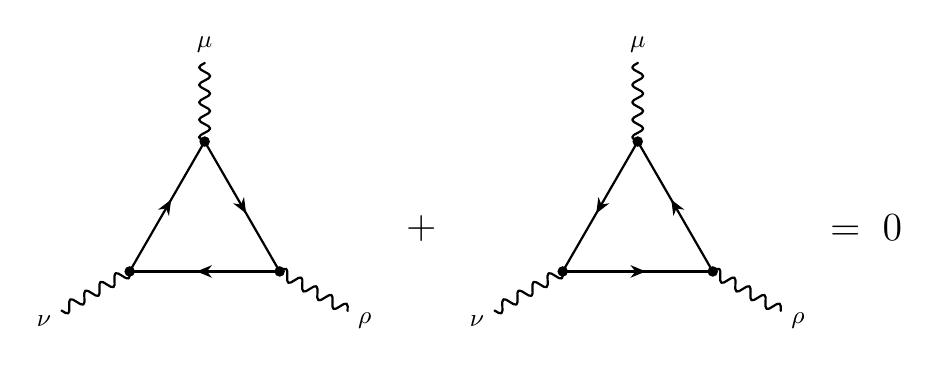
\begin{tikzpicture}[fd]
  \def\fdR{1.1}\def\fdL{1.0}
  \begin{scope}
    \coordinate (a) at (90:\fdR); \coordinate (b) at (210:\fdR); \coordinate (c) at (330:\fdR);
    \draw[quark] (c) -- (b); \draw[quark] (b) -- (a); \draw[quark] (a) -- (c);
    \draw[photon] (a) -- (90:\fdR+\fdL) node[above]{$\mu$};
    \draw[photon] (b) -- (210:\fdR+\fdL) node[anchor=30]{$\nu$};
    \draw[photon] (c) -- (330:\fdR+\fdL) node[anchor=150]{$\rho$};
    \foreach \pp in {a,b,c} \node[vertex] at (\pp) {};
  \end{scope}
  \node[font=\Large] at (2.75,0) {$+$};
  \begin{scope}[xshift=5.5cm]
    \coordinate (a) at (90:\fdR); \coordinate (b) at (210:\fdR); \coordinate (c) at (330:\fdR);
    \draw[quark] (a) -- (b); \draw[quark] (b) -- (c); \draw[quark] (c) -- (a);
    \draw[photon] (a) -- (90:\fdR+\fdL) node[above]{$\mu$};
    \draw[photon] (b) -- (210:\fdR+\fdL) node[anchor=30]{$\nu$};
    \draw[photon] (c) -- (330:\fdR+\fdL) node[anchor=150]{$\rho$};
    \foreach \pp in {a,b,c} \node[vertex] at (\pp) {};
  \end{scope}
  \node[font=\Large] at (8.4,0) {$=\;0$};
\end{tikzpicture}
\caption{QED 中的 Furry 定理（\cref{cor:qed}）：三光子顶点的两个三角图（费米子圈取向相反）互相抵消。
把\cref{fig:triangles}中的胶子换成光子即得；两图的耦合因子相同，均为 $(-\ii eQ)^3$，而 Dirac 部分只差因子 $(-1)^3$。}
\label{fig:qed-triangles}
\end{figure}

在含义 (i) 中，$\varphi(X)=-X^{\tp}$ 作用于 $1\times1$ 矩阵就是 $X\mapsto-X$，C~作用于含 $n$ 个光子的函数就是乘以 $(-1)^n$（\cref{fig:qed-triangles}；对 $k=4$ 的光--光散射，方括号 $1+(-1)^k$ 等于 $2$，
两种取向相加）。在含义 (ii) 中，光子是夸克圈上的色单态插入，图的其余部分可含任意多的胶子；\cref{cor:selection}(c) 把它推广到 $\alpha_s$ 的任意阶。

%% ----------------------------------------------------------------------
\subsection{若干注记}\label{sec:thmI-remarks}

\begin{remark}[长度 $k\le2$ 的圈]\label{rem:thmI-short-loops}
$k\le2$ 时 $\bar\ell=\ell$，\cref{eq:closed-loops}中只有一项，把\cref{eq:furry-master}的左端读作两个缩并之和会重复计数。此时：(1) $L_\ell$ 是\cref{eq:furry-master}右端的一半，
对夸克--胶子顶点即 $L_\ell=-(\ii g)^kK_\ell\tau$，$\tau^a=0$ 与 $\tau^{ab}=\frac12\delta^{ab}$ 本身是 C~偶的——夸克圈对胶子自能的贡献是\emph{一个}缩并而不是一对；
(2) 由于 $K_{\bar\ell}=K_\ell$，证明第二步的\cref{eq:thmI-dirac-step}成为一致性条件 $K_\ell=(\prod_j\eta_j)K_\ell$；
因 $k\le2$ 时 $\Tr(M_1^{\mathsf c}\cdots M_k^{\mathsf c})=(\prod_j\eta_j)\Tr(M_1\cdots M_k)$，\cref{eq:master}只是这一条件两端乘以 $-(\prod_j\kappa_j)\Tr(M_1\cdots M_k)$ 所得，
在这个色迹为零时不含信息。由一致性条件，$\prod_j\eta_j=-1$ 时 $K_\ell=0$，例如矢量“蝌蚪图” $\TrD[\gamma^\mu S_{\mathrm{reg}}(0)]=0$，
以及矢量流与标量密度混合的两点函数 $\TrD[\gamma^\mu\SF(x)\SF(-x)]=0$。这一条件在坐标空间中由 (R1) 逐点成立（正规化传播子须在顶点重合处也有定义）；
在动量空间中它不是逐点的，而要求正规化后的圈积分在镜像重参数化下不变，即 (R2) 对自反向圈的要求——维数正规化满足之，朴素截断则不一定
（直接验证与重参数化的具体形式见\cref{sec:dirac-loop}的“短圈”一段，详见\cref{rem:reg-selfreverse}）。\cref{sec:thmII}的整体对合
$\rho$ 把这样的循环映为自身，无需与另一缩并配对，所需的只是这一一致性条件（在动量空间中即上述积分条件，见\cref{lem:thmII-rho-value}的第四步）。
\end{remark}

\begin{remark}[任意表示与 $N=2$]\label{rem:thmI-rep}
若夸克处于任一有限维酉表示 $r$，则 $M^{\mathsf c}=-(T^a_r)^{\tp}=T^a_{\bar r}$，由\cref{thm:furry-single}与\cref{lem:color-reversal}，$k\ge3$ 时两种取向之和正比于
$\tau_r+\tau_{\bar r}=2\Pp\tau_r$。(1) 若 $r\simeq\bar r$（实或赝实表示，如伴随表示及 $\mathrm{SU}(2)$ 的一切表示），则 $T^a_{\bar r}=UT^a_rU^{-1}$，$\tau_{\bar r}=\tau_r$，
$L_{\bar\ell}=L_\ell$：两种取向相等，定理对色结构不施加约束（$\mathrm{SU}(2)$ 见\cref{prop:su2}）。(2) 只有复表示才有非零的 C~奇部分；$k=3$、$N\ge3$ 时
它是 $\frac14A(r)d^{abc}$，相消即 $A(r)+A(\bar r)=0$（$A(r)$ 的定义及其与反常相消的关系见\cref{rem:color-anomaly}）。
(3) 手征耦合须先按\cref{rem:thmI-decomposition}分解；手征规范理论中 C~不是对称性。对建立在单紧 Lie 代数某一不可约表示上、且无 $\gamma^5$ 反常的
非 Abel 规范拉氏量，总可以定义使拉氏量不变的 C~宇称\cite{Smolyakov1982}。
\end{remark}

\begin{remark}[味结构]\label{rem:thmI-flavour}
对味非对角顶点 $\kappa\,\Gamma\otimes M\otimes\Lambda$（$\Lambda$ 为味矩阵），把味指标并入内部指标，Dirac~$\otimes$~味空间上的传播子为 $\mathbf S_F(x)=\sum_f\SF^{(f)}(x)\otimes E_{ff}$（$E_{ff}$ 为到第 $f$ 味的投影，各味质量可不同），\cref{lem:closed-loops}的证明对这样的内部空间同样成立。记 $K_\ell[\Lambda_1,\dots,\Lambda_k]$ 为把\cref{eq:thmI-L}中的
$\Gamma_j$、$\SF$ 换成 $\Gamma_j\otimes\Lambda_j$、$\mathbf S_F$ 并对 Dirac~$\otimes$~味求迹所得的因子。用 $X\mapsto(C\otimes\mathbb 1)X^{\tp}(C\otimes\mathbb 1)^{-1}$（Dirac 与味同时转置，
仍是保迹的反自同构；$E_{ff}^{\tp}=E_{ff}$ 保证 $\mathbf S_F(x)\mapsto\mathbf S_F(-x)$）代替\cref{eq:thmI-dirac-step}中的 $X\mapsto\Cconj X$，同一论证给出
\begin{equation}\label{eq:thmI-flavour}
K_{\bar\ell}[\Lambda_1,\dots,\Lambda_k]=\Bigl(\prod_{j=1}^k\eta_j\Bigr)K_\ell[\Lambda_1^{\tp},\dots,\Lambda_k^{\tp}] ,
\end{equation}
即 $M^{\mathsf c}=\eta M^{\tp}$ 中的转置应对色与味\emph{同时}进行。若全部 $\Lambda_j$ 对称（特别地，味对角），前述结论不变；否则\cref{eq:thmI-flavour}联系的是\emph{两个不同过程}：
例如带电流的矢量部分 $\bar u\gamma^\mu d$（$W^+$ 顶点，$\Lambda=E_{ud}$）在反向圈中变为 $\bar d\gamma^\mu u$（$W^-$ 顶点），Furry 配对给出含 $W^+$ 与含 $W^-$ 的过程之间的关系，
而不使任何一个为零（完整的带电流耦合是手征的，须先按\cref{rem:thmI-decomposition}分解）。
\end{remark}

\begin{remark}[含导数的耦合]\label{rem:thmI-derivative}
若顶点含作用于夸克场的导数（如能量--动量张量 $\bar\psi\gamma^\mu\ii\overleftrightarrow{\partial^\nu}\psi$），把它写成动量空间的顶点函数 $V(p_{\mathrm{in}},p_{\mathrm{out}})$，
$p_{\mathrm{in}}$（$p_{\mathrm{out}}$）为沿费米子箭头流入（流出）的夸克动量（此时\cref{lem:closed-loops}的推广\cref{prop:app-wick-cycles}仍给出同样形式的圈因子，
只是顶点矩阵依赖于动量）；“$\Gamma$ 的 C~宇称为 $\eta$”应代之以
\begin{equation}\label{eq:thmI-derivative}
\Cconj{V(p_{\mathrm{in}},p_{\mathrm{out}})}=\eta\,V(-p_{\mathrm{out}},-p_{\mathrm{in}}) .
\end{equation}
理由：镜像动量配置下，顶点在 $\bar\ell$ 中的流入线是它在 $\ell$ 中的流出线，且沿新箭头的动量反号，故 $\bar\ell$ 中的顶点函数是 $V(-p_{\mathrm{out}},-p_{\mathrm{in}})$；
再像\cref{eq:thmI-dirac-step}那样利用\cref{eq:thmI-derivative}与 $\Cconj{S(q)}=S(-q)$，即得 $K_{\bar\ell}=(\prod_j\eta_j)K_\ell$。在场的层次上这对应于
$\bar\psi\,\Gamma\,(\partial_\nu\psi)\mapsto(\partial_\nu\bar\psi)\,\Cconj\Gamma\,\psi$。例如，Gordon 分解中的对流项顶点 $(p_{\mathrm{in}}+p_{\mathrm{out}})^\mu\mathbb 1$ 与磁矩项顶点
$\ii\sigma^{\mu\nu}(p_{\mathrm{out}}-p_{\mathrm{in}})_\nu$ 都有 $\eta=-1$（与 $\gamma^\mu$ 本身的 $\eta=-1$ 一致），而 $\gamma^\mu(p_{\mathrm{in}}+p_{\mathrm{out}})^\nu$ 有 $\eta=+1$：
夸克的能量--动量张量是 C~偶的。
\end{remark}

\begin{remark}[开放夸克线]\label{rem:thmI-open-lines}
对从外点 $y$ 到 $x$ 的开放夸克线
\[
O(x\leftarrow y)=\SF(x-z_1)V_1\SF(z_1-z_2)\cdots V_k\SF(z_k-y)\qquad(V_j=\ii g\gamma^{\mu_j}\otimes T^{a_j}),
\]
同样的论证给出
$(C\otimes\mathbb 1)O(x\leftarrow y)^{\tp}(C\otimes\mathbb 1)^{-1}=\Rop[\SF(y-z_k)V_k\cdots V_1\SF(z_1-x)]$（Dirac 与色部分的两个 $(-1)^k$ 互相抵消）。
右端是沿相反方向传播的另一条线，属于另一个 Green 函数（$\psi$ 与 $\bar\psi$ 互换）：对外夸克，C~只给出夸克与反夸克 Green 函数之间的\emph{关系}，而非选择定则；
例外是把 $q\bar q$ 对投影到确定 C~宇称的色单态（夸克偶素），此时投影起色单态插入的作用（\cref{tab:thmI-examples}，\cref{rem:app-onium-allorders}）。
\end{remark}

%% ======================================================================
%% 第 6 节  显式例子：单圈三胶子顶点
%% ======================================================================
\section{显式例子：单圈三胶子顶点中的夸克圈}\label{sec:triangle}

本节在动量空间中对三个外胶子、一个夸克圈的单圈图完整地验证\cref{thm:furry-single}与\cref{cor:three-four}（长度为 $3$ 的圈）。
它表明三点：(1) 在“镜像动量配置”下，圈反向恒等式是被积函数的逐点恒等式；
(2) Furry 定理并\emph{不}使含奇数个胶子的夸克圈为零，只有色迹的 C~奇部分 $\frac14d^{abc}$ 相消，C~偶部分 $\frac{\ii}{4}f^{abc}$ 加倍，并给出三胶子顶点重整化中的夸克贡献；
(3) 用形式体系中的全部符号与因子（闭合圈的 $-1$、顶点的 $\ii g$、传播子中的 $\ii$、$\Cconj{\gamma^\mu}=-\gamma^\mu$ 带来的 $(-1)^3$ 以及 $T_F=\frac12$）算得的结果，
与 Slavnov--Taylor 恒等式及 $\beta$ 函数中已知的夸克贡献完全一致（参见\cite{DavydychevOslandSaks2001,PeskinSchroeder1995}）。
这里只讨论正比于 $n_f$ 的部分；胶子圈与鬼场圈的色因子是伴随表示的迹，每个取向本身就是 C~偶的（\cref{lem:contraction}）。

\subsection{运动学、带标号的缩并与镜像动量配置}\label{sec:triangle-setup}

\paragraph{约定。}
采用 $D=4-2\epsilon$ 维的维数正规化\cite{tHooftVeltman1972,BolliniGiambiagi1972}：$\TrD$ 如\cref{def:dimreg-trace}（$\TrD\mathbb 1=4$，$g^\mu{}_\mu=D$，不出现 $\gamma^5$）；
圈积分 $\int\frac{\dd^Dk}{(2\pi)^D}$ 是线性的、Lorentz 协变的，并在平移 $k\to k+a$ 与反射 $k\to-k$ 下不变（\cref{prop:reg-dimreg}），凡用到之处均明确指出。
单圈主积分（Minkowski 度规，分母带 $+\ii0$）为
\begin{equation}\label{eq:tri-masters}
\int\frac{\dd^Dk}{(2\pi)^D}\,\frac{(k^2)^n}{(k^2-\Delta)^{r}}=\frac{\ii\,(-1)^{n+r}}{(4\pi)^{D/2}}\,\frac{\Gamma(n+\frac D2)\,\Gamma(r-n-\frac D2)}{\Gamma(\frac D2)\,\Gamma(r)}\,\Delta^{\,n+\frac D2-r}.
\end{equation}
\cref{eq:tri-masters}在 $\Delta>0$ 时由 Wick 转动、$D$ 维球坐标与 Euler Beta 积分直接得到；对一般的实 $\Delta$，把 $\Delta$ 理解为 $\Delta-\ii0$，由向 $\Imag\Delta<0$ 的解析延拓得到，右端的幂取主支。

$S(p)=\ii(\sla p+m)/(p^2-m^2+\ii0)$，$m\ge0$。一切结论对每个味道分别成立，$n_f$ 个味道的贡献相加（质量可各不相同）。
耦合常数 $g\mu^{\epsilon}$ 中的 $\mu^\epsilon$ 不影响任何 $1/\epsilon$ 极点的系数，故不写出；夸克三角图没有胶子内线，因而与规范参数 $\xi$ 无关。

外胶子 $(a,\mu,p_1)$、$(b,\nu,p_2)$、$(c,\rho,p_3)$ 的动量全部流入，$p_1+p_2+p_3=0$。
在剥去总因子 $(2\pi)^D\delta^{(D)}(p_1+p_2+p_3)$ 后，$\Gamma^{abc,\mu\nu\rho}(p_1,p_2,p_3)$ 表示截腿的单粒子不可约三胶子函数，按\cref{fig:feynman-rules}的 Feynman 规则归一化；
其树图值是三胶子顶点（取 $(k,p,q)=(p_1,p_2,p_3)$）。我们还要用到另外两个张量（$a$ 为任意矢量）：
\begin{gather}
\Gamma^{abc,\mu\nu\rho}_{\text{tree}}=g f^{abc}V^{\mu\nu\rho},\qquad
V^{\mu\nu\rho}=g^{\mu\nu}(p_1-p_2)^\rho+g^{\nu\rho}(p_2-p_3)^\mu+g^{\rho\mu}(p_3-p_1)^\nu ,\label{eq:tri-tree}\\
\mathcal S^{\mu\nu\rho}(a):=g^{\mu\nu}a^\rho+g^{\nu\rho}a^\mu+g^{\rho\mu}a^\nu,\qquad
V_{\mathrm s}^{\mu\nu\rho}:=g^{\mu\nu}p_3^\rho+g^{\nu\rho}p_1^\mu+g^{\rho\mu}p_2^\nu .\label{eq:tri-Sdef}
\end{gather}

\paragraph{缩并与动量配置。}
$\Gamma$ 的 $g^3$ 阶夸克圈贡献来自三个夸克--胶子顶点 $V_j=\ii g\,\gamma^{\mu_j}\otimes T^{a_j}$（\cref{def:loop-factor}），按与之缩并的外胶子命名为顶点 $a$、$b$、$c$。
由\cref{lem:closed-loops}，夸克场的缩并由 $\pi\in S_3$ 给出；含长度为 $1$ 的循环的项正比于 $\Tr T^{a_j}=0$（顶点按正规乘积定义时根本不出现），
所以只剩两个互为反向的 $3$-循环 $\ell=(a\,b\,c)$ 与 $\bar\ell=(a\,c\,b)$（\cref{def:loop-factor}）。
在 $\ell$ 中 $\psi(z_a)$ 与 $\bar\psi(z_b)$ 缩并，费米子数沿 $b\to a$ 流动，同理沿 $c\to b$、$a\to c$，即沿 $c\to b\to a\to c$；在 $\bar\ell$ 中沿 $a\to b\to c\to a$。
这就是\cref{fig:triangles}的图 (A) 与 (B)。逆着箭头从 $a$ 读起，色因子为 $\tau^{abc}=\Tr(T^aT^bT^c)$ 与 $\tau^{acb}=\Tr(T^aT^cT^b)=\Tr(T^cT^bT^a)$（反序迹）。

把 $\SF(z-z')=\int\frac{\dd^Dq}{(2\pi)^D}\ee^{-\ii q\cdot(z-z')}S(q)$（$q$ 沿箭头由 $z'$ 流向 $z$）代入 $K_\ell$、$K_{\bar\ell}$ 并对顶点坐标积分，每个顶点给出动量守恒，
剩下一个圈动量 $k$；\emph{动量配置}就是用 $k$ 对内线动量的参数化。我们取：(A) 中内线 $a\to c$、$b\to a$、$c\to b$ 沿箭头分别携带 $k$、$k-p_1$、$k+p_3$；
(B) 中内线 $c\to a$、$a\to b$、$b\to c$ 分别携带 $-k$、$p_1-k$、$-k-p_3$。逐个顶点核对动量守恒（流入的费米子动量加外动量等于流出的费米子动量）：
\begin{equation}\label{eq:tri-conservation}
\begin{aligned}
\text{(A)}\quad & a:\ (k-p_1)+p_1=k, && b:\ (k+p_3)+p_2=k-p_1, && c:\ k+p_3=k+p_3,\\
\text{(B)}\quad & a:\ (-k)+p_1=p_1-k, && b:\ (p_1-k)+p_2=-k-p_3, && c:\ (-k-p_3)+p_3=-k .
\end{aligned}
\end{equation}
（$b$ 处用到 $p_1+p_2+p_3=0$。）同一条几何内线在两图中携带同一个物理动量（例如由 $a$ 流向 $c$ 的都是 $k$），只是由于 (B) 中箭头反向，沿箭头计的动量才变号——这就是\emph{镜像动量配置}（一般情形见\cref{sec:dirac-loop}与\cref{fig:dirac-mirror}）。

\paragraph{两个振幅。}
按\cref{fig:feynman-rules}（每个闭合夸克圈一个因子 $-1$ 与一个 Dirac~$\otimes$~色迹，矩阵逆着费米子箭头书写），两图对 $\Gamma$ 的贡献为
\begin{align}
M_A&=-(\ii g)^3\,\Tr(T^aT^bT^c)\int\frac{\dd^Dk}{(2\pi)^D}\,\TrD\bigl[\gamma^\mu S(k-p_1)\,\gamma^\nu S(k+p_3)\,\gamma^\rho S(k)\bigr],\label{eq:tri-MA}\\
M_B&=-(\ii g)^3\,\Tr(T^aT^cT^b)\int\frac{\dd^Dk}{(2\pi)^D}\,\TrD\bigl[\gamma^\mu S(-k)\,\gamma^\rho S(-k-p_3)\,\gamma^\nu S(p_1-k)\bigr],\label{eq:tri-MB}
\end{align}
其中 $M_{A,B}=M_{A,B}^{abc,\mu\nu\rho}(p_1,p_2,p_3)$。记 $F_A^{\mu\nu\rho}(k)$、$F_B^{\mu\nu\rho}(k)$ 为这两式中的 Dirac 迹，则
$M_A=-(\ii g)^3\tau^{abc}\!\int\!F_A$，$M_B=-(\ii g)^3\tau^{acb}\!\int\!F_B$，而\cref{prop:triangle}中的 $I^{\mu\nu\rho}=\int\frac{\dd^Dk}{(2\pi)^D}F_A^{\mu\nu\rho}(k)$。
符号的来源：闭合圈的 $-1$，顶点的 $(\ii g)^3=-\ii g^3$，传播子的 $\ii^3=-\ii$（含在 $F_{A,B}$ 中）。
$S(\pm q)$ 的分母相同，故 $F_A$、$F_B$ 是同一组分母 $[(k-p_1)^2-m^2][(k+p_3)^2-m^2][k^2-m^2]$ 的有理函数。因此，任何直接作用于圈动量 $k$ 的正规化（例如对 $|k_E|$ 的截断）对二者的处理完全相同。
维数正规化中 $M_B$ 与动量配置无关；镜像配置的作用是使\cref{prop:triangle}(i) 成为无需变量替换的逐点恒等式（另见\cref{rem:tri-cutoff}）。

\subsection{主要结论及其证明}\label{sec:triangle-proof}

\begin{proposition}[单圈三胶子顶点的夸克圈贡献]\label{prop:triangle}
采用\cref{fig:triangles}的镜像动量配置，令
\[
I^{\mu\nu\rho}(p_1,p_2,p_3)=\int\frac{\dd^Dk}{(2\pi)^D}\TrD\bigl[\gamma^\mu S(k-p_1)\gamma^\nu S(k+p_3)\gamma^\rho S(k)\bigr],
\]
$V^{\mu\nu\rho}=g^{\mu\nu}(p_1-p_2)^\rho+g^{\nu\rho}(p_2-p_3)^\mu+g^{\rho\mu}(p_3-p_1)^\nu$，$p_1+p_2+p_3=0$。则对每个味道：
\begin{enumerate}[label=(\roman*)]
\item 被积函数逐点满足
\begin{equation}\label{eq:triangle-integrand}
\TrD\bigl[\gamma^\mu S(k-p_1)\gamma^\nu S(k+p_3)\gamma^\rho S(k)\bigr]=-\TrD\bigl[\gamma^\mu S(-k)\gamma^\rho S(-k-p_3)\gamma^\nu S(p_1-k)\bigr],
\end{equation}
因而 $M_A+M_B=-\tfrac{g^3}{2}f^{abc}I^{\mu\nu\rho}$，$d^{abc}$ 部分在被积函数层次上相消；
\item $I^{\mu\nu\rho}$ 在 $(\nu,p_2)\leftrightarrow(\rho,p_3)$ 下反对称（同样在 $(\mu,p_1)\leftrightarrow(\nu,p_2)$ 下反对称），从而 $f^{abc}I^{\mu\nu\rho}$ 满足 Bose 对称性；
\item （Slavnov--Taylor 恒等式）
\begin{equation}\label{eq:triangle-STI}
p_{1\mu}(M_A+M_B)^{\mu\nu\rho}=g f^{abc}\bigl[\Pi_q^{\nu\rho}(p_2)-\Pi_q^{\nu\rho}(p_3)\bigr],
\end{equation}
其中夸克圈自能 $\Pi_q^{\nu\rho}(q)=(q^2g^{\nu\rho}-q^\nu q^\rho)\Pi_q(q^2)$ 由
\begin{equation}\label{eq:quark-self-energy}
\ii\delta^{ab}\Pi_q^{\nu\rho}(q)=(-1)\int\frac{\dd^Dk}{(2\pi)^D}\Tr\bigl[(\ii g\gamma^\nu T^a)S(k)(\ii g\gamma^\rho T^b)S(k+q)\bigr]
\end{equation}
定义；
\item （紫外极点，$D=4-2\epsilon$）与夸克质量无关地有
\begin{equation}\label{eq:triangle-pole}
(M_A+M_B)\big|_{\mathrm{pole}}=\frac{g^2}{16\pi^2\epsilon}\cdot\frac43T_F\cdot g f^{abc}V^{\mu\nu\rho},\qquad
\Pi_q\big|_{\mathrm{pole}}=-\frac{g^2}{16\pi^2\epsilon}\cdot\frac43T_F .
\end{equation}
\end{enumerate}
\end{proposition}

“$|_{\mathrm{pole}}$”指 $\epsilon\to0$ 时的 $1/\epsilon$ 项。当 $m>0$，或 $m=0$ 而外动量处于一般的离壳构形时，三角图与自能都是红外有限的，极点完全来自紫外区域。
$m=0$ 而有外动量类光时，$1/\epsilon$ 项还可含红外极点（例如 $q^2=0$ 的自能与 $p_1^2=p_2^2=p_3^2=0$ 的三角图都是无标度积分，在维数正规化中为零：其紫外极点恰被红外极点抵消）；
此时 (iv) 中的两个 $|_{\mathrm{pole}}$ 都理解为紫外极点，即离壳构形下的 $1/\epsilon$ 项（外动量的多项式）。

\begin{proof}[{\cref{prop:triangle}(i) 的证明}]
\emph{第一步（Dirac 部分）。}这是\cref{prop:loop-reversal}对长度为 $3$ 的圈取 $(\Gamma_1,\Gamma_2,\Gamma_3)=(\gamma^\mu,\gamma^\nu,\gamma^\rho)$（$\eta_j=-1$，\cref{lem:C-parity}）、$(q_1,q_2,q_3)=(k-p_1,k+p_3,k)$ 时的特例（这里 $k$ 是圈动量）。
此时\cref{eq:loop-reversal-mom}的左端是 $F_A(k)$，右端是 $(-1)^3\TrD\bigl[\gamma^\mu S(-k)\gamma^\rho S(-k-p_3)\gamma^\nu S(p_1-k)\bigr]=-F_B(k)$：
三个顶点各贡献一个 $-1$（$\Cconj{\gamma^\mu}=-\gamma^\mu$），传播子不贡献符号、只把动量反号（$\Cconj{S(q)}=S(-q)$）；$D$ 维中所需的迹的反序不变性即\cref{lem:trace-reversal}。
这是两个有理函数之间的恒等式，两边分母相同（从而定义域相同），故\cref{eq:triangle-integrand}对每个 $k$（分母不为零处）成立，与积分及正规化无关。

\emph{第二步（色部分）。}由\cref{eq:trace3}及 $d^{abc}$ 全对称、$f^{abc}$ 全反对称，$\tau^{abc}=\frac14(d^{abc}+\ii f^{abc})$，$\tau^{acb}=\frac14(d^{abc}-\ii f^{abc})$。于是 $M_A+M_B$ 的被积函数为
\begin{equation}\label{eq:tri-colour}
-(\ii g)^3\bigl[\tau^{abc}F_A(k)+\tau^{acb}F_B(k)\bigr]
=-(\ii g)^3\Bigl[\tfrac14d^{abc}\bigl(F_A(k)+F_B(k)\bigr)+\tfrac{\ii}{4}f^{abc}\bigl(F_A(k)-F_B(k)\bigr)\Bigr].
\end{equation}
由第一步，$F_A+F_B=0$：$d^{abc}$ 部分对每个 $k$ 相消，而 $F_A-F_B=2F_A$。由 $-(\ii g)^3=\ii g^3$ 得
$M_A+M_B=\ii g^3\cdot\frac{\ii}{2}f^{abc}I^{\mu\nu\rho}=-\frac{g^3}{2}f^{abc}I^{\mu\nu\rho}$。
（等价地，$\tau^{abc}-\tau^{acb}=\Tr(T^a[T^b,T^c])=\ii f^{bce}\Tr(T^aT^e)=\frac{\ii}{2}f^{abc}$。）
\end{proof}

这正是\cref{eq:furry-single}对长度为 $3$ 的圈的动量空间形式：由\cref{lem:color-reversal}，$\tau^{acb}=-\tau_{\bar F}^{abc}$，故 $M_A+M_B=-(\ii g)^3(\tau_F+\tau_{\bar F})^{abc}I$——“夸克圈加反夸克圈”，
而 $\tau_F+\tau_{\bar F}=2\Pp\tau=\frac{\ii}{2}f^{abc}$（\cref{eq:bracket}、\cref{eq:trace3}）；这一相消在文献中也有讨论\cite{BlumAlkoferHuberWindisch2015}。
另一方面，单个取向不满足选择定则：在维数正规化中 $\int F_B=-I$，故
$M_{A,B}=\pm\frac{\ii g^3}{4}d^{abc}I-\frac{g^3}{4}f^{abc}I$，其 C~奇部分甚至紫外发散（$\pm\frac{\ii g^3}{4}d^{abc}I|_{\mathrm{pole}}=\mp\frac{\ii g^3}{3}\frac{d^{abc}V}{16\pi^2\epsilon}$），只有与反向图相加才相消。
对 $\mathrm{SU}(2)$（$d^{abc}\equiv0$）两个取向相等，$M_A=M_B$（\cref{prop:su2}）；对 $\mathrm U(1)$（\cref{cor:qed}），两图之和的被积函数正比于 $F_A+F_B\equiv0$——这就是 Furry 的三光子结论\cite{Furry1937}。

\begin{proof}[{\cref{prop:triangle}(ii) 的证明}]
把 $I$ 看作三条外线数据 $(\mu,p_1)$、$(\nu,p_2)$、$(\rho,p_3)$ 的函数。交换 $(\nu,p_2)\leftrightarrow(\rho,p_3)$，并对被积函数应用\cref{prop:loop-reversal}（$q_1=k-p_1$，$q_2=k+p_2$，$q_3=k$）：
\begin{equation*}
\begin{aligned}
I^{\mu\rho\nu}(p_1,p_3,p_2)&=\int\frac{\dd^Dk}{(2\pi)^D}\TrD\bigl[\gamma^\mu S(k-p_1)\gamma^\rho S(k+p_2)\gamma^\nu S(k)\bigr]\\
&=-\int\frac{\dd^Dk}{(2\pi)^D}\TrD\bigl[\gamma^\mu S(-k)\gamma^\nu S(-k-p_2)\gamma^\rho S(p_1-k)\bigr].
\end{aligned}
\end{equation*}
作变量替换 $k=p_1-k'$（反射加平移，维数正规化中合法）；由 $p_1+p_2+p_3=0$，$-k=k'-p_1$，$-k-p_2=k'+p_3$，$p_1-k=k'$，被积函数化为 $-F_A^{\mu\nu\rho}(k')$。因此
\begin{equation}\label{eq:tri-bose23}
I^{\mu\rho\nu}(p_1,p_3,p_2)=-I^{\mu\nu\rho}(p_1,p_2,p_3).
\end{equation}
同理，由\cref{prop:loop-reversal}与循环性，$I^{\nu\mu\rho}(p_2,p_1,p_3)$ 的被积函数等于
\[
-\TrD\bigl[\gamma^\mu S(p_2-k)\gamma^\nu S(-k)\gamma^\rho S(-k-p_3)\bigr],
\]
替换 $k=-k'-p_3$ 后化为 $-F_A^{\mu\nu\rho}(k')$，
故 $I^{\nu\mu\rho}(p_2,p_1,p_3)=-I^{\mu\nu\rho}(p_1,p_2,p_3)$。两个对换生成 $S_3$，所以外线数据的任意置换 $\sigma$ 把 $I$ 变为 $\operatorname{sgn}(\sigma)I$；
又 $f^{abc}$ 全反对称，故 $f^{abc}I^{\mu\nu\rho}$ 在三条外线的任意置换下不变。
\end{proof}

\begin{remark}[Bose 对称性与 C~的分工]\label{rem:tri-bose}
交换外线 $b\leftrightarrow c$ 把缩并 $\ell$ 映为 $\bar\ell$，所以 $M_A+M_B$ 的 Bose 对称性是自动的；(ii) 额外给出的是：$I$ \emph{本身}反对称，这是圈反向恒等式（即 C）的推论。
若只知道 Bose 对称性（$M_B$ 等于 $M_A$ 交换 $b\leftrightarrow c$），则 $M_A+M_B$ 的 $d^{abc}$ 部分是 $\frac{\ii g^3}{4}d^{abc}\bigl[I^{\mu\nu\rho}(p_1,p_2,p_3)+I^{\mu\rho\nu}(p_1,p_3,p_2)\bigr]$，Bose 对称性本身并不要求它为零。
在局域层次上：关于动量为一次的三指标张量 $g^{\mu\nu}X^\rho+g^{\nu\rho}Y^\mu+g^{\rho\mu}Z^\nu$（$X,Y,Z\in\operatorname{span}\{p_1,p_2,p_3\}$，模去 $p_1+p_2+p_3=0$）构成 $6$ 维空间；
全对称（全反对称）要求 $Y$ 在 $p_2\leftrightarrow p_3$ 下对称（反对称），即 $Y\propto p_1$（$Y\propto p_2-p_3$），循环不变性再由 $Y$ 确定 $X,Z$；
所以全对称部分由\cref{eq:tri-Sdef}的 $V_{\mathrm s}$ 张成，全反对称部分由 $V$ 张成，各为一维。
结合 $\mathrm{Inv}_3=\operatorname{span}\{f^{abc},d^{abc}\}$（\cref{lem:invariants}，$N\ge3$），Bose 对称性与整体色不变性允许的一次局域项恰为 $\lambda_1\,g f^{abc}V^{\mu\nu\rho}+\lambda_2\,d^{abc}V_{\mathrm s}^{\mu\nu\rho}$；
第二项满足 Bose 对称性，排除它的是 C：由 (i)，$\lambda_2=0$（任意阶见\cref{cor:selection}(a)）。
\end{remark}

为证明 (iii) 并得到 (iv) 中的自能极点，先显式求出夸克圈自能。

\begin{lemma}[夸克圈胶子自能]\label{lem:tri-selfenergy}
令 $J^{\nu\rho}(q):=\int\frac{\dd^Dk}{(2\pi)^D}\TrD\bigl[\gamma^\nu S(k)\gamma^\rho S(k+q)\bigr]$，$P^{\nu\rho}(q):=q^2g^{\nu\rho}-q^\nu q^\rho$。则在维数正规化中
\begin{equation}\label{eq:tri-J}
\begin{gathered}
J^{\nu\rho}(q)=\ii\,P^{\nu\rho}(q)\,\hat\Pi(q^2),\\
\hat\Pi(q^2)=-8\int_0^1\dd x\;x(1-x)\,\frac{\Gamma(2-\frac D2)}{(4\pi)^{D/2}}\,\Delta_x^{\frac D2-2},\qquad \Delta_x:=m^2-x(1-x)q^2-\ii0 .
\end{gathered}
\end{equation}
因此\cref{eq:quark-self-energy}定义的 $\Pi_q^{\nu\rho}$ 具有\cref{prop:triangle}(iii) 所述的横向形式 $\Pi_q^{\nu\rho}(q)=P^{\nu\rho}(q)\,\Pi_q(q^2)$，其中
\begin{equation}\label{eq:tri-Pi}
\Pi_q(q^2)=g^2T_F\,\hat\Pi(q^2),\qquad \Pi_q\big|_{\mathrm{pole}}=-\frac{g^2}{16\pi^2\epsilon}\cdot\frac43T_F ;
\end{equation}
$\Pi_q^{\nu\rho}$ 对 $\nu\leftrightarrow\rho$ 对称、是 $q$ 的偶函数，其极点与 $m$ 无关。
\end{lemma}

\begin{proof}
\emph{色因子。}两个顶点的耦合与色迹给出 $(\ii g)^2\Tr(T^aT^b)=-g^2T_F\delta^{ab}$，故\cref{eq:quark-self-energy}给出 $\ii\Pi_q^{\nu\rho}=g^2T_FJ^{\nu\rho}$。
这是长度为 $2$ 的圈，与其反向圈相同，只对应一个缩并；其色因子 $\frac12\delta^{ab}$ 本身是 C~偶的。

\emph{Dirac 部分。}由 (T1)--(T4)（含奇数个 $\gamma$ 的项由 (T4) 为零），$\TrD[\gamma^\nu(\sla k+m)\gamma^\rho(\sla k+\sla q+m)]=4[k^\nu(k+q)^\rho+k^\rho(k+q)^\nu-g^{\nu\rho}k\cdot(k+q)+m^2g^{\nu\rho}]$。
由 $\frac1{AB}=\int_0^1\dd x\,[xB+(1-x)A]^{-2}$（$A=k^2-m^2$，$B=(k+q)^2-m^2$）与 $xB+(1-x)A=(k+xq)^2-\Delta_x$，
平移 $k=l-xq$，略去 $l$ 的奇次项并用 $l^\nu l^\rho\to\frac{l^2}{D}g^{\nu\rho}$，分子化为
$4\bigl[(\frac2D-1)l^2g^{\nu\rho}-2x(1-x)q^\nu q^\rho+(x(1-x)q^2+m^2)g^{\nu\rho}\bigr]$。

\emph{积分。}记 $\mathcal G_\Delta:=\Gamma(2-\frac D2)\Delta^{\frac D2-2}/(4\pi)^{D/2}$。由\cref{eq:tri-masters}及 $(\frac2D-1)\frac D2\Gamma(1-\frac D2)=\Gamma(2-\frac D2)$，
\begin{equation*}
\int\frac{\dd^Dl}{(2\pi)^D}\frac{1}{(l^2-\Delta)^2}=\ii\,\mathcal G_\Delta,\qquad
\Bigl(\frac2D-1\Bigr)\int\frac{\dd^Dl}{(2\pi)^D}\frac{l^2}{(l^2-\Delta)^2}=-\ii\,\Delta\,\mathcal G_\Delta .
\end{equation*}
故（取 $\Delta=\Delta_x$）$g^{\nu\rho}$ 的系数为 $4\ii\,\mathcal G_\Delta[-\Delta_x+x(1-x)q^2+m^2]=8\ii x(1-x)q^2\mathcal G_\Delta$，$q^\nu q^\rho$ 的系数为 $-8\ii x(1-x)\mathcal G_\Delta$。
乘以两个传播子的 $\ii^2=-1$ 并对 $x$ 积分即得\cref{eq:tri-J}；再由 $\Pi_q^{\nu\rho}=-\ii g^2T_FJ^{\nu\rho}$ 得\cref{eq:tri-Pi}的第一式。

\emph{极点。}$\Gamma(2-\frac D2)=\frac1\epsilon+O(1)$，$(4\pi)^{-D/2}=\frac{1}{16\pi^2}(1+O(\epsilon))$，$\Delta_x^{-\epsilon}=1+O(\epsilon)$，$\int_0^1x(1-x)\dd x=\frac16$，
故 $\hat\Pi|_{\mathrm{pole}}=-\frac43\cdot\frac{1}{16\pi^2\epsilon}$；质量只出现在 $\Delta_x^{-\epsilon}$ 中，不影响留数。
\end{proof}

\begin{proof}[{\cref{prop:triangle}(iii) 的证明}]
\emph{第一步（被积函数恒等式）。}对 $q^2\neq m^2$ 有 $S(q)(\sla q-m)=(\sla q-m)S(q)=\ii\mathbb 1$。把 $\sla p_1=(\sla k-m)-(\sla k-\sla p_1-m)$ 夹在 $S(k)$ 与 $S(k-p_1)$ 之间：
\begin{equation}\label{eq:tri-ward-integrand}
S(k)\,\sla p_1\,S(k-p_1)=S(k)(\sla k-m)S(k-p_1)-S(k)(\sla k-\sla p_1-m)S(k-p_1)=\ii S(k-p_1)-\ii S(k).
\end{equation}
用循环性把 $p_{1\mu}\gamma^\mu=\sla p_1$ 移到 $S(k)$ 与 $S(k-p_1)$ 之间，得
\begin{equation*}
p_{1\mu}F_A^{\mu\nu\rho}(k)=\ii\,\TrD\bigl[\gamma^\rho S(k-p_1)\gamma^\nu S(k+p_3)\bigr]-\ii\,\TrD\bigl[\gamma^\rho S(k)\gamma^\nu S(k+p_3)\bigr].
\end{equation*}

\emph{第二步（积分）。}对第一项作平移 $k\to k+p_1$（维数正规化中合法）并用 $p_1+p_3=-p_2$，它变为 $\ii\TrD[\gamma^\rho S(k)\gamma^\nu S(k-p_2)]$。由\cref{lem:tri-selfenergy}，
\begin{equation}\label{eq:tri-pI}
p_{1\mu}I^{\mu\nu\rho}=\ii\bigl[J^{\rho\nu}(-p_2)-J^{\rho\nu}(p_3)\bigr]=\hat\Pi(p_3^2)\,P^{\nu\rho}(p_3)-\hat\Pi(p_2^2)\,P^{\nu\rho}(p_2),
\end{equation}
这里用了 $J^{\rho\nu}(q)=\ii P^{\nu\rho}(q)\hat\Pi(q^2)$ 对指标对称、对 $q$ 为偶，以及 $\ii\cdot\ii=-1$。

\emph{第三步（色因子与归一化）。}由 (i)、$\frac{g^3}{2}=g\cdot g^2T_F$（$T_F=\frac12$）与\cref{eq:tri-Pi}，
\begin{equation*}
\begin{aligned}
p_{1\mu}(M_A+M_B)^{\mu\nu\rho}&=-\frac{g^3}{2}f^{abc}\,p_{1\mu}I^{\mu\nu\rho}
=g f^{abc}\bigl[g^2T_F\hat\Pi(p_2^2)P^{\nu\rho}(p_2)-g^2T_F\hat\Pi(p_3^2)P^{\nu\rho}(p_3)\bigr]\\
&=g f^{abc}\bigl[\Pi_q^{\nu\rho}(p_2)-\Pi_q^{\nu\rho}(p_3)\bigr].
\end{aligned}
\end{equation*}
这就是\cref{eq:triangle-STI}；它对一切 $D$ 与一切 $m\ge0$ 精确成立，而不仅对极点部分。
\end{proof}

作为对照，树图顶点满足
\begin{equation}\label{eq:tri-tree-ward}
p_{1\mu}V^{\mu\nu\rho}=P^{\nu\rho}(p_3)-P^{\nu\rho}(p_2).
\end{equation}
事实上 $p_{1\mu}V^{\mu\nu\rho}=p_1^\nu(p_1-p_2)^\rho+g^{\nu\rho}p_1\cdot(p_2-p_3)+p_1^\rho(p_3-p_1)^\nu$，代入 $p_1=-p_2-p_3$ 得 $p_1\cdot(p_2-p_3)=p_3^2-p_2^2$ 及
$(p_2+p_3)^\nu(2p_2+p_3)^\rho-(p_2+p_3)^\rho(p_2+2p_3)^\nu=p_2^\nu p_2^\rho-p_3^\nu p_3^\rho$。于是树图加夸克圈满足
\begin{equation*}
p_{1\mu}\bigl[g f^{abc}V^{\mu\nu\rho}+(M_A+M_B)^{\mu\nu\rho}\bigr]
=g f^{abc}\Bigl[P^{\nu\rho}(p_3)\bigl(1-\Pi_q(p_3^2)\bigr)-P^{\nu\rho}(p_2)\bigl(1-\Pi_q(p_2^2)\bigr)\Bigr],
\end{equation*}
右端是两条外胶子线（计入夸克圈自能后）的横向逆传播子结构之差。上式与 QED 顶点函数的 Ward--Takahashi 恒等式同型（用外动量缩并顶点，得到两个逆传播子之差），这是我们把 (iii) 称为 Slavnov--Taylor 恒等式的理由。
（一般的三胶子顶点 Slavnov--Taylor 恒等式还含鬼场两点函数与鬼场--胶子顶点函数，本文不推导它；在单圈阶这些函数不含夸克圈。）

\begin{proof}[{\cref{prop:triangle}(iv) 的证明}]
\emph{预备。}写出三个传播子：
\begin{equation}\label{eq:tri-I-N}
I^{\mu\nu\rho}=\ii^3\!\int\!\frac{\dd^Dk}{(2\pi)^D}\frac{N^{\mu\nu\rho}(k)}{\mathcal D_1\mathcal D_2\mathcal D_3},\qquad
N^{\mu\nu\rho}=\TrD\bigl[\gamma^\mu(\sla k-\sla p_1+m)\gamma^\nu(\sla k+\sla p_3+m)\gamma^\rho(\sla k+m)\bigr],
\end{equation}
$\mathcal D_1=(k-p_1)^2-m^2$，$\mathcal D_2=(k+p_3)^2-m^2$，$\mathcal D_3=k^2-m^2$（均带 $+\ii0$）。$N$ 是 $k$ 的三次多项式，表观发散度为 $4+3-6=1$；由 (T4)，$N$ 中只有含偶数个 $\gamma$ 的项不为零。
我们用到对称积分（被积函数其余部分只依赖 $k^2$ 时，奇数个 $k^\alpha$ 之积给出零）
\begin{equation}\label{eq:tri-symint}
k^\alpha k^\beta\to\frac{k^2}{D}\,g^{\alpha\beta},\qquad
k^\alpha k^\beta k^\gamma k^\delta\to\frac{(k^2)^2}{D(D+2)}\bigl(g^{\alpha\beta}g^{\gamma\delta}+g^{\alpha\gamma}g^{\beta\delta}+g^{\alpha\delta}g^{\beta\gamma}\bigr),
\end{equation}
由 Clifford 关系得到的缩并恒等式 $\gamma^\alpha\gamma^\rho\gamma_\alpha=-(D-2)\gamma^\rho$ 与主积分\cref{eq:tri-masters}，
以及 $A_1^{\mu\nu\rho}:=\frac14\TrD[\gamma^\mu\sla p_1\gamma^\nu\gamma^\rho]=p_1^\mu g^{\nu\rho}-g^{\mu\nu}p_1^\rho+g^{\mu\rho}p_1^\nu$，
$B_3^{\mu\nu\rho}:=\frac14\TrD[\gamma^\mu\gamma^\nu\sla p_3\gamma^\rho]=g^{\mu\nu}p_3^\rho-p_3^\mu g^{\nu\rho}+g^{\mu\rho}p_3^\nu$ 和易验证的
\begin{equation}\label{eq:tri-4gamma}
\TrD[\gamma^\mu\gamma^\nu\gamma^\rho\sla a]+\TrD[\gamma^\mu\gamma^\nu\sla a\gamma^\rho]+\TrD[\gamma^\mu\sla a\gamma^\nu\gamma^\rho]=4\,\mathcal S^{\mu\nu\rho}(a).
\end{equation}

\smallskip\noindent\textbf{\boldmath 方法一：外动量的 Taylor 展开与 $D$ 维对称积分}（$m>0$）。

\emph{第一步（展开与幂次计数）。}记 $E=(k^2-m^2)^{-1}$，$q:=p_1-p_3$。由 $\mathcal D_1=E^{-1}-2k\cdot p_1+p_1^2$、$\mathcal D_2=E^{-1}+2k\cdot p_3+p_3^2$ 得
\begin{equation}\label{eq:tri-taylor}
\frac{1}{\mathcal D_1\mathcal D_2\mathcal D_3}=E^3+2k\cdot q\,E^4+O(p^2).
\end{equation}
相应地 $N=N_0+N_1+O(p^2)$（$N_0=N|_{p=0}$，$N_1$ 对 $p$ 线性），$I=I^{(0)}+I^{(1)}+I^{(\ge2)}$，其中
$I^{(0)}=\ii^3\!\int\!N_0E^3$，$I^{(1)}=\ii^3\!\int\![N_1E^3+2k\cdot q\,N_0E^4]$。
$I^{(0)}=0$：$N_0$ 中含偶数个 $\gamma$ 的项都含奇数个 $\sla k$，被积函数是奇函数，由反射不变性积分为零（表观的线性发散在维数正规化中不出现）。
$I^{(\ge2)}$ 不含极点：取外动量于 Euclid 区域并作 Wick 转动后，对 $m>0$，$I^{(\ge2)}$ 的被积函数光滑且在大 $k$ 处为 $O(|k|^{-5})$，在 $D=4$ 处绝对收敛。
故在 Euclid 区域 $I|_{\mathrm{pole}}=I^{(1)}|_{\mathrm{pole}}$；右端按构造是外动量的一次多项式，由解析延拓，这一等式对任意外动量（包括 Minkowski 区域）也成立。

\emph{第二步（化简 $N_1$）。}只保留含偶数个 $\gamma$ 的项，并对第二个迹用循环性：
\begin{equation*}
N_1=-\TrD[\gamma^\mu\sla p_1\gamma^\nu\sla k\gamma^\rho\sla k]+\TrD[\sla k\gamma^\mu\sla k\gamma^\nu\sla p_3\gamma^\rho]-4m^2A_1^{\mu\nu\rho}+4m^2B_3^{\mu\nu\rho}.
\end{equation*}
由 $\sla kX\sla k\to\frac{k^2}{D}\gamma_\alpha X\gamma^\alpha$ 与缩并恒等式，$\gamma^\nu\sla k\gamma^\rho\sla k\to-\frac{(D-2)k^2}{D}\gamma^\nu\gamma^\rho$，$\sla k\gamma^\mu\sla k\to-\frac{(D-2)k^2}{D}\gamma^\mu$，故
\begin{equation}\label{eq:tri-N1}
N_1\ \to\ \frac{4(D-2)}{D}\,k^2\,(A_1-B_3)^{\mu\nu\rho}-4m^2(A_1-B_3)^{\mu\nu\rho}.
\end{equation}

\emph{第三步（化简 $2k\cdot q\,N_0$）。}$N_0$ 中含偶数个 $\gamma$ 的项为 $\TrD[\gamma^\mu\sla k\gamma^\nu\sla k\gamma^\rho\sla k]$ 与 $m^2$ 乘以\cref{eq:tri-4gamma}左端在 $a=k$ 时的三项。
乘以 $2k\cdot q$ 后前者含四个 $k$：按\cref{eq:tri-symint}的三种配对，两个 $\sla k$ 配成 $\gamma_\alpha\cdots\gamma^\alpha$、余下一个换成 $\sla q$，用循环性把三项都化为 $\gamma^\alpha\gamma^\sigma\gamma_\alpha$ 的形式：
\begin{equation*}
\TrD[\gamma^\mu\gamma_\alpha\gamma^\nu\gamma^\alpha\gamma^\rho\sla q]+\TrD[\gamma^\alpha\gamma^\mu\gamma_\alpha\gamma^\nu\sla q\gamma^\rho]+\TrD[\gamma^\mu\sla q\gamma^\nu\gamma_\alpha\gamma^\rho\gamma^\alpha]
=-4(D-2)\,\mathcal S^{\mu\nu\rho}(q)
\end{equation*}
（最后一步用\cref{eq:tri-4gamma}）；后者含两个 $k$，给出 $\frac{2k^2}{D}\cdot4m^2\mathcal S(q)$。故
\begin{equation}\label{eq:tri-N0}
2k\cdot q\,N_0\ \to\ -\frac{8(D-2)}{D(D+2)}\,(k^2)^2\,\mathcal S^{\mu\nu\rho}(q)+\frac{8m^2}{D}\,k^2\,\mathcal S^{\mu\nu\rho}(q).
\end{equation}

\emph{第四步（积分）。}令
\begin{equation}\label{eq:tri-G}
\mathcal G:=\frac{\Gamma(2-\frac D2)}{(4\pi)^{D/2}}\,(m^2)^{\frac D2-2}=\frac{1}{16\pi^2}\Bigl(\frac1\epsilon-\gamma_E+\ln\frac{4\pi}{m^2}\Bigr)+O(\epsilon).
\end{equation}
由\cref{eq:tri-masters}（$\Delta=m^2$，测度从略）：$\int k^2E^3=\frac{\ii D}{4}\mathcal G$，$\int E^3=-\frac{\ii(4-D)}{4m^2}\mathcal G$，$\int(k^2)^2E^4=\frac{\ii D(D+2)}{24}\mathcal G$，$\int k^2E^4=-\frac{\ii D(4-D)}{24m^2}\mathcal G$。
乘以前因子 $\ii^3=-\ii$，并把\cref{eq:tri-N1}中 $k^2$ 项与 $m^2$ 项、\cref{eq:tri-N0}中 $(k^2)^2$ 项与 $m^2k^2$ 项的贡献分别相加，得 $I^{(1)}$ 中
\begin{equation*}
\begin{aligned}
(A_1-B_3)\text{ 的系数}&=-\ii\Bigl[\tfrac{4(D-2)}{D}\cdot\tfrac{\ii D}{4}+(-4m^2)\cdot\Bigl(-\tfrac{\ii(4-D)}{4m^2}\Bigr)\Bigr]\mathcal G=\bigl[(D-2)+(4-D)\bigr]\mathcal G=2\mathcal G,\\
\mathcal S(q)\text{ 的系数}&=-\ii\Bigl[-\tfrac{8(D-2)}{D(D+2)}\cdot\tfrac{\ii D(D+2)}{24}+\tfrac{8m^2}{D}\cdot\Bigl(-\tfrac{\ii D(4-D)}{24m^2}\Bigr)\Bigr]\mathcal G=-\tfrac23\mathcal G .
\end{aligned}
\end{equation*}
（后一行方括号乘以 $-\ii$ 后等于 $-\frac13[(D-2)+(4-D)]$。）$D$ 的依赖完全消去：
\[
I^{(1)}=2\mathcal G\bigl[(A_1-B_3)-\tfrac13\mathcal S(p_1-p_3)\bigr].
\]
又 $A_1-B_3=g^{\nu\rho}(p_1+p_3)^\mu-g^{\mu\nu}(p_1+p_3)^\rho+g^{\rho\mu}(p_1-p_3)^\nu$；减去 $\frac13\mathcal S(p_1-p_3)$ 后，$g^{\mu\nu}$、$g^{\nu\rho}$、$g^{\rho\mu}$ 的系数为
$-\frac13(4p_1+2p_3)$、$\frac13(2p_1+4p_3)$、$\frac23(p_1-p_3)$，用 $p_2=-p_1-p_3$ 即 $-\frac23(p_1-p_2)$、$-\frac23(p_2-p_3)$、$-\frac23(p_3-p_1)$。于是
\begin{equation}\label{eq:tri-I1}
I^{(1)\,\mu\nu\rho}=-\frac43\,\mathcal G\,V^{\mu\nu\rho}\quad(\text{对一切 $D$ 精确成立}),\qquad
I^{\mu\nu\rho}\big|_{\mathrm{pole}}=-\frac43\,\frac{V^{\mu\nu\rho}}{16\pi^2\epsilon}.
\end{equation}
极点只来自 $k^2$ 与 $(k^2)^2$ 项（系数 $D-2$）；$m^2$ 项带有 $4-D=2\epsilon$，是有限的，所以 $m$ 只通过 $\mathcal G$ 中的 $\ln m^2$ 进入 $I^{(1)}$ 的有限部分。
（附带地，$\hat\Pi(0)=-\frac43\mathcal G$，故 $I^{(1)}=\hat\Pi(0)V$ 精确成立：$|p_j|\ll m$ 时 $M_A+M_B$ 与 $\ii\delta^{ab}\Pi_q^{\nu\rho}$ 的领头项都是 $-\Pi_q(0)$ 乘以相应的树图结构，
恰由规范不变的有效拉氏量 $\frac14\Pi_q(0)F^a_{\mu\nu}F^{a\mu\nu}$ 给出——这是重夸克退耦的一个显式检验。）

\smallskip\noindent\textbf{方法二：Feynman 参数}（$m\ge0$；$m=0$ 时取一般的离壳外动量）。
记 $\int\dd F:=\int_0^1\dd x\int_0^{1-x}\dd y$。由 $x\mathcal D_1+y\mathcal D_2+(1-x-y)\mathcal D_3=(k-\bar p)^2-\Delta$，
\begin{equation}\label{eq:tri-feynpar}
\frac{1}{\mathcal D_1\mathcal D_2\mathcal D_3}=2\!\int\!\dd F\,\frac{1}{[(k-\bar p)^2-\Delta]^3},\qquad \bar p:=xp_1-yp_3,\quad \Delta:=m^2-xp_1^2-yp_3^2+\bar p^2 .
\end{equation}
平移 $k=l+\bar p$，$l$ 的奇次项积分为零。$l$ 的二次项来自三个因子中任取两个 $\sla l$（带 $m$ 的项含奇数个 $\gamma$ 而为零）；用 $\sla lX\sla l\to\frac{l^2}{D}\gamma_\alpha X\gamma^\alpha$、缩并恒等式与循环性，
它等于 $-\frac{(D-2)l^2}{D}$ 乘以 $\TrD[\gamma^\mu\gamma^\nu\gamma^\rho\sla{\bar p}]+\TrD[\gamma^\mu\gamma^\nu(\sla{\bar p}+\sla p_3)\gamma^\rho]+\TrD[\gamma^\mu(\sla{\bar p}-\sla p_1)\gamma^\nu\gamma^\rho]=4W^{\mu\nu\rho}$，
\begin{equation}\label{eq:tri-W}
W^{\mu\nu\rho}:=g^{\mu\nu}(\bar p-p_2)^\rho+g^{\nu\rho}(\bar p+p_2)^\mu+g^{\rho\mu}(\bar p+p_3-p_1)^\nu ,
\end{equation}
与 $m$ 无关；$l^0$ 项为 $N(\bar p)$。由\cref{eq:tri-masters}，$\int\frac{l^2}{(l^2-\Delta)^3}=\frac{\ii D}{4}\mathcal G_\Delta$，$\int\frac{1}{(l^2-\Delta)^3}=-\frac{\ii}{2}\frac{\Gamma(3-\frac D2)}{(4\pi)^{D/2}}\Delta^{\frac D2-3}$（$\mathcal G_\Delta$ 见\cref{lem:tri-selfenergy}的证明）；乘以 $2\ii^3$ 得
\begin{equation}\label{eq:tri-feyn}
I^{\mu\nu\rho}=-\frac{2(D-2)\,\Gamma(2-\frac D2)}{(4\pi)^{D/2}}\int\dd F\,\Delta^{\frac D2-2}\,W^{\mu\nu\rho}
-\frac{\Gamma(3-\frac D2)}{(4\pi)^{D/2}}\int\dd F\,\Delta^{\frac D2-3}\,N^{\mu\nu\rho}(\bar p).
\end{equation}
第二项在 $D=4$ 处有限：取外动量于 Euclid 区域，则 $\Delta=m^2+x|p_{1E}|^2+y|p_{3E}|^2-|\bar p_E|^2\ge m^2$（$\Delta-m^2$ 是三点 $p_{1E}$、$-p_{3E}$、$0$ 以 $x$、$y$、$1-x-y$ 为权的加权方差，非负）；
$m=0$ 时，若三个外动量都不为零（即三点 $p_{1E}$、$-p_{3E}$、$0$ 互不重合，一般的离壳构形即如此），则 $\Delta$ 只在单纯形的三个顶点 $(x,y)=(0,0),(1,0),(0,1)$ 处为零，且在那里线性地趋于零，
而 $N(\bar p)$ 的因子 $\sla{\bar p}$、$\sla{\bar p}-\sla p_1$、$\sla{\bar p}+\sla p_3$ 依次在这三个顶点处线性地为零，故 $\Delta^{-1}N(\bar p)$ 有界；
任意外动量的情形与方法一同样由解析延拓得到。第一项的前因子为 $-\frac{4}{16\pi^2\epsilon}+O(1)$ 且 $\Delta^{-\epsilon}=1+O(\epsilon)$，故极点为 $-\frac{4}{16\pi^2\epsilon}\int\dd F\,W$。
由 $\int\dd F=\frac12$、$\int\dd F\,x=\int\dd F\,y=\frac16$ 得 $\int\dd F\,\bar p=\frac16(p_1-p_3)$，于是 $W$ 的三个系数积分后为
$\frac16(p_1-p_3)+\frac12(p_1+p_3)=\frac13(p_1-p_2)$、$\frac16(p_1-p_3)-\frac12(p_1+p_3)=\frac13(p_2-p_3)$、$-\frac13(p_1-p_3)=\frac13(p_3-p_1)$，
即 $\int\dd F\,W=\frac13V$，$I|_{\mathrm{pole}}=-\frac43\frac{V}{16\pi^2\epsilon}$，与方法一相同；$m$ 只出现在 $\Delta$ 中，不影响留数。

\smallskip\noindent\textbf{结论。}由 (i)，$(M_A+M_B)|_{\mathrm{pole}}=-\frac{g^3}{2}f^{abc}\bigl(-\frac43\frac{V}{16\pi^2\epsilon}\bigr)=\frac{g^2}{16\pi^2\epsilon}\cdot\frac43T_F\cdot g f^{abc}V^{\mu\nu\rho}$；
$\Pi_q|_{\mathrm{pole}}$ 由\cref{lem:tri-selfenergy}给出。两者都与 $m$ 无关。

\smallskip\noindent\textbf{一致性：由 Slavnov--Taylor 恒等式确定极点系数。}
由方法一的第一步（只用到幂次计数；$m=0$ 时直接由\cref{eq:tri-feyn}），$I$ 的极点是外动量的一次多项式（$m>0$ 时它就是 $I^{(1)}$ 的极点），并且是由度规与动量构成的三指标张量；
由 (ii)（它在 $D$ 维中精确成立，故对 $I$ 的极点也成立），它在 $S_3$ 下全反对称，按\cref{rem:tri-bose}必正比于 $V$：$(M_A+M_B)|_{\mathrm{pole}}=\lambda\,g f^{abc}V^{\mu\nu\rho}$。
取\cref{eq:triangle-STI}两边的极点部分并用\cref{eq:tri-tree-ward}：左端为 $\lambda\,g f^{abc}[P^{\nu\rho}(p_3)-P^{\nu\rho}(p_2)]$，右端为 $g f^{abc}[P^{\nu\rho}(p_2)-P^{\nu\rho}(p_3)]\,\Pi_q|_{\mathrm{pole}}$。
对一般的 $p_2,p_3$ 有 $P(p_3)\neq P(p_2)$，故 $\lambda=-\Pi_q|_{\mathrm{pole}}=\frac{g^2}{16\pi^2\epsilon}\cdot\frac43T_F$，与直接计算一致：三角图的极点由夸克圈自能的极点唯一确定。
\end{proof}

\subsection{讨论}\label{sec:triangle-discussion}

\begin{remark}[重整化常数与 $\beta$ 函数]\label{rem:tri-renorm}
两个单粒子不可约函数中的夸克圈发散都是相应树图结构的同一倍数 $\frac43T_F\frac{g^2}{16\pi^2\epsilon}$：三点函数的树图结构是 $g f^{abc}V$；两点函数中
\[
\ii\delta^{ab}\Pi_q^{\nu\rho}\big|_{\mathrm{pole}}=\frac43T_F\frac{g^2}{16\pi^2\epsilon}\cdot\bigl[-\ii P^{\nu\rho}(q)\delta^{ab}\bigr],
\]
而 $-\ii P^{\nu\rho}\delta^{ab}$ 正是动能项给出的两点顶点。
以 $Z_3$、$Z_1$ 记胶子场与三胶子顶点的重整化常数，$Z_2$、$\tilde Z_3$ 记夸克场与鬼场的重整化常数，$Z_{1F}$、$\tilde Z_1$ 记夸克--胶子与鬼场--胶子顶点的重整化常数
（在\cref{eq:reg-Lren}的记号中 $Z_3\equiv Z_A$，$Z_2\equiv Z_\psi$，$\tilde Z_3\equiv Z_c$），并令 $\delta_i=Z_i-1$；抵消项的 Feynman 规则为 $\delta_3\cdot(-\ii P\delta^{ab})$ 与 $\delta_1\cdot g f^{abc}V$。
在 MS 方案中（$\overline{\mathrm{MS}}$ 中把 $1/\epsilon$ 换成 $1/\epsilon-\gamma_E+\ln4\pi$），消去 $n_f$ 个味道的极点要求
\begin{equation}\label{eq:tri-delta}
\delta_1^{(q)}=\delta_3^{(q)}=-\frac43\,T_F\,n_f\,\frac{g^2}{16\pi^2\epsilon}.
\end{equation}
这与 Slavnov--Taylor 关系 $Z_1/Z_3=\tilde Z_1/\tilde Z_3=Z_{1F}/Z_2$（参见\cite[第~16~章]{PeskinSchroeder1995}，那里的 $\delta_1$ 指夸克--胶子顶点的抵消项）相容：在单圈阶，夸克圈对 $\tilde Z_1$、$\tilde Z_3$、$Z_{1F}$、$Z_2$ 没有贡献，故该关系要求 $\delta_1^{(q)}=\delta_3^{(q)}$；
\cref{eq:triangle-STI}则是这一等式在正规化（未重整化）的完整函数层次上的精确对应，对有限部分同样成立。由 $g_0=\mu^\epsilon Z_gg$、$Z_g=Z_1Z_3^{-3/2}$ 得 $\delta_g^{(q)}=\delta_1^{(q)}-\frac32\delta_3^{(q)}=-\frac12\delta_3^{(q)}=\frac23T_Fn_f\frac{g^2}{16\pi^2\epsilon}$；
若 $Z_g=1+\zeta\,g^2/\epsilon+\cdots$，则 $\beta(g)=\mu\frac{\dd g}{\dd\mu}=-\epsilon g+2\zeta g^3+O(g^5)$，故夸克贡献为 $+\frac43T_Fn_f\frac{g^3}{16\pi^2}$，即 $\beta(g)=-\frac{g^3}{16\pi^2}(\frac{11}{3}C_A-\frac43T_Fn_f)+O(g^5)$ 中的夸克项\cite{PeskinSchroeder1995}。
经由三胶子顶点（$Z_g=Z_1Z_3^{-3/2}$）得到这一贡献，正依赖于保留下来的 C~偶部分 $\frac{\ii}{4}f^{abc}$：倘若误令 $\delta_1^{(q)}=0$，由 $Z_g=Z_1Z_3^{-3/2}$ 将得 $\delta_g^{(q)}=-\frac32\delta_3^{(q)}$，
而由 $Z_g=Z_{1F}Z_2^{-1}Z_3^{-1/2}$ 得 $-\frac12\delta_3^{(q)}$，两者矛盾。
\end{remark}

\begin{remark}[截断正规化与非镜像动量配置]\label{rem:tri-cutoff}
\cref{prop:triangle}(i) 对任何以同一方式作用于同一个 $k$ 的正规化都成立；(ii) 用到平移与反射 $k\to-k$（替换 $k=p_1-k'$ 与 $k=-k'-p_3$），(iii) 用到平移。
若用不具平移不变性的截断，而图 B（$\bar\ell$）的动量配置与镜像配置相差一个非零平移（必要时再加反射 $k\to-k$；只差反射时，球形截断仍给出与镜像配置相同的结果），就会出现人为的 C~奇项。
令 $\int_\Lambda\dd^4k\,h(k):=\ii\int_{|k_E|\le\Lambda}\dd^4k_E\,h(k)|_{k^0=\ii k_E^4}$（Wick 转动后的 Euclid 球形截断；外动量取在 Euclid 区域，所得表面项是外动量的多项式，可解析延拓）。
若在大 $k$ 处 $h=h_{-3}+O(|k|^{-4})$，$h_{-3}$ 为 $-3$ 次齐次函数，则
\begin{equation}\label{eq:tri-surface}
\lim_{\Lambda\to\infty}\int_\Lambda\dd^4k\,\bigl[h(k+a)-h(k)\bigr]=2\pi^2\ii\,\bigl\langle(a\cdot k)\,k^2h_{-3}(k)\bigr\rangle_{S^3},
\end{equation}
$\langle\cdot\rangle_{S^3}$ 为 Euclid 单位球面上的平均。事实上，左端等于 $\ii$ 乘以 $h$ 在球 $B_\Lambda+a_E$ 与 $B_\Lambda$ 之间薄壳上的带符号积分；方向 $\hat k$ 上壳的径向厚度为 $a_E\cdot\hat k+O(\Lambda^{-1})$，
而 $r^3h(r\hat k)=h_{-3}(\hat k)+O(r^{-1})$，故极限为 $\ii\int_{S^3}\dd\Omega\,(a_E\cdot\hat k)h_{-3}(\hat k)$，$|S^3|=2\pi^2$；最后在球面上 $a_E\cdot k_E=-a\cdot k$，$|k_E|^2=-k^2$。
对 $F_A$，由 $S(k)\simeq\ii\sla k/k^2$ 得 $F_{A,-3}=-\ii\,[16k^\mu k^\nu k^\rho-4k^2\mathcal S^{\mu\nu\rho}(k)]/(k^2)^3$；
用\cref{eq:tri-symint}在 $D=4$ 时的平均（对 Euclid 球面上的 Minkowski 分量同样成立），$\langle(a\cdot k)k^2F_{A,-3}\rangle=-\ii(\frac{16}{24}-1)\mathcal S(a)=\frac{\ii}{3}\mathcal S(a)$，故
\begin{equation}\label{eq:tri-DeltaA}
\Delta_A(a):=\lim_{\Lambda\to\infty}\int_\Lambda\frac{\dd^4k}{(2\pi)^4}\bigl[F_A(k+a)-F_A(k)\bigr]=-\frac{1}{24\pi^2}\,\mathcal S^{\mu\nu\rho}(a).
\end{equation}
若把图 B 写成“图 A 交换 $(b,\nu,p_2)\leftrightarrow(c,\rho,p_3)$”的常见形式（内线 $a\to b$ 携带 $k$），其被积函数为
$F_B^{\mathrm{can}}(k):=\TrD[\gamma^\mu S(k-p_1)\gamma^\rho S(k+p_2)\gamma^\nu S(k)]=F_B(p_1-k)$。
球形截断在 $k\to-k$ 下不变，故 $\int_\Lambda F_B^{\mathrm{can}}=\int_\Lambda F_B(k+p_1)$；由\cref{eq:tri-surface}与 $F_B=-F_A$，
$\int_\Lambda\frac{\dd^4k}{(2\pi)^4}[F_B^{\mathrm{can}}-F_B]\to-\Delta_A(p_1)$，从而
\begin{equation}\label{eq:tri-spurious}
M_A^\Lambda+M_B^{\Lambda,\mathrm{can}}=-\frac{g^3}{2}f^{abc}I^\Lambda+\frac{\ii g^3}{96\pi^2}\,d^{abc}\mathcal S^{\mu\nu\rho}(p_1)+\frac{g^3}{96\pi^2}\,f^{abc}\mathcal S^{\mu\nu\rho}(p_1)+o(1),
\end{equation}
其中上标 $\Lambda$ 表示把\cref{eq:tri-MA}与\cref{eq:tri-MB}中的积分换成 $\int_\Lambda\frac{\dd^4k}{(2\pi)^4}$（$I^\Lambda=\int_\Lambda\frac{\dd^4k}{(2\pi)^4}F_A$，图 A 的动量配置不变），
“can”表示 B 采用上述配置；后两项即 $(\ii g)^3\tau^{acb}\Delta_A(p_1)$ 按 $\tau^{acb}=\frac14(d^{abc}-\ii f^{abc})$ 的分解。$d^{abc}$ 项是 C~奇的（且挑出了 $p_1$，不满足 Bose 对称性），
是违反\cref{def:reg-hypotheses}之 (R2) 的正规化的人为产物：采用镜像配置时 $\tau^{abc}F_A+\tau^{acb}F_B=\frac{\ii}{2}f^{abc}F_A$ 逐点成立，同一截断下 $d^{abc}$ 部分严格为零；
在维数正规化或 Pauli--Villars 正规化中平移与反射都合法，动量配置无关紧要。（截断本身仍破坏 $f^{abc}$ 部分的 Bose 对称性与规范不变性，但这与 C~无关。）
\cref{eq:tri-DeltaA}的系数我们还用 Euclid 球壳上的直接数值积分作了独立核对。更一般的讨论见\cref{sec:reg-cutoff}。
\end{remark}

%% ======================================================================
%% 第 7 节  主定理 II：微扰论任意阶
%% ======================================================================
\section{主定理 II：微扰论任意阶}\label{sec:thmII}

\cref{thm:furry-single}是关于\emph{一个}闭合夸克圈的恒等式。在高阶微扰论中，Green 函数的缩并可以含任意多个夸克圈，
它们与胶子自相互作用、鬼场圈以及抵消项交织在一起：一个夸克圈的各顶点可以经内胶子线与图的其余部分（包括其他夸克圈）相连（\cref{fig:embedding}）。
本节证明：在明确的正规化与重整化假设下，胶子、鬼场、反鬼场与味对角的色单态算符的一切 Green 函数在 $g$ 的每一阶精确满足 C~对称关系 $\Rop G=(\prod_j\eta_j)G$（\cref{thm:furry-allorders}），
并由此导出具体的选择定则（\cref{cor:selection}）。

证明的思路如下。在顶点带标号的展开（\cref{sec:setup-expansion}）中，每个完全 Wick 缩并 $W$ 恰好出现一次，且顶点组成 $\nu$（\cref{eq:setup-Nnu}）相同的缩并带有同一个组合系数 $\ii^{|\nu|}/\nu!$。
我们定义把 $W$ 的\emph{全部}闭合夸克圈同时反向的对合 $\rho$（\cref{def:rho}）；关键引理（\cref{lem:thmII-rho-value}）断言
\[
\operatorname{val}(\rho W)=\Bigl(\prod_j\eta_j\Bigr)\,\Rop\operatorname{val}(W)
\]
对\emph{每一个}缩并成立：夸克圈的反向由\cref{thm:furry-single}控制，Feynman 规则的其余构件都是 C~偶的（\cref{lem:building-blocks}），
而 C~宇称在张量积与缩并下相乘（\cref{lem:contraction}）。由于 $\rho$ 是双射，对 $W$ 求和即得主定理。
这一论证不涉及 Feynman 图的对称因子，也不需要把鬼场圈配对；长度 $k\le2$ 的自反向圈（$\bar\ell=\ell$）不被 $\rho$ 改变，无需配对，
只须满足一个一致性条件（\cref{lem:thmII-rho-value}的第四步；在动量空间中由 (R2) 中关于自反向圈的条款保证，\cref{rem:reg-selfreverse}）。
在\cref{sec:nonpert}中将看到，$\rho$ 正是电荷共轭变量替换在微扰展开中的像（\cref{prop:formal}）。正规化与重整化的细节见\cref{sec:regularization}。

%% ----------------------------------------------------------------------
\subsection{带标号的展开与整体反向对合}\label{sec:thmII-rho}

先回顾\cref{sec:setup-expansion}中的结构。
(a) 由\cref{eq:setup-GML}与\cref{lem:setup-vacuum}，$G^{(r)}=\sum_{t=0}^{r}\mathcal N^{(t)}(\mathcal Z^{-1})^{(r-t)}$（上标表示 $g$ 的幂次），$\mathcal Z$ 不带外指标。
(b) 由\cref{eq:setup-sum}，$\mathcal N=\sum_\nu\sum_{\boldsymbol f}\sum_{W\in\mathcal W_\nu}\operatorname{val}(W)$；完全 Wick 缩并 $W=\bigl(P,(\pi_f)_f,\sigma\bigr)$ 由胶子槽位的完美配对 $P$、
各味道双线性型的置换 $\pi_f$ 与由 $c$-槽位到 $\bar c$-槽位的双射 $\sigma$ 组成（\cref{def:setup-contraction}），$\boldsymbol f$ 是色单态插入的味道指派。
(c) 由\cref{lem:setup-factorization}，$\operatorname{val}(W)=\sum_sC_s(W)K_s(W)$，其中色网络 $C_s(W)$ 的自由指标恰为外胶子场、外鬼场与外反鬼场的伴随指标，
其缩并方式只依赖于 $P$、$\sigma$ 与各夸克圈的顶点集合，与圈的取向无关；$K_s(W)$ 不带色指标。
(d) 每个夸克--胶子顶点与每个色单态插入都恰好位于一个闭合夸克圈上，每个夸克圈只携带一个味道。

在重整化微扰论中，抵消项是另外几种顶点（\cref{rem:setup-counterterms}）。在 $\overline{\mathrm{MS}}$ 方案中（\cref{prop:reg-dimreg}），位于夸克圈上的顶点只有以下三类
（其他 C~本征的局域顶点见\cref{rem:thmII-general-vertices}）：
\begin{enumerate}[label=(V\arabic*),leftmargin=2.8em,itemsep=2pt,topsep=3pt]
\item 夸克--胶子顶点 $\ii g\,\gamma^\mu\otimes T^a$ 及其抵消项 $\delta_{1F}\,\ii g\,\gamma^\mu\otimes T^a$：Dirac 矩阵的 C~宇称为 $-1$，色矩阵为 $T^a$；
\item 色单态插入 $\kappa_j^{(f)}\Gamma_j\otimes\mathbb 1$：C~宇称为 $\eta_j$，色矩阵为 $\mathbb 1$；
\item 夸克两点抵消项 $X\otimes\mathbb 1$。取动能抵消项的对称化形式 $\frac{\ii}{2}\delta_2\,\bar\psi\gamma^\mu\overleftrightarrow{\partial_\mu}\psi$（与 $\delta_2\bar\psi\,\ii\sla\partial\psi$ 只差一个全导数），其动量空间顶点为
      \begin{equation}\label{eq:thmII-X}
      X(p_{\mathrm{in}},p_{\mathrm{out}})=\ii\Bigl[\tfrac12\,\delta_2\bigl(\sla p_{\mathrm{in}}+\sla p_{\mathrm{out}}\bigr)-\delta_m\Bigr],\qquad
      \Cconj{X}(p_{\mathrm{in}},p_{\mathrm{out}})=X(-p_{\mathrm{out}},-p_{\mathrm{in}}),
      \end{equation}
      后一式由 $\Cconj{\gamma^\mu}=-\gamma^\mu$、$\Cconj{\mathbb 1}=\mathbb 1$ 直接得到；即在\cref{eq:thmI-derivative}的意义下 $X$ 的 C~宇称为 $+1$。色矩阵为 $\mathbb 1$。
\end{enumerate}
对缩并 $W$，记 $k_g(\ell)$ 为圈 $\ell$ 上 (V1) 型顶点的个数，$k(W)=\sum_\ell k_g(\ell)$ 为 $W$ 中 (V1) 型顶点的总数（由 (d)）；记 $\eta:=\prod_{j=1}^m\eta_j$。

\begin{definition}[整体反向对合 $\rho$]\label{def:rho}
在固定阶数、顶点带标号的微扰展开中，一个完全 Wick 缩并 $W$ 由夸克场缩并的置换 $\pi$（每个味道各一个）、胶子场的配对以及鬼场缩并的置换组成。
定义 $\rho(W)$ 为把 $\pi$ 换成 $\pi^{-1}$（即把每个闭合夸克圈同时反向）、而保持其余缩并不变所得的缩并。
$\rho$ 是全体缩并构成的集合上的对合（从而是双射），并且保持组合系数与闭合圈的数目。
\end{definition}

这里“鬼场缩并的置换”指\cref{def:setup-contraction}中的双射 $\sigma$（不含外鬼场与外反鬼场时它是鬼场顶点集合上的置换）。用\cref{def:setup-contraction}的记号，
\begin{equation}\label{eq:thmII-rho}
\rho\bigl(P,(\pi_f)_f,\sigma\bigr)=\bigl(P,(\pi_f^{-1})_f,\sigma\bigr).
\end{equation}

\begin{proof}[定义中断言的证明]
$\pi_f^{-1}$ 仍是味道 $f$ 的双线性型集合 $\mathcal Q_f$ 上的置换，故 $\rho W\in\mathcal W_\nu$（$\nu$ 与 $\boldsymbol f$ 不变）；$(\pi_f^{-1})^{-1}=\pi_f$ 给出 $\rho\circ\rho=\mathrm{id}$，
故 $\rho$ 是对合，从而是双射。$\mathcal W_\nu$ 中的一切缩并都带同一个组合系数 $\ii^{|\nu|}/\nu!$（\cref{rem:setup-symmetry}），味道权重 $\prod_j\kappa_j^{(f_j)}$ 只依赖于 $\boldsymbol f$，
鬼场符号 $\operatorname{sgn}_{\mathrm{gh}}(\sigma)$ 只依赖于 $\sigma$，它们都不受 $\rho$ 影响。由\cref{def:loop-factor}之后的论证，$\mathrm{cyc}(\pi_f^{-1})=\{\bar\ell:\ell\in\mathrm{cyc}(\pi_f)\}$，
$\bar\ell$ 与 $\ell$ 长度相同，所以闭合夸克圈的数目与长度都不变，总符号 $(-1)^{\#\mathrm{cyc}}$（\cref{eq:setup-sign}）也不变。
\end{proof}

$\rho$ 还有以下性质。
(i) \emph{$\rho$ 保持无向图。}以外点与全部相互作用顶点为图的结点，以 $P$、$\sigma$ 的每一对与每条夸克线（不计箭头）为边，得到 $W$ 的无向图 $\mathcal U(W)$。
$\ell=(i_1\,i_2\cdots i_k)$ 与 $\bar\ell=(i_1\,i_k\cdots i_2)$ 的无向边集 $\bigl\{\{i_j,i_{j+1}\}\bigr\}_j$ 相同，故 $\mathcal U(\rho W)=\mathcal U(W)$；
因此 $\rho$ 保持一切由无向图定义的性质：连通性、是否含真空分量、单粒子不可约性等。
(ii) \emph{不动点。}由于 $\bar\ell=\ell$ 当且仅当 $\ell$ 的长度 $k\le2$（\cref{def:loop-factor}），$\rho W=W$ 当且仅当 $W$ 的每个闭合夸克圈的长度都不超过 $2$；
否则 $\{W,\rho W\}$ 是两个不同的缩并，只差长度 $\ge3$ 的夸克圈的取向。
(iii) \emph{与重新编号交换。}重新编号 $h$（同类顶点的置换与单项式内同类槽位的置换，\cref{rem:setup-symmetry}）作用于 $\mathcal W_\nu$：
$hW=\bigl(h(P),(h\pi_fh^{-1})_f,h\sigma h^{-1}\bigr)$。由 $(h\pi_fh^{-1})^{-1}=h\pi_f^{-1}h^{-1}$ 得 $\rho\circ h=h\circ\rho$。

\begin{figure}[htbp]
\centering
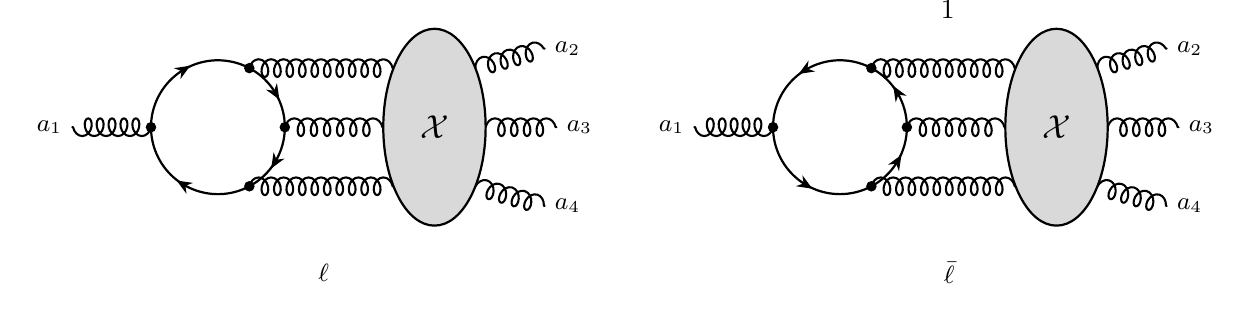
\begin{tikzpicture}[fd]
  \def\fdr{0.85}
  % #1: xshift; #2: 1 = clockwise, 0 = counterclockwise; #3: panel label
  \def\fdEmbed#1#2#3{%
    \begin{scope}[xshift=#1]
      \ifnum#2=1
        \draw[quark] (180:\fdr) arc[start angle=180,end angle=62,radius=\fdr];
        \draw[quark] (62:\fdr) arc[start angle=62,end angle=0,radius=\fdr];
        \draw[quark] (0:\fdr) arc[start angle=0,end angle=-62,radius=\fdr];
        \draw[quark] (-62:\fdr) arc[start angle=-62,end angle=-180,radius=\fdr];
      \else
        \draw[quark] (62:\fdr) arc[start angle=62,end angle=180,radius=\fdr];
        \draw[quark] (0:\fdr) arc[start angle=0,end angle=62,radius=\fdr];
        \draw[quark] (-62:\fdr) arc[start angle=-62,end angle=0,radius=\fdr];
        \draw[quark] (-180:\fdr) arc[start angle=-180,end angle=-62,radius=\fdr];
      \fi
      \draw[gluon] (180:\fdr) -- (-1.85,0) node[left]{$a_1$};
      \draw[gluon] (62:\fdr) -- (2.23,0.75);
      \draw[gluon] (0:\fdr) -- (2.1,0);
      \draw[gluon] (-62:\fdr) -- (2.23,-0.75);
      \foreach \ang in {180,62,0,-62} \node[vertex] at (\ang:\fdr) {};
      \draw[gluon] (3.27,0.75) -- (4.15,1.0) node[right]{$a_2$};
      \draw[gluon] (3.4,0) -- (4.3,0) node[right]{$a_3$};
      \draw[gluon] (3.27,-0.75) -- (4.15,-1.0) node[right]{$a_4$};
      \draw[blob] (2.75,0) ellipse[x radius=0.65cm,y radius=1.25cm];
      \node[font=\large] at (2.75,0) {$\mathcal X$};
      \node at (1.2,-1.85) {#3};
    \end{scope}}
  \fdEmbed{0cm}{1}{取向 $\ell$}
  \fdEmbed{7.9cm}{0}{反向圈 $\bar\ell$}
\end{tikzpicture}
\caption{把一个夸克圈嵌入任意 Feynman 图。两图的唯一差别是这个夸克圈的取向（费米子箭头方向）；
图的其余部分 $\mathcal X$（包括其中的一切顶点、传播子与其他圈）完全不变。图中只反转了一个圈；\cref{def:rho}的对合 $\rho$ 把一个缩并的\emph{全部}夸克圈同时反向，
\cref{lem:thmII-rho-value}给出 $W$ 与 $\rho W$ 之值的精确关系（只反转一个圈所得的两图之间一般没有这样的关系，见\cref{rem:thmII-orbits}）。}
\label{fig:embedding}
\end{figure}

%% ----------------------------------------------------------------------
\subsection{关键引理}\label{sec:thmII-lemma}

\begin{lemma}[$\rho$ 下缩并之值的变换]\label{lem:thmII-rho-value}
设\cref{thm:furry-allorders}中的假设 (H1)--(H3) 成立（正规化的条件见\cref{def:reg-hypotheses}），且夸克圈上的顶点都是 (V1)--(V3) 型
（夸克线上还有其他 C~本征顶点时，例如格点微扰论的顶点，见\cref{rem:thmII-general-vertices}：那里\cref{eq:thmII-rho-value}照样成立，\cref{eq:thmII-CK}的分解形式则一般不成立）。
固定 $\nu$ 与插入的味道指派 $\boldsymbol f$，并记 $\eta=\prod_{j=1}^m\eta_j$。则对每个完全 Wick 缩并 $W\in\mathcal W_\nu$ 与\cref{lem:setup-factorization}中的每个 $s$，
\begin{equation}\label{eq:thmII-CK}
C_s(\rho W)=(-1)^{k(W)}\,\Rop\,C_s(W),\qquad K_s(\rho W)=(-1)^{k(W)}\,\eta\,K_s(W),
\end{equation}
从而
\begin{equation}\label{eq:thmII-rho-value}
\operatorname{val}(\rho W)=\Bigl(\prod_{j=1}^m\eta_j\Bigr)\,\Rop\operatorname{val}(W),
\end{equation}
其中 $\Rop$ 对 $\operatorname{val}(W)$ 的每一个外伴随指标（外胶子场、外鬼场与外反鬼场的色指标）各作用一个 $R$。
特别地，若 $W$ 的每个闭合夸克圈的长度都不超过 $2$（即 $\rho W=W$），则 $\operatorname{val}(W)=\eta\,\Rop\operatorname{val}(W)$。
\end{lemma}

\begin{proof}
\emph{第一步（单个圈的色迹）。}设 $\ell=(i_1\,i_2\cdots i_k)$ 是 $W$ 的一个闭合夸克圈，色迹 $\tau_\ell:=\Tr(M_{i_1}M_{i_2}\cdots M_{i_k})$，
其中 (V1) 型顶点的 $M=T^a$，(V2)、(V3) 型顶点的 $M=\mathbb 1$。在 $\rho W$ 中这个圈换成 $\bar\ell$，由\cref{eq:setup-reversed}与\cref{lem:thmI-transpose}，
\[
\tau_{\bar\ell}=\Tr\bigl(M_{i_1}M_{i_k}M_{i_{k-1}}\cdots M_{i_2}\bigr)=\Tr\bigl(M_{i_1}^{\tp}M_{i_2}^{\tp}\cdots M_{i_k}^{\tp}\bigr).
\]
由\cref{def:phi-R}，$(T^a)^{\tp}=-\varphi(T^a)=-R^{ab}T^b$，而 $\mathbb 1^{\tp}=\mathbb 1$。代入后提出纯数因子，得
\begin{equation}\label{eq:thmII-tau}
\tau_{\bar\ell}=(-1)^{k_g(\ell)}\,\Rop_{(\ell)}\tau_\ell ,
\end{equation}
其中 $\Rop_{(\ell)}$ 对 $\tau_\ell$ 的每个伴随指标（$\ell$ 上各 (V1) 型顶点所连胶子的色指标）各作用一个 $R$；只含 (V1) 型顶点时这就是\cref{eq:color-reversal}（$r=F$）。
推导没有用到 $\bar\ell\neq\ell$，所以\cref{eq:thmII-tau}对 $k\le2$ 也成立，此时它是一致性条件：$k_g(\ell)=1$ 时两边因 $\Tr T^a=0$ 而为零，
$k_g(\ell)=2$ 时它就是 $\frac12\delta^{ab}$ 的 C~偶性，$k_g(\ell)=0$ 时 $\tau_\ell=N$ 不带指标。

\emph{第二步（色网络）。}按\cref{lem:setup-factorization}，$C_s(W)=\mathfrak c_W\bigl(\bigotimes_vb_v\otimes\bigotimes_\ell\tau_\ell\bigr)$，其中 $\ell$ 取遍 $W$ 的全部闭合夸克圈；
$b_v$ 取遍胶子与鬼场传播子的 $\delta^{ab}$、三胶子顶点与鬼场--胶子顶点的 $f^{abc}$、四胶子顶点所选的 $f^{abe}f^{cde}$ 型色结构（由 $s$ 决定）以及胶子与鬼场部分的正规化与抵消项所引入的顶点的色张量；
$\mathfrak c_W$ 是由 $P$、$\sigma$ 与各圈的顶点集合决定的缩并方式（每对缩并的指标用 $\delta$ 求和），剩下的自由指标就是外伴随指标。
由\cref{lem:setup-factorization}(iii)，$\mathfrak c_W$ 对 $W$ 与 $\rho W$ 相同；由\cref{lem:building-blocks}（正规化与抵消项所引入的顶点还用到 (R3) 与 (H3)），$\Rop b_v=b_v$。于是由\cref{eq:thmII-tau}，
\begin{align*}
C_s(\rho W)&=\mathfrak c_W\Bigl(\bigotimes_vb_v\otimes\bigotimes_\ell(-1)^{k_g(\ell)}\Rop_{(\ell)}\tau_\ell\Bigr)
=(-1)^{k(W)}\,\mathfrak c_W\Bigl(\Rop\Bigl[\bigotimes_vb_v\otimes\bigotimes_\ell\tau_\ell\Bigr]\Bigr)\\
&=(-1)^{k(W)}\,\Rop\,\mathfrak c_W\Bigl(\bigotimes_vb_v\otimes\bigotimes_\ell\tau_\ell\Bigr)=(-1)^{k(W)}\,\Rop\,C_s(W),
\end{align*}
方括号内的 $\Rop$ 作用于张量积的全部指标。第三个等号是\cref{lem:contraction}(i) 的证明中的事实：由 $R^{\tp}R=\mathbb 1$，用 $\delta$ 缩并一对指标与 $\Rop$ 对易，
所以先对全部指标作用 $\Rop$ 再缩并，等于先缩并、再对剩下的外指标作用 $\Rop$。这证明了\cref{eq:thmII-CK}的第一式。

\emph{第三步（Dirac 因子）。}按\cref{lem:setup-factorization}(ii)，$K_s(W)$ 是以下因子之积对顶点位置的积分：$1/\nu!$；胶子与鬼场传播子；
三胶子、四胶子、鬼场--胶子顶点以及胶子与鬼场部分的正规化与抵消项所引入的顶点的 Lorentz 部分（连同各自的耦合常数、抵消项系数与因子 $\ii$）；鬼场符号 $\operatorname{sgn}_{\mathrm{gh}}(\sigma)$；
每个闭合夸克圈的因子 $-\bigl(\prod_{v\in\ell}\kappa_v\bigr)K_\ell$（\cref{eq:loop-factorized}）。
这里 $\ii^{|\nu|}$ 的每个因子 $\ii$ 已按 Feynman 规则并入相应的相互作用顶点，夸克圈上各顶点的 $\kappa_v$ 为：夸克--胶子顶点 $\kappa_v=\ii g$，其抵消项 $\kappa_v=\delta_{1F}\ii g$；
插入 $O_j$ 的 $\kappa_v$ 即味道权重 $\kappa_j^{(f_j)}$；(V3) 型顶点 $\kappa_v=1$，其因子 $\ii$ 已含在\cref{eq:thmII-X}的 $X$ 中。
除 $K_\ell$ 外，这些因子只依赖于 $\nu$、$\boldsymbol f$、$P$、$\sigma$ 与各圈的顶点集合，在 $\rho$ 下不变；唯一改变的是 $K_\ell\mapsto K_{\bar\ell}$。
由\cref{prop:loop-reversal}（坐标空间形式见\cref{eq:loop-reversal}），并对 (V3) 型顶点使用\cref{rem:thmI-derivative}，
\begin{equation}\label{eq:thmII-K}
K_{\bar\ell}=\Bigl(\prod_{v\in\ell}\eta_v\Bigr)K_\ell,\qquad
\eta_v=\begin{cases}-1, & v\ \text{为 (V1) 型顶点},\\ \eta_j, & v\ \text{为插入}\ O_j,\\ +1, & v\ \text{为 (V3) 型顶点},\end{cases}
\end{equation}
它在 (R1) 之下对一切顶点位置逐点成立。（对 (V3) 型顶点，反序把对称化导数 $\overleftrightarrow{\partial_\mu}$ 所作用的两条传播子互换，
由于 $\overleftrightarrow{\partial_\mu}$ 对二者反对称，这给出一个负号；$\Cconj{\gamma^\mu}=-\gamma^\mu$ 再给出一个负号；两个负号相消，$\delta_m$ 项不受影响，
故 $X$ 逐点不变——这就是\cref{eq:thmII-X}的坐标空间形式。）由 (d)，每个 (V1) 型顶点与每个插入都恰在一个圈上，故
$\prod_\ell\prod_{v\in\ell}\eta_v=(-1)^{k(W)}\eta$，即 $K_s(\rho W)$ 与 $K_s(W)$ 的被积函数逐点只差因子 $(-1)^{k(W)}\eta$。
（第一步与第三步合起来正是\cref{thm:furry-single}的\cref{eq:master}：$L_{\bar\ell}$ 等于把 $\ell$ 上每个色矩阵 $M$ 换成 $M^{\mathsf c}=\eta_vM^{\tp}$ 后的 $L_\ell$；
这里把色部分与 Dirac 部分分开写，是为了与\cref{lem:setup-factorization}的分解相对应。）

\emph{第四步（积分）。}若正规化是通过满足 (R1) 坐标空间形式、且在顶点重合处也有定义的正规化传播子实现的（\cref{rem:reg-selfreverse}），第三步的逐点等式在对顶点位置积分后仍成立，即得\cref{eq:thmII-CK}的第二式。
若在动量空间中计算（例如维数正规化），对 $\rho W$ 中每个反向的圈采用\emph{镜像动量配置}——几何上同一条夸克线在 $W$ 与 $\rho W$ 中携带同一个物理动量
（因而沿新箭头的动量反号），其余各线的动量照搬（两者的无向图相同，动量守恒自动满足）。于是作为圈动量的函数，每个长度 $\ge3$ 的圈的 Dirac 因子逐点满足\cref{eq:thmII-K}（\cref{eq:loop-reversal-mom}，\cref{eq:thmI-derivative}），其余因子相同。
由 (R2)，积分之后这些关系仍成立：在 (R2) 的第二种形式下，$\rho W$ 本来就采用镜像配置，并对同一组圈动量施加同一正规化；在第一种形式下，积分与动量配置无关，
因为 $\rho W$ 的任一配置与镜像配置只相差圈动量的平移（可含其他圈动量）与反射。
长度 $\le2$ 的圈不被 $\rho$ 改变，在 $W$ 与 $\rho W$ 中采用同一配置，其因子完全相同，所需的只是一致性条件 $K_\ell=(\prod_{v\in\ell}\eta_v)K_\ell$（对该圈的子积分而言）：
它在 $\prod_{v\in\ell}\eta_v=+1$ 时平凡；在 $\prod_{v\in\ell}\eta_v=-1$ 时要求 $K_\ell=0$。这在坐标空间中对上述正规化传播子由 (R1) 逐点给出（\cref{sec:dirac-loop}中的“短圈”一段）。在动量空间中，由\cref{eq:loop-reversal-mom}与\cref{eq:thmI-derivative}（取 $\bar\ell=\ell$），
该圈的被积函数在镜像重参数化（长度为 $1$ 时 $q\to-q$；长度为 $2$、两条线携带 $q$ 与 $q+p$ 时 $q\to-q-p$）下乘以 $\prod_{v\in\ell}\eta_v=-1$，
而由 (R2) 该圈积分在这一重参数化下不变，故 $K_\ell=0$（\cref{rem:reg-selfreverse}；维数正规化满足之）。
（若此时 $k_g(\ell)=1$，则 $\tau_\ell=\Tr T^a=0$，这个缩并之值本来就为零。）合起来即得\cref{eq:thmII-CK}的第二式。

\emph{第五步（合并）。}$\Rop$ 是线性的，只作用于色指标，与不带色指标的 $K_s(W)$ 交换，故
\[
\operatorname{val}(\rho W)=\sum_s(-1)^{k(W)}\Rop C_s(W)\cdot(-1)^{k(W)}\eta\,K_s(W)=\eta\,\Rop\sum_sC_s(W)K_s(W)=\eta\,\Rop\operatorname{val}(W).
\]
两个 $(-1)^{k(W)}$ 分别来自色空间中的转置 $(T^a)^{\tp}=-R^{ab}T^b$ 与 Dirac 空间中的 $\Cconj{\gamma^\mu}=-\gamma^\mu$，在乘积中相消，与\cref{sec:thmI}的符号核对相同。
引理的最后一句是 $\rho W=W$ 时的特例。
\end{proof}

\begin{remark}[一般的 C~本征顶点]\label{rem:thmII-general-vertices}
证明只用到每个顶点在电荷共轭下是本征的。若还有其他局域顶点 $v$（例如格点微扰论的夸克线顶点、复合算符的抵消项，或含胶子场的算符插入）在\cref{eq:C-fields}下满足 $v\mapsto\epsilon_vv$，
并且含 $r\ge2$ 个胶子场的顶点使用对其胶子槽位对称化的 Feynman 规则，则同样的证明给出 $\operatorname{val}(\rho W)=(\prod_v\epsilon_v)\,\Rop\operatorname{val}(W)$，
其中 $\prod_v$ 取遍全部顶点（拉氏量及其抵消项的顶点 $\epsilon_v=+1$，插入 $O_j$ 的 $\epsilon_v=\eta_j$）。
这里“对称化”指对 $r$ 个槽位的 $r!$ 种指派取平均，色指标、Lorentz 指标与动量随槽位一起置换（如\cref{lem:setup-factorization}中平均后的 $\mathcal L_4$；
格点微扰论中由 $U_{x,\mu}$ 展开得到的多胶子顶点也可以这样书写）。理由是：含夸克场的顶点 $\bar\psi(\Gamma\otimes M)\psi$（可乘以若干胶子场）位于一个夸克圈上，
由\cref{lem:bilinear}与 $A^a\to R^{ab}A^b$，把它的（对称化的）系数按 Dirac 部分与色部分的 C~本征分量展开（各项计入\cref{lem:setup-factorization}的求和指标 $s$）之后，
每一项在第二、三步中贡献的符号之积都是 $\epsilon_v$；不含夸克场的顶点的 $\epsilon_v$ 是其（对称化的）色张量的 C~宇称。
例如 $\bar\psi\,\Gamma T^a\psi\,A^a\mapsto\eta_\Gamma\,\bar\psi\,\Gamma(T^a)^{\tp}\psi\,R^{ab}A^b=-\eta_\Gamma R^{ac}R^{ab}\,\bar\psi\,\Gamma T^c\psi\,A^b=-\eta_\Gamma\,\bar\psi\,\Gamma T^b\psi\,A^b$。

对称化不可省略：$v\mapsto\epsilon_vv$ 是场的多项式之间的等式，只约束系数张量中对胶子槽位对称的部分，而带标号的展开区分各个槽位。
对有序的单项式 $\bar\psi(\Gamma\otimes T^{a_1}\cdots T^{a_r})\psi\,A^{a_1}\cdots A^{a_r}$，有 $(T^{a_1}\cdots T^{a_r})^{\tp}=(-1)^rR^{a_1b_1}\cdots R^{a_rb_r}\,T^{b_r}\cdots T^{b_1}$，即转置把槽位反序。
例如，C~偶的顶点
\[
\bar\psi(\gamma^\mu\gamma^\nu\otimes T^aT^b)\psi\,A^a_\mu A^b_\nu
\]
与一个夸克--胶子顶点 $\gamma^\rho\otimes T^c$ 组成长度为 $2$ 的圈（$\rho W=W$），三个胶子都接到外线时，
$\operatorname{val}(W)-\Rop\operatorname{val}(W)$ 的被积函数正比于 $\frac12d^{abc}\,\TrD\bigl[\gamma^\mu\gamma^\nu\SF(z)\gamma^\rho\SF(-z)\bigr]$（$z$ 为两顶点之差），它在 $m\neq0$ 时一般不为零；
只有与交换这两个胶子槽位的缩并相加后，结果才是 C~偶的。若不对称化（对夸克线顶点，即不满足 (R1) 中的这一约定），槽位置换仍是 $\mathcal W_\nu$ 上与 $\rho$ 对易的双射（与性质 (iii) 同理），
对它们求平均等于改用对称化的顶点，所以\cref{thm:furry-allorders}的求和形式不变；但其中“更强地”一句所说的子集还须在这些槽位置换下封闭。
\end{remark}

%% ----------------------------------------------------------------------
\subsection{主定理 II 及其证明}\label{sec:thmII-main}

\begin{theorem}[主定理 II：微扰 QCD 中任意阶的 Furry 定理]\label{thm:furry-allorders}
假设：(H1) 规范固定的 QCD 拉氏量\cref{eq:lagrangian}（任意 $\xi$，任意 $n_f$ 个味道，质量为实数）；
(H2) 维数正规化（\cref{def:dimreg-trace}）或任何满足\cref{def:reg-hypotheses}中 (R1)--(R3) 的正规化；
(H3) 以 C~不变的抵消项进行重整化（例如 $\overline{\mathrm{MS}}$ 方案）。
设 $G$ 为 $n_A$ 个胶子场、$n_c$ 个鬼场、$n_{\bar c}$ 个反鬼场以及 $m$ 个味对角的色单态算符
$O_j=\sum_f\kappa_j^{(f)}\bar\psi_f\Gamma_j\psi_f$（$\Gamma_j$ 的 C~宇称为 $\eta_j$）的编时 Green 函数（完全的、连通的、截腿的或单粒子不可约的均可）。
则在 $g$ 的每一阶，对一切时空坐标（或动量）与 Lorentz 指标，
\begin{equation}\label{eq:selection-rule}
\Rop\,G=\Bigl(\prod_{j=1}^{m}\eta_j\Bigr)\,G ,
\end{equation}
其中 $\Rop$ 表示对 $G$ 的每一个伴随色指标各作用一个 $R$。更强地，对任何在 $\rho$ 下封闭的缩并子集求和，\cref{eq:selection-rule}同样成立。
\end{theorem}

关于假设的两点说明。(1) 在维数正规化中，“$\Gamma_j$ 的 C~宇称为 $\eta_j$”应理解为 $\Cconj{\Gamma_j}=\eta_j\Gamma_j$ 在\cref{def:dimreg-trace}的形式代数中成立：
对 $\mathbb 1$、$\gamma^\mu$、$\sigma^{\mu\nu}$ 这是自动的，轴矢流须用对称化的顶点（\cref{sec:reg-gamma5}）。
(2) 若色单态算符需要重整化，(H3) 也包括它们的抵消项：单个插入的抵消项须与 $O_j$ 有相同的 C~宇称，
多个插入的接触抵消项（源的多项式，可乘以局域场算符）须具有相应插入的 C~宇称之积（\cref{rem:thmII-general-vertices}，\cref{rem:reg-composite}）。

\begin{proof}
记 $\eta=\prod_j\eta_j$。

\emph{第一步（完全 Green 函数）。}固定 $\nu$ 与 $\boldsymbol f$。$\mathcal W_\nu$ 是有限集，$\rho$ 是它到自身的双射（\cref{def:rho}），
于是由\cref{lem:thmII-rho-value}（夸克线上有 (V1)--(V3) 以外的 C~本征顶点时，例如格点微扰论，改用\cref{rem:thmII-general-vertices}；那里的 $\prod_v\epsilon_v$ 由 (R1)、(R3) 与 (H3) 等于 $\eta$），
\begin{equation}\label{eq:thmII-sum}
\sum_{W\in\mathcal W_\nu}\operatorname{val}(W)=\sum_{W\in\mathcal W_\nu}\operatorname{val}(\rho W)=\eta\,\Rop\sum_{W\in\mathcal W_\nu}\operatorname{val}(W).
\end{equation}
每个内部顶点（包括抵消项顶点）至少带一个因子 $g$，所以 $g$ 的固定阶 $t$ 只涉及有限多个 $\nu$；对它们与 $\boldsymbol f$ 求和，得 $\Rop\mathcal N^{(t)}=\eta\,\mathcal N^{(t)}$。
由\cref{lem:setup-vacuum}（取 $\mathfrak L=\Rop$），$\Rop G^{(r)}=\eta\,G^{(r)}$ 对一切 $r$ 成立。$\Rop$ 只作用于色指标，与对坐标的 Fourier 变换交换，所以动量空间中的 Green 函数同样满足\cref{eq:selection-rule}。

\emph{第二步（在 $\rho$ 下封闭的子集）。}若 $\mathcal S\subseteq\mathcal W_\nu$ 满足 $\rho(\mathcal S)=\mathcal S$，则 $\rho|_{\mathcal S}$ 是双射，\cref{eq:thmII-sum}的计算逐字给出
$\Rop\sum_{W\in\mathcal S}\operatorname{val}(W)=\eta\sum_{W\in\mathcal S}\operatorname{val}(W)$，这就是“更强地”的断言。最小的这种子集是 $\rho$ 的轨道 $\{W,\rho W\}$；
由性质 (i)，一切由无向图定义的子集（连通的、不含真空分量的、单粒子不可约的缩并）都在 $\rho$ 下封闭。

\emph{第三步（连通 Green 函数）。}设 $E$ 为外场的集合，对每个子集 $B\subseteq E$ 记 $G(B)$ 为 $B$ 中外场的完全 Green 函数，$\eta_B$ 为 $B$ 中色单态算符的 C~宇称之积。由矩--累积量关系，
\[
G_c(E)=\sum_{\Pi}c_\Pi\prod_{B\in\Pi}G(B),
\]
$\Pi$ 取遍 $E$ 的划分，$c_\Pi$ 是只依赖于划分（以及外鬼场与外反鬼场重排的 Grassmann 符号）的数。由第一步，$\Rop G(B)=\eta_BG(B)$；$\Rop$ 在乘积上逐个因子作用，
而 $\prod_{B\in\Pi}\eta_B=\eta$，故 $\Rop G_c(E)=\eta\,G_c(E)$。

\emph{第四步（截腿 Green 函数）。}截腿是在每条外胶子腿、外鬼场腿与外反鬼场腿上乘以相应的完全两点函数之逆（或树图传播子之逆）。由第一步（$n_A=2$，$m=0$），
胶子的完全两点函数 $D$ 满足 $\Rop D=D$；把 $D$ 看作色指标、Lorentz 指标与动量上的矩阵，这就是 $RDR=D$（$R$ 对称），因而 $RD^{-1}R=D^{-1}$，即 $RD^{-1}=D^{-1}R$。
鬼场两点函数同理，树图传播子正比于 $\delta^{ab}$，亦然。截腿函数 $G_{\mathrm{amp}}=\bigl(\prod_iD_i^{-1}\bigr)G_c$（每条腿一个因子）的每条腿上的 $R$ 可以穿过 $D_i^{-1}$ 作用到 $G_c$ 上，
故 $\Rop G_{\mathrm{amp}}=\bigl(\prod_iD_i^{-1}\bigr)\Rop G_c=\eta\,G_{\mathrm{amp}}$。

\emph{第五步（单粒子不可约函数）。}引入胶子源 $J$、鬼场源 $\zeta,\bar\zeta$ 与复合算符源 $K_j$，令 $\mathcal E[J,\zeta,\bar\zeta,K]$ 为连通 Green 函数的生成泛函（形式幂级数）。
第三步对一切外场组合成立，比较 Taylor 系数可知这等价于
\begin{equation}\label{eq:thmII-W}
\mathcal E[J,\zeta,\bar\zeta,K]=\mathcal E[RJ,R\zeta,R\bar\zeta,\eta K],
\end{equation}
其中 $(RJ)^a_\mu(x)=R^{ab}J^b_\mu(x)$，$\eta K$ 表示 $K_j\mapsto\eta_jK_j$（对一个源每求一次导数产生一个 $R$，而 $R$ 是对称的）。
单粒子不可约函数的生成泛函是 Legendre 变换 $\Gamma[\Phi,K]=\mathcal E[J,K]-J\cdot\Phi$（鬼场同理，对 Grassmann 源用左导数），其中 $J=J[\Phi,K]$ 由 $\Phi=\delta\mathcal E/\delta J$ 决定。
对\cref{eq:thmII-W}求导得 $\Phi[RJ,\eta K]=R\,\Phi[J,K]$，从而 $J[R\Phi,\eta K]=R\,J[\Phi,K]$，于是由 $R^{\tp}R=\mathbb 1$，
\[
\Gamma[R\Phi,\eta K]=\mathcal E[RJ,\eta K]-(RJ)\cdot(R\Phi)=\mathcal E[J,K]-J\cdot\Phi=\Gamma[\Phi,K].
\]
对 $\Phi$ 与 $K$ 求导并令其为零即得结论。（在微扰论中 Legendre 变换逐阶存在，因为规范固定后的自由二次型可逆，且 $\langle A^a_\mu\rangle=\langle c^a\rangle=\langle\bar c^a\rangle=0$。）

\emph{第六步（抵消项）。}在 $\overline{\mathrm{MS}}$ 方案中（\cref{prop:reg-dimreg}），抵消项顶点或是 (V1)、(V3) 型的夸克线顶点，或是色张量 C~偶的胶子、鬼场顶点（\cref{lem:building-blocks}），都已包含在\cref{lem:thmII-rho-value}中；
(H3) 允许的其他抵消项顶点（其他方案中 C~不变的局域抵消项，例如格点微扰论中含多个胶子场的夸克线抵消项顶点，以及与 $O_j$ 有相同 C~宇称的复合算符抵消项）由\cref{rem:thmII-general-vertices}处理，
多个插入的接触抵消项见\cref{rem:reg-composite}。因此以上各步对重整化的 Green 函数逐阶成立。
\end{proof}

\begin{remark}[逐轨道的细化；鬼场圈]\label{rem:thmII-orbits}
设 $W$ 有 $q$ 个长度 $\ge3$ 的闭合夸克圈 $\ell_1,\dots,\ell_q$，对 $I\subseteq\{1,\dots,q\}$ 令 $\rho_IW$ 为只反向 $\{\ell_i\}_{i\in I}$ 所得的缩并。
由于 $\ell_i\neq\bar\ell_i$，$(\mathbb Z_2)^q$ 经由 $I\mapsto\rho_I$ 在轨道 $\mathcal O(W)=\{\rho_IW\}_I$ 上自由且可迁地作用，$|\mathcal O(W)|=2^q$。
$\operatorname{val}(\rho_IW)$ 中与夸克圈无关的部分（记作 $\mathcal X_{P,\sigma}$）不依赖于 $I$，故（对长度 $\ge3$ 的圈采用镜像配置）
\[
\sum_{W'\in\mathcal O(W)}\operatorname{val}(W')=\mathcal X_{P,\sigma}\otimes\prod_{|\ell|\le2}L_\ell\ \prod_{i=1}^{q}\bigl(L_{\ell_i}+L_{\bar\ell_i}\bigr)
\]
（这是被积函数之间的等式，积分在其后），$\otimes$ 表示按 $\mathfrak c_W$ 缩并色指标。由\cref{thm:furry-single}与\cref{cor:singlet}（(V3) 型顶点按\cref{rem:thmI-derivative}处理），$L_{\ell_i}+L_{\bar\ell_i}=-(\prod\kappa)K_{\ell_i}\cdot2\,\mathcal P_{\eta(\ell_i)}\tau_{\ell_i}$，$\eta(\ell)$ 为 $\ell$ 上插入的 C~宇称之积；
短圈的 $L_\ell$ 由\cref{eq:thmII-tau}与\cref{eq:thmII-K}满足 $\Rop L_\ell=\eta(\ell)L_\ell$（$\prod_{v\in\ell}\eta_v=-1$ 时 $L_\ell=0$：在坐标空间中这要求正规化传播子在顶点重合处也有定义，在动量空间中这要先对该圈的圈动量积分并用 (R2)；见\cref{lem:thmII-rho-value}的第四步）。
所以每个圈上 C~宇称与 $\eta(\ell)$ 相反的部分 $\mathcal P_{-\eta(\ell)}\tau_\ell$ \emph{逐圈}相消，而 $\mathcal X_{P,\sigma}$ 的色张量都是 C~偶的，由\cref{lem:contraction}(i)，
轨道之和满足\cref{eq:selection-rule}；由于 $\mathcal O(W)$ 在 $\rho=\rho_{\{1,\dots,q\}}$ 下封闭，这也是“更强地”断言的特例。只对一部分圈求取向之和（例如 $\{W,\rho_{\{1\}}W\}$）一般\emph{不}给出 C~本征的结果。

鬼场圈与胶子圈的色因子是 $f^{abc}$ 的网络（\cref{eq:setup-ghost-loop}），对每一种取向分别是 C~偶的（\cref{lem:contraction}(iii)，\cref{fig:adjoint-loops}），
所以鬼场圈不需要把两种取向配对（\cref{sec:setup-loops}末段），证明中也从未用到二者的关系；因此在纯 Yang--Mills 理论（$n_f=0$）中\emph{每一个}缩并都是 C~偶的，C~奇的色张量只能来自夸克圈。
\end{remark}

\begin{figure}[htbp]
\centering
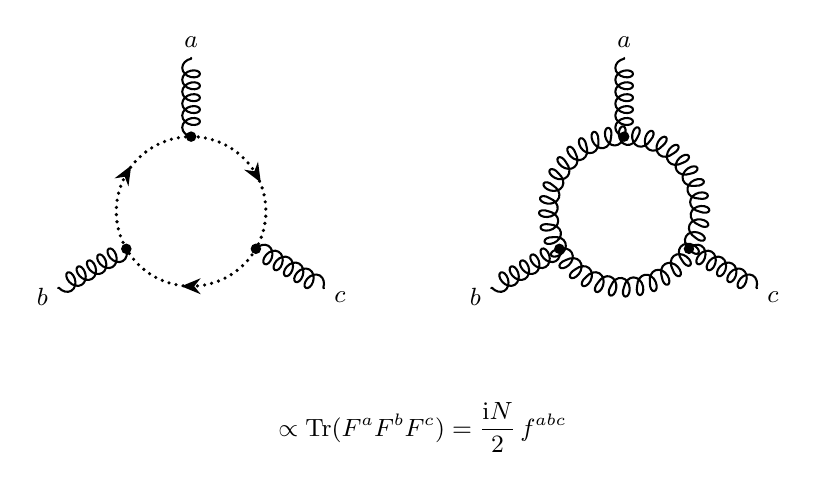
\begin{tikzpicture}[fd]
  \def\fdR{0.95}\def\fdL{1.0}
  \begin{scope}
    \draw[ghost] (90:\fdR) arc[start angle=90,end angle=-30,radius=\fdR];
    \draw[ghost] (-30:\fdR) arc[start angle=-30,end angle=-150,radius=\fdR];
    \draw[ghost] (210:\fdR) arc[start angle=210,end angle=90,radius=\fdR];
    \draw[gluon] (90:\fdR) -- (90:\fdR+\fdL) node[above]{$a$};
    \draw[gluon] (210:\fdR) -- (210:\fdR+\fdL) node[anchor=30]{$b$};
    \draw[gluon] (330:\fdR) -- (330:\fdR+\fdL) node[anchor=150]{$c$};
    \foreach \ang in {90,210,330} \node[vertex] at (\ang:\fdR) {};
    \node at (0,-2.0) {鬼场圈};
  \end{scope}
  \begin{scope}[xshift=5.5cm]
    \draw[gluon loop=3] (90:\fdR) arc[start angle=90,end angle=450,radius=\fdR];
    \draw[gluon] (90:\fdR) -- (90:\fdR+\fdL) node[above]{$a$};
    \draw[gluon] (210:\fdR) -- (210:\fdR+\fdL) node[anchor=30]{$b$};
    \draw[gluon] (330:\fdR) -- (330:\fdR+\fdL) node[anchor=150]{$c$};
    \foreach \ang in {90,210,330} \node[vertex] at (\ang:\fdR) {};
    \node at (0,-2.0) {胶子圈};
  \end{scope}
  \node at (2.75,-2.75) {色结构 $\propto \Tr(F^aF^bF^c)=\dfrac{\ii N}{2}\,f^{abc}$};
\end{tikzpicture}
\caption{三胶子函数中的鬼场圈与胶子圈。圈上传播的是伴随表示的场（鬼场或胶子），其色因子正比于伴随表示生成元 $(F^a)_{bc}=-\ii f^{abc}$ 的迹
（\cref{eq:setup-ghost-loop}，\cref{eq:color-adjoint-trace}；其值见\cref{eq:app-traces-FFF}）。由于 $F^a$ 是纯虚反对称矩阵，$-(F^a)^{\tp}=F^a$：伴随表示与其共轭表示的生成元相同，
由\cref{lem:color-reversal}，伴随表示的迹是 C~偶的，因而只含 $f^{abc}$，不含 $d^{abc}$。鬼场圈的两种取向\emph{各自}是 C~偶的，无需配对。}
\label{fig:adjoint-loops}
\end{figure}

\begin{remark}[适用范围]\label{rem:thmII-scope}
(1) \emph{外夸克场。}若外场含 $\psi$ 或 $\bar\psi$，缩并中出现开放的夸克线，它不能在同一个 Green 函数内部反向；电荷共轭只给出夸克与反夸克 Green 函数之间的关系（\cref{rem:thmI-open-lines}），
而不是选择定则。例外是把 $q\bar q$ 对投影到确定 C~宇称的色单态（夸克偶素，\cref{sec:applications-quarkonium}）。
(2) \emph{动力学光子。}在 QCD$+$QED 中（若有带电轻子，把它们的圈一并纳入 $\rho$），每个光子--夸克顶点是 $\eta=-1$ 的色单态插入，每条内光子线连接两个这样的顶点，
同样的证明给出 $\Rop G=(-1)^{n_\gamma}(\prod_j\eta_j)G$，$n_\gamma$ 为外光子场的个数：这是\cref{cor:qed}的含义 (ii) 在任意阶的推广。
(3) \emph{$N=2$。}见\cref{rem:color-su2}(b) 与\cref{cor:selection}(b) 的最后一项。
\end{remark}

%% ----------------------------------------------------------------------
\subsection{选择定则}\label{sec:thmII-selection}

\begin{corollary}[选择定则]\label{cor:selection}
记 $\eta=\prod_j\eta_j$，并记 $n:=n_A+n_c+n_{\bar c}$ 为 $G$ 的外伴随指标的总数（外胶子、外鬼场与外反鬼场的色指标）。
\begin{enumerate}[label=(\alph*)]
\item （无需额外假设）对一切满足 $\Rop t=-\eta\,t$ 的 $n$ 指标色张量 $t$，$\langle t,G\rangle=0$。例如：$\eta=+1$、$n=3$ 时 $d^{abc}G^{abc}=0$（对三胶子函数即 $d^{abc}G^{abc}_{\mu\nu\rho}=0$）；
$\eta=+1$、$n=4$ 时 $G$ 与 $d^{abe}f^{cde}$、$d^{ace}f^{bde}$、$d^{ade}f^{bce}$ 正交。
\item 若 $G$ 还是整体 $\mathrm{SU}(N)$ 不变的（在 (H1)--(H3) 下成立），则
\begin{alignat*}{2}
&\eta=+1,\ n=3: &\quad& G^{abc}=f^{abc}\,\frac{f^{a'b'c'}G^{a'b'c'}}{N(N^2-1)};\\
&\eta=-1,\ n\le2: && G=0;\\
&\eta=-1,\ n=3,\ N\ge3: && G^{abc}=d^{abc}\,\frac{N\,d^{a'b'c'}G^{a'b'c'}}{(N^2-4)(N^2-1)};\\
&N=2,\ \eta=-1: && G\equiv0.
\end{alignat*}
\item 不含外胶子、外鬼场与外反鬼场（$n=0$）且 $\eta=-1$ 时 $G=0$：含奇数个 C~奇色单态流（例如电磁流）的 Green 函数在 $\alpha_s$ 的任意阶为零。
\end{enumerate}
\end{corollary}

$n$ 包括外鬼场与外反鬼场的指标，例如鬼场--胶子三点函数 $\langle c^a\bar c^bA^c_\mu\rangle$（$n=3$，$\eta=+1$）在任意阶正比于 $f^{abc}$；
而 $\langle\mathrm T\,J^\mu_{\mathrm{em}}A^a_\nu c^b\bar c^c\rangle$ 虽然只含一个外胶子，却有 $n=3$、$\eta=-1$：对 $N\ge3$，选择定则只要求它正比于 $d^{abc}$，并不要求它为零（$N=2$ 时它为零）。
（由鬼场数守恒，$n_c\neq n_{\bar c}$ 时 $G$ 本来就为零。）

\begin{proof}
\emph{(a)} 由\cref{lem:contraction}(ii) 与\cref{thm:furry-allorders}，
\[
\langle t,G\rangle=\langle\Rop t,\Rop G\rangle=\langle-\eta\,t,\ \eta\,G\rangle=-\eta^2\langle t,G\rangle=-\langle t,G\rangle ,
\]
故 $\langle t,G\rangle=0$；这里 $\langle t,G\rangle=t^{a_1\cdots a_n}G^{a_1\cdots a_n}$ 是双线性型，$G$ 的坐标（或动量）与 Lorentz 指标不参与缩并，只作为参数。
$\eta=+1$ 时可取任何 C~奇的 $t$：$d^{abc}$ 是 C~奇的（\cref{lem:R-properties}(iii)）；由\cref{lem:contraction}(i)，$d^{abe}f^{cde}$ 及其两个重排也是（C~奇乘 C~偶，再缩并一对指标）。
这一部分既不需要整体色不变性，也不需要不变张量的分类。

\emph{(b)} 先证整体不变性。在 (H1)--(H3) 下，每个 $C_s(W)$ 都是以下色张量的缩并：$\delta^{ab}$、$f^{abc}$、$f^{abe}f^{cde}$、色迹 $\Tr(M_{i_1}\cdots M_{i_k})$，
以及正规化与抵消项引入的色张量（由 (R1)、(R3) 是不变张量）。它们都是\cref{eq:color-invariance}意义下的不变张量（色迹见\cref{sec:color-invariants}），而 $\mathrm{Ad}_g$ 是实正交矩阵，所以与\cref{lem:contraction}(i) 的证明相同（把 $R$ 换成 $\mathrm{Ad}_g$），
用 $\delta$ 缩并保持不变性。于是在 $g$ 的每一阶，$G$ 在固定的坐标与 Lorentz 指标下属于 $\mathrm{Inv}_n$；连通、截腿与单粒子不可约函数同理。
\begin{itemize}[leftmargin=1.6em,itemsep=2pt,topsep=2pt]
\item $\eta=+1$，$n=3$。由\cref{lem:invariants}，$G^{abc}=f^{abc}X+d^{abc}Y$（$N=2$ 时无 $d^{abc}$ 项），$X,Y$ 是运动学函数。由\cref{eq:f-even-d-odd}，$(\Rop G)^{abc}=f^{abc}X-d^{abc}Y$，
故\cref{eq:selection-rule}要求 $d^{abc}Y=0$；$N\ge3$ 时 $d^{abc}\neq0$，于是 $Y=0$。用 $f^{abc}f^{abc}=N(N^2-1)$ 与 $f^{abc}d^{abc}=0$（\cref{lem:app-traces-contractions}）缩并，得 $X=f^{abc}G^{abc}/(N(N^2-1))$。
\item $\eta=-1$，$n\le2$。$n=0$：$G$ 不带色指标，$\Rop G=G=-G$，故 $G=0$。$n=1$：$\mathrm{Inv}_1=0$，故 $G=0$（这一情形不需要 C）。
$n=2$：由 Schur 引理（\cref{lem:invariants}）$G^{ab}=\delta^{ab}X$，$\delta^{ab}$ 是 C~偶的，故 $\Rop G=G=-G$，$G=0$——C~与 Schur 引理缺一不可。
\item $\eta=-1$，$n=3$，$N\ge3$。$G^{abc}=f^{abc}X+d^{abc}Y$，$(\Rop G)^{abc}=f^{abc}X-d^{abc}Y=-G^{abc}$ 给出 $X=0$；
用 $d^{abc}d^{abc}=(N^2-4)(N^2-1)/N$ 缩并得 $Y=N\,d^{abc}G^{abc}/((N^2-4)(N^2-1))$。
\item $N=2$，$\eta=-1$。由\cref{prop:su2}(i)，每个 $\mathrm{SU}(2)$ 不变张量都是 C~偶的，故 $\Rop G=G$；与 $\Rop G=-G$ 合起来得 $G=0$，对任意 $n$ 成立。
\end{itemize}
以上系数已对 $N=2,3,4,5$ 数值核验（包括 $R$ 不是对角矩阵的随机正交基）。

\emph{(c)} 没有外伴随指标时 $\Rop$ 是恒等映射，\cref{eq:selection-rule}化为 $G=\eta\,G=-G$，故 $G=0$；不需要整体色不变性。
\end{proof}

%% ----------------------------------------------------------------------
\subsection{例子}\label{sec:thmII-examples}

\begin{example}[三胶子顶点]\label{ex:thmII-3g}
由\cref{thm:furry-allorders}（单粒子不可约，$\eta=+1$）与\cref{cor:selection}(b)，完全的三胶子顶点在任意阶都只含 $f^{abc}$：
\begin{equation}\label{eq:thmII-3g}
\Gamma^{abc}_{\mu\nu\rho}(p_1,p_2,p_3)=f^{abc}\,\Gamma_{\mu\nu\rho}(p_1,p_2,p_3),\qquad
\Gamma_{\mu\nu\rho}=\frac{f^{a'b'c'}\Gamma^{a'b'c'}_{\mu\nu\rho}}{N(N^2-1)} .
\end{equation}
由 Bose 对称性与 $f^{abc}$ 的全反对称性，$\Gamma_{\mu\nu\rho}$ 在交换任意两条腿的 $(\mu,p)$ 时反号。树图值为 $gf^{abc}V_{\mu\nu\rho}$，单圈夸克圈的贡献见\cref{prop:triangle}。
不用不变张量的分类时仍有 $d^{abc}\Gamma^{abc}_{\mu\nu\rho}=0$（\cref{cor:selection}(a)）。Bose 对称性本身允许 $d^{abc}$ 乘以全对称的运动学张量（\cref{rem:tri-bose}），排除它的是 C。
\end{example}

\begin{example}[$\gamma^*\to gg$ 与 $\gamma^*\to ggg$]\label{ex:thmII-photon}
对电磁流 $J^\mu_{\mathrm{em}}=\sum_fQ_f\bar\psi_f\gamma^\mu\psi_f$（$\eta=-1$），由\cref{cor:selection}(b)，在 $\alpha_s$ 的任意阶
\begin{equation}\label{eq:thmII-photon}
\bigl\langle\mathrm T\,J^\mu_{\mathrm{em}}(x)\,A^a_\nu(y)\,A^b_\rho(z)\bigr\rangle=0,\qquad
\bigl\langle\mathrm T\,J^\mu_{\mathrm{em}}(x)\,A^a_\nu(y)\,A^b_\rho(z)\,A^c_\sigma(w)\bigr\rangle=d^{abc}\,\mathcal G^\mu{}_{\nu\rho\sigma}(x;y,z,w)
\end{equation}
（后者要求 $N\ge3$；$N=2$ 时它为零）。前者对离壳的胶子与任意虚光子成立，由它截腿得到的一切微扰振幅 $\gamma^*\to gg$ 为零；单圈时这是\cref{fig:mixed}(a) 中两图的相消，
任意阶则需同时用到 C~与 Schur 引理（\cref{tab:thmI-examples}）。后者说明 $\gamma^*\to ggg$ 的三个胶子处于 C~奇的 $d^{abc}$ 型色单态；$J/\psi\to ggg$ 的类似结论见\cref{prop:app-quarkonium}与\cref{rem:app-onium-allorders}。
\end{example}

\begin{example}[四胶子函数；只含色单态算符的函数]\label{ex:thmII-4g}
对 $\eta=+1$、$n=n_A=4$，\cref{cor:selection}(a) 给出 $G^{abcd}$ 与 $d^{abe}f^{cde}$、$d^{ace}f^{bde}$、$d^{ade}f^{bce}$ 正交；再用整体不变性与\cref{lem:invariants}，
$G$ 属于由三个 $\delta^{ab}\delta^{cd}$ 型与三个 $d^{abe}d^{cde}$ 型张量张成的 C~偶子空间（$N=3$ 时其间有一个线性关系\cref{eq:app-traces-su3-dd}，$N=2$ 时只有 $\delta^{ab}\delta^{cd}$ 型），
$f^{abe}f^{cde}$ 也可由它们表出（\cref{eq:app-traces-ff-dd}）：四胶子函数在任意阶都没有 $d^{abe}f^{cde}$ 型结构。对单粒子不可约的四胶子函数，单圈时这就是\cref{fig:boxes}中三对方框图各给出 $2\Real\Tr$（\cref{eq:thmI-box}）；
在连通函数中，夸克三角圈经一条内胶子接到树图三胶子顶点的单圈图（例如外胶子 $a,b$ 接在三角圈上）所含的 $\frac14d^{abe}f^{ecd}$ 项同样在两种取向之间相消。
另一方面，由\cref{cor:selection}(c)，在 $\alpha_s$ 的任意阶 $\langle J^\mu_{\mathrm{em}}\rangle=0$，三光子函数 $\langle\mathrm T\,J^\mu_{\mathrm{em}}J^\nu_{\mathrm{em}}J^\rho_{\mathrm{em}}\rangle=0$（QCD 修正下的 Furry 定理），
矢量流与标量密度的混合 $\langle\mathrm T\,J^\mu_{\mathrm{em}}(x)\,\bar\psi_f\psi_f(y)\rangle=0$，$\langle\mathrm T\,J_{\mathrm{em}}J_{\mathrm{em}}\,\bar\psi\sigma^{\mu\nu}\psi\rangle=0$（$\eta=(-1)^3$）；
而光--光散射 $\langle\mathrm T\,J_{\mathrm{em}}J_{\mathrm{em}}J_{\mathrm{em}}J_{\mathrm{em}}\rangle$ 与 VVA 三点函数（$\eta=+1$）不受约束。
\end{example}

%% ----------------------------------------------------------------------
\subsection{对称因子与自共轭图}\label{sec:thmII-symmetry}

%% ---- fig:thmII-selfconj (new) ----
\begin{figure}[htbp]
\centering
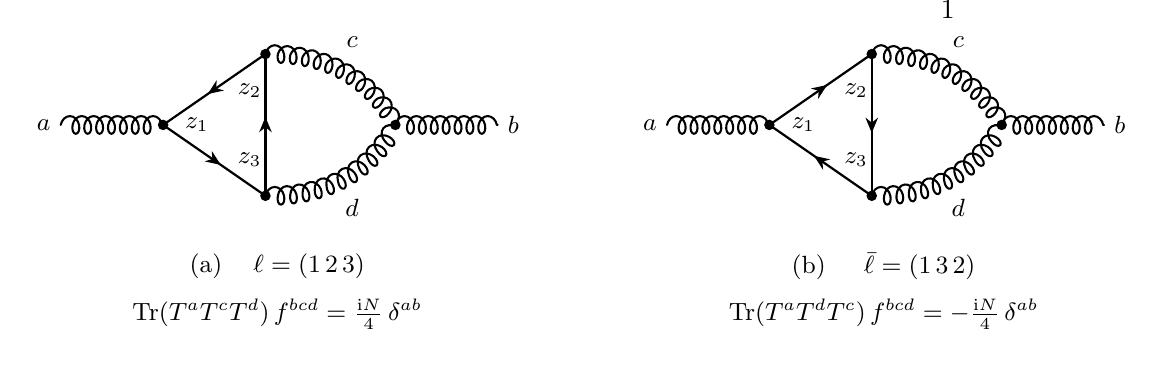
\begin{tikzpicture}[fd]
  % #1: xshift; #2: 1 = orientation \ell = (1 2 3) (fermion flow z2->z1, z3->z2, z1->z3), 0 = reversed;
  % #3: panel label; #4: colour factor
  \def\fdSelf#1#2#3#4{%
    \begin{scope}[xshift=#1]
      \coordinate (z1) at (-0.95,0); \coordinate (z2) at (0.35,0.9);
      \coordinate (z3) at (0.35,-0.9); \coordinate (y) at (2.0,0);
      \ifnum#2=1
        \draw[quark] (z2) -- (z1); \draw[quark] (z1) -- (z3); \draw[quark] (z3) -- (z2);
      \else
        \draw[quark] (z1) -- (z2); \draw[quark] (z2) -- (z3); \draw[quark] (z3) -- (z1);
      \fi
      \draw[gluon] (-2.25,0) node[left]{$a$} -- (z1);
      \draw[gluon] (z2) to[out=0,in=120] (y);
      \draw[gluon] (z3) to[out=0,in=240] (y);
      \draw[gluon] (y) -- (3.3,0) node[right]{$b$};
      \foreach \pp in {z1,z2,z3,y} \node[vertex] at (\pp) {};
      \node[inner sep=1pt] at (-0.52,0) {$z_1$};
      \node[inner sep=1pt] at (0.15,0.44) {$z_2$};
      \node[inner sep=1pt] at (0.15,-0.44) {$z_3$};
      \node at (1.45,1.05) {$c$};
      \node at (1.45,-1.05) {$d$};
      \node at (0.5,-1.8) {#3};
      \node at (0.5,-2.4) {#4};
    \end{scope}}
  \fdSelf{0cm}{1}{(a)\ 取向 $\ell=(1\,2\,3)$}{$\Tr(T^aT^cT^d)\,f^{bcd}=\tfrac{\ii N}{4}\,\delta^{ab}$}
  \fdSelf{7.7cm}{0}{(b)\ 反向圈 $\bar\ell=(1\,3\,2)$}{$\Tr(T^aT^dT^c)\,f^{bcd}=-\tfrac{\ii N}{4}\,\delta^{ab}$}
\end{tikzpicture}
\caption{一个自共轭图：两圈胶子自能中含夸克三角圈与三胶子顶点的贡献（$\ell$ 的顶点 $z_1,z_2,z_3$ 依次连胶子 $a,c,d$）。
(a) 取向 $\ell=(1\,2\,3)$，费米子沿 $z_3\to z_2\to z_1\to z_3$ 流动；(b) 反向圈 $\bar\ell$。下方为逆着费米子箭头读出的色迹与三胶子顶点的 $f^{bcd}$ 缩并所得的色因子。
交换 $z_2,z_3$ 与两条内胶子线（三胶子顶点取对称化的形式）把 (b) 变为 (a)：两种取向属于同一个无标号图（\cref{rem:thmII-selfconj}）。}
\label{fig:thmII-selfconj}
\end{figure}

\begin{remark}[对称因子与自共轭图]\label{rem:thmII-selfconj}
无标号的 Feynman 图是 $\mathcal W_\nu$ 在重新编号群 $H$（同类顶点的置换与单项式内同类槽位的置换，\cref{rem:setup-symmetry}）作用下的轨道；记 $W$ 所在的轨道为 $[W]:=H\cdot W$。
设含多个胶子场的顶点（例如三、四胶子顶点及其抵消项）都取对称化的形式，使缩并之值在单项式内同类槽位的置换下不变。
这时积分后的值在 $H$ 下不变：坐标空间中这是积分变量的重新命名；在动量空间中，对满足 (R2) 第一种形式的正规化，动量配置无关紧要，
而对只满足其第二种形式、依赖于配置的正规化，还须让各缩并的配置与 $H$ 相容
（在下面的情形 (b) 中，这要求 $W$ 的配置取对称的形式，使 $\rho W$ 的镜像配置与经 $H$ 搬运的配置只差全部圈动量的反射，并要求正规化在这一反射下不变，
例如对各圈动量的球形截断；(R2) 的第二种形式本身不保证这一点，不满足时情形 (b) 中的 $\operatorname{val}(\rho W)=\operatorname{val}(W)$ 不必成立，但\cref{eq:thmII-rho-value}不受影响）。
所以图 $[W]$ 的贡献是 $|H\cdot W|\operatorname{val}(W)$；把轨道合并起来正是通常的对称因子 $1/S([W])$ 的来源：
由轨道--稳定子关系 $|H\cdot W|=|H|/|H_W|$，而 $|H|$ 恰好抵消组合系数中的 $1/\nu!$ 与对称化顶点因子中的 $1/3!$、$1/4!$ 等，故 $S([W])$ 等于 $W$ 的稳定子群 $H_W\subseteq H$ 的阶。
由性质 (iii)，$\rho(H\cdot W)=H\cdot\rho W$，所以 $\rho$ 把轨道一一地映为大小相同的轨道，稳定子群的阶也相同：$S([\rho W])=S([W])$。于是有两种情形。
(a) $[\rho W]\neq[W]$：两种取向是两个不同的图，对称因子相同，按\cref{lem:thmII-rho-value}配对（只有一个夸克圈时即\cref{thm:furry-single}）；单圈的 $k$ 边形图（$k\ge3$ 条可区分的外腿）就是如此。
(b) $[\rho W]=[W]$，即 $\rho W\in H\cdot W$：两种取向是\emph{同一个}无标号图，于是 $\operatorname{val}(\rho W)=\operatorname{val}(W)$，与\cref{eq:thmII-rho-value}合起来得
$\operatorname{val}(W)=\eta\,\Rop\operatorname{val}(W)$：$\mathcal P_{-\eta}\operatorname{val}(W)$（$\eta=+1$ 时即 C~奇部分）在这个图\emph{内部}相消，它不与另一个图配对。

\cref{fig:thmII-selfconj}给出情形 (b) 的例子：两圈胶子自能中，夸克三角圈的顶点 $z_1$ 连外胶子 $a$，另两个顶点 $z_2$、$z_3$ 经内胶子 $c$、$d$ 连到一个三胶子顶点，后者连外胶子 $b$。两种取向的色因子为
\begin{equation}\label{eq:thmII-selfconj}
\Tr(T^aT^cT^d)\,f^{bcd}=\frac{\ii N}{4}\,\delta^{ab},\qquad \Tr(T^aT^dT^c)\,f^{bcd}=-\frac{\ii N}{4}\,\delta^{ab}
\end{equation}
（由\cref{eq:trace3}，$\Tr(T^aT^cT^d)=\frac14(d^{acd}+\ii f^{acd})$，而 $d^{acd}f^{bcd}=0$，$f^{acd}f^{bcd}=N\delta^{ab}$；已对 $N=2,3,4,5$ 数值核验）。
镜像动量配置下两者的 Dirac 部分相差 $(-1)^3$（\cref{prop:loop-reversal}），图的其余部分相同，所以两个带标号缩并之值\emph{相等}，与\cref{eq:thmII-rho-value}一致。
交换 $z_2,z_3$ 以及三胶子顶点上两条内胶子线的槽位（$H$ 中的元素）把一种取向变为另一种，二者属于同一个无标号图；它的对称因子为 $1$，
因为固定 $z_1$ 之后唯一可能的非平凡元素（$z_2\leftrightarrow z_3$ 连同这一槽位交换）反转了取向。
（若按\cref{eq:setup-Lint}原样使用未对称化的单项式 $\mathcal L_3$，缩并之值在其槽位置换下不再不变，上面按轨道的计数不适用；
$W$ 与 $\rho W$ 仍属于同一个无标号图，但不由保值的重新编号相联系，二者直接按\cref{lem:thmII-rho-value}配对。）
这个图的色因子 $\frac{\ii N}{4}\delta^{ab}$ 本身就是 C~偶的：单个取向色迹中的 C~奇部分 $\frac14d^{acd}$ 与在 $c,d$ 上反对称的 $f^{bcd}$ 缩并为零。

所以“取向相反的图两两配对、C~宇称不对的部分相消”的说法只对带标号的缩并（$\rho$ 的二元轨道 $\{W,\rho W\}$）才字面上正确，而 $\rho$ 的不动点（只含长度 $\le2$ 的夸克圈的缩并）不参与配对；
对无标号的图，须按 $1/S([W])$ 加权，并允许情形 (b) 中的“自相消”。带标号的论证（\cref{lem:thmII-rho-value}）对两种情形一视同仁。
（另一个情形 (b) 的例子是真空图“夸克三角圈的三条胶子线汇于一个三胶子顶点”，其对称因子为 $3$；它不带外指标，与选择定则无关。）
\end{remark}

%% ======================================================================
%% 第 8 节  正规化、重整化与严格性
%% ======================================================================
\section{正规化、重整化与严格性}\label{sec:regularization}

\cref{sec:thmI}与\cref{sec:thmII}的核心等式都是\emph{被积函数}之间的代数恒等式：在固定的顶点位置上（或在镜像动量配置下固定的圈动量上），
反向夸克圈的 Dirac 因子与色因子分别由\cref{prop:loop-reversal}与\cref{lem:color-reversal}确定。Green 函数则是这些被积函数的积分，而在四维中这些积分一般是发散的。
本节首先给出把这些代数恒等式提升为关于正规化的（进而重整化的）Green 函数的定理所需的条件（\cref{sec:reg-hypotheses}），
然后验证维数正规化满足这些条件（\cref{sec:reg-dimreg}），只作用于夸克线的 Pauli--Villars 正规化满足其中关于夸克线的条件（\cref{sec:reg-pv}），
格点正规化在插入取 C~协变的离散化、规范固定项与鬼场项取 C~不变形式时也满足这些条件（\cref{sec:reg-lattice}），并说明朴素的动量截断在一般的动量配置下会产生人为的 C~破坏（\cref{sec:reg-cutoff}）。
随后讨论维数正规化中 $\gamma^5$ 的处理（\cref{sec:reg-gamma5}）以及无质量夸克、有限温度与化学势（\cref{sec:reg-ir-thermal}），最后总结微扰层次上哪些结论是严格的（\cref{sec:reg-rigour}）。

%% ----------------------------------------------------------------------
\subsection{C~相容的正规化}\label{sec:reg-hypotheses}

这里的“正规化”指一个依赖于正规化参数（维数正规化的 $\epsilon$、截断 $\Lambda$、正规化质量 $M_i$、格距 $a$ 等）的规则，它给每个完全 Wick 缩并 $W$ 指定一个有限的值 $\operatorname{val}(W)$。
\cref{sec:thmII}中的论证都在固定的正规化参数下进行，重整化与去除正规化在其后。

\begin{definition}[C~相容的正规化]\label{def:reg-hypotheses}
称一种正规化是 C~相容的，若以下三条成立。
\begin{enumerate}[label=(R\arabic*),leftmargin=2.8em,itemsep=2pt,topsep=3pt]
\item 正规化后的夸克传播子满足 $\Cconj{S_{\mathrm{reg}}(p)}=S_{\mathrm{reg}}(-p)$（坐标空间中 $\Cconj{S_{\mathrm{reg}}(x)}=S_{\mathrm{reg}}(-x)$），且 $\TrD\Cconj X=\TrD X$。
      若正规化修改或引入了夸克线上的顶点（如格点），还要求：正规化后作用量中给出这些顶点的项在\cref{eq:C-fields}与整体 $\mathrm{SU}(N)$ 变换下都不变；
      正规化后的插入 $O_j$ 是整体 $\mathrm{SU}(N)$ 不变的，并在\cref{eq:C-fields}下乘以 $\eta_j$。
      含多个胶子场的夸克线顶点（无论来自正规化、抵消项还是插入）在带标号的展开中都取对其胶子槽位对称化的 Feynman 规则（\cref{rem:thmII-general-vertices}）。
\item 圈积分在圈动量的平移与反射下不变（单圈时为 $q\to q+a$ 与 $q\to-q$；多圈时为对圈动量所作的、行列式为 $\pm1$ 的整系数线性替换加平移）。
      或者：对互为反向的两个圈采用镜像动量配置，并对同一圈动量施加同一正规化；且对自反向的圈（$\bar\ell=\ell$，即长度不超过 $2$ 的圈），
      正规化后的圈积分在其镜像重参数化（长度为 $1$ 时 $q\to-q$；长度为 $2$、两条线携带 $q$ 与 $q+p$ 时 $q\to-q-p$）下不变。
\item 规范场与鬼场部分的正规化以及抵消项所引入的顶点，其色张量是整体 $\mathrm{SU}(N)$ 不变张量，且相应的项在\cref{eq:C-fields}下不变。
\end{enumerate}
\end{definition}

三条假设在证明中的作用如下。
\begin{itemize}[leftmargin=1.6em,itemsep=2pt,topsep=3pt]
\item \emph{(R1)} 用于\cref{prop:loop-reversal}，从而用于\cref{thm:furry-single}与\cref{lem:thmII-rho-value}的第三步：$K_{\bar\ell}=(\prod_j\eta_j)K_\ell$ 的证明只用到 $\TrD$ 在 Clifford 共轭下不变、
      $X\mapsto\Cconj X$ 是反自同构、顶点有确定的 C~宇称以及 $\Cconj{S_{\mathrm{reg}}(p)}=S_{\mathrm{reg}}(-p)$。条件 $\TrD\Cconj X=\TrD X$ 单独列出，是因为维数正规化中没有 $4\times4$ 的矩阵 $C$，
      Clifford 共轭只能按\cref{def:dimreg-trace}代数地定义，迹的反序不变性须另行证明（\cref{lem:trace-reversal}）。传播子可以带两点抵消项的插入：链 $S\,X\,S\cdots X\,S$ 中各因子依赖于同一个动量 $p$，
      由\cref{eq:thmII-X}与反自同构性质，它的 Clifford 共轭等于把 $p$ 换成 $-p$ 后的同一个链，即链本身也满足 (R1)。
      (R1) 中关于正规化后的顶点与插入的条件只对修改或引入了夸克线上顶点的正规化（如格点）起作用：由\cref{rem:thmII-general-vertices}，它保证这些顶点在\cref{lem:thmII-rho-value}证明的第二、三步中贡献的符号之积与连续统中的顶点相同
      （作用量的顶点为 $+1$，插入 $O_j$ 为 $\eta_j$），从而\cref{eq:thmII-rho-value}照样成立。
      对单胶子顶点 $V(p_{\mathrm{in}},p_{\mathrm{out}})\otimes T^a$，它等价于 $\Cconj{V(p_{\mathrm{in}},p_{\mathrm{out}})}=-V(-p_{\mathrm{out}},-p_{\mathrm{in}})$，即 $V$ 在\cref{eq:thmI-derivative}的意义下 C~宇称为 $-1$。
      只要求修改后的顶点有确定的 C~宇称是不够的：若单胶子顶点的 $\eta=+1$，第三步的符号反号，
      三角图中相消的将是 $f^{abc}$ 部分而不是 $d^{abc}$ 部分。格点上这一条件由作用量的 C~不变性（\cref{thm:lattice}）保证。
      (R1) 中槽位对称化的约定则对一切含多个胶子场的夸克线顶点适用（格点见\cref{sec:reg-lattice}）；由\cref{rem:thmII-general-vertices}的末段，它不改变 Green 函数，总可以采用。
\item \emph{(R2)} 用于把被积函数的逐点等式变成积分之间的等式（\cref{lem:thmII-rho-value}的第四步；\cref{prop:triangle}(i)）。在坐标空间中不需要 (R2)：只要正规化的传播子满足 (R1) 的坐标空间形式、
      且在顶点重合处也有定义（如 Pauli--Villars、格点；只作用于圈动量的截断不属此类），所需的关系在每一组顶点位置上逐点成立。在动量空间中，等式只在镜像动量配置下逐点成立（\cref{prop:loop-reversal}）：积分若在平移与反射下不变，动量配置无关紧要
      （$\bar\ell$ 的其他配置与镜像配置一般相差圈动量的平移与反射）；否则必须对 $\ell$ 与 $\bar\ell$ 采用互为镜像的配置，并对同一个圈动量施加同一个正规化。
      对 $\prod_{v\in\ell}\eta_v=-1$ 的自反向短圈，所需的 $K_\ell=0$ 在动量空间中由 (R2) 中关于自反向圈的条款给出（\cref{rem:reg-selfreverse}）。
\item \emph{(R3)} 使\cref{lem:building-blocks}（及其证明中的\cref{eq:color-vertex-invariance}）适用于正规化后的规范场、鬼场顶点与抵消项，从而用于\cref{lem:thmII-rho-value}的第二步：
      夸克圈以外的色张量（包括抵消项的）都必须是 C~偶的；\cref{cor:selection}(b) 还用到它们（以及 (R1) 中的夸克线顶点与插入）是不变张量
      （例如格点规范作用量的四胶子顶点含 $\delta^{ab}\delta^{cd}$ 与 $d^{abe}d^{cde}$ 型结构，仍是 C~偶的不变张量）。
\end{itemize}

\begin{remark}[(R2) 中的反射与长度不超过 $2$ 的圈]\label{rem:reg-selfreverse}
同一个圈的两种动量配置一般相差 $q\to\pm q+a$：若 $\bar\ell$ 的圈动量沿其自身的箭头选取，它与镜像配置相差 $q\to-q+a$（例如\cref{rem:tri-cutoff}中的 $F_B^{\mathrm{can}}(k)=F_B(p_1-k)$），
所以 (R2) 的第一种形式要求平移\emph{与}反射不变。
$\rho$ 不改变长度不超过 $2$ 的圈。对这样的圈，\cref{lem:thmII-rho-value}所需要的只是一致性条件 $K_\ell=(\prod_{v\in\ell}\eta_v)K_\ell$，当 $\prod_{v\in\ell}\eta_v=-1$ 时它要求 $K_\ell=0$。
对 (V1)--(V3) 型顶点，由于 $k_g(\ell)=1$ 时色迹为 $\Tr T^a=0$，而 $k_g(\ell)=2$ 时 $\prod_{v\in\ell}\eta_v=+1$，真正用到这一条件的只有不含夸克--胶子顶点的短圈，
例如 $\langle J^\mu_{\mathrm{em}}\rangle$ 的单圈 $\TrD[\gamma^\mu\SF(0)]$，以及矢量流与标量密度混合的单圈。
格点微扰论的多胶子顶点（\cref{sec:reg-lattice}）则带来含胶子的例子：由一个 $O(g)$ 顶点与一个 $O(g^2)$ 顶点组成的长度为 $2$ 的圈，
其色迹为 $\Tr\bigl(T^c\cdot\tfrac12\{T^a,T^b\}\bigr)=\tfrac14d^{abc}$，而 $\prod_{v\in\ell}\eta_v=(-1)(+1)=-1$；只含一个 $O(g^3)$ 顶点的长度为 $1$ 的圈亦然
（色迹为对称化的 $\Tr(T^aT^bT^c)$，即 $\tfrac14d^{abc}$；该顶点的 $\eta=-1$）。它们都是格点三胶子函数的单圈贡献，其 $d^{abc}$ 部分为零同样要用到这一条件（格点积分满足 (R2) 的第一种形式）。
在坐标空间中，对在顶点重合处也有定义的正规化传播子，(R1) 逐点给出 $K_\ell=0$（未正规化时 $\SF(0)$ 没有定义，$\SF(x)\SF(-x)$ 在 $x=0$ 处也不局部可积，
那里可能出现由正规化决定的接触项，下面\cref{eq:reg-mixing}中 $p$ 的多项式即是一例）。在动量空间中，短圈的“镜像配置”是同一个圈积分的另一种参数化：长度为 $1$ 时是 $q\to-q$；
长度为 $2$ 时，若两条线携带 $q$ 与 $q+p$（$p$ 为流入的外动量），则是 $q\to-q-p$。由\cref{eq:loop-reversal-mom}（依赖动量的顶点用\cref{eq:thmI-derivative}），被积函数在这一重参数化下乘以 $\prod_{v\in\ell}\eta_v=-1$，
所以在动量空间中 $K_\ell=0$ 并不逐点成立，它等价于正规化后的圈积分在这一重参数化下不变。这就是 (R2) 对自反向圈的要求；(R2) 的第一种形式自动蕴含它（$q\to-q-p$ 是反射与平移的复合）。
维数正规化（平移且反射不变）、Wick 转动后绝对收敛的 Pauli--Villars 积分与格点积分都满足这一要求；朴素截断则不一定，即使它对一切长度 $\ge3$ 的圈都采用镜像配置。
例如在 Euclid 区域取球形截断，并让两条线携带 $k$ 与 $k+p$，则
\begin{equation}\label{eq:reg-mixing}
\int_{|k_E|\le\Lambda}\dd^4k_E\,\frac{(2k+p)^\mu}{(k^2+m^2)\bigl((k+p)^2+m^2\bigr)}\ \xrightarrow{\ \Lambda\to\infty\ }\ \frac{\pi^2}{2}\,p^\mu\neq0 .
\end{equation}
由 $\TrD[\gamma^\mu(\sla k+m)(\sla k+\sla p+m)]=4m(2k+p)^\mu$，Wick 转动后混合圈的被积函数正比于 $m$ 乘以\cref{eq:reg-mixing}的被积函数，所以这样的截断给出 C~所禁止的非零混合（\cref{ex:thmII-4g}）。
若让两条线携带 $k\mp\frac p2$（对称的配置），镜像重参数化就是 $k\to-k$，被积函数在其下是奇函数，同一截断给出零。（\cref{eq:reg-mixing}的被积函数 $h$ 在 $k\to-k-p$ 下变号，
故积分等于 $\frac12\int_{|k_E|\le\Lambda}[h(k)-h(k-p)]$，即一个与\cref{eq:tri-surface}同类的 Euclid 表面项；我们也作了数值核验。）
\end{remark}

%% ----------------------------------------------------------------------
\subsection{维数正规化}\label{sec:reg-dimreg}

\begin{proposition}[维数正规化是 C~相容的]\label{prop:reg-dimreg}
设 Dirac 代数取\cref{def:dimreg-trace}中的形式 $D$ 维代数（$D=4-2\epsilon$），夸克圈上的顶点为 $\mathbb 1$、$\gamma^\mu$、$\sigma^{\mu\nu}$，
或其他满足 $\Cconj\Gamma=\eta_\Gamma\Gamma$ 的元素（例如\cref{sec:reg-gamma5}中对称化的轴矢顶点）。则维数正规化\cite{tHooftVeltman1972,BolliniGiambiagi1972}满足 (R1)--(R3)；
以 $\overline{\mathrm{MS}}$（或 MS）方案重整化时，\cref{eq:lagrangian}的抵消项满足 (H3)（复合算符 $O_j$ 的抵消项见\cref{rem:reg-composite}，那里只给出要点）。
\end{proposition}

\begin{proof}
\emph{(R1)。}$D$ 维传播子为 $S(p)=\ii(\sla p+m)/(p^2-m^2+\ii0)$，$\sla p=p_\mu\gamma^\mu$。$X\mapsto\Cconj X$ 是线性的，$\Cconj{\mathbb 1}=\mathbb 1$，$\Cconj{\gamma^\mu}=-\gamma^\mu$，
而 $p_\mu$、$m$ 与分母都是数，故 $\Cconj{S(p)}=\ii(-\sla p+m)/(p^2-m^2+\ii0)=S(-p)$；坐标空间的形式由 Fourier 变换中的 $p\to-p$ 得到。$\TrD\Cconj X=\TrD X$ 即\cref{lem:trace-reversal}。
顶点：由反自同构性质 $\Cconj{\gamma^\mu\gamma^\nu}=\gamma^\nu\gamma^\mu$，故 $\Cconj{\sigma^{\mu\nu}}=\frac{\ii}{2}[\gamma^\nu,\gamma^\mu]=-\sigma^{\mu\nu}$，与四维的\cref{lem:C-parity}相同；
维数正规化不修改顶点的形式，(R1) 中关于正规化后的顶点与插入的附加条件不起作用；槽位对称化的约定只是 Feynman 规则的写法，总可以采用（\cref{rem:thmII-general-vertices}）。

\emph{(R2)。}维数正规化的圈积分（按 Feynman 参数化、平移与对称积分定义）满足：(I1) 线性；(I2) 平移不变，$\int\dd^Dk\,f(k+a)=\int\dd^Dk\,f(k)$；
(I3) 反射不变，$\int\dd^Dk\,f(-k)=\int\dd^Dk\,f(k)$。此外还用到 (I4)：多圈积分的值与各圈动量的积分次序无关。
(I1)、(I2) 是维数正规化积分的基本性质（参见\cite{tHooftVeltman1972}），(I4) 也是：在 Schwinger 参数表示中被积函数是圈动量的 Gauss 函数（分子可由对线性项求导得到），
按任何次序逐个对圈动量作 $D$ 维 Gauss 积分，结果都是同一个只依赖于二次型的系数矩阵 $A$ 与线性项的表达式（正比于 $(\det A)^{-D/2}$）。
(I3) 可以这样看：单圈张量积分 $T^{\mu_1\cdots\mu_r}(q):=\int\dd^Dk\,k^{\mu_1}\cdots k^{\mu_r}/\prod_i[(k+q_i)^2-m_i^2]$ 是由 $g^{\mu\nu}$ 与外动量 $q_i$ 构成的协变张量，
其每一项含 $r-2s$ 个外动量（$s$ 为其中 $g$ 的个数），故 $T(-q)=(-1)^rT(q)$；而作 $k\to-k$ 后积分变为 $(-1)^rT(-q)=T(q)$。
多圈积分逐个圈动量地进行（固定其余圈动量，对一个圈动量积分）。改变动量配置时出现的替换是对圈动量所作的、行列式为 $\pm1$ 的整系数线性替换加平移，
它们由初等替换 $k_i\to k_i\pm k_j$（固定 $k_j$ 时对 $k_i$ 的平移）、$k_i\to k_i+a$（$a$ 为外动量的线性组合）、$k_i\to-k_i$ 与重新编号生成。
由 (I4)，重新编号不改变积分值；作其余的初等替换时，都可以把被替换的 $k_i$ 放在最内层（此时被积函数作为 $k_i$ 的函数仍是有理函数，其余圈动量起外动量的作用），
所以由 (I2)、(I3)，积分值在这些替换下也不变。因此 (R2) 的第一种形式成立。

\emph{(R3)。}维数正规化只改变时空维数，不触及色指标：胶子与鬼场的传播子与顶点的色张量仍是 $\delta^{ab}$、$f^{abc}$、$f^{abe}f^{cde}$ 型的，由\cref{lem:building-blocks}，它们是 C~偶的不变张量。

\emph{(H3)。}QCD 在维数正规化中是可乘性可重整的（参见\cite[第 16 章]{PeskinSchroeder1995}与\cite{WeinbergQTF2}）：令 $\psi_0=Z_\psi^{1/2}\psi$，$A_0=Z_A^{1/2}A$，$c_0=Z_c^{1/2}c$，
$\bar c_0=Z_c^{1/2}\bar c$，$g_0=\mu^\epsilon Z_gg$，$m_0=Z_mm$，$\xi_0=Z_\xi\xi$（$Z_\xi=Z_A$，规范固定项不被重整化），则以裸量写出的\cref{eq:lagrangian}等于
\begin{equation}\label{eq:reg-Lren}
\begin{aligned}
\mathcal L={}&\sum_f\Bigl[Z_\psi\,\bar\psi_f\,\ii\sla\partial\psi_f-Z_\psi Z_m\,m_f\bar\psi_f\psi_f+Z_{1F}\,g\mu^\epsilon\,\bar\psi_f\gamma^\mu T^a\psi_f\,A^a_\mu\Bigr]\\
&-\frac{Z_A}{4}\bigl(\partial_\mu A^a_\nu-\partial_\nu A^a_\mu\bigr)^2-\frac1{2\xi}\bigl(\partial^\mu A^a_\mu\bigr)^2
-Z_1\,g\mu^\epsilon f^{abc}\bigl(\partial_\mu A^a_\nu\bigr)A^{b\mu}A^{c\nu}\\
&-Z_4\,\frac{g^2\mu^{2\epsilon}}{4}f^{eab}f^{ecd}A^a_\mu A^b_\nu A^{c\mu}A^{d\nu}
+Z_c\bigl(\partial^\mu\bar c^a\bigr)\bigl(\partial_\mu c^a\bigr)+\tilde Z_1\,g\mu^\epsilon f^{abc}\bigl(\partial^\mu\bar c^a\bigr)A^b_\mu c^c ,
\end{aligned}
\end{equation}
其中 $Z_{1F}=Z_gZ_\psi Z_A^{1/2}$，$Z_1=Z_gZ_A^{3/2}$，$Z_4=Z_g^2Z_A^2$，$\tilde Z_1=Z_gZ_cZ_A^{1/2}$（$Z_\psi$、$Z_A$、$Z_c$ 即\cref{rem:tri-renorm}及通常文献中的 $Z_2$、$Z_3$、$\tilde Z_3$）。
在 $\overline{\mathrm{MS}}$ 方案中各 $Z$ 只依赖于 $g$、$\xi$、$N$、$n_f$ 与 $\epsilon$，是不带任何指标的数；抵消项拉氏量 $\mathcal L_{\mathrm{ct}}$ 是各 $(Z-1)$ 与 QCD 拉氏量中相应单项式之积的和。电荷共轭\cref{eq:C-fields}是场的线性、局域、不含导数的变换，
保持每个单项式中各种场的次数与导数的个数；\cref{prop:L-invariance}断言\cref{eq:lagrangian}的每一项不变（夸克动能项相差一个全导数），从而其每个齐次分量分别不变：
$\bar\psi\,\ii\sla\partial\psi$（相差全导数）、$m\bar\psi\psi$、$\bar\psi\sla AT\psi$、$(\partial A-\partial A)^2$、$f^{abc}(\partial A^a)A^bA^c$、$f^{eab}f^{ecd}A^aA^bA^cA^d$、$(\partial\cdot A)^2$、$\partial\bar c\,\partial c$ 与 $f^{abc}\,\partial\bar c^a\,A^bc^c$。
所以 $\mathcal L_{\mathrm{ct}}$ 在\cref{eq:C-fields}下不变。具体地，抵消项顶点是 (V1) 型的 $\delta_{1F}\,\ii g\gamma^\mu\otimes T^a$（$\delta_{1F}=Z_{1F}-1$）、
(V3) 型的两点顶点\cref{eq:thmII-X}（$\delta_2=Z_\psi-1$，$\delta_m=(Z_\psi Z_m-1)m_f$），以及色张量为 $\delta^{ab}$、$f^{abc}$、$f^{abe}f^{cde}$ 型的胶子与鬼场顶点（由\cref{lem:building-blocks}，它们是 C~偶的）。
\end{proof}

上面的论证也可以换成“裸微扰论”的说法：在固定的 $\epsilon$，以裸参数 $(g_0,m_0,\xi_0)$ 表示的拉氏量仍具有 (H1) 的形式，不需要任何抵消项，于是\cref{thm:furry-allorders}对裸 Green 函数逐阶成立；
重整化的胶子与鬼场 Green 函数是裸函数乘以色标量的 $Z$ 因子之幂，再按重整化耦合重新展开。$\Rop G=\eta G$ 是线性的闭条件，乘以数、重新展开与逐项取极限都保持它。

\begin{remark}[复合算符的重整化]\label{rem:reg-composite}
若色单态算符 $O_j$ 需要重整化，其抵消项可以是与 $O_j$ 量子数相同的其他局域算符（算符混合）。(H3) 要求它们与 $O_j$ 有相同的 C~宇称，此时由\cref{rem:thmII-general-vertices}，主定理的结论不变。
在维数正规化与 $\overline{\mathrm{MS}}$ 中这可以逐阶验证。要点是：在固定的 $\epsilon$，考虑含一个 $O_j$ 插入、已减去子发散的单粒子不可约函数（归纳假设：较低阶的抵消项 C~宇称正确）。
外腿只有胶子与鬼场时，它满足\cref{eq:selection-rule}；但决定 $O_j$ 的乘性重整化及其向 $\bar\psi\Gamma'\psi$ 型算符混合的，是带一对外夸克腿的函数，对它们 C~给出的不是选择定则，
而是夸克与反夸克函数之间的关系（把开放夸克线与全部闭合夸克圈同时反向，\cref{rem:thmI-open-lines}；形式上即\cref{prop:formal}证明的第三步）。
取极点部分（Laurent 展开中 $\epsilon$ 的负幂项）是线性运算，与这两种不依赖于 $\epsilon$ 的 C~运算（$\Rop$，以及 Clifford 共轭、色转置与 $(p_{\mathrm{in}},p_{\mathrm{out}})\to(-p_{\mathrm{out}},-p_{\mathrm{in}})$ 的组合）都交换，
所以需要减除的局域极点项作为顶点在\cref{eq:thmI-derivative}与\cref{rem:thmII-general-vertices}的意义下具有 C~宇称 $\eta_j$；$\overline{\mathrm{MS}}$ 只减除实际出现的极点，不会引入 C~宇称相反的抵消算符。
守恒的矢量流（例如 $J^\mu_{\mathrm{em}}$）在维数正规化中不需要重整化。
多个插入的接触发散则还需要源的多项式（可乘以局域场算符）形式的抵消项，例如 $\langle\mathrm T\,J^\mu_{\mathrm{em}}J^\nu_{\mathrm{em}}\rangle$ 的 $1/\epsilon$ 极点正比于 $q^2g^{\mu\nu}-q^\mu q^\nu$；
同样的取极点论证表明，这些抵消项在\cref{eq:selection-rule}的意义下具有相应插入的 C~宇称之积，因而不改变结论。这里只给出要点，不展开 BPHZ 型的细节。
\end{remark}

%% ----------------------------------------------------------------------
\subsection{Pauli--Villars 正规化}\label{sec:reg-pv}

Pauli--Villars 正规化\cite{PauliVillars1949}可以在传播子层次或圈的层次上施加于夸克线。(i) 传播子层次：把每条夸克线换成 $S_{\mathrm{PV}}(p)=\sum_{i=0}^{n_{\mathrm{PV}}}c_iS(p;M_i)$，$c_0=1$，$M_0=m$。
每一项都是 $\mathbb 1$ 与 $\gamma^\mu$ 的线性组合，标量部分是 $p$ 的偶函数、矢量部分是奇函数，故 $\Cconj{S_{\mathrm{PV}}(p)}=S_{\mathrm{PV}}(-p)$（\cref{rem:dirac-regprop}）；坐标空间中
$S_{\mathrm{PV}}(x)=\ii\sla\partial\sum_ic_i\Delta_F(x;M_i)+\sum_ic_iM_i\Delta_F(x;M_i)$，两项中的 $\Delta_F$ 都是 $x$ 的偶函数，同样满足 (R1)。
(ii) 圈的层次：把每个闭合夸克圈的因子 $L_\ell$ 换成 $\sum_ic_i\,L_\ell|_{m\to M_i}$，即正规化场是与夸克有相同顶点（相同的 Dirac 与色结构）、但质量不同的 Dirac 费米子，其圈带权重 $c_i$；
每个质量的圈各自满足\cref{thm:furry-single}，线性组合亦然。两种做法中，适当选取 $c_i$ 与 $M_i$（满足若干形如 $\sum_ic_iM_i^s=0$ 的条件）可以使每个夸克圈积分（Wick 转动后）绝对收敛；
这样的积分在平移与反射下不变，所以 (R2) 的第一种形式成立，动量配置无关紧要。两种做法都只涉及夸克线，也不修改顶点；胶子与鬼场部分须另用某种满足 (R3) 的方法（例如维数正规化）正规化；
非 Abel 规范场本身的 Pauli--Villars 正规化并不简单。

%% ----------------------------------------------------------------------
\subsection{Wilson 格点正规化}\label{sec:reg-lattice}

在有限的超立方格点上，\cref{thm:lattice}不借助微扰论就给出精确的选择定则。对格点微扰论（其一般表述参见\cite{MontvayMunster1994}），只要插入 $O_j$ 取 C~协变的离散化（见下），(R1)、(R2) 成立，
规范固定项与鬼场项取 C~不变形式时 (R3) 也成立。对\cref{thm:lattice}中的 Wilson 费米子作用量（Euclid $\gamma$ 矩阵，格距取为 $1$，$\psi_x=\int_p\ee^{\ii p\cdot x}\psi(p)$，
$\bar\psi_x=\int_p\ee^{-\ii p\cdot x}\bar\psi(p)$，$\int_p:=\int_{[-\pi,\pi]^4}\frac{\dd^4p}{(2\pi)^4}$），其自由部分在动量空间中为
\begin{equation}\label{eq:reg-wilson}
M(p)=A(p)\,\mathbb 1+\ii B_\mu(p)\gamma_\mu,\qquad A(p)=1-2\kappa_f r\sum_\mu\cos p_\mu,\qquad B_\mu(p)=2\kappa_f\sin p_\mu ,
\end{equation}
传播子 $S(p)=M(p)^{-1}=\bigl[A(p)-\ii B_\mu(p)\gamma_\mu\bigr]/\bigl[A(p)^2+B(p)^2\bigr]$（在 $M(p)$ 可逆处），即 $S(p)=a(p)\mathbb 1+b_\mu(p)\gamma_\mu$，
其中 $a=A/(A^2+B^2)$ 是偶函数，$b_\mu=-\ii B_\mu/(A^2+B^2)$ 是奇函数（因为 $A$ 偶、$B_\mu$ 奇），
而对 Euclid $\gamma$ 矩阵同样有 $C\gamma_\mu^{\tp}C^{-1}=-\gamma_\mu$（\cref{thm:lattice}），故 $\Cconj{S(p)}=S(-p)$；迹是 $4\times4$ 矩阵的迹，(R1) 成立。
格点上的夸克--胶子顶点依赖于动量，例如由 $U_{x,\mu}=\exp\bigl(-\ii gA_\mu(x+\hat\mu/2)\bigr)$
（$g$ 即格点裸耦合 $g_0$，$\beta=2N/g_0^2$，见\cref{eq:np-SG}；与\cref{sec:nonpert-lattice}相同，$A_\mu$ 取在链的中点）展开得到的单胶子顶点正比于
\[
T^a\Bigl[\gamma_\mu\cos\frac{(p_{\mathrm{in}}+p_{\mathrm{out}})_\mu}{2}-\ii r\sin\frac{(p_{\mathrm{in}}+p_{\mathrm{out}})_\mu}{2}\Bigr],
\]
其 Dirac 部分满足\cref{eq:thmI-derivative}且 $\eta=-1$（$\gamma_\mu$ 项在 Clifford 共轭下反号，$\sin$ 项在 $(p_{\mathrm{in}},p_{\mathrm{out}})\to(-p_{\mathrm{out}},-p_{\mathrm{in}})$ 下反号），与连续统中的 $\gamma^\mu\otimes T^a$ 相同。
更一般地，C~变换 $U\mapsto\overline U$ 在胶子场上就是线性变换 $A_\mu\mapsto-A_\mu^{\tp}$；常数 $h\in\mathrm{SU}(N)$ 的格点规范变换
（$\psi_x\mapsto h\psi_x$，$\bar\psi_x\mapsto\bar\psi_xh^\dagger$，$U_{x,\mu}\mapsto hU_{x,\mu}h^\dagger$）在胶子场上是 $A_\mu\mapsto hA_\mu h^\dagger$。二者都不改变胶子场的次数，
所以作用量的 C~不变性（\cref{thm:lattice}）与整体 $\mathrm{SU}(N)$ 不变性（由 $h^\dagger h=\mathbb 1$ 逐项可见）对 $g$ 的每个幂次分别成立，从而作用量给出的一切夸克线顶点都满足 (R1) 中关于顶点的条件。
这包括展开 $U$ 的高阶项所得的多胶子顶点；它们不属于 (V1)--(V3)，由\cref{rem:thmII-general-vertices}纳入\cref{lem:thmII-rho-value}的证明
（得到\cref{eq:thmII-rho-value}；按 (V1) 型顶点计数的分解\cref{eq:thmII-CK}对它们一般不成立），为此须把它们写成对胶子槽位对称化的形式。
$U_{x,\mu}$ 的展开项 $\frac{(-\ii g)^n}{n!}(A_\mu)^n$ 中的 $n$ 个胶子场位于同一点、有同一 Lorentz 指标，故可以把色矩阵 $T^{a_1}\cdots T^{a_n}$ 换成它对槽位的平均（$n=2$ 时为 $\frac12\{T^a,T^b\}$）而不改变作用量。
例如 $O(g^2)$ 顶点正比于
\[
\tfrac12\{T^a,T^b\}\Bigl[r\cos\frac{(p_{\mathrm{in}}+p_{\mathrm{out}})_\mu}{2}-\ii\gamma_\mu\sin\frac{(p_{\mathrm{in}}+p_{\mathrm{out}})_\mu}{2}\Bigr],
\]
其 Dirac 部分在\cref{eq:thmI-derivative}的意义下 $\eta=+1$，
色矩阵的转置为 $R^{ac}R^{bd}\cdot\frac12\{T^c,T^d\}$，二者合起来使该项在 C~下不变；若按字面保留有序乘积 $T^aT^b$，转置把两个槽位反序，单个缩并的关系一般不成立。
插入 $O_j$ 的离散化则须另行选取，使之在\cref{eq:C-lattice}下乘以 $\eta_j$，例如局域的 $\bar\psi_x\Gamma_j\psi_x$ 或前后对称的点分裂流
（单侧的 $\bar\psi_x\gamma_\mu U_{x,\mu}\psi_{x+\hat\mu}$ 由\cref{eq:np-hop}被映为 $-\bar\psi_{x+\hat\mu}\gamma_\mu U^\dagger_{x,\mu}\psi_x$，不是 C~本征算符）；
这两种离散化都是规范不变的，因而满足 (R1) 所要求的整体 $\mathrm{SU}(N)$ 不变性。
格点上的动量积分是 Brillouin 区 $[-\pi,\pi]^4$ 上周期函数的积分；被积函数可积时（红外发散须另加 C~相容的红外正规化，例如胶子质量或有限体积），
它在平移与反射（以及对圈动量所作的、行列式为 $\pm1$ 的整系数线性替换）下严格不变，没有表面项，故 (R2) 成立。
Wilson 规范作用量与 Haar 测度（微扰论中的测度项）在 $U\mapsto\overline U$ 下不变（\cref{thm:lattice}证明的第二、四步），其展开中同一链变量上的多个胶子场同样取对槽位对称化的色张量；
若规范固定项与鬼场项也是 C~不变的（例如格点上的协变规范），则 (R3) 成立。（\cref{eq:reg-wilson}与上述顶点的 C~性质都已数值核验。）

%% ----------------------------------------------------------------------
\subsection{朴素的动量截断}\label{sec:reg-cutoff}

现在看一个\emph{不}满足 (R2) 第一种形式的正规化：Wick 转动后对某个选定的圈动量施加球形截断 $|k_E|\le\Lambda$，传播子与顶点不变。(R1) 与 (R3) 的代数部分仍成立，
截断积分在反射 $k\to-k$ 下也仍不变，但在平移下不再不变：对表观发散度 $\omega\ge1$ 的积分，平移一般会产生表面项，线性发散（$\omega=1$）时它是有限的，
$\omega$ 更高时它本身可以随 $\Lambda$ 发散。三角图的 $\omega=1$，被积函数在大 $k$ 处的首项是 $-3$ 次齐次的，
$\int_\Lambda[h(k+a)-h(k)]$ 趋于一个对 $a$ 线性的有限极限（\cref{eq:tri-surface}）。

设圈 $\ell$ 用圈动量 $k$ 配置，而 $\bar\ell$ 的配置与镜像配置相差一个平移 $k\to k+a$（必要时再加一个反射 $k\to-k$，球形截断在反射下不变）；
把 $\bar\ell$ 写成“交换外腿”所得的常见形式时就是如此（\cref{rem:tri-cutoff}）。记 $F_\ell$ 为 $\ell$ 的 Dirac 迹，$F^{\mathrm{mir}}_{\bar\ell}$ 为 $\bar\ell$ 在镜像配置下的 Dirac 迹，
则 $\bar\ell$ 在实际配置下的截断积分等于 $\int_\Lambda F^{\mathrm{mir}}_{\bar\ell}(k+a)$。由\cref{prop:loop-reversal}，$F^{\mathrm{mir}}_{\bar\ell}(k)=(\prod_j\eta_j)F_\ell(k)$ 逐点成立，于是
\begin{equation}\label{eq:reg-surface}
\int_\Lambda F^{\mathrm{mir}}_{\bar\ell}(k+a)=\Bigl(\prod_j\eta_j\Bigr)\int_\Lambda F_\ell(k)+\Delta_{\bar\ell}(a),\qquad
\Delta_{\bar\ell}(a):=\int_\Lambda\bigl[F^{\mathrm{mir}}_{\bar\ell}(k+a)-F^{\mathrm{mir}}_{\bar\ell}(k)\bigr].
\end{equation}
因此对只含夸克--胶子顶点的圈，两种取向之和比\cref{eq:furry-master}多出一项 $-(\prod_j\kappa_j)\,\tau_{\bar\ell}\,\Delta_{\bar\ell}(a)$。$\tau_{\bar\ell}$ 本身没有确定的 C~宇称，
其 C~奇部分 $\Pm\tau_{\bar\ell}$ 给出一个违反\cref{eq:selection-rule}的项。对三角图，$\Pm\tau^{acb}=\frac14d^{abc}$，表面项由\cref{eq:tri-DeltaA}给出，结果是\cref{eq:tri-spurious}中的
\begin{equation}\label{eq:reg-spurious}
\frac{\ii g^3}{96\pi^2}\,d^{abc}\bigl(g^{\mu\nu}p_1^\rho+g^{\nu\rho}p_1^\mu+g^{\rho\mu}p_1^\nu\bigr),
\end{equation}
它是 C~奇的，而且只挑出 $p_1$，连 Bose 对称性都不满足。在 QED 中，同样的机制会在截断正规化与非镜像的动量配置下（例如交换外腿的常见形式）给出非零的“三光子振幅”。

这种“Furry 定理的破坏”完全是正规化的人为结果，有两种方式消除它。(i) 采用镜像配置：两种取向的被积函数之和 $\tau_\ell F_\ell(k)+\tau_{\bar\ell}F^{\mathrm{mir}}_{\bar\ell}(k)=2(\Pp\tau_\ell)F_\ell(k)$ 对每个 $k$ 逐点成立
（三角图：$\tau^{abc}F_A+\tau^{acb}F_B=\frac{\ii}{2}f^{abc}F_A$），任何以同一方式作用于同一个 $k$ 的正规化都保持这一相消，这正是 (R2) 的第二种形式；
截断仍破坏规范不变性，但不再破坏 C。对短圈还须采用对称配置（这是 (R2) 中关于自反向圈的条件，\cref{rem:reg-selfreverse}）。
(ii) 采用平移与反射不变的正规化（维数正规化、Pauli--Villars、格点），此时任何动量配置给出同一结果，这是 (R2) 的第一种形式。
教训是：正规化必须与“把圈反向”这一映射相容；对截断正规化而言，动量配置是正规化定义的一部分。\cref{tab:reg-schemes}汇总了几种方案的情况。

\begin{table}[htbp]
\centering
\caption{几种正规化与 C~相容性条件（\cref{def:reg-hypotheses}）。“$\checkmark$”表示该条件成立。}
\label{tab:reg-schemes}
\small
\renewcommand{\arraystretch}{1.2}
\begin{tabularx}{\textwidth}{@{}l c c c >{\raggedright\arraybackslash}X@{}}
\toprule
正规化 & (R1) & (R2) & (R3) & 说明 \\
\midrule
维数正规化 & $\checkmark$ & $\checkmark$ & $\checkmark$ & 无需 $C$ 矩阵（\cref{lem:trace-reversal}）；轴矢顶点须对称化（\cref{sec:reg-gamma5}）\\
Pauli--Villars（夸克线） & $\checkmark$ & $\checkmark$ & --- & Wick 转动后积分绝对收敛；胶子与鬼场部分须另行 C~相容地正规化\\
Wilson 格点 & $\checkmark$ & $\checkmark$ & $\checkmark$ & 有限格点上非微扰地严格（\cref{thm:lattice}）；(R3) 要求规范固定项与鬼场项取 C~不变形式；插入须取 C~协变的离散化\\
朴素动量截断 & $\checkmark$ & 仅镜像配置 & $\checkmark$ & 非镜像配置产生 C~奇表面项（\cref{eq:reg-spurious}）；短圈须对称配置\\
\bottomrule
\end{tabularx}
\end{table}

%% ----------------------------------------------------------------------
\subsection{维数正规化中的 \texorpdfstring{$\gamma^5$}{γ5}}\label{sec:reg-gamma5}

在四维中，轴矢流与赝标量密度也有确定的 C~宇称（$\eta(\gamma^\mu\gamma^5)=\eta(\gamma^5)=+1$，\cref{lem:C-parity}），主定理 I 与 II 对它们直接适用。
特别地，C~不禁止 VVA 三角图（VVA 与 VVV 的单圈及任意阶的陈述见\cref{sec:applications-other}），这与 ABJ 反常的存在相容——
反常是该三角图的紫外效应，关乎轴矢流的守恒，与 C~选择定则是不同的命题（\cref{rem:color-anomaly}）。

在维数正规化中，与一切 $\gamma^\mu$ 反对易的 $\gamma^5$ 与迹的循环性 (T2) 以及 $\TrD(\gamma^5\gamma^\mu\gamma^\nu\gamma^\rho\gamma^\sigma)\neq0$ 不相容（\cref{rem:dirac-gamma5}）。
在 \mbox{'t}~Hooft--Veltman/Breitenlohner--Maison 方案\cite{BreitenlohnerMaison1977,tHooftVeltman1972}中，$\gamma^5=\ii\gamma^0\gamma^1\gamma^2\gamma^3$，它与四维分量 $\bar\gamma^\mu$ 反对易、与 evanescent 分量 $\hat\gamma^\mu$ 对易
（$\gamma^\mu=\bar\gamma^\mu+\hat\gamma^\mu$）。由反自同构性质，$\Cconj{\gamma^5}=\gamma^5$（四个负号相抵，而把四个两两反对易的 $\gamma$ 完全反序需要 $6$ 次对换），但
\begin{equation}\label{eq:reg-bmhv}
\Cconj{\gamma^\mu\gamma^5}=\Cconj{\gamma^5}\,\Cconj{\gamma^\mu}=-\gamma^5\gamma^\mu=\gamma^\mu\gamma^5-2\hat\gamma^\mu\gamma^5 ,
\end{equation}
即未对称化的轴矢顶点不是 Clifford 共轭的本征元：其四维部分的 C~宇称为 $+1$，evanescent 部分为 $-1$。对称化的顶点
\begin{equation}\label{eq:reg-axial}
\Gamma^\mu_A:=\tfrac12\bigl(\gamma^\mu\gamma^5-\gamma^5\gamma^\mu\bigr)=\bar\gamma^\mu\gamma^5,\qquad
\Cconj{\Gamma^\mu_A}=\tfrac12\bigl(-\gamma^5\gamma^\mu+\gamma^\mu\gamma^5\bigr)=\Gamma^\mu_A
\end{equation}
严格满足 $\eta=+1$；Larin 处方\cite{Larin1993}中的轴矢顶点正比于 $\varepsilon^{\mu\nu\rho\sigma}\gamma_\nu\gamma_\rho\gamma_\sigma$，即三个 $\gamma$ 的全反对称乘积，由\cref{eq:dirac-grade}同样有 $\eta=+1$。
（这些关系也在一个显式的六维 Clifford 代数表示中作了数值核验；\cref{sec:dirac-dimreg}中检验 $C$ 的对称性用的是同一类表示。）
因此，在维数正规化中使用对称化的（或 Larin 的）轴矢顶点时，\cref{prop:loop-reversal}、\cref{thm:furry-single}与\cref{thm:furry-allorders}对含轴矢流的 Green 函数逐字成立。
若使用未对称化的 $\gamma^\mu\gamma^5$，两种取向之和中可能出现 C~宇称相反的 evanescent 项，它们与 $1/\epsilon$ 极点相乘后可以留下有限的、违反 C~的项，必须由有限重整化去除；
该方案为恢复 Ward 恒等式本来就需要这类有限重整化\cite{Larin1993}。纯胶子 Green 函数以及只含 $\mathbb 1$、$\gamma^\mu$、$\sigma^{\mu\nu}$ 的插入不受 $\gamma^5$ 问题的影响。

%% ----------------------------------------------------------------------
\subsection{无质量夸克、有限温度与化学势}\label{sec:reg-ir-thermal}

\paragraph{无质量夸克与红外发散。}$m_f=0$ 时 $S(p)=\ii\sla p/(p^2+\ii0)$ 仍满足 (R1)，\cref{prop:loop-reversal}等一切恒等式都与质量无关。
维数正规化同时正规化紫外与红外发散，其积分的线性、平移与反射不变性对红外发散的积分同样成立（这些积分由解析延拓定义，是 $\epsilon$ 的亚纯函数）。
所以\cref{thm:furry-allorders}对无质量夸克以及含红外发散的 Green 函数逐阶成立，对 $\epsilon$ 的 Laurent 级数的每个系数分别成立。

\paragraph{有限温度（$\mu=0$）。}在虚时形式中，Euclid 时间方向紧致化为周长 $\beta=1/T$ 的圆周，胶子与鬼场取周期边界条件，夸克取反周期边界条件。
\cref{eq:C-fields}在每一时刻局域地作用，保持这些边界条件（$\bar\psi$ 反周期，故 $C\bar\psi^{\tp}$ 也反周期）与作用量；在格点上这就是\cref{thm:lattice}在时间方向有限、费米子反周期时的情形。
在微扰论中，$p^0$ 积分换成对 Matsubara 频率的求和：夸克为 $\omega_n=(2n+1)\pi T$，胶子与鬼场为 $2\pi nT$。由于 $-\omega_n=\omega_{-n-1}$ 仍是费米子频率，$\Cconj{S(p)}=S(-p)$ 照样有意义并成立。
对 $n$ 的求和在 $n\to-n-1$ 下不变：频率和绝对收敛时这是显然的；不绝对收敛时（例如长度为 $1$ 的圈，其求和项在 $|n|\to\infty$ 时 $\sim1/\omega_n$，正、负 $n$ 的两半各自对数发散），
取对称部分和 $\sum_{n=-n_0-1}^{n_0}$ 在 $n_0\to\infty$ 时的极限作为定义，它在 $n\to-n-1$ 下不变，满足 (R2) 对自反向圈的要求。
外动量与内胶子线携带玻色频率，把费米子频率平移一个玻色频率只是重新编号，所以 (R2) 也成立（空间部分的积分用维数正规化）。
因此选择定则对 $\mu=0$ 的热 Green 函数同样成立。

\paragraph{化学势与 C~奇的背景。}化学势项 $\mu\,\bar\psi\gamma^0\psi$ 是 C~奇的。它使夸克传播子变为 $S_\mu(p)$，即 $S$ 在 $p^0+\mu$ 处的值（$\ii0$ 处方相应修改），
于是 $\Cconj{S_\mu(p)}=S_{-\mu}(-p)$，(R1) 不再成立；重复\cref{sec:thmII}的论证只得到联系两个理论的关系 $G_\mu=\eta\,\Rop G_{-\mu}$，“错误” C~宇称的部分是 $\mu$ 的奇函数，一般不为零。
C~奇的背景场与复的扭曲边界条件同理。这些情形都不在本文结论的范围之内（\cref{sec:applications-other}，\cref{rem:np-lattice-variants}，\cref{rem:np-nonclaims}）。

%% ----------------------------------------------------------------------
\subsection{微扰层次上的严格性}\label{sec:reg-rigour}

综合以上讨论，本文在微扰层次上的结论在以下意义下是严格的。
\begin{enumerate}[label=(\arabic*),leftmargin=2em,itemsep=2pt,topsep=3pt]
\item \emph{代数部分。}\cref{prop:loop-reversal}、\cref{thm:furry-single}以及\cref{lem:thmII-rho-value}证明第一至三步中的等式都是有限的代数恒等式
      （Dirac 因子的等式在坐标空间中对每一组顶点位置逐点成立，在动量空间中对长度 $\ge3$ 的圈在镜像动量配置下逐点成立），不涉及极限、收敛性或对称因子。
      由它们得到积分之间的等式（\cref{lem:thmII-rho-value}第四步）时，坐标空间中只需 (R1)（正规化传播子须在顶点重合处也有定义），
      动量空间中还需 (R2)（自反向短圈见\cref{rem:reg-selfreverse}）。
\item \emph{维数正规化。}正规化的 Green 函数是 $g$ 的形式幂级数，其系数是 $\epsilon$ 的亚纯函数；\cref{thm:furry-allorders}对每个系数（以及其 Laurent 展开的每一项）成立。
      $\Rop$ 是有限维色张量空间上固定的线性映射，与有限求和、Laurent 展开以及 $\epsilon\to0$ 的极限都交换，所以 $\overline{\mathrm{MS}}$ 重整化后的 Green 函数在 $\epsilon\to0$ 时仍逐阶满足选择定则（\cref{prop:reg-dimreg}；需要重整化的复合算符见\cref{rem:reg-composite}）。
\item \emph{其他正规化。}只要 (R1)--(R3) 成立，结论在固定的正规化参数下同样严格。格点微扰论在插入取 C~协变的离散化、规范固定项与鬼场项取 C~不变形式时满足这些条件（\cref{sec:reg-lattice}）；
      Pauli--Villars 正规化只作用于夸克线，满足 (R1)、(R2)，与满足 (R3) 的胶子--鬼场正规化（例如维数正规化）合用时 (R1)--(R3) 全部成立（\cref{sec:reg-pv}，\cref{tab:reg-schemes}）。
\item \emph{不主张的内容。}我们不讨论微扰级数本身的收敛性或可求和性，结论是关于每一阶系数的陈述；微扰论不包含非微扰效应，
      后者的 C~性质由\cref{sec:nonpert}的格点定理（\cref{thm:lattice}）在有限体积、有限格距的格点上严格处理，连续统中的相应论证只是形式的（\cref{prop:formal}，\cref{rem:np-nonclaims}）。
      微扰 Green 函数依赖于规范参数 $\xi$，但选择定则对每个 $\xi$ 成立，由 LSZ 约化得到的微扰 $S$ 矩阵元继承之。含外夸克场的 Green 函数只满足联系夸克与反夸克 Green 函数的关系，而不满足选择定则（\cref{rem:thmII-scope}）。
      手征耦合（$\Cconj{\gamma^\mu P_L}=-\gamma^\mu P_R$）、电弱相互作用、$\mu\neq0$ 与 C~奇的背景都不在结论之内。
\end{enumerate}

%% ======================================================================
%% 第 9 节  非微扰论证
%% ======================================================================
\section{非微扰论证：QCD 的 C~对称性}\label{sec:nonpert}

前几节的结论都是微扰论的：\cref{thm:furry-single}比较同一个夸克圈的两种取向，\cref{thm:furry-allorders}借助整体反向对合 $\rho$（\cref{def:rho}）
把这一比较推广到带标号微扰展开的每一阶。本节从对称性出发重新得到同一选择定则，并把它推广到微扰论之外。论证分为三个层次，严格程度各不相同：
\begin{enumerate}[label=(\arabic*),leftmargin=2.2em,itemsep=1pt,topsep=2pt]
\item \emph{经典层次}（\cref{sec:nonpert-lagrangian}）。\cref{prop:L-invariance}逐项验证规范固定的 QCD 拉氏量（含 $\theta$ 项、规范固定项与鬼场项）
在电荷共轭变换\cref{eq:C-fields}下不变，并证明该变换与规范变换相容、与 BRST 变换对易。这是严格的代数命题。
\item \emph{格点层次}（\cref{sec:nonpert-lattice}）。在有限格点上，路径积分是有限维的 Haar 积分与 Berezin 积分，变量替换的每一步——作用量、测度与 Jacobi 因子——都可以严格执行，
由此得到主定理 III（\cref{thm:lattice}），即非微扰的 C~选择定则。
\item \emph{连续统层次}（\cref{sec:nonpert-formal}）。同样的变量替换在连续统路径积分中只是形式的（\cref{prop:formal}）；但在微扰展开中，它在带标号的 Wick 缩并上恰好诱导对合 $\rho$，
因而由\cref{thm:furry-allorders}严格实现。
\end{enumerate}
\cref{sec:nonpert-operator}给出算符形式中的表述（\cref{rem:np-operator}），并列出本文\emph{不}主张的内容（\cref{rem:np-nonclaims}）。

%% ----------------------------------------------------------------------
\subsection{场的电荷共轭与拉氏量的不变性}\label{sec:nonpert-lagrangian}

\paragraph{变换的精确含义。}
把各场及其各阶导数看作一个 $\mathbb Z_2$ 分次交换代数的生成元：$A^a_\mu$ 与 Nakanishi--Lautrup 场 $B^a$ 是偶元，$\psi_f$、$\bar\psi_f$、$c^a$、$\bar c^a$ 是奇元（\cref{sec:setup-lagrangian}、\cref{sec:dirac-bilinear}）。
\cref{eq:C-fields}在生成元上给出一个保持奇偶性的可逆线性代换（夸克场按\cref{eq:dirac-Cfields}变换，$C$ 只作用于 Dirac 指标，色与味指标不动；另令 $B^a\mapsto R^{ab}B^b$）。
我们把它唯一地延拓为保持乘积与分次的代数自同构 $\Cop$，并令它与 $\partial_\mu$ 对易（系数 $C$、$R$ 是常数，这是相容的）；记 $\Phi^{\Cop}:=\Cop(\Phi)$。
由于 $R^2=\mathbb 1$，且 $\psi\mapsto C\bar\psi^{\tp}$、$\bar\psi\mapsto-\psi^{\tp}C^{-1}$ 是对合（\cref{rem:dirac-phase}），故 $\Cop^2=\mathrm{id}$。
在矩阵记号 $A_\mu=A^a_\mu T^a$、$c=c^aT^a$、$\bar c=\bar c^aT^a$、$B=B^aT^a$ 中，由\cref{eq:R-def}与 $R$ 的对称性，
\begin{equation}\label{eq:np-matrix}
A^{\Cop}_\mu=R^{ab}A^b_\mu T^a=A^b_\mu\,\varphi(T^b)=-A_\mu^{\tp},\qquad c^{\Cop}=-c^{\tp},\qquad \bar c^{\Cop}=-\bar c^{\tp},\qquad B^{\Cop}=-B^{\tp}.
\end{equation}
对矩阵元取值于上述代数的矩阵，转置服从
\begin{equation}\label{eq:np-transpose}
(XY)^{\tp}=\pm\,Y^{\tp}X^{\tp},\qquad\text{当 $X$ 与 $Y$ 的矩阵元都是奇元时取“$-$”，否则取“$+$”},
\end{equation}
因为 $\bigl((XY)^{\tp}\bigr)_{ji}=\sum_kX_{ik}Y_{kj}=\pm\sum_kY_{kj}X_{ik}=\pm\bigl(Y^{\tp}X^{\tp}\bigr)_{ji}$。我们还要用到\cref{eq:f-even-d-odd}的一个等价形式：
把 $f^{abc}=R^{aa''}R^{bb''}R^{cc''}f^{a''b''c''}$ 两边乘以 $R^{bb'}R^{cc'}$ 并对 $b,c$ 求和，由 $R^{\tp}R=\mathbb 1$ 得
\begin{equation}\label{eq:np-fRR}
f^{abc}R^{bb'}R^{cc'}=R^{aa'}f^{a'b'c'} .
\end{equation}

\begin{proposition}[规范固定 QCD 拉氏量的 C~不变性]\label{prop:L-invariance}
在变换
\begin{equation}\label{eq:C-fields}
\begin{gathered}
\psi\to C\bar\psi^{\tp},\quad \bar\psi\to-\psi^{\tp}C^{-1},\quad
A_\mu\to-A_\mu^{\tp}\ \ (\text{即 $A^a_\mu\to R^{ab}A^b_\mu$}),\\
c^a\to R^{ab}c^b,\quad \bar c^a\to R^{ab}\bar c^b
\end{gathered}
\end{equation}
下，规范固定的 QCD 拉氏量\cref{eq:lagrangian}的每一项分别不变（夸克动能项相差一个全导数），$\theta$ 项亦不变；
并且该变换与 BRST 变换对易（若引入 Nakanishi--Lautrup 场，则令 $B^a\to R^{ab}B^b$）。
\end{proposition}

\begin{proof}
依次处理\cref{eq:lagrangian}的各项；不致混淆时略去味道下标 $f$。

\emph{第一步（质量项）。}由\cref{lem:bilinear}（$\Gamma=\mathbb 1$，$M=\mathbb 1$），$\bar\psi_f\psi_f\mapsto\bar\psi_f\psi_f$；质量 $m_f$ 是实常数，不受变换影响。

\emph{第二步（夸克动能项）。}在\cref{eq:dirac-bilinear-general}中取 $\chi=\psi$、$\lambda=\partial_\mu\psi$（于是 $\bar\lambda=\partial_\mu\bar\psi$，$\lambda^{\Cop}=C\partial_\mu\bar\psi^{\tp}=\partial_\mu\psi^{\Cop}$），
对每个固定的 $\mu$ 取 $X=\ii\gamma^\mu\otimes\mathbb 1$，并用 $\Cconj{\gamma^\mu}=-\gamma^\mu$：
\begin{equation}\label{eq:np-kinetic}
\bar\psi^{\Cop}\,\ii\gamma^\mu\partial_\mu\psi^{\Cop}=(\partial_\mu\bar\psi)\,\ii\,\Cconj{\gamma^\mu}\,\psi=-\ii(\partial_\mu\bar\psi)\gamma^\mu\psi
=\bar\psi\,\ii\gamma^\mu\partial_\mu\psi-\ii\,\partial_\mu\bigl(\bar\psi\gamma^\mu\psi\bigr).
\end{equation}
所以动能项只改变一个全导数；对称化的形式 $\frac{\ii}{2}\bigl[\bar\psi\gamma^\mu\partial_\mu\psi-(\partial_\mu\bar\psi)\gamma^\mu\psi\bigr]$ 严格不变。

\emph{第三步（夸克--胶子相互作用）。}$\bar\psi\,\ii\gamma^\mu(-\ii gA_\mu)\psi=g\,\bar\psi(\gamma^\mu\otimes A_\mu)\psi$。\cref{eq:dirac-bilinear-general}的证明只交换奇元 $\chi_{A'}$ 与 $\bar\lambda_{B'}$，
偶元与一切元素对易，所以它对矩阵元为偶元的 $X$ 同样成立。取 $X=\gamma^\mu\otimes A^{\Cop}_\mu$，由\cref{eq:np-matrix}，
\begin{equation}\label{eq:np-qg}
\bar\psi^{\Cop}\bigl(\gamma^\mu\otimes A^{\Cop}_\mu\bigr)\psi^{\Cop}=\bar\psi\bigl(\Cconj{\gamma^\mu}\otimes(A^{\Cop}_\mu)^{\tp}\bigr)\psi
=\bar\psi\bigl((-\gamma^\mu)\otimes(-A_\mu)\bigr)\psi=\bar\psi\bigl(\gamma^\mu\otimes A_\mu\bigr)\psi .
\end{equation}
（分量形式及“为何是 $A\mapsto-A^{\tp}$ 而不是 $A\mapsto-A$”的说明见\cref{rem:dirac-octet}(1)。）
第二、三步合起来可写成协变形式（由\cref{eq:np-transpose}，$A$ 的矩阵元为偶元）：
\begin{equation}\label{eq:np-Dpsi}
D_\mu[A^{\Cop}]\,\psi^{\Cop}=C\,\partial_\mu\bar\psi^{\tp}+\ii g\,A^{\tp}_\mu\,C\bar\psi^{\tp}=C\bigl(\partial_\mu\bar\psi+\ii g\,\bar\psi A_\mu\bigr)^{\tp}.
\end{equation}

\emph{第四步（场强与 Yang--Mills 项）。}由\cref{eq:np-transpose}（偶元情形），$[A^{\tp}_\mu,A^{\tp}_\nu]=(A_\nu A_\mu)^{\tp}-(A_\mu A_\nu)^{\tp}=-[A_\mu,A_\nu]^{\tp}$，故由\cref{eq:setup-Fmatrix}，
\begin{equation}\label{eq:np-F}
F_{\mu\nu}[A^{\Cop}]=-(\partial_\mu A_\nu-\partial_\nu A_\mu)^{\tp}-\ii g\,[A^{\tp}_\mu,A^{\tp}_\nu]
=-\bigl(\partial_\mu A_\nu-\partial_\nu A_\mu-\ii g[A_\mu,A_\nu]\bigr)^{\tp}=-F_{\mu\nu}[A]^{\tp},
\end{equation}
即 $F^a_{\mu\nu}\mapsto R^{ab}F^b_{\mu\nu}$（分量验证：线性项显然；非线性项 $gf^{abc}(RA_\mu)^b(RA_\nu)^c=gR^{aa'}f^{a'b'c'}A^{b'}_\mu A^{c'}_\nu$ 正是\cref{eq:np-fRR}）。于是
$\Tr(F_{\mu\nu}F^{\mu\nu})\mapsto\Tr(F^{\tp}_{\mu\nu}F^{\mu\nu\,\tp})=\Tr\bigl((F^{\mu\nu}F_{\mu\nu})^{\tp}\bigr)=\Tr(F_{\mu\nu}F^{\mu\nu})$，
即 $-\frac14F^a_{\mu\nu}F^{a\mu\nu}=-\frac12\Tr(F_{\mu\nu}F^{\mu\nu})$ 不变。

\emph{第五步（$\theta$ 项）。}对偶运算 $F^a_{\rho\sigma}\mapsto\tilde F^{a\mu\nu}=\frac12\varepsilon^{\mu\nu\rho\sigma}F^a_{\rho\sigma}$ 只作用于 Lorentz 指标，故 $\tilde F^a_{\mu\nu}\mapsto R^{ab}\tilde F^b_{\mu\nu}$，
$F^a_{\mu\nu}\tilde F^{a\mu\nu}\mapsto(R^{\tp}R)^{bc}F^b_{\mu\nu}\tilde F^{c\mu\nu}=F^a_{\mu\nu}\tilde F^{a\mu\nu}$：\cref{eq:theta-term}是 C~偶的。
（$\theta$ 项破坏 P 与 T，从而破坏 CP，但不破坏 C。）

\emph{第六步（规范固定项）。}$\partial^\mu A^a_\mu\mapsto R^{ab}\partial^\mu A^b_\mu$，故 $(\partial^\mu A^a_\mu)^2\mapsto(R^{\tp}R)^{bc}(\partial^\mu A^b_\mu)(\partial^\nu A^c_\nu)=(\partial^\mu A^a_\mu)^2$。

\emph{第七步（鬼场项）。}由\cref{eq:np-fRR}，
\begin{equation}\label{eq:np-Dc}
(D_\mu c)^a=\partial_\mu c^a+gf^{abc}A^b_\mu c^c\ \longmapsto\ R^{aa'}\partial_\mu c^{a'}+gf^{abc}R^{bb'}R^{cc'}A^{b'}_\mu c^{c'}=R^{aa'}(D_\mu c)^{a'},
\end{equation}
故 $(\partial^\mu\bar c^a)(D_\mu c)^a\mapsto R^{ab}R^{ac}(\partial^\mu\bar c^b)(D_\mu c)^c=(\partial^\mu\bar c^a)(D_\mu c)^a$。代换是线性的且不改变因子次序，这里不出现 Grassmann 重排符号。
矩阵形式为 $D_\mu c=\partial_\mu c-\ii g[A_\mu,c]\mapsto-\partial_\mu c^{\tp}-\ii g[A^{\tp}_\mu,c^{\tp}]=-(D_\mu c)^{\tp}$（$A$ 为偶元，\cref{eq:np-transpose}取“$+$”）。
同理，Faddeev--Popov 算子 $\mathcal M[A]^{ab}=-\partial^\mu D^{ab}_\mu[A]$（$D^{ab}_\mu=\delta^{ab}\partial_\mu+gf^{acb}A^c_\mu$）满足 $\mathcal M[A^{\Cop}]=R\,\mathcal M[A]\,R^{-1}$，其行列式不变。

\emph{第八步（与规范变换相容）。}对 $U(x)\in\mathrm{SU}(N)$，规范变换 $\mathsf G_U$ 为 $\psi\mapsto U\psi$，$\bar\psi\mapsto\bar\psi U^\dagger$，$A_\mu\mapsto UA_\mu U^\dagger-\frac{\ii}{g}(\partial_\mu U)U^\dagger$。我们证明
\begin{equation}\label{eq:np-gauge}
\Cop\circ\mathsf G_U=\mathsf G_{\overline U}\circ\Cop ,
\end{equation}
即先作规范变换再作电荷共轭，等于先作电荷共轭、再以复共轭矩阵 $\overline U$ 作规范变换。对胶子场，利用 $(U^\dagger)^{\tp}=\overline U$、$U^{\tp}=\overline U^{\,\dagger}$，
以及对 $\overline U\,\overline U^{\,\dagger}=\mathbb 1$ 求导所得的 $\overline U\,\partial_\mu\overline U^{\,\dagger}=-(\partial_\mu\overline U)\overline U^{\,\dagger}$，
\begin{equation*}
-\Bigl(UA_\mu U^\dagger-\frac{\ii}{g}(\partial_\mu U)U^\dagger\Bigr)^{\tp}
=\overline U\bigl(-A^{\tp}_\mu\bigr)\overline U^{\,\dagger}+\frac{\ii}{g}\,\overline U\,\partial_\mu\overline U^{\,\dagger}
=\overline U A^{\Cop}_\mu\overline U^{\,\dagger}-\frac{\ii}{g}(\partial_\mu\overline U)\overline U^{\,\dagger}.
\end{equation*}
对夸克场，$C(\bar\psi U^\dagger)^{\tp}=C(U^\dagger)^{\tp}\bar\psi^{\tp}=\overline U\,C\bar\psi^{\tp}$（$C$ 作用于 Dirac 指标，$U$ 作用于色指标，二者对易），
$-(U\psi)^{\tp}C^{-1}=-\psi^{\tp}C^{-1}U^{\tp}=\bar\psi^{\Cop}\,\overline U^{\,\dagger}$。由于 $U\mapsto\overline U$ 是 $\mathrm{SU}(N)$ 的自同构（\cref{rem:color-group}），
\cref{eq:np-gauge}表明 $\Cop$ 把规范轨道映为规范轨道，把规范不变的泛函映为规范不变的泛函。无穷小地，$U=\ee^{\ii\alpha^aT^a}$ 给出 $\overline U=\ee^{\ii(R\alpha)^aT^a}$（\cref{eq:color-conj-group}），
即规范参数按 $\alpha^a\mapsto R^{ab}\alpha^b$ 变换；在 BRST 形式中鬼场取代规范参数，这正是鬼场按 $R$ 变换的原因。

\emph{第九步（与 BRST 变换对易）。}采用\cite[第 16 章]{PeskinSchroeder1995}的约定（BRST 对称性见\cite{BRS1976,Tyutin1975}），BRST 变换 $s$ 是从左作用、与 $\partial_\mu$ 对易的奇导子
（$s(XY)=(sX)Y+(-1)^{|X|}X\,sY$，$|X|$ 为 $X$ 的 Grassmann 奇偶性），在生成元上为
\begin{equation}\label{eq:np-brst}
\begin{gathered}
sA_\mu=D_\mu c,\qquad sc=\ii g\,c\,c\ \ \bigl(\Leftrightarrow sc^a=-\tfrac g2f^{abc}c^bc^c\bigr),\qquad s\bar c=B,\qquad sB=0,\\
s\psi=\ii g\,c\,\psi,\qquad s\bar\psi=\ii g\,\bar\psi\,c ,
\end{gathered}
\end{equation}
其中 $s\bar\psi$ 由 $s(\bar\psi\psi)=0$ 确定。$\Cop s\Cop^{-1}$ 同样是与 $\partial_\mu$ 对易的奇导子（$\Cop$ 保持分次），两个这样的导子若在全部生成元上一致，则在整个代数上一致。
逐个验证 $\Cop(s\Phi)=s(\Phi^{\Cop})$：
\begin{itemize}[leftmargin=1.6em,itemsep=1pt,topsep=2pt]
\item $A_\mu$：$s(A^{\Cop}_\mu)=-(sA_\mu)^{\tp}=-(D_\mu c)^{\tp}$，而由第七步 $\Cop(D_\mu c)=-(D_\mu c)^{\tp}$。
\item $c$：$\Cop(\ii g\,cc)=\ii g(-c^{\tp})(-c^{\tp})=\ii g\,c^{\tp}c^{\tp}$；而 $s(-c^{\tp})=-\ii g\,(cc)^{\tp}=+\ii g\,c^{\tp}c^{\tp}$，因为 $c$ 的矩阵元是奇元，\cref{eq:np-transpose}取“$-$”。
\item $\bar c$ 与 $B$：$s(R\bar c)=RB=\Cop(B)$；$s(RB)=0=\Cop(sB)$。
\item $\psi$：$s(\psi^{\Cop})=C(s\bar\psi)^{\tp}=\ii g\,C(\bar\psi c)^{\tp}=-\ii g\,c^{\tp}C\bar\psi^{\tp}=\ii g\,c^{\Cop}\psi^{\Cop}=\Cop(\ii g\,c\psi)$（$\bar\psi$ 与 $c$ 的矩阵元都是奇元）。
\item $\bar\psi$：$s(\bar\psi^{\Cop})=-(s\psi)^{\tp}C^{-1}=-\ii g\,(c\psi)^{\tp}C^{-1}=\ii g\,\psi^{\tp}c^{\tp}C^{-1}=\ii g\,(-\psi^{\tp}C^{-1})(-c^{\tp})=\Cop(\ii g\,\bar\psi c)$。
\end{itemize}
所以 $\Cop s=s\Cop$。若把 $\Cop$ 与鬼数反射（$c\mapsto-c$，$\bar c\mapsto-\bar c$）复合，拉氏量仍不变，但由于 $s$ 使鬼数加一，所得变换与 $s$ \emph{反}对易；
\cref{eq:C-fields}的选取是与 BRST 对易的那一个。作为推论，规范固定费米子 $\Psi=\bar c^a\bigl(\partial^\mu A^a_\mu+\frac\xi2B^a\bigr)$ 是 C~不变的，因而
$s\Psi=B^a\partial^\mu A^a_\mu+\frac\xi2B^aB^a-\bar c^a\partial^\mu(D_\mu c)^a$ 也是 C~不变的；消去 $B^a$（$B^a=-\xi^{-1}\partial^\mu A^a_\mu$）并作分部积分，
它就是\cref{eq:lagrangian}中规范固定项与鬼场项之和，与第六、七步一致（这只是一致性检验：上面对 $A_\mu$ 的验证已用到\cref{eq:np-Dc}）。

综上，$\mathcal L[\Phi^{\Cop}]=\mathcal L[\Phi]-\ii\,\partial_\mu\bigl(\sum_f\bar\psi_f\gamma^\mu\psi_f\bigr)$，且 $\mathcal L_\theta[\Phi^{\Cop}]=\mathcal L_\theta[\Phi]$。
\end{proof}

\begin{remark}[其他规范]\label{rem:np-gauges}
第六、七步只用到规范条件 $G^a[A]=\partial^\mu A^a_\mu$ 的 C~协变性 $G^a[A^{\Cop}]=R^{ab}G^b[A]$：此时 $-\frac1{2\xi}G^aG^a$ 不变，
而 Faddeev--Popov 算子 $\delta G^a[A^\alpha]/\delta\alpha^b$ 按 $R(\cdot)R^{-1}$ 变换（用 $D_\mu[RA]=R\,D_\mu[A]\,R^{-1}$）。Coulomb 规范 $\nabla\cdot\boldsymbol A^a$、
轴规范 $n\cdot A^a$ 以及背景场规范 $D^{ab}_\mu[\bar A](A-\bar A)^{b\mu}$（背景场同时按 $\bar A\mapsto-\bar A^{\tp}$ 变换）都满足这一条件；
含 $d^{abc}A^b\cdot A^c$ 项的规范条件则不满足，因为 $\Rop d=-d$。
\end{remark}

%% ----------------------------------------------------------------------
\subsection{格点上的严格定理}\label{sec:nonpert-lattice}

\paragraph{格点 QCD。}
设 $\Lambda=\mathbb Z_{L_1}\times\mathbb Z_{L_2}\times\mathbb Z_{L_3}\times\mathbb Z_{L_4}$ 为有限超立方格点（格距取为 $1$），$\hat\mu$ 为 $\mu$ 方向的单位矢量。
规范场是链变量 $U_{x,\mu}\in\mathrm{SU}(N)$（$x\in\Lambda$，$\mu=1,\dots,4$，周期边界条件），组态空间 $\Omega=\mathrm{SU}(N)^{4|\Lambda|}$ 是紧致群，
其上取归一化 Haar 测度之积 $\dd U=\prod_{x,\mu}\dd U_{x,\mu}$。夸克场是 Grassmann 生成元 $\psi^{(f)}_{x,\alpha i}$、$\bar\psi^{(f)}_{x,\alpha i}$（Dirac 指标 $\alpha$、色指标 $i$、味道 $f$），
它们生成有限维 Grassmann 代数 $\mathfrak G$。Euclid Dirac 矩阵 $\gamma_\mu$（$\mu=1,\dots,4$）是满足 $\{\gamma_\mu,\gamma_\nu\}=2\delta_{\mu\nu}\mathbb 1$ 的 Hermite 矩阵，
例如 $\gamma_4=\gamma^0$、$\gamma_k=-\ii\gamma^k$；它们与 $\gamma^\mu$ 只差常数因子，故\cref{lem:C-matrix}中同一个 $C$ 满足 $C\gamma_\mu^{\tp}C^{-1}=-\gamma_\mu$ 与 $C^{\tp}=-C$。
Wilson 规范作用量\cite{Wilson1974}与 Wilson 费米子作用量（格点 QCD 的标准表述见\cite{MontvayMunster1994,GattringerLang2010}）为
\begin{gather}
S_{\mathrm G}[U]=\beta\sum_{p}\Bigl[1-\frac1N\Real\Tr U_p\Bigr],\qquad U_p=U_{x,\mu}U_{x+\hat\mu,\nu}U^\dagger_{x+\hat\nu,\mu}U^\dagger_{x,\nu}\quad(p=(x;\mu<\nu)),\label{eq:np-SG}\\
\begin{split}
S_{\mathrm F}=\sum_f\sum_x\Bigl\{\bar\psi^{(f)}_x\psi^{(f)}_x-\kappa_f\sum_{\mu=1}^4\Bigl[&\bar\psi^{(f)}_x(r-\gamma_\mu)U_{x,\mu}\psi^{(f)}_{x+\hat\mu}\\
&+\bar\psi^{(f)}_{x+\hat\mu}(r+\gamma_\mu)U^\dagger_{x,\mu}\psi^{(f)}_x\Bigr]\Bigr\},
\end{split}\label{eq:np-SF}
\end{gather}
其中 $\beta=2N/g_0^2$，$\kappa_f$ 与 $r$ 是实常数。略去味道时把 $S_{\mathrm F}$ 写成 $\sum_{x,y}\bar\psi_xM[U]_{xy}\psi_y$，$M[U]$ 是作用于格点~$\otimes$~Dirac~$\otimes$~色空间的矩阵。
若费米子在时间方向取反周期边界条件，只需把跨越时间边界的跳跃项中的 $U_{x,4}$ 换成 $-U_{x,4}$；下面的证明对任意\emph{实}的边界因子都成立。
可观测量是 $\mathfrak A:=C^0(\Omega)\otimes\mathfrak G$ 的元素 $F=\sum_If_I(U)\,\Theta_I$，其中 $\Theta_I$ 是 Grassmann 生成元的单项式，$f_I$ 是 $\Omega$ 上的连续函数
（例如 $U_{x,\mu}$ 与 $\overline{U_{x,\mu}}$ 的矩阵元的多项式——这就是定理中的“多项式可观测量”）。期望值为
\begin{equation}\label{eq:np-expect}
\langle F\rangle=\frac1Z\int_\Omega\dd U\int\dd\bar\psi\,\dd\psi\;F\,\ee^{-S_{\mathrm G}-S_{\mathrm F}},\qquad Z=\int_\Omega\dd U\int\dd\bar\psi\,\dd\psi\;\ee^{-S_{\mathrm G}-S_{\mathrm F}},
\end{equation}
其中 $\int\dd\bar\psi\,\dd\psi$ 是对全部 Grassmann 生成元的 Berezin 积分（取出最高次单项式的系数；取使 $\int\dd\bar\psi\,\dd\psi\,\ee^{-\bar\psi M\psi}=\det M$ 的通常次序约定），并假设 $Z\neq0$。
（例如：$M[U]$ 满足 $\gamma_5$ Hermite 性 $\gamma_5M[U]\gamma_5=M[U]^\dagger$，$\gamma_5=\gamma_1\gamma_2\gamma_3\gamma_4$，故 $\det M[U]$ 是实数；
由 $\|r\mp\gamma_\mu\|=1+|r|$，跳跃部分的范数不超过 $8|\kappa_f|(1+|r|)$，所以当 $|\kappa_f|<1/(8(1+|r|))$ 时 $M_f[U]$ 对一切 $U$ 可逆，
$\det M_f[U]$ 在连通的 $\Omega$ 上不变号，于是 $Z=\int\dd U\,\ee^{-S_{\mathrm G}}\prod_f\det M_f[U]\neq0$。
若各味道成对简并（例如质量相同乃至为零的 $u$、$d$），则 $\prod_f\det M_f[U]\ge0$；$\det M_f[U]$ 是链变量矩阵元及其复共轭的多项式，因而是 $\Omega$ 上的实解析函数，
只要它不恒为零，其零点集的 Haar 测度为零，故同样有 $Z>0$。）最后，对 $F\in\mathfrak A$ 定义
\begin{equation}\label{eq:np-CF}
(\Cop F)(U;\psi,\bar\psi)=\sum_If_I(\overline U)\,\sigma(\Theta_I),
\end{equation}
其中 $\overline U$ 表示对每个链变量取复共轭，$\sigma$ 是由 $\psi_x\mapsto C\bar\psi_x^{\tp}$、$\bar\psi_x\mapsto-\psi_x^{\tp}C^{-1}$（逐点、逐味道）在生成元上定义的 Grassmann 代数自同构。
这就是\cref{eq:C-lattice}的精确含义；它是\cref{eq:C-fields}的格点形式：$U_{x,\mu}=\ee^{-\ii g_0A_\mu(x+\hat\mu/2)}$（$A_\mu$ 取在链的中点，同\cref{sec:reg-lattice}；
与 $D_\mu=\partial_\mu-\ii gA_\mu$ 及格点规范变换 $U_{x,\mu}\mapsto g_xU_{x,\mu}g^\dagger_{x+\hat\mu}$ 一致）时
$\overline{U_{x,\mu}}=\ee^{-\ii g_0(-A_\mu(x+\hat\mu/2)^{\tp})}$。

\begin{theorem}[主定理 III：格点上的非微扰 C~选择定则]\label{thm:lattice}
在有限的超立方格点上取 Wilson 规范作用量与 Wilson 费米子作用量（Euclid 形式，$C\gamma_\mu^{\tp}C^{-1}=-\gamma_\mu$；费米子的边界因子为实数），并设配分函数 $Z\neq0$（期望值按\cref{eq:np-expect}定义）。映射
\begin{equation}\label{eq:C-lattice}
\Cop:\quad U_{x,\mu}\mapsto\overline{U_{x,\mu}},\qquad \psi_x\mapsto C\bar\psi_x^{\tp},\qquad \bar\psi_x\mapsto-\psi_x^{\tp}C^{-1}
\end{equation}
保持作用量、Haar 测度与 Berezin 测度不变（相应的 Jacobi 因子均为 $1$）。
因此对格点场的任意多项式可观测量 $F$ 有 $\langle F\rangle=\langle\Cop F\rangle$；
特别地，若规范不变算符 $O_1,\dots,O_m$ 的 C~宇称为 $c_1,\dots,c_m$，则除非 $\prod_ic_i=+1$，否则 $\langle O_1\cdots O_m\rangle=0$。
\end{theorem}

\begin{proof}
\emph{第一步（$\Cop$ 是对合的代数自同构）。}复共轭保持 $\mathrm{SU}(N)$：$\overline U\,\overline U^{\,\dagger}=\overline{UU^\dagger}=\mathbb 1$，$\det\overline U=\overline{\det U}=1$。
故 $\mathsf K:U\mapsto\overline U$ 是 $\Omega$ 的同胚，$\mathsf K^2=\mathrm{id}$，$\mathsf K^*:f\mapsto f\circ\mathsf K$ 是 $C^0(\Omega)$ 的对合自同构。$\sigma$ 由生成元上可逆、保持奇偶性的线性映射诱导，
是 $\mathfrak G$ 的自同构，并且是对合（\cref{rem:dirac-phase}）。二者作用于不同的张量因子而彼此对易，所以 $\Cop=\mathsf K^*\otimes\sigma$ 是 $\mathfrak A$ 的对合自同构；
特别地 $\Cop(FG)=(\Cop F)(\Cop G)$，且 $\Cop\,\ee^{-S}=\ee^{-\Cop S}$（$\ee^{-S_{\mathrm F}}$ 是 Grassmann 生成元的多项式）。

\emph{第二步（规范作用量）。}复共轭与矩阵乘法及 Hermite 共轭相容（$\overline{XY}=\overline X\,\overline Y$，$\overline{X^\dagger}=\overline X^{\,\dagger}$），故 $U_p[\overline U]=\overline{U_p[U]}$，
$\Real\Tr U_p[\overline U]=\Real\overline{\Tr U_p[U]}=\Real\Tr U_p[U]$，$S_{\mathrm G}[\overline U]=S_{\mathrm G}[U]$。更一般地，任意闭合路径 $\gamma$ 上的 Wilson 圈 $W_\gamma=\Tr\prod_{b\in\gamma}U_b$（沿 $\gamma$ 依次乘各条链 $b$ 的链变量，逆向经过的链取 $U^\dagger$）满足
\begin{equation}\label{eq:np-wilsonloop}
W_\gamma[\overline U]=\overline{W_\gamma[U]}=W_{\gamma^{-1}}[U],
\end{equation}
其中 $\gamma^{-1}$ 是反向的路径（第二个等号用 $\overline{\Tr X}=\Tr X^\dagger$ 与 $(X_1\cdots X_n)^\dagger=X_n^\dagger\cdots X_1^\dagger$）。

\emph{第三步（费米子作用量）。}设 $X[U]$ 是作用于 Dirac~$\otimes$~色空间、矩阵元为 $U$ 的连续函数的矩阵，$x,y\in\Lambda$（可以相同）。
$X[U]$ 的矩阵元与一切 Grassmann 生成元对易，$\Cop$ 把它变为 $X[\overline U]$；于是由\cref{eq:dirac-bilinear-general}（取 $\chi=\psi_x$、$\lambda=\psi_y$；
它对矩阵元为偶元的 $X$ 同样成立，见\cref{prop:L-invariance}证明的第三步），
\begin{equation}\label{eq:np-hop}
\Cop\bigl(\bar\psi_{x}X[U]\psi_{y}\bigr)=\bar\psi_{y}\,C\,X[\overline U]^{\tp}C^{-1}\,\psi_{x}
\end{equation}
（$C$ 即 $C\otimes\mathbb 1_N$，转置同时作用于 Dirac 与色指标；Grassmann 代数中全部生成元两两反对易，$x=y$ 时亦然，因而不出现算符形式中的 c 数项，参见\cref{rem:dirac-operator}）。
把\cref{eq:np-hop}用于\cref{eq:np-SF}的各项（略去味道）：
\begin{itemize}[leftmargin=1.6em,itemsep=1pt,topsep=2pt]
\item 对角项 $X=\mathbb 1$：$\bar\psi_x\psi_x\mapsto\bar\psi_x\psi_x$。
\item 正向跳跃项 $X[U]=(r-\gamma_\mu)\otimes U_{x,\mu}$（$y=x+\hat\mu$）：$C(r-\gamma_\mu)^{\tp}C^{-1}=r+\gamma_\mu$，$\bigl(\overline{U_{x,\mu}}\bigr)^{\tp}=U_{x,\mu}^\dagger$，
故它变为 $\bar\psi_{x+\hat\mu}(r+\gamma_\mu)U^\dagger_{x,\mu}\psi_x$，恰为同一条链上的反向跳跃项。
\item 反向跳跃项 $X[U]=(r+\gamma_\mu)\otimes U^\dagger_{x,\mu}$（从 $x+\hat\mu$ 到 $x$）：$C(r+\gamma_\mu)^{\tp}C^{-1}=r-\gamma_\mu$，$\bigl(\overline{U_{x,\mu}}^{\,\dagger}\bigr)^{\tp}=U_{x,\mu}$，
故它变为正向跳跃项 $\bar\psi_x(r-\gamma_\mu)U_{x,\mu}\psi_{x+\hat\mu}$。
\end{itemize}
因此每条链上的两个跳跃项互换，$\Cop S_{\mathrm F}=S_{\mathrm F}$，而且是逐链成立、不只是求和之后才成立。证明只用到两个跳跃项带有同一个系数 $\kappa_f$（及同一个实的边界因子）。
用矩阵 $M$ 表示，上述计算即（$C$ 代表 $\mathbb 1_\Lambda\otimes C\otimes\mathbb 1_N$，转置作用于格点、Dirac 与色指标）
\begin{equation}\label{eq:np-M}
M[\overline U]=C\,M[U]^{\tp}C^{-1},\qquad \det M[\overline U]=\det M[U],\qquad M[\overline U]^{-1}=C\,\bigl(M[U]^{-1}\bigr)^{\tp}C^{-1}.
\end{equation}

\emph{第四步（Haar 测度）。}$\mathsf K$ 是紧致群 $\mathrm{SU}(N)$ 的连续自同构。设 $\mu_H$ 为归一化 Haar 测度，令 $\mu'(E):=\mu_H(\mathsf K(E))$（$\mathsf K=\mathsf K^{-1}$，$E$ 为 Borel 集）。
对任意 $V\in\mathrm{SU}(N)$，$\mu'(VE)=\mu_H(\mathsf K(V)\mathsf K(E))=\mu_H(\mathsf K(E))=\mu'(E)$，同理 $\mu'(EV)=\mu'(E)$，且 $\mu'(\mathrm{SU}(N))=1$；
由归一化的左右不变测度（Haar 测度）的唯一性\cite{MontvayMunster1994,GattringerLang2010}，$\mu'=\mu_H$。
故对一切连续函数 $h$，$\int h(\overline U)\,\dd U=\int h(U)\,\dd U$；对链变量的乘积测度逐个因子应用即得 $\int_\Omega(\mathsf K^*h)\,\dd U=\int_\Omega h\,\dd U$。

\emph{第五步（Berezin 测度：Jacobi 因子为 $1$）。}设 $\mathfrak G$ 由 $\theta_1,\dots,\theta_n$ 生成，$\mathsf t$ 是由生成元上的可逆线性映射 $\mathsf t(\theta_i)=\sum_j\mathsf J_{ji}\theta_j$ 诱导的自同构。
$\mathsf t$ 保持多项式次数，而由反对称性 $\mathsf t(\theta_1)\cdots\mathsf t(\theta_n)=(\det\mathsf J)\,\theta_1\cdots\theta_n$；Berezin 积分取出最高次单项式的系数，故
\begin{equation}\label{eq:np-berezin}
\int\dd\bar\psi\,\dd\psi\;\mathsf t(G)=\det\mathsf J\int\dd\bar\psi\,\dd\psi\;G\qquad(G\in\mathfrak G).
\end{equation}
对 $\sigma$，生成元按格点与味道分块；每块含 $4N$ 个 $\psi$ 与 $4N$ 个 $\bar\psi$。按上述约定（块内生成元按 $(\psi,\bar\psi)$ 排列），
由 $\sigma(\psi_A)=\sum_BC_{AB}\bar\psi_B$ 与 $\sigma(\bar\psi_A)=-\sum_B\psi_B(C^{-1})_{BA}$，其上的矩阵为 $\mathsf J_\sigma=\bigl(\begin{smallmatrix}0&-C^{-1}\\C^{\tp}&0\end{smallmatrix}\bigr)$（$C$ 即 $C\otimes\mathbb 1_N$），行列式为
\begin{equation*}
(-1)^{4N}\det\bigl(-C^{-1}\otimes\mathbb 1_N\bigr)\,\det\bigl(C^{\tp}\otimes\mathbb 1_N\bigr)=(-1)^{4N}\cdot(-1)^{4N}(\det C)^{-N}\cdot(\det C)^{N}=1 ,
\end{equation*}
其中第一个 $(-1)^{4N}$ 来自两组生成元的对调。所以 $\det\mathsf J_\sigma=1$：Jacobi 因子严格等于 $1$，而不仅是与场无关的常数。

\emph{第六步（结论）。}对 $F\in\mathfrak A$，由第一至三步 $(\Cop F)\,\ee^{-S}=\Cop\bigl(F\ee^{-S}\bigr)$，$S=S_{\mathrm G}+S_{\mathrm F}$。$\mathsf K^*$ 只作用于系数函数，与 Berezin 积分对易，
于是由第五步与第四步，
\begin{equation}\label{eq:np-final}
\begin{aligned}
\int\!\dd U\!\int\!\dd\bar\psi\,\dd\psi\,(\Cop F)\,\ee^{-S}
&=\int\!\dd U\;\mathsf K^*\Bigl[\int\!\dd\bar\psi\,\dd\psi\;\sigma\bigl(F\ee^{-S}\bigr)\Bigr]
=\int\!\dd U\;\mathsf K^*\Bigl[\int\!\dd\bar\psi\,\dd\psi\;F\ee^{-S}\Bigr]\\
&=\int\!\dd U\!\int\!\dd\bar\psi\,\dd\psi\;F\,\ee^{-S}.
\end{aligned}
\end{equation}
除以 $Z$ 即得 $\langle\Cop F\rangle=\langle F\rangle$。若 $\Cop O_i=c_iO_i$，由第一步 $\Cop(O_1\cdots O_m)=(\prod_ic_i)\,O_1\cdots O_m$，
于是 $\langle O_1\cdots O_m\rangle=(\prod_ic_i)\langle O_1\cdots O_m\rangle$，$\prod_ic_i=-1$ 时它为零。
\end{proof}

\paragraph{规范不变性与 C~宇称的良定义。}
格点规范变换 $\mathsf G_g$（$g_x\in\mathrm{SU}(N)$）为 $U_{x,\mu}\mapsto g_xU_{x,\mu}g^\dagger_{x+\hat\mu}$，$\psi_x\mapsto g_x\psi_x$，$\bar\psi_x\mapsto\bar\psi_xg_x^\dagger$。
与\cref{eq:np-gauge}相同的计算给出 $\Cop\circ\mathsf G_g=\mathsf G_{\overline g}\circ\Cop$，所以 $\Cop$ 把规范不变的可观测量映为规范不变的可观测量。
对常数 $h\in\mathrm{SU}(N)$，$\mathsf G_h\circ\Cop$ 同样满足\cref{thm:lattice}的全部结论，并且在规范不变的可观测量上与 $\Cop$ 作用相同；
因此规范不变算符的 C~宇称不依赖于 C~在色空间中的具体取法（它只确定到一个整体规范变换，参见\cref{rem:color-su2}），这是定理只对规范不变算符陈述选择定则的原因。
（不固定规范时，由 Haar 测度的不变性，$\langle F\rangle$ 只依赖于 $F$ 在规范群上的平均。）\cref{tab:np-operators}列出若干规范不变算符的 C~宇称，
它们都由\cref{eq:np-hop}、\cref{eq:np-wilsonloop}与\cref{lem:C-parity}（对 Euclid 矩阵逐字成立）得出；表中 $\sigma_{\mu\nu}=\frac{\ii}{2}[\gamma_\mu,\gamma_\nu]$，算符都取味对角的。

\begin{table}[htbp]
\centering
\caption{格点上若干规范不变算符的 C~宇称（\cref{thm:lattice}）。守恒矢量流是 Wilson 作用量的 Noether 流（相差归一化）；
Polyakov 圈 $P(\boldsymbol x)=\Tr\prod_{x_4}U_{(\boldsymbol x,x_4),4}$。对 $\mathrm{SU}(2)$，$W_\gamma$ 是实数，$\Imag W_\gamma\equiv0$。}
\label{tab:np-operators}
\small
\renewcommand{\arraystretch}{1.2}
\begin{tabularx}{\textwidth}{@{}l l >{\raggedright\arraybackslash}X c@{}}
\toprule
算符 & 定义 & 在 $\Cop$ 下 & C~宇称 \\
\midrule
标量、赝标量密度 & $\bar\psi_x\psi_x$，$\bar\psi_x\gamma_5\psi_x$ & 不变 & $+$ \\
局域矢量流 & $\bar\psi_x\gamma_\mu\psi_x$ & 变号（$C\gamma_\mu^{\tp}C^{-1}=-\gamma_\mu$） & $-$ \\
守恒矢量流 & $\bar\psi_x(r-\gamma_\mu)U_{x,\mu}\psi_{x+\hat\mu}-\bar\psi_{x+\hat\mu}(r+\gamma_\mu)U^\dagger_{x,\mu}\psi_x$ & 两项互换并变号 & $-$ \\
轴矢流 & $\bar\psi_x\gamma_\mu\gamma_5\psi_x$ & 不变 & $+$ \\
张量流 & $\bar\psi_x\sigma_{\mu\nu}\psi_x$ & 变号 & $-$ \\
Wilson 圈 & $\Real W_\gamma$，$\Imag W_\gamma$ & $W_\gamma\mapsto\overline{W_\gamma}=W_{\gamma^{-1}}$ & $+$，$-$ \\
Polyakov 圈 & $\Real P(\boldsymbol x)$，$\Imag P(\boldsymbol x)$ & $P\mapsto\overline P$ & $+$，$-$ \\
\bottomrule
\end{tabularx}
\end{table}

\paragraph{推论。}由\cref{thm:lattice}与\cref{tab:np-operators}，在任意有限格点上严格地有：
(a) $\langle\Imag W_\gamma\rangle=0$，$\langle\Imag P(\boldsymbol x)\rangle=0$；
(b) 对味对角的矢量流 $V_\mu$（\cref{tab:np-operators}中局域的或守恒的），$\langle V_\mu(x)V_\nu(y)V_\rho(z)\rangle=0$，更一般地，含奇数个矢量流而其余算符都是 C~偶的关联函数为零——这是关于电磁流的 Furry 定理
在有限格点上的非微扰形式（其微扰论形式是\cref{cor:selection}(c)）；
(c) C~宇称相反的算符不混合：例如 $\langle V_\mu(x)\,\Real W_\gamma\rangle=\langle V_\mu(x)\,\bar\psi_y\psi_y\rangle=0$，矢量道与 C~偶的胶球算符之间没有混合；
(d) 两个 C~奇算符的关联函数（例如 $\langle\Imag W_\gamma(t)\,\Imag W_{\gamma'}(0)\rangle$）不受约束，它们给出 C~奇道的谱（\cref{sec:applications-glue}）。

\begin{remark}[格点背景场中的取向配对]\label{rem:np-lattice-loops}
\cref{thm:lattice}的机制与\cref{thm:furry-single}完全相同。考虑使每个 $M_f[U]$ 都可逆的 $U$（由\cref{eq:np-M}，$\det M_f[\overline U]=\det M_f[U]$，
这样的 $U$ 构成在 $U\mapsto\overline U$ 下不变的集合），记 $\langle\cdot\rangle_U$ 为以 $\ee^{-S_{\mathrm F}[U]}=\ee^{-\sum_f\bar\psi_fM_f[U]\psi_f}$ 为权重的归一化 Grassmann 期望值，则
\begin{equation*}
\langle F\rangle=\frac1Z\int\dd U\;\ee^{-S_{\mathrm G}[U]}\Bigl(\prod_f\det M_f[U]\Bigr)\,\langle F\rangle_U,
\end{equation*}
其中 $\bigl(\prod_f\det M_f[U]\bigr)\langle F\rangle_U$ 理解为 Berezin 积分 $\int\dd\bar\psi\,\dd\psi\,F\,\ee^{-S_{\mathrm F}[U]}$（它对一切 $U$ 有定义且连续，在各 $M_f[U]$ 可逆处等于该乘积）。
在这样的 $U$ 处，$\langle\cdot\rangle_U$ 由以 $M_f[U]^{-1}$ 为传播子的 Wick 展开给出。对同一味道的色单态双线性型 $\bar\psi_{x_j}\Gamma_j\psi_{x_j}$（$j=1,\dots,K$；略去味道下标，记 $M:=M_f$），
由\cref{prop:app-wick-cycles}，
\begin{gather*}
\Bigl\langle\prod_{j=1}^K\bar\psi_{x_j}\Gamma_j\psi_{x_j}\Bigr\rangle_U=\sum_{\pi\in S_K}\ \prod_{\ell\in\mathrm{cyc}(\pi)}L_\ell[U],\\
L_\ell[U]=-\Tr\bigl[\Gamma_{i_1}(M[U]^{-1})_{x_{i_1}x_{i_2}}\Gamma_{i_2}\cdots\Gamma_{i_k}(M[U]^{-1})_{x_{i_k}x_{i_1}}\bigr],
\end{gather*}
迹取遍 Dirac 与色指标。由\cref{eq:np-M}的第三式（逐块即 $(M[\overline U]^{-1})_{xy}=C\,\bigl((M[U]^{-1})_{yx}\bigr)^{\tp}C^{-1}$，转置作用于 Dirac 与色指标），
与\cref{thm:furry-single}的证明一样，利用 $C^{-1}\Gamma_jC=\eta_j\Gamma_j^{\tp}$ 与\cref{eq:thmI-transpose}即得
\begin{equation}\label{eq:np-lattice-loop}
L_\ell[\overline U]=\Bigl(\prod_{j\in\ell}\eta_j\Bigr)L_{\bar\ell}[U].
\end{equation}
它对每个使 $M[U]$ 可逆的 $U$ 逐点成立（已在小格点上数值核验），是\cref{thm:furry-single}在任意背景规范场中、非微扰的对应物。
若每个 $M_f[U]$ 对一切 $U\in\Omega$ 可逆（例如 $|\kappa_f|<1/(8(1+|r|))$，见\cref{eq:np-expect}后的说明），则 $L_\ell[U]$ 是紧致 $\Omega$ 上的连续函数，
$\langle L_\ell\rangle:=Z^{-1}\int\dd U\,\ee^{-S_{\mathrm G}[U]}\prod_f\det M_f[U]\,L_\ell[U]$ 有定义；由于权重 $\ee^{-S_{\mathrm G}}\prod_f\det M_f[U]\,\dd U$ 在 $U\mapsto\overline U$ 下不变
（\cref{thm:lattice}证明的第二至四步），规范场平均把组态 $U$ 与 $\overline U$ 配成一对，同时把每个夸克圈与其反向圈配成一对：$\langle L_\ell\rangle=\bigl(\prod_{j\in\ell}\eta_j\bigr)\langle L_{\bar\ell}\rangle$。
没有这一假设时（例如 $\kappa_f$ 不满足上述界的轻 Wilson 夸克），实数 $\det M_f[U]$ 可以在连通的 $\Omega$ 上变号，因而在一个超曲面上为零；
在其附近 $M_f[U]^{-1}=\operatorname{adj}M_f[U]/\det M_f[U]$ 发散，长为 $k$ 的单个 $L_\ell$ 一般像 $(\det M_f)^{-k}$ 那样发散，
而权重只提供 $(\det M_f)^{n}$（$n$ 为与 $f$ 简并的味道数，含 $f$ 本身），所以 $k>n$ 时单个 $L_\ell$ 的规范场平均一般不绝对收敛，上面关于 $\langle L_\ell\rangle$ 的等式失去意义。
对全部 $\pi\in S_K$ 求和后则没有这个问题：$\bigl(\prod_f\det M_f[U]\bigr)\bigl\langle\prod_j\bar\psi_{x_j}\Gamma_j\psi_{x_j}\bigr\rangle_U$ 是 Berezin 积分，因而是 $U$ 的连续函数，
关联函数总有定义，其 C~选择定则由\cref{thm:lattice}严格给出。
\end{remark}

\begin{remark}[$N=2$：不存在 C~奇的纯胶子可观测量]\label{rem:np-su2}
对 $U=u_0\mathbb 1+\ii\,\boldsymbol u\cdot\boldsymbol\sigma\in\mathrm{SU}(2)$（$u_0,\boldsymbol u$ 实），由 $\sigma^2\sigma^k\sigma^2=-\overline{\sigma^k}$ 得
$\overline U=\sigma^2U\sigma^2=(\ii\sigma^2)\,U\,(\ii\sigma^2)^{-1}$，而 $\ii\sigma^2\in\mathrm{SU}(2)$。所以在链变量上 $\Cop$ 与常数规范变换 $g_x\equiv\ii\sigma^2$ 重合，
\emph{每个}只依赖于链变量的规范不变可观测量都是 C~偶的：纯 $\mathrm{SU}(2)$ 格点规范理论中不存在 C~奇的胶子可观测量，C~奇的胶子态扇区是空的
（这与\cref{prop:su2}一致，参见\cite{daVeigaOCarroll2026}）。加入夸克后，$\Cop$ 在夸克场上不是规范变换，C~奇的强子（例如由 $\bar\psi\gamma_\mu\psi$ 产生的矢量介子）仍然存在。
\end{remark}

\begin{remark}[作用量与边界条件的变体]\label{rem:np-lattice-variants}
(i) 由闭合路径上 Wilson 圈的实部 $\Real W_\gamma$ 构成的改进规范作用量（例如 Symanzik 型作用量）由\cref{thm:lattice}证明的第二步不变。Clover 项 $c_{\mathrm{sw}}\sum_x\bar\psi_x\sigma_{\mu\nu}\hat F_{\mu\nu}(x)\psi_x$ 中
$\hat F_{\mu\nu}=\frac1{8\ii}(Q_{\mu\nu}-Q_{\mu\nu}^\dagger)$，$Q_{\mu\nu}$ 是四个小方格回路之和，由\cref{eq:np-wilsonloop}的论证 $\hat F_{\mu\nu}[\overline U]=-\hat F_{\mu\nu}[U]^{\tp}$，
又 $C\sigma_{\mu\nu}^{\tp}C^{-1}=-\sigma_{\mu\nu}$，故由\cref{eq:np-hop}它不变。
(ii) 取复的扭曲边界相位（正向跳跃乘 $\ee^{\ii\vartheta}$、反向跳跃乘 $\ee^{-\ii\vartheta}$）时，\cref{eq:np-hop}把两个跳跃项连同这两个相位互换，即 $\vartheta\mapsto-\vartheta$；
只有 $\vartheta\in\{0,\pi\}$（周期或反周期）时作用量不变。
(iii) 化学势 $\mu_q$ 以 $\ee^{\pm\mu_q}$ 乘时间方向的正、反向跳跃项；\cref{eq:np-hop}把二者互换，即 $\mu_q\mapsto-\mu_q$，C~被显式破坏（$\bar\psi\gamma_4\psi$ 是 C~奇的）。
以上 (ii)、(iii) 与\cref{eq:np-M}都已在小格点上数值核验。
\end{remark}

%% ----------------------------------------------------------------------
\subsection{连续统中的形式论证}\label{sec:nonpert-formal}

引入胶子源 $J^{a\mu}$、鬼场源 $\zeta^a$、$\bar\zeta^a$（Grassmann 奇）与\cref{eq:setup-singlet}中复合算符 $O_j$ 的源 $K_j$，形式地定义
\begin{equation}\label{eq:np-Z}
Z[J,\zeta,\bar\zeta,K]=\int\mathcal DA\,\mathcal Dc\,\mathcal D\bar c\,\mathcal D\psi\,\mathcal D\bar\psi\;
\exp\Bigl\{\ii S+\ii\!\int\!\dd^4x\Bigl(J^{a\mu}A^a_\mu+\bar\zeta^ac^a+\bar c^a\zeta^a+\sum_jK_jO_j\Bigr)\Bigr\},
\end{equation}
其中 $S=\int\dd^4x\,(\mathcal L+\mathcal L_\theta)$。Green 函数由对源求（左）导数并在源为零处取值、再除以 $Z[0]$ 得到。

\begin{proposition}[连续统中的形式论证]\label{prop:formal}
引入胶子源 $J^a_\mu$、鬼场源 $\zeta^a,\bar\zeta^a$ 与复合算符源 $K_j$，在\cref{eq:C-fields}下作变量替换，（形式地）得到
\begin{equation}\label{eq:Z-symmetry}
Z[J,\zeta,\bar\zeta,K]=Z[RJ,R\zeta,R\bar\zeta,\eta K]\qquad(\eta K:\ K_j\mapsto\eta_jK_j),
\end{equation}
由此重新得到\cref{eq:selection-rule}；
在微扰展开中，这一变量替换正好诱导\cref{def:rho}中的对合 $\rho$。
\end{proposition}

\begin{proof}[推导]
\emph{第一步（Jacobi 因子）。}令 $\Phi=\Phi'^{\Cop}$；由于 $\Cop$ 是对合，$\Phi'$ 遍历同一个场空间。胶子场在每个时空点、每个 $\mu$ 上作实线性变换 $A=RA'$，
其（玻色型）Jacobi 因子为 $|\det R|=1$（$R$ 正交；注意 $\mathrm{SU}(3)$ 的 $\det R=-1$，所以这里取绝对值是必要的）。鬼场是 Grassmann 变量，测度按逆行列式变换（\cref{eq:np-berezin}），
$c=Rc'$、$\bar c=R\bar c'$ 在每点给出 $(\det R)^{-2}=1$，与 $\det R$ 的符号无关。夸克场在每点给出与第五步（\cref{thm:lattice}的证明）相同的行列式 $1$。
在连续统中这些都是 $1$ 的无穷乘积，只有形式意义。在格点上，与之对应的严格计算是\cref{thm:lattice}证明的第四步（Haar 测度在 $U\mapsto\overline U$ 下不变，它取代胶子场的 Jacobi 因子）
与第五步（夸克场的 Jacobi 因子为 $1$）；格点理论不固定规范、不含鬼场，鬼场的因子在那里没有对应物（见下文“严格性”一段）。

\emph{第二步（作用量与源项）。}由\cref{prop:L-invariance}，$S[\Phi'^{\Cop}]=S[\Phi']-\ii\int\dd^4x\,\partial_\mu(\sum_f\bar\psi'_f\gamma^\mu\psi'_f)$，略去边界项（这也是形式的一步）。
源项按下式变换（$R$ 对称）：$J^{a\mu}(RA')^a_\mu=(RJ)^{b\mu}A'^b_\mu$，$\bar\zeta^a(Rc')^a=(R\bar\zeta)^bc'^b$，$(R\bar c')^a\zeta^a=\bar c'^b(R\zeta)^b$；
由\cref{lem:bilinear}（味对角，在 Grassmann 变量中严格成立），$O_j[\Phi'^{\Cop}]=\eta_jO_j[\Phi']$，故 $K_jO_j\mapsto(\eta_jK_j)O_j$。

\emph{第三步（生成泛函的对称性；夸克源与夸克两点函数）。}把第一、二步代入\cref{eq:np-Z}即得\cref{eq:Z-symmetry}。若再加入夸克源 $\bar\omega\psi+\bar\psi\omega$，由\cref{eq:dirac-bilinear-general}它在 $\omega\mapsto C\bar\omega^{\tp}$、$\bar\omega\mapsto-\omega^{\tp}C^{-1}$ 下不变，
由此得到完全夸克两点函数的\emph{关系}
\begin{equation*}
\langle\psi(x)\bar\psi(y)\rangle=C\,\langle\psi(y)\bar\psi(x)\rangle^{\tp}C^{-1}\qquad(\text{Dirac 与色指标同时转置}),
\end{equation*}
而不是选择定则（参见\cref{rem:thmI-open-lines}）。

\emph{第四步（选择定则）。}对\cref{eq:Z-symmetry}两边求导。由链式法则，$\frac{\delta}{\delta J^{a\mu}(x)}Z[RJ,\dots]=R^{ba}\frac{\delta Z}{\delta J^{b\mu}(x)}\Big|_{RJ,\dots}$，
对 Grassmann 源的左导数同理（$R$ 是 c 数矩阵），对 $K_j$ 的导数给出因子 $\eta_j$。源为零是源变换的不动点，所以对编时 Green 函数
$G^{a_1\cdots a_n}$（其指标包括外胶子、外鬼场与外反鬼场的伴随指标）有 $G^{a_1\cdots a_n}=(\prod_j\eta_j)R^{b_1a_1}\cdots R^{b_na_n}G^{b_1\cdots b_n}=(\prod_j\eta_j)(\Rop G)^{a_1\cdots a_n}$；
再作用 $\Rop$ 并用 $\Rop^2=1$、$\eta_j^2=1$ 即得\cref{eq:selection-rule}。连通函数的生成泛函 $-\ii\ln Z$ 满足同样的对称性（即\cref{eq:thmII-W}）；截腿函数与单粒子不可约函数的选择定则由此得到，
论证与\cref{thm:furry-allorders}证明的第四、五步相同。

\emph{第五步（微扰实现：变量替换诱导 $\rho$）。}在带标号的展开（\cref{sec:setup-expansion}，记号同\cref{def:setup-contraction}，但把鬼场缩并的双射记作 $\sigma_{\mathrm{gh}}$，
以免与\cref{sec:nonpert-lattice}中的 Grassmann 自同构 $\sigma$ 混淆）中，第一、二步的形式操作被以下三条严格的事实取代。
\begin{enumerate}[label=(\alph*),leftmargin=1.8em,itemsep=1pt,topsep=2pt]
\item \emph{自由两点函数不变。}胶子与鬼场：$R^{aa'}R^{bb'}\delta^{a'b'}=\delta^{ab}$。夸克：由\cref{eq:dirac-Cfields}、Grassmann 重排与\cref{lem:propagator}，
\begin{align}
\bigl\langle\psi^{\Cop}_A(x)\bar\psi^{\Cop}_B(y)\bigr\rangle_0
&=-C_{AA'}\bigl\langle\bar\psi_{A'}(x)\psi_{B'}(y)\bigr\rangle_0(C^{-1})_{B'B}
=+C_{AA'}\bigl\langle\psi_{B'}(y)\bar\psi_{A'}(x)\bigr\rangle_0(C^{-1})_{B'B}\notag\\
&=C_{AA'}\,\SF(y-x)_{B'A'}\,(C^{-1})_{B'B}=\bigl(C\,\SF(y-x)^{\tp}C^{-1}\bigr)_{AB}\notag\\
&=\SF(x-y)_{AB},\label{eq:np-free}
\end{align}
其余两点函数在变换前后都为零。
\item \emph{相互作用单项式逐个不变，且不带全导数。}\cref{eq:setup-Lint}中的 $\mathcal L^{(f)}_{\mathrm{qg}}$ 由\cref{prop:L-invariance}证明的第三步不变，$\mathcal L_3$、$\mathcal L_{\mathrm{gh}}$ 由\cref{eq:f-even-d-odd}不变，$\mathcal L_4$ 由\cref{eq:f-even-d-odd}与\cref{lem:contraction}不变。
（本证明第二步中的全导数只出现在自由动能项中，它在展开中的角色由传播子承担，其严格形式就是 (a)。）外场因子满足 $\Cop\Phi_{\mathrm{ext}}=(\prod_j\eta_j)\,\Rop\Phi_{\mathrm{ext}}$。
\item \emph{逐个缩并的对应。}Wick 定理把 $\langle\Phi_{\mathrm{ext}}\mathcal I_\nu\rangle_0$ 写成对缩并 $W$ 的求和，每一项对各“槽位”中的场是多线性的，等于两点函数之积乘以只依赖于成对的奇槽位位置的符号。
对每个槽位中的场作用 $\Cop$：由 (a)，每个两点函数不变，符号也不变，所以 $W$ 这一项的值不变。再把变换后的每个夸克双线性型按\cref{eq:dirac-bilinear-general}改写为标准形式
$\bar\psi(z)\Cconj V\psi(z)$：改写后的 $\bar\psi$ 槽位装的是原来 $\psi$ 槽位的像，反之亦然（改写所需的 Grassmann 交换带来的 $-1$ 与 $\bar\psi\mapsto-\psi^{\tp}C^{-1}$ 及 $C^{\tp}=-C$、
$(C^{-1})^{\tp}=-C^{-1}$ 带来的符号相抵，见\cref{eq:dirac-bilinear-general}证明中的逐步记录）。
因此原来把 $\psi(z_i)$ 与 $\bar\psi(z_{\pi(i)})$ 缩并的项，在改写后的单项式中把 $\bar\psi(z_i)$ 与 $\psi(z_{\pi(i)})$ 缩并，即对应置换 $\pi^{-1}$；胶子与鬼场槽位的类型与位置不变，$P$ 与 $\sigma_{\mathrm{gh}}$ 不变。
\end{enumerate}
把 (c) 与 (b)（改写后的单项式作为槽位的多线性式等于 $(\prod_j\eta_j)\Rop$ 作用于原单项式）结合，对每个 $W\in\mathcal W_\nu$ 得到
\begin{equation}\label{eq:np-rho}
\operatorname{val}(W)=\Bigl(\prod_{j}\eta_j\Bigr)\Rop\,\operatorname{val}(\rho W),\qquad \rho\bigl(P,(\pi_f)_f,\sigma_{\mathrm{gh}}\bigr)=\bigl(P,(\pi_f^{-1})_f,\sigma_{\mathrm{gh}}\bigr),
\end{equation}
即变量替换在缩并集合上诱导的双射正是 $\rho$。由 $\Rop^2=1$，\cref{eq:np-rho}与\cref{lem:thmII-rho-value}等价；对 $W$ 求和并用\cref{lem:setup-vacuum}即在每一阶得到\cref{eq:selection-rule}。
（单个夸克圈上，\cref{eq:np-rho}就是\cref{eq:master}：把\cref{eq:np-free}代入 $L_{\bar\ell}$ 并用\cref{eq:thmI-transpose}即得。）
\end{proof}

\paragraph{严格性。}\cref{prop:formal}的推导中有三处只是形式的：连续统路径积分测度的存在、Jacobi 因子的无穷乘积、以及略去边界项。它们以两种互补的方式被严格化。
在格点上（\cref{thm:lattice}），积分是有限维的，Jacobi 因子已算出，作用量逐链严格不变，没有边界项
（格点理论不固定规范、不含鬼场，所以这一严格化针对的是规范不变的可观测量；非规范不变的 Green 函数见\cref{rem:np-nonclaims}(5)）。
在微扰论中，第五步把论证化为带标号缩并上的双射 $\rho$；在坐标空间中，所需的只是 (a)、(b) 两条对正规化后的 Feynman 规则成立，
这正是\cref{def:reg-hypotheses}中 (R1) 与 (R3) 的内容。在动量空间中还需要 (R2)：它使反向圈的积分与动量配置无关（或要求采用镜像动量配置），
并使 $\prod_{v\in\ell}\eta_v=-1$ 的自反向短圈（长度 $\le2$，$\bar\ell=\ell$，$\rho$ 不改变它们）的子积分 $K_\ell$ 为零；
朴素截断不一定满足后者（\cref{rem:reg-selfreverse}，\cref{eq:reg-mixing}）。
维数正规化中不存在 $D$ 维的矩阵 $C$，变量替换本身没有字面意义，但\cref{eq:np-rho}作为缩并值之间的恒等式仍然成立，\cref{sec:thmII}直接证明了它（\cref{lem:thmII-rho-value}）。
本文没有给出 QCD 在连续统中的非微扰构造，因此连续统中的非微扰陈述只能是形式的（\cref{rem:np-nonclaims}）。

%% ----------------------------------------------------------------------
\subsection{算符形式与本文不主张的内容}\label{sec:nonpert-operator}

\begin{remark}[算符形式]\label{rem:np-operator}
(a) \emph{Fock 空间上的实现。}在协变规范的相互作用绘景中，夸克场的模式展开为
\begin{equation*}
\psi_i(x)=\int\!\frac{\dd^3p}{(2\pi)^3\sqrt{2E_p}}\sum_s\Bigl[b_{s,i}(\boldsymbol p)\,u^s(p)\,\ee^{-\ii p\cdot x}+d^\dagger_{s,i}(\boldsymbol p)\,v^s(p)\,\ee^{\ii p\cdot x}\Bigr],\qquad v^s(p):=C\,\bar u^s(p)^{\tp}.
\end{equation*}
由 $C^{\tp}=-C$、$C^\dagger=C^{-1}$ 与\cref{eq:C-def}可得 $\bar v^s=-u^{s\tp}C^{-1}$ 与 $u^s=C\,\bar v^{s\tp}$，于是
\begin{equation*}
C\bar\psi_i^{\tp}(x)=\int\!\frac{\dd^3p}{(2\pi)^3\sqrt{2E_p}}\sum_s\Bigl[d_{s,i}(\boldsymbol p)\,u^s(p)\,\ee^{-\ii p\cdot x}+b^\dagger_{s,i}(\boldsymbol p)\,v^s(p)\,\ee^{\ii p\cdot x}\Bigr].
\end{equation*}
与 $\psi_i$ 比较可知，\cref{eq:C-fields}在 Fock 空间上由
\begin{equation}\label{eq:np-fock}
\Cop\,b_{s,i}(\boldsymbol p)\,\Cop^{-1}=d_{s,i}(\boldsymbol p),\qquad \Cop\,d_{s,i}(\boldsymbol p)\,\Cop^{-1}=b_{s,i}(\boldsymbol p),\qquad \Cop\,a^a_\lambda(\boldsymbol k)\,\Cop^{-1}=R^{ab}a^b_\lambda(\boldsymbol k)
\end{equation}
实现（鬼场的产生、湮灭算符同样按 $R$ 变换；$\Cop\bar\psi\Cop^{-1}=-\psi^{\tp}C^{-1}$ 由 $\bar v^s=-u^{s\tp}C^{-1}$ 与 $\bar u^s=-v^{s\tp}C^{-1}$ 得到）。色指标 $i$ 不变：色指标为 $i$ 的夸克变为色指标为 $i$ 的反夸克，
后者按共轭表示变换（\cref{eq:np-gauge}）。由于\cref{eq:np-fock}把湮灭算符映为湮灭算符，并保持一切（反）对易关系（它们正比于 $\delta_{ij}$ 或 $\delta^{ab}$，而 $R$ 是实正交矩阵），
可以直接在 Fock 基上定义 $\Cop\bigl(\alpha_1^\dagger\cdots\alpha_n^\dagger|0\rangle\bigr):=(\Cop\alpha_1^\dagger\Cop^{-1})\cdots(\Cop\alpha_n^\dagger\Cop^{-1})|0\rangle$，于是 $\Cop|0\rangle=|0\rangle$，$\Cop^2=1$。
若改取 $v^s=\zeta_sC\bar u^{s\tp}$（$|\zeta_s|=1$），\cref{eq:np-fock}只多出相位，它们不进入任何双线性型（参见\cref{rem:dirac-phase}）。

(b) \emph{正规乘积与 Gell-Mann--Low 公式。}由\cref{rem:dirac-operator}，正规乘积的流严格满足 $\Cop\,{:}\bar\psi\Gamma\psi{:}\,\Cop^{-1}=\eta_\Gamma\,{:}\bar\psi\Gamma\psi{:}$（未取正规乘积时多出的 c 数见该注记）。
相互作用 Hamilton 量 $H_I$（正规乘积，由 $\gamma^\mu$、$T^a$、$\delta^{ab}$、$f^{abc}$ 构成）满足
$\Cop H_I\Cop^{-1}=H_I$（\cref{prop:L-invariance}第三至七步）。由于费米型算符被映为费米型算符，$\Cop\,\mathrm T\{\cdots\}\,\Cop^{-1}=\mathrm T\{\Cop\cdots\Cop^{-1}\}$，
把 $\Cop^{-1}\Cop$ 插入\cref{eq:setup-GML}并用 $\Cop|0\rangle=|0\rangle$ 即再次得到\cref{eq:selection-rule}。

(c) \emph{不定度规与 BRST。}协变规范的态空间带不定内积（时向、纵向胶子与鬼场）。$\Cop$ 只用实正交的 $R$ 作用于色标签，保持一切（反）对易关系，因而保持这一内积，
即 $\Cop$ 是赝幺正的：对一切态 $|\Xi\rangle,|\Xi'\rangle$ 有 $\langle\Cop\Xi|\Cop\Xi'\rangle=\langle\Xi|\Xi'\rangle$。
BRST 荷 $Q_B$ 由 $[\ii Q_B,\Phi\}=s\Phi$（对一切场 $\Phi$）刻画；由于 $\Cop s=s\Cop$（\cref{prop:L-invariance}），$\Cop Q_B\Cop^{-1}$ 满足同样的关系。
二者之差 $X:=\Cop Q_B\Cop^{-1}-Q_B$ 是 Grassmann 奇的，与一切场（反）对易，故 $X(-1)^{\mathsf F}$ 与一切场对易
（$(-1)^{\mathsf F}$ 为夸克与鬼场量子总数的宇称，满足 $(-1)^{\mathsf F}\Phi(-1)^{\mathsf F}=(-1)^{|\Phi|}\Phi$ 与 $(-1)^{\mathsf F}|0\rangle=|0\rangle$）；
在场算符代数不可约的通常假设下 $X(-1)^{\mathsf F}=\lambda\mathbb 1$；又因 $Q_B$ 与 $\Cop Q_B\Cop^{-1}$ 都湮灭 $|0\rangle$（对后者用到 $\Cop|0\rangle=|0\rangle$；
从而 $X(-1)^{\mathsf F}|0\rangle=X|0\rangle=0$），$\lambda=0$：$[\Cop,Q_B]=0$。
$\Cop$ 也与鬼数荷对易。所以 $\Cop$ 把 $\operatorname{Ker}Q_B$ 与 $\operatorname{Im}Q_B$ 映入自身，在物理空间 $\mathcal H_{\mathrm{phys}}=\operatorname{Ker}Q_B/\operatorname{Im}Q_B$ 上诱导一个可逆且保持内积的映射；
在 Kugo--Ojima 条件下这一内积正定\cite{KugoOjima1979}，所以该映射是幺正算符。色单态物理态的 C~宇称与物理振幅的 C~选择定则由此良定义。

(d) \emph{多胶子态。}由\cref{eq:np-fock}（$R$ 实）与 $\Cop|0\rangle=|0\rangle$，色波函数为 $t$ 的 $n$ 胶子态 $|t\rangle:=t^{a_1\cdots a_n}a^{a_1\dagger}\cdots a^{a_n\dagger}|0\rangle$（略去动量与极化）满足
\begin{equation}\label{eq:np-gluon-states}
\Cop|t\rangle=t^{a_1\cdots a_n}R^{a_1b_1}\cdots R^{a_nb_n}a^{b_1\dagger}\cdots a^{b_n\dagger}|0\rangle=|\Rop t\rangle
\end{equation}
（用到 $R$ 的对称性）。单个胶子的 C~宇称依赖于 $\varphi$ 的选取（$\varphi$ 只确定到整体规范转动），没有规范不变的意义（\cref{rem:color-states}）；色单态的 C~宇称由不变张量 $t$ 的 C~宇称决定（\cref{sec:applications-glue}）。
\end{remark}

\begin{remark}[本文不主张的内容]\label{rem:np-nonclaims}
为避免误读，我们明确列出本文\emph{不}主张的内容。
\begin{enumerate}[label=(\arabic*),leftmargin=1.9em,itemsep=1pt,topsep=2pt]
\item 单个 Feynman 图（单个带标号的缩并）一般不为零，其色张量也不必是 $\Rop$ 的本征张量；受约束的是 $\rho$ 的轨道（取向成对的组合，以及只含长度不超过 $2$ 的夸克圈的不动点）。与自身反向图同构的无标号图例外，其 C~宇称与 $\prod_j\eta_j$ 相反的部分（无色单态插入时即 C~奇部分）在图的内部相消（\cref{rem:thmII-selfconj}）。
\item 含奇数个胶子的振幅一般不为零。为零的只是其 C~宇称与 $\prod_j\eta_j$ 相反的色投影（纯胶子函数即 C~奇投影，例如三胶子函数的 $d^{abc}$ 部分；对 $\gamma^*ggg$ 则是 $f^{abc}$ 部分）；
三胶子函数的 $f^{abc}$ 部分保留并加倍，例如夸克圈对 $Z_1$ 与 $\beta$ 函数的贡献（\cref{prop:triangle}）。
\item 对手征耦合（$\Cconj{\gamma^\mu P_L}=-\gamma^\mu P_R$，\cref{sec:dirac-parity}）、电弱相互作用（其中 C~与 P 都被破坏）、有限化学势 $\mu\neq0$（$\bar\psi\gamma^0\psi$ 是 C~奇的，C~把 $\mu$ 映为 $-\mu$）、
复的扭曲边界条件以及 C~奇的背景场，本文不给出任何选择定则；此时 C~至多联系两个不同理论（例如 $\mu$ 与 $-\mu$）的 Green 函数（\cref{rem:np-lattice-variants}，\cref{sec:applications-other}）。
\item \cref{thm:lattice}是有限体积、有限格距下的定理；无穷体积极限与连续统极限的存在性没有证明。若在 C~不变的边界条件下无穷体积极限存在，则对每个局域的 $F$ 取极限即知极限态仍满足 $\langle F\rangle=\langle\Cop F\rangle$；
但物理真空是否就是这个对称态（即 C~是否不发生自发破缺），本文没有证明：我们把“C~不自发破缺”作为\emph{假设}。连续统中的\cref{prop:formal}只是形式的。
\item 非规范不变的 Green 函数（例如胶子传播子与三胶子顶点函数）在非微扰层次上需要固定规范。不固定规范时，格点上它们的期望值只依赖于规范平均；固定规范时，若规范条件与 Gribov 拷贝的选取方式都与 $\Cop$ 相容
（例如格点 Landau 规范泛函 $\sum_{x,\mu}\Real\Tr U_{x,\mu}$ 是 C~不变的，且 $\Cop\circ\mathsf G_g=\mathsf G_{\overline g}\circ\Cop$），则规范固定后的函数满足与\cref{eq:selection-rule}相同的关系
（格点胶子场 $\frac1{2\ii}(U_{x,\mu}-U_{x,\mu}^\dagger)$ 的无迹部分在 $U\mapsto\overline U$ 下按 $X\mapsto-X^{\tp}$ 变换）。本文不讨论一般的 Gribov 拷贝选取。
\item 对外夸克场，C~只给出夸克与反夸克 Green 函数之间的关系（\cref{rem:thmI-open-lines}），而不是选择定则；例外是投影到确定 C~宇称的色单态（\cref{sec:applications-quarkonium}）。
\end{enumerate}
\end{remark}

%% ======================================================================
%% 第 10 节  物理应用与讨论
%% ======================================================================
\section{物理应用与讨论}\label{sec:applications}

本节讨论前面结果的若干物理推论：重夸克偶素的湮灭（\cref{sec:applications-quarkonium}），夸克圈色序振幅的反射恒等式（\cref{sec:applications-reflection}），
胶子态、胶球与奇子的 C~宇称（\cref{sec:applications-glue}），以及其他过程与适用范围（\cref{sec:applications-other}）；\cref{sec:applications-compare}以 QED 与 QCD 的对照作结。
与\cref{tab:thmI-examples}一样，我们始终区分结论来自 C~对称性、整体色不变性（Schur 引理与不变张量的分类）还是 Landau--Yang 定理。

%% ----------------------------------------------------------------------
\subsection{重夸克偶素的湮灭}\label{sec:applications-quarkonium}

\paragraph{运动学与投影。}
考虑质量为 $m$ 的重夸克 $Q$ 与其反夸克 $\bar Q$ 湮灭为 $n\ge1$ 个胶子 $(q_j,\mu_j,a_j)$。在静态极限下，$Q$ 与 $\bar Q$ 各以动量 $P/2$ 入射，胶子出射，$\sum_jq_j=P$；
$P$ 与 $q_j$ 可以离壳。费米子箭头沿 $Q$ 进入（沿箭头的动量为 $P/2$），沿 $\bar Q$ 离开（沿箭头的动量为 $-P/2$）。对发射次序 $\sigma\in S_n$（沿箭头计数：$\sigma(1)$ 紧邻 $Q$，$\sigma(n)$ 紧邻 $\bar Q$），
记 $q^\sigma_{\le j}:=\sum_{i\le j}q_{\sigma(i)}$，则发射 $j$ 个胶子之后夸克线沿箭头的动量为 $\frac P2-q^\sigma_{\le j}$。逆着箭头书写矩阵，旋量矩阵元为
$\bar v(\tfrac P2)\,\gamma^{\mu_{\sigma(n)}}S(\tfrac P2-q^\sigma_{\le n-1})\cdots S(\tfrac P2-q^\sigma_{\le1})\gamma^{\mu_{\sigma(1)}}\,u(\tfrac P2)$，它等于把 $u(\frac P2)\bar v(\frac P2)$ 放在最右边所得矩阵的 Dirac 迹。
静态极限下的自旋投影把 $u(\frac P2)\bar v(\frac P2)$（相差归一化）换成
\begin{equation}\label{eq:app-onium-proj}
\Pi_\Gamma=\bigl(\tfrac12\sla P+m\bigr)\,\Gamma\,\bigl(\tfrac12\sla P-m\bigr),\qquad \Gamma=\gamma^5\ \ ({}^1S_0),\qquad \Gamma=\sla\varepsilon\ \ ({}^3S_1,\ \varepsilon\cdot P=0),
\end{equation}
而色单态投影 $\delta_{ij}/\sqrt N$ 把开放夸克线上的色矩阵之积闭合为一个色迹（\cref{fig:quarkonium}，\cref{eq:app-onium-amp}）。
在质壳上（$P^2=4m^2$）有 $(\frac12\sla P-m)\Pi_\Gamma=0=\Pi_\Gamma(\frac12\sla P+m)$，这正是 $u(\frac P2)\bar v(\frac P2)$ 的结构。

两种投影的含义可以在静止系 $P=(2m,\boldsymbol 0)$ 与 Dirac 表示中看出：$\frac12\sla P+m=2m\,\mathrm{diag}(\mathbb 1_2,0)$，$\frac12\sla P-m=-2m\,\mathrm{diag}(0,\mathbb 1_2)$，
所以 $\Pi_\Gamma$ 只有右上方的 $2\times2$ 块，它等于 $-4m^2$ 乘以 $\Gamma$ 的右上块：$\Gamma=\gamma^5$ 给出 $-4m^2\,\mathbb 1_2$，$\Gamma=\sla\varepsilon$（$\varepsilon^0=0$）给出 $4m^2\,\boldsymbol\varepsilon\cdot\boldsymbol\sigma$。
另一方面，$u^s(\frac P2)\bar v^{s'}(\frac P2)$ 的右上块为 $-2m\,\xi^s\chi^{s'\dagger}$，其中 $\xi^s$、$\chi^{s'}$ 是 $u$、$v$ 的二分量旋量；在 $v^s=C\bar u^{s\tp}$ 的约定下（\cref{rem:np-operator}）
$\chi^s=-\ii\sigma^2\overline{\xi^s}$，自旋单态组合 $\sum_{s,s'}\langle\tfrac12s\,\tfrac12s'|00\rangle\,\xi^s\chi^{s'\dagger}$ 正比于 $\mathbb 1_2$，而自旋三重态组合正比于 $\boldsymbol\varepsilon\cdot\boldsymbol\sigma$（例如 $s=s'=\uparrow$ 给出 $\frac12(\sigma^1+\ii\sigma^2)$）。因此 $\gamma^5$ 与 $\sla\varepsilon$ 分别投影到 ${}^1S_0$（如 $\eta_c$）与 ${}^3S_1$（如 $J/\psi$）；这一对应已经数值核验。
下面的命题只用到 $\Pi_\Gamma$ 的代数形式，不依赖于这一识别。

\begin{figure}[htbp]
\centering
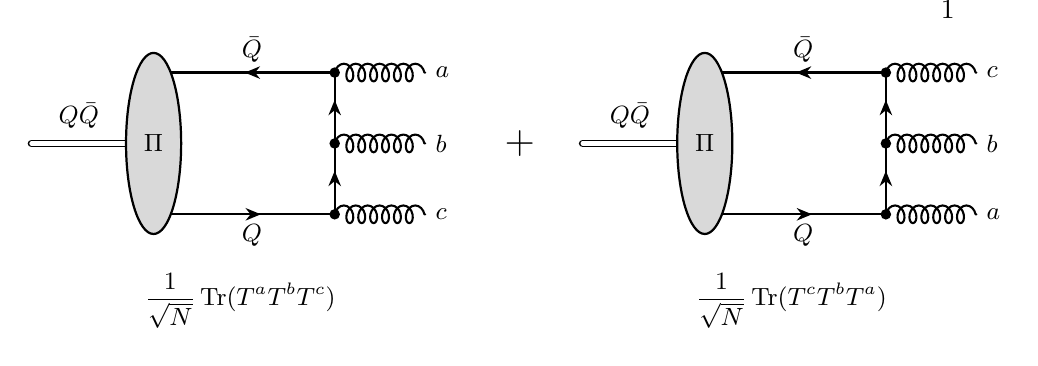
\begin{tikzpicture}[fd]
  % #1: xshift; #2,#3,#4: gluon labels top, middle, bottom; #5: colour factor
  \def\fdOnium#1#2#3#4#5{%
    \begin{scope}[xshift=#1]
      \draw[bound state] (-1.55,0) -- (-0.35,0);
      \node[above] at (-0.95,0.06) {$Q\bar Q$};
      \draw[quark] (0.22,-0.9) -- (2.3,-0.9);
      \draw[quark] (2.3,-0.9) -- (2.3,0);
      \draw[quark] (2.3,0) -- (2.3,0.9);
      \draw[quark] (2.3,0.9) -- (0.22,0.9);
      \draw[blob] (0,0) ellipse[x radius=0.35cm,y radius=1.15cm];
      \node at (0,0) {$\Pi$};
      \node[below] at (1.25,-0.9) {$Q$};
      \node[above] at (1.25,0.9) {$\bar Q$};
      \draw[gluon] (2.3,0.9) -- (3.45,0.9) node[right]{$#2$};
      \draw[gluon] (2.3,0) -- (3.45,0) node[right]{$#3$};
      \draw[gluon] (2.3,-0.9) -- (3.45,-0.9) node[right]{$#4$};
      \foreach \yy in {0.9,0,-0.9} \node[vertex] at (2.3,\yy) {};
      \node at (1.1,-2.0) {#5};
    \end{scope}}
  \fdOnium{0cm}{a}{b}{c}{$\dfrac{1}{\sqrt N}\Tr(T^aT^bT^c)$}
  \node[font=\Large] at (4.65,0) {$+$};
  \fdOnium{7.0cm}{c}{b}{a}{$\dfrac{1}{\sqrt N}\Tr(T^cT^bT^a)$}
\end{tikzpicture}
\caption{重夸克偶素 $Q\bar Q$ 湮灭为三个胶子（\cref{prop:app-quarkonium}）。灰色块 $\Pi$ 表示自旋投影 $\Pi_\Gamma$ 与色单态投影 $\delta_{ij}/\sqrt N$，后者把开放的夸克线闭合成一个色迹；
两图中胶子沿夸克线的发射次序互为反序（$\sigma$ 与 $\sigma^{\mathrm R}$），色因子逆着费米子箭头读出。
对 C~宇称为 $\eta_\Gamma=-1$ 的 ${}^3S_1$ 态（如 $J/\psi$），两图的 Dirac 部分相等，两图之和的色结构为 $\Tr(T^aT^bT^c)+\Tr(T^cT^bT^a)=\tfrac12 d^{abc}$。}
\label{fig:quarkonium}
\end{figure}

\begin{proposition}[重夸克偶素湮灭为胶子：最低阶的 C~选择定则]\label{prop:app-quarkonium}
沿用上面的记号，对 $\sigma\in S_n$ 令
\begin{equation}\label{eq:app-onium-A}
A_\Gamma(\sigma)=\TrD\Bigl[\gamma^{\mu_{\sigma(n)}}S\bigl(\tfrac P2-q^\sigma_{\le n-1}\bigr)\gamma^{\mu_{\sigma(n-1)}}\cdots\gamma^{\mu_{\sigma(2)}}S\bigl(\tfrac P2-q^\sigma_{\le1}\bigr)\gamma^{\mu_{\sigma(1)}}\,\Pi_\Gamma\Bigr],
\end{equation}
则在 $g^n$ 阶，$n$ 个胶子都直接从夸克线发射的全部图之和（经自旋与色单态投影）为
\begin{equation}\label{eq:app-onium-amp}
\mathcal A_n=\frac{(\ii g)^n}{\sqrt N}\sum_{\sigma\in S_n}\tau_\sigma\,A_\Gamma(\sigma),\qquad \tau_\sigma:=\Tr\bigl(T^{a_{\sigma(n)}}\cdots T^{a_{\sigma(1)}}\bigr),
\end{equation}
并且：
\begin{enumerate}[label=(\roman*),leftmargin=2em,itemsep=1pt,topsep=2pt]
\item $\Cconj{\Pi_\Gamma}=\eta_\Gamma\Pi_\Gamma$，其中 $\eta_{\gamma^5}=+1$，$\eta_{\sla\varepsilon}=-1$；这对任意 $P$ 与 $\varepsilon$ 成立（不需要 $P^2=4m^2$ 或 $\varepsilon\cdot P=0$）。
\item 记 $\sigma^{\mathrm R}(i):=\sigma(n+1-i)$（发射次序反转），则 $A_\Gamma(\sigma^{\mathrm R})=\eta_\Gamma(-1)^n A_\Gamma(\sigma)$。
\item $\mathcal A_n=\frac{(\ii g)^n}{\sqrt N}\sum_{\sigma\in S_n}\bigl(\mathcal P_{\eta_\Gamma}\tau_\sigma\bigr)A_\Gamma(\sigma)$：每个色迹中只有 C~宇称为 $\eta_\Gamma$ 的部分存活。
\item 特别地，对 ${}^3S_1$（$\Gamma=\sla\varepsilon$，如 $J/\psi$）：$\mathcal A_2\equiv0$（对一切离壳的 $q_1+q_2=P$ 与一切 $\mu_1,\mu_2$），且
$\mathcal A_3=\frac{(\ii g)^3}{4\sqrt N}\,d^{a_1a_2a_3}\sum_{\sigma\in S_3}A_\Gamma(\sigma)$；
对 ${}^1S_0$（$\Gamma=\gamma^5$，如 $\eta_c$）：$\mathcal A_2=\frac{(\ii g)^2}{\sqrt N}\,\delta^{a_1a_2}A_\Gamma(\mathrm{id})$，且
$\mathcal A_3=-\frac{g^3}{4\sqrt N}\,f^{a_1a_2a_3}\sum_{\sigma\in S_3}\operatorname{sgn}(\sigma)A_\Gamma(\sigma)$。
\end{enumerate}
\end{proposition}

\begin{proof}
\cref{eq:app-onium-amp}只是把顶点因子 $\ii g\gamma^\mu T^a$、传播子与两个投影按上述次序代入的结果。

\emph{(i)} 由 Clifford 共轭的反自同构性质（\cref{lem:C-matrix}）与 $\Cconj{\sla P}=-\sla P$，
\begin{equation*}
\Cconj{\Pi_\Gamma}=\Cconj{\bigl(\tfrac12\sla P-m\bigr)}\,\Cconj\Gamma\,\Cconj{\bigl(\tfrac12\sla P+m\bigr)}=\bigl(-\tfrac12\sla P-m\bigr)\,\eta_\Gamma\Gamma\,\bigl(-\tfrac12\sla P+m\bigr)=\eta_\Gamma\,\Pi_\Gamma ,
\end{equation*}
其中由\cref{lem:C-parity}，$\eta_{\gamma^5}=+1$，$\eta_{\sla\varepsilon}=\eta_{\gamma^\mu}=-1$（Clifford 共轭是线性的，复系数 $\varepsilon_\mu$ 不受影响）。

\emph{(ii)} 记\cref{eq:app-onium-A}中迹内的矩阵为 $X$，$k_j:=\frac P2-q^\sigma_{\le j}$。由 $\TrD X=\TrD\Cconj X$、反自同构性质、(i)、$\Cconj{\gamma^\mu}=-\gamma^\mu$ 与\cref{lem:propagator}，
\begin{equation*}
A_\Gamma(\sigma)=\TrD\Cconj X=\eta_\Gamma(-1)^n\,\TrD\Bigl[\Pi_\Gamma\,\gamma^{\mu_{\sigma(1)}}S(-k_1)\gamma^{\mu_{\sigma(2)}}S(-k_2)\cdots S(-k_{n-1})\gamma^{\mu_{\sigma(n)}}\Bigr].
\end{equation*}
由 $\sum_iq_i=P$，$-k_j=q^\sigma_{\le j}-\frac P2=\frac P2-\sum_{i>j}q_{\sigma(i)}=\frac P2-q^{\sigma^{\mathrm R}}_{\le n-j}$，又 $\sigma(j)=\sigma^{\mathrm R}(n+1-j)$。
把 $\Pi_\Gamma$ 循环移到最右边，右边的迹恰为 $A_\Gamma(\sigma^{\mathrm R})$，故 $A_\Gamma(\sigma)=\eta_\Gamma(-1)^nA_\Gamma(\sigma^{\mathrm R})$，与所述等价（$\eta_\Gamma^2=1$）。
这里用到了 $\sum_jq_j=P$ 以及夸克与反夸克的动量相等（都为 $P/2$），没有用到 $P^2=4m^2$、$\varepsilon\cdot P=0$ 或胶子在壳；若破坏 $\sum_jq_j=P$，恒等式一般不成立（我们也作了这一数值检验）。

\emph{(iii)} $n=1$ 时 $\tau_\sigma=\Tr T^{a_1}=0$，两边都为零。设 $n\ge2$，则 $\sigma^{\mathrm R}\neq\sigma$，$S_n$ 分解为不相交的二元组 $\{\sigma,\sigma^{\mathrm R}\}$。
$\tau_{\sigma^{\mathrm R}}=\Tr(T^{a_{\sigma(1)}}\cdots T^{a_{\sigma(n)}})$ 是 $\tau_\sigma$ 的反序迹，由\cref{eq:color-reversal}，$(-1)^n\tau_{\sigma^{\mathrm R}}=\Rop\tau_\sigma$。于是由 (ii)，
\begin{equation}\label{eq:app-onium-pair}
\tau_\sigma A_\Gamma(\sigma)+\tau_{\sigma^{\mathrm R}}A_\Gamma(\sigma^{\mathrm R})=\bigl(\tau_\sigma+\eta_\Gamma\Rop\tau_\sigma\bigr)A_\Gamma(\sigma)=2\bigl(\mathcal P_{\eta_\Gamma}\tau_\sigma\bigr)A_\Gamma(\sigma).
\end{equation}
又 $\mathcal P_\eta\Rop=\frac12(\Rop+\eta)=\eta\,\mathcal P_\eta$，故 $(\mathcal P_{\eta_\Gamma}\tau_{\sigma^{\mathrm R}})A_\Gamma(\sigma^{\mathrm R})=\eta_\Gamma(\mathcal P_{\eta_\Gamma}\Rop\tau_\sigma)A_\Gamma(\sigma)=(\mathcal P_{\eta_\Gamma}\tau_\sigma)A_\Gamma(\sigma)$，
即\cref{eq:app-onium-pair}右边也等于 $(\mathcal P_{\eta_\Gamma}\tau_\sigma)A_\Gamma(\sigma)+(\mathcal P_{\eta_\Gamma}\tau_{\sigma^{\mathrm R}})A_\Gamma(\sigma^{\mathrm R})$。对全部二元组求和即得 (iii)。

\emph{(iv)} $n=2$：$\tau_\sigma=\frac12\delta^{a_1a_2}$ 是 C~偶的（\cref{lem:R-properties}(iii)），故 $\Pm\tau_\sigma=0$，$\Pp\tau_\sigma=\tau_\sigma$。对 $\eta_\Gamma=-1$ 由 (iii) 得 $\mathcal A_2=0$；
对 $\eta_\Gamma=+1$，由 (ii) 有 $A_\Gamma(21)=A_\Gamma(12)$，代入 (iii) 得所述结果。$n=3$：由\cref{eq:trace3}，$\Pm\tau_\sigma=\frac14d^{a_{\sigma(3)}a_{\sigma(2)}a_{\sigma(1)}}=\frac14d^{a_1a_2a_3}$（$d^{abc}$ 全对称），
$\Pp\tau_\sigma=\frac{\ii}{4}f^{a_{\sigma(3)}a_{\sigma(2)}a_{\sigma(1)}}=-\frac{\ii}{4}\operatorname{sgn}(\sigma)f^{a_1a_2a_3}$（$f^{abc}$ 全反对称，而 $i\mapsto\sigma(4-i)$ 的符号为 $-\operatorname{sgn}\sigma$）。
代入 (iii) 并用 $(\ii g)^3\cdot(-\frac{\ii}{4})=-\frac{g^3}{4}$ 即得两个 $\mathcal A_3$ 的表达式。
\end{proof}

\begin{remark}[色因子 $5/18$]\label{rem:app-onium-colour}
由 (iv) 与 $d^{abc}d^{abc}=(N^2-4)(N^2-1)/N$（\cref{lem:app-traces-contractions}），${}^3S_1$ 态的
\begin{equation}\label{eq:app-onium-colour}
\sum_{a_1,a_2,a_3}\bigl|\mathcal A_3\bigr|^2=g^6\,\frac{(N^2-4)(N^2-1)}{16N^2}\,\Bigl|\sum_{\sigma\in S_3}A_\Gamma(\sigma)\Bigr|^2,\qquad \frac{(N^2-4)(N^2-1)}{16N^2}\Big|_{N=3}=\frac{5}{18}.
\end{equation}
若把三个胶子换成三个光子（夸克电荷 $e_Q$，顶点 $-\ii ee_Q\gamma^\mu\otimes\mathbb 1$，\cref{cor:qed}），色单态投影给出 $\frac1{\sqrt N}\Tr\mathbb 1_N=\sqrt N$，振幅为 $(-\ii ee_Q)^3\sqrt N\sum_\sigma A_\Gamma(\sigma)$，色因子为 $N$。
两种情形的 Dirac 部分是同一个 Abel 型的和 $\sum_{\sigma}A_\Gamma(\sigma)$；对质壳上的 $\Pi_\Gamma$，它满足与 QED 相同的 Ward 恒等式，故极化求和与相空间也相同。
（对胶子，这一阶含三胶子或四胶子顶点的图对 ${}^3S_1$ 都为零：其夸克线部分或为 $Q\bar Q\to gg^*$，而 $\mathcal A_2\equiv0$；或为 $Q\bar Q\to g^*$，而 $\mathcal A_1\propto\Tr T^a=0$。）于是在最低阶
$\varGamma({}^3S_1\to ggg)/\varGamma({}^3S_1\to\gamma\gamma\gamma)=(g/ee_Q)^6\,(N^2-4)(N^2-1)/(16N^3)=\frac{5}{54}\bigl(\alpha_s/e_Q^2\alpha\bigr)^3$（$N=3$）；
与色因子为 $1$ 的正电子偶素三光子湮灭\cite{OrePowell1949}相比（取相同的质量、波函数与 Dirac 结构），比值为 $\frac{5}{18}(\alpha_s/\alpha)^3$。这一类比是把 $J/\psi$ 的强衰变归于三胶子过程的出发点\cite{AppelquistPolitzer1975PRL,AppelquistPolitzer1975PRD}（综述见\cite{Novikov1978}；$d^{abc}$ 色结构及其色因子亦见\cite{Jia2007}）。
\end{remark}

\begin{remark}[C~与 Landau--Yang 定理的分工]\label{rem:app-onium-LY}
(a) $J/\psi\to gg$ 被 C~禁戒：(iv) 对任意离壳胶子给出 $\mathcal A_2\equiv0$；同阶的另一个图 $Q\bar Q\to g^*\to gg$（经三胶子顶点）的夸克线部分为 $\mathcal A_1\propto\Tr T^a=0$，
它为零是由于色而不是 C，所以 $g^2$ 阶（最低阶）的整个振幅对任意离壳胶子都为零。对在壳胶子，$J/\psi\to gg$ 同时被 Landau--Yang 定理禁戒\cite{Landau1948,Yang1950}：自旋为 $1$ 的粒子不能衰变为两个光子。
其证明只用到末态是两个全同的在壳无质量矢量粒子、且末态在二者交换下对称（Bose 对称性），因而同样适用于色单态的双胶子态：其色波函数 $\delta^{ab}$ 是对称的，剩余的自旋--轨道波函数在交换下必须像两个光子那样对称。
(b) $\chi_{c1}$（${}^3P_1$，$J^{PC}=1^{++}$）的 C~宇称为 $+1$，C~允许色对称的 $\delta^{ab}$ 双胶子态；$\chi_{c1}\to gg$（在壳）之所以被禁戒，是由于 Landau--Yang 定理而不是 C。
(c) $\eta_c\to gg$ 为 C~所允许（$\propto\delta^{ab}$）；$\eta_c\to ggg$ 的夸克线部分 $\propto f^{abc}$。$J/\psi\to ggg$ 为 C~所允许，三胶子处于 C~奇的 $d^{abc}$ 型色单态（\cref{sec:applications-glue}）。
$J/\psi\to\gamma gg$ 中光子顶点与投影的 C~宇称之积为 $(-1)(-1)=+1$，双胶子处于 $\delta^{ab}$ 态，为 C~所允许；$J/\psi\to\gamma\gamma$ 则被 C（$(-1)^3=-1$）与 Landau--Yang 定理同时禁戒。这些归类与\cref{tab:thmI-examples}一致。
\end{remark}

\begin{remark}[非静态推广与任意阶]\label{rem:app-onium-allorders}
(a) 若夸克与反夸克的动量为 $p=\frac P2+r$、$\bar p=\frac P2-r$，投影 $\Pi_\Gamma(r)=(\sla p+m)\Gamma(\sla{\bar p}-m)$ 满足 $\Cconj{\Pi_\Gamma(r)}=\eta_\Gamma\Pi_\Gamma(-r)$（与 (i) 的计算相同），
(ii) 的证明给出发射次序反转同时伴随 $r\mapsto-r$。对相对动量作分波投影后，$r\mapsto-r$ 提供因子 $(-1)^L$，于是有效的 C~宇称为 $(-1)^{L+S}$。
(b) 在更高阶，经投影的振幅还包含胶子自相互作用、圈修正以及夸克线与其余部分之间的胶子交换。在带标号的展开中，开放夸克线连同 $\Pi_\Gamma$ 与色单态投影构成一条“闭合”的链 $\Tr[\Pi_\Gamma\,\mathsf O]$，
$\mathsf O$ 是从 $Q$ 端到 $\bar Q$ 端的开放夸克线（逆着箭头写出的矩阵之积）。把\cref{def:rho}中的 $\rho$ 推广为把这条链与全部闭合夸克圈同时反向。对这条链，\cref{rem:thmI-open-lines}的开放线反向恒等式与 (i) 给出与\cref{lem:thmII-rho-value}相同的关系，只多一个因子 $\eta_\Gamma$。
开放线上还可以有 (V1) 型抵消项顶点与 (V3) 型两点插入：前者与普通顶点相同，后者按\cref{rem:thmI-derivative}处理。在动量空间中开放线取镜像配置（同\cref{lem:thmII-rho-value}证明的第三、四步）；
由于两端的动量都是 $P/2$，反向后的动量配置仍属同一类（(ii) 的证明正是其最低阶情形）。由此在\cref{thm:furry-allorders}的假设下，经投影的振幅满足 $\Rop\mathcal A=\eta_\Gamma\mathcal A$：
色单态投影起 C~宇称为 $\eta_\Gamma=(-1)^S$ 的色单态插入的作用（$L\neq0$ 时结合 (a)，C~宇称为 $(-1)^{L+S}$）。再结合整体 $\mathrm{SU}(N)$ 不变性与\cref{lem:invariants}（论证同\cref{cor:selection}(b)），${}^3S_1\to gg$ 在 $\alpha_s$ 的任意阶为零，
${}^3S_1\to ggg$ 只含 $d^{abc}$，${}^1S_0\to ggg$ 只含 $f^{abc}$。以上是论证的要点；其余细节与\cref{thm:furry-allorders}的证明相同（以\cref{rem:thmI-open-lines}代替闭合圈的反向恒等式），本文不再重复。
\end{remark}

%% ----------------------------------------------------------------------
\subsection{夸克圈色序振幅的反射恒等式}\label{sec:applications-reflection}

设 $n\ge2$ 个外胶子 $(p_j,\mu_j,a_j)$，动量全部流入，$\sum_jp_j=0$。考虑截腿的单圈 $n$ 胶子 Green 函数（动量空间，略去整体因子 $(2\pi)^D\delta(\sum_jp_j)$）中，
$n$ 个外胶子都直接连在同一个味道的夸克圈上的那部分，记为 $\Gamma^{(q)}$；也就是说，夸克圈恰有 $n$ 个夸克--胶子顶点，每个顶点的胶子线都是外线。
对满足 $\sigma(1)=1$ 的 $\sigma\in S_n$（它们是循环次序 $S_n/\mathbb Z_n$ 的代表元）定义
\begin{equation}\label{eq:app-refl-A}
\begin{gathered}
A^q(\sigma)=-(\ii g)^n\!\int\!\frac{\dd^Dk}{(2\pi)^D}\,\TrD\bigl[\gamma^{\mu_{\sigma(1)}}S(k_1)\gamma^{\mu_{\sigma(2)}}S(k_2)\cdots\gamma^{\mu_{\sigma(n)}}S(k_n)\bigr],\\
k_n=k,\qquad k_{j-1}=k_j+p_{\sigma(j)}\quad(j=n,n-1,\dots,2),
\end{gathered}
\end{equation}
即 $k_j$ 是从顶点 $\sigma(j+1)$ 流向顶点 $\sigma(j)$ 的夸克线动量（$k_0\equiv k_n$ 由 $\sum_jp_j=0$ 保证），与\cref{def:loop-factor}的逆箭头次序一致；这就是\cref{eq:dirac-polygon}的多边形配置（$p_j\to p_{\sigma(j)}$）。
注意本小节的 $\tau_\sigma$ 与 $\sigma^{\mathrm R}$ 按循环次序定义（\cref{prop:app-reflection}），与\cref{sec:applications-quarkonium}中开放夸克线的同名记号不同。

\begin{proposition}[夸克圈色序振幅的反射恒等式]\label{prop:app-reflection}
在维数正规化（或任何满足\cref{def:reg-hypotheses}中的 (R1)、且圈积分在积分变量的平移与反射下都不变的正规化，例如作用于夸克线的 Pauli--Villars 正规化）中，
\begin{equation}\label{eq:app-refl-decomp}
\Gamma^{(q)}=\sum_{\substack{\sigma\in S_n\\ \sigma(1)=1}}\Tr\bigl(T^{a_{\sigma(1)}}T^{a_{\sigma(2)}}\cdots T^{a_{\sigma(n)}}\bigr)\,A^q(\sigma);
\end{equation}
并且对 $\sigma(1)=1$ 的 $\sigma$，令 $\sigma^{\mathrm R}:=(\sigma(1),\sigma(n),\sigma(n-1),\dots,\sigma(2))$（反向的循环次序），有
\begin{equation}\label{eq:app-refl}
A^q(\sigma^{\mathrm R})=(-1)^n\,A^q(\sigma).
\end{equation}
因此当 $n\ge3$ 时，$\Gamma^{(q)}=\sum_{\{\sigma,\sigma^{\mathrm R}\}}2\bigl(\Pp\tau_\sigma\bigr)A^q(\sigma)$，求和遍及反射对，$\tau_\sigma=\Tr(T^{a_{\sigma(1)}}\cdots T^{a_{\sigma(n)}})$，
$2\Pp\tau_\sigma$ 在 $n$ 为偶数时为 $2\Real\tau_\sigma$，在 $n$ 为奇数时为 $2\ii\Imag\tau_\sigma$。
\end{proposition}

\begin{proof}
\emph{第一步（色分解）。}在带标号的展开中（\cref{sec:setup-expansion}），对 $\Gamma^{(q)}$ 有贡献的缩并含 $n$ 个夸克--胶子顶点 $z_1,\dots,z_n$，夸克置换是一个 $n$ 循环 $\ell=(i_1\cdots i_n)$，
胶子配对 $P$ 把 $n$ 个顶点胶子槽位与 $n$ 个外胶子场一一配对，记相应的双射为 $\beta$（顶点 $\mapsto$ 外胶子）。由\cref{lem:closed-loops}与\cref{eq:loop-factorized}，
这样的缩并给出 $-(\ii g)^n\,\Tr(T^{a_{\beta(i_1)}}\cdots T^{a_{\beta(i_n)}})$ 乘以 Dirac 迹（顶点上的色指标经胶子传播子的 $\delta$ 与外指标缩并）。
它只依赖于外胶子沿圈（逆着箭头）的循环次序 $(\beta(i_1),\dots,\beta(i_n))$：对给定的循环次序，产生它的 $(\ell,\beta)$ 恰有 $n!$ 个（任取 $\beta$，则 $\ell$ 被唯一确定），
它们对顶点位置积分后的值相同（只是积分变量的重新命名），这 $n!$ 正好抵消\cref{eq:setup-Nnu}中的 $1/n!$。截去外胶子传播子并作 Fourier 变换，圈积分按\cref{eq:app-refl-A}的动量配置给出 $A^q(\sigma)$（圈积分在平移下不变，故圈动量的选取不影响结果），即得\cref{eq:app-refl-decomp}。

\emph{第二步（反射）。}对被积函数用\cref{eq:loop-reversal-mom}（$\Gamma_j=\gamma^{\mu_{\sigma(j)}}$，$\eta_j=-1$，$q_j=k_j$）：
\begin{equation*}
\TrD\bigl[\gamma^{\mu_{\sigma(1)}}S(k_1)\cdots\gamma^{\mu_{\sigma(n)}}S(k_n)\bigr]=(-1)^n\,\TrD\bigl[\gamma^{\mu_{\sigma(1)}}S(-k_n)\gamma^{\mu_{\sigma(n)}}S(-k_{n-1})\cdots\gamma^{\mu_{\sigma(2)}}S(-k_1)\bigr].
\end{equation*}
右边正是 $A^q(\sigma^{\mathrm R})$ 的被积函数在圈动量 $k':=-k_1=p_{\sigma(1)}-k$ 处的值：对 $\sigma^{\mathrm R}$，$k'_n=k'$，$k'_{j-1}=k'_j+p_{\sigma^{\mathrm R}(j)}$，而 $\sigma^{\mathrm R}(j)=\sigma(n+2-j)$（$j\ge2$），由归纳法
\begin{gather*}
k'_j=-k_{n+1-j}\quad\bigl(k'_{j-1}=-k_{n+1-j}+p_{\sigma(n+2-j)}=-k_{n+2-j}\bigr);\\
k_1=k_n+\textstyle\sum_{j\ge2}p_{\sigma(j)}=k-p_{\sigma(1)}.
\end{gather*}
这就是 $\sigma^{\mathrm R}$ 的镜像动量配置（\cref{fig:dirac-mirror}）。对 $k$ 积分，变换 $k\mapsto p_{\sigma(1)}-k$（平移加反射）保持圈积分（维数正规化中即\cref{prop:reg-dimreg}证明中的 (I2) 与 (I3)；绝对收敛的 Pauli--Villars 积分亦然），故得\cref{eq:app-refl}（平移与反射不变性在此不可省去，见\cref{rem:app-refl-cutoff}）。

\emph{第三步（反射对的色因子）。}当 $n\ge3$ 时 $\sigma^{\mathrm R}(2)=\sigma(n)\neq\sigma(2)$，故 $\sigma^{\mathrm R}\neq\sigma$。由迹的循环性，$\tau_{\sigma^{\mathrm R}}$ 是 $\tau_\sigma$ 的反序迹：
\begin{equation*}
\begin{gathered}
\tau_{\sigma^{\mathrm R}}=\Tr\bigl(T^{a_{\sigma(1)}}T^{a_{\sigma(n)}}\cdots T^{a_{\sigma(2)}}\bigr)=\Tr\bigl(T^{a_{\sigma(n)}}\cdots T^{a_{\sigma(2)}}T^{a_{\sigma(1)}}\bigr),\\
\tau_\sigma A^q(\sigma)+\tau_{\sigma^{\mathrm R}}A^q(\sigma^{\mathrm R})=\bigl[\tau_\sigma+(-1)^n\tau_{\sigma^{\mathrm R}}\bigr]A^q(\sigma)=2\bigl(\Pp\tau_\sigma\bigr)A^q(\sigma),
\end{gathered}
\end{equation*}
其中第二行用了\cref{eq:app-refl}与\cref{eq:bracket}。
（$n=2$ 时 $\sigma^{\mathrm R}=\sigma$，\cref{eq:app-refl}只是平凡的等式，与长度不超过 $2$ 的圈自反向一致，参见\cref{rem:thmI-short-loops}。）
\end{proof}

\begin{remark}[截断正规化下的反射恒等式]\label{rem:app-refl-cutoff}
朴素截断只以 (R2) 的第二种形式满足\cref{def:reg-hypotheses}（\cref{tab:reg-schemes}）；按\cref{eq:app-refl-A}，$A^q(\sigma^{\mathrm R})$ 是对其自身的圈动量 $k'$ 截断的，而 $\sigma$ 的镜像配置要求对 $k=p_{\sigma(1)}-k'$ 截断；
球形截断在反射下不变，但这里的平移产生\cref{sec:reg-cutoff}中的表面项，故\cref{eq:app-refl}一般不成立。例如 $n=3$、$\sigma=(1,2,3)$ 时（外胶子 $1,2,3$ 为 $(a,\mu,p_1)$、$(b,\nu,p_2)$、$(c,\rho,p_3)$），
$A^q(\sigma^{\mathrm R})$ 的 Dirac 迹正是\cref{rem:tri-cutoff}中的 $F_B^{\mathrm{can}}$（$A^q(\sigma)$ 的则是 $F_A$），由\cref{eq:tri-surface}与\cref{eq:tri-DeltaA}，Euclid 球形截断下
$A^q(\sigma)+A^q(\sigma^{\mathrm R})\to(\ii g)^3\Delta_A(p_1)=\frac{\ii g^3}{24\pi^2}\mathcal S^{\mu\nu\rho}(p_1)\neq0$（$\Lambda\to\infty$，$\mathcal S$ 见\cref{eq:tri-Sdef}）。
在这类正规化中，应对每个反射对取定代表元 $\sigma$ 按\cref{eq:app-refl-A}配置，而把 $A^q(\sigma^{\mathrm R})$ 按 $\sigma$ 的镜像配置计算（在其被积函数中令圈动量为 $p_{\sigma(1)}-k$，并对 $k$ 施加与 $A^q(\sigma)$ 相同的截断），
$\Gamma^{(q)}$ 中的缩并也按同一配置计算；这样\cref{eq:app-refl-decomp}与\cref{eq:app-refl}仍成立，后者由证明第二步中的逐点恒等式直接得到。
\end{remark}

\begin{remark}[与前文的一致性]\label{rem:app-refl-consistency}
$n=3$ 时，取 $(a,\mu,p_1)$、$(b,\nu,p_2)$、$(c,\rho,p_3)$ 为外胶子 $1,2,3$：$k_3=k$，$k_2=k+p_3$，$k_1=k-p_1$，故 $A^q(1,2,3)=-(\ii g)^3I^{\mu\nu\rho}$（$I$ 见\cref{prop:triangle}），而
$\Gamma^{(q)}=\bigl[\Tr(T^aT^bT^c)-\Tr(T^aT^cT^b)\bigr]A^q(1,2,3)=\frac{\ii}{2}f^{abc}\cdot\ii g^3I^{\mu\nu\rho}=-\frac{g^3}{2}f^{abc}I^{\mu\nu\rho}$，与\cref{prop:triangle}(i) 一致。
$n=4$ 时六个循环次序组成三个反射对，每对给出 $2\Real\Tr$，与\cref{fig:boxes}一致。
\end{remark}

\begin{remark}[完整的偏振幅与文献]\label{rem:app-refl-full}
单圈夸克贡献中还有胶子树连在夸克圈上的图。反复使用恒等式 $f^{xbc}T^x=-\ii[T^b,T^c]$（及其对四胶子顶点的推论），每个这样的图的色因子都化为单迹 $\tau_\sigma$ 的组合，且系数与 $N$ 无关
（单圈时没有内胶子线连接夸克圈上的两点，因而不出现 Fierz 恒等式中的 $1/N$ 项）。于是完整的单圈夸克贡献可写成 $\sum_{\sigma(1)=1}\tau_\sigma A^q_{\mathrm{full}}(\sigma)$，$A^q_{\mathrm{full}}$ 与 $N$ 无关。
单圈、只含外胶子的缩并集合在 $\rho$ 下封闭，由\cref{thm:furry-allorders}，$\Rop\Gamma^{(q)}_{\mathrm{full}}=\Gamma^{(q)}_{\mathrm{full}}$；再由 $(-1)^n\tau_{\sigma^{\mathrm R}}=\Rop\tau_\sigma$ 得
\begin{equation*}
\sum_{\sigma(1)=1}\tau_\sigma\Bigl[A^q_{\mathrm{full}}(\sigma)-(-1)^nA^q_{\mathrm{full}}(\sigma^{\mathrm R})\Bigr]=0 .
\end{equation*}
$N\ge n$ 时这些单迹线性无关（\cref{lem:invariants}的证明第二步），而系数与 $N$ 无关，
故\cref{eq:app-refl}对完整的偏振幅 $A^q_{\mathrm{full}}$ 同样成立（在壳时它们是规范不变的；正规化的条件与\cref{prop:app-reflection}相同）。对纯 $\mathrm{SU}(N)$ 规范理论，树图色序振幅的反射恒等式见\cite{BernKosower1991,ManganoParke1991}，Bern 与 Kosower 还对胶子圈导出了单圈色序振幅的反射恒等式\cite{BernKosower1991}；
色分解的一般讨论见\cite{ManganoParke1991,Dixon1996TASI}。文献中的归一化不尽相同（例如\cite{Dixon1996TASI}取 $\Tr(T^aT^b)=\delta^{ab}$，$[T^a,T^b]=\ii\sqrt2f^{abc}T^c$），
但改变归一化 $T^a\to\lambda T^a$（同时 $g\to g/\lambda$）不改变 $\Gamma^{(q)}$，只把每个偏振幅 $A^q(\sigma)$（及 $A^q_{\mathrm{full}}(\sigma)$）乘以同一个因子 $\lambda^{-n}$，
故\cref{eq:app-refl}不受影响。
\end{remark}

%% ----------------------------------------------------------------------
\subsection{胶子态的 C~宇称、胶球与奇子}\label{sec:applications-glue}

\paragraph{色单态胶子态。}由\cref{eq:np-gluon-states}，色波函数为 $t$ 的多胶子态满足 $\Cop|t\rangle=|\Rop t\rangle$，其余量子数不变；色单态对应于不变张量 $t\in\mathrm{Inv}_n$，
其 C~宇称就是 $t$ 的 C~宇称。由\cref{lem:invariants}：两个胶子的色单态只有 $\delta^{ab}$，总是 C~偶的；三个胶子有 $f^{abc}$（C~偶）与 $d^{abc}$（C~奇，$N\ge3$）两种色单态\cite{Ewerz2003}；
$N=2$ 时一切色单态都是 C~偶的（\cref{prop:su2}）。一般地，由\cref{eq:color-TT}，每个色迹都是 $\delta^{ab}$、$f^{abc}$、$d^{abc}$ 的缩并多项式，而 $\mathrm{Inv}_n$ 由色迹之积张成（\cref{lem:invariants}的证明第二步），
所以每个不变张量都是 $\delta^{ab}$、$f^{abc}$、$d^{abc}$ 的单项式之和；含 $k$ 个 $d^{abc}$ 型因子的单项式的 C~宇称为 $(-1)^k$（\cref{lem:R-properties}(iii) 与\cref{lem:contraction}(i)）。
因此 C~奇的色单态胶子态的色波函数是含奇数个 $d^{abc}$ 型因子的单项式之和，在三胶子中 $d^{abc}$ 是唯一的（相差归一化）C~奇色单态。

\paragraph{规范不变的胶子算符。}设 $X_k$ 是按伴随表示协变的场（$F_{\mu\nu}$、$\tilde F_{\mu\nu}$、$D_\rho F_{\mu\nu}$ 等），由\cref{eq:np-F}及同样的计算，$X_k\mapsto-X_k^{\tp}$。于是
$\Tr(X_1X_2)\mapsto\Tr(X_1^{\tp}X_2^{\tp})=\Tr(X_1X_2)$ 总是 C~偶的，而 $\Tr(X_1X_2X_3)\mapsto-\Tr(X_1^{\tp}X_2^{\tp}X_3^{\tp})=-\Tr(X_3X_2X_1)$。由\cref{eq:color-fd-traces}，
\begin{equation}\label{eq:app-glue-ops}
\begin{gathered}
\Tr\bigl(X_1\{X_2,X_3\}\bigr)=\tfrac12d^{abc}X_1^aX_2^bX_3^c\quad(\text{C~奇}),\\
\Tr\bigl(X_1[X_2,X_3]\bigr)=\tfrac{\ii}{2}f^{abc}X_1^aX_2^bX_3^c\quad(\text{C~偶}),
\end{gathered}
\end{equation}
所以 C~奇的纯胶子算符至少含三个伴随协变场 $X_k$；恰含三个时，色结构必为 $d^{abc}$（一般地，其色张量是含奇数个 $d^{abc}$ 型因子的单项式之和）。需要注意，Lorentz 指标完全循环缩并的 $Y^{abc}:=F^{a\mu}{}_\nu F^{b\nu}{}_\rho F^{c\rho}{}_\mu$ 是 Lorentz 矩阵之积的迹，
因而在 $(abc)$ 的循环置换下不变；而把迹转置并用 $F_{\mu\nu}=-F_{\nu\mu}$，每个因子贡献一个负号，得 $Y^{cba}=(-1)^3Y^{abc}$。所以 $Y^{abc}$ 全反对称，
\begin{equation}\label{eq:app-glue-vanish}
d^{abc}F^{a\mu}{}_\nu F^{b\nu}{}_\rho F^{c\rho}{}_\mu\equiv0 ,
\end{equation}
存活的只是 C~偶的 $f^{abc}F^{a\mu}{}_\nu F^{b\nu}{}_\rho F^{c\rho}{}_\mu$。一个不为零的 C~奇算符是
\begin{equation}\label{eq:app-glue-Od}
O_d^{\rho\sigma}:=d^{abc}F^a_{\mu\nu}F^{b\mu\nu}F^{c\rho\sigma}=4\Tr\bigl(F^{\rho\sigma}F_{\mu\nu}F^{\mu\nu}\bigr)
\end{equation}
（第二个等号用\cref{eq:trace3}及 $F^a_{\mu\nu}F^{b\mu\nu}$ 关于 $a,b$ 的对称性；由 $\Tr(X_1X_2X_3)\mapsto-\Tr(X_3X_2X_1)$ 与迹的循环性可知它是 C~奇的）。它不恒为零：取 $F^a_{\mu\nu}=n^a\omega_{\mu\nu}$，
则 $O_d^{\rho\sigma}=d^{abc}n^an^bn^c\,(\omega_{\mu\nu}\omega^{\mu\nu})\,\omega^{\rho\sigma}$，而 $N\ge3$ 时存在 $n$ 使 $d^{abc}n^an^bn^c=4\Tr(n^aT^a)^3\neq0$（\cref{eq:color-dxxx}）。\cref{eq:app-glue-vanish}与\cref{eq:app-glue-Od}都已数值核验。

\paragraph{胶球。}在格点上（\cref{thm:lattice}），C~偶与 C~奇的算符严格不混合（交叉关联函数为零），因此 C~奇胶球道可以用 $\Imag W_\gamma$ 型算符（\cref{tab:np-operators}，再按格点转动群投影到确定的 $J^{PC}$）单独研究。
$\mathrm{SU}(3)$ 的格点计算给出了包括若干 C~奇道在内的胶球谱\cite{MorningstarPeardon1999}。对 $\mathrm{SU}(2)$，C~奇的纯胶子扇区是空的（\cref{rem:np-su2}）。

\paragraph{奇子。}奇子（odderon）是高能弹性散射中与坡密子（pomeron）相对的 C~奇交换\cite{LukaszukNicolescu1973}，它对粒子--粒子与粒子--反粒子散射的贡献符号相反；综述见\cite{Ewerz2003}。
在微扰 QCD 中，最低阶的奇子是三个胶子处于 C~奇的 $d^{abc}$ 型色单态的交换，而 $f^{abc}$ 型三胶子态是 C~偶的\cite{Ewerz2003}。相应的色代数如下：由\cref{eq:app-traces-fTT}与 $T^aT^a=C_F\mathbb 1$，
\begin{equation}\label{eq:app-glue-odd}
d^{abc}T^aT^bT^c=\frac{N^2-4}{2N}\,C_F\,\mathbb 1,\qquad f^{abc}T^aT^bT^c=\frac{\ii N}{2}\,C_F\,\mathbb 1 ,
\end{equation}
且 $d^{abc}$ 型耦合与三个生成元的次序无关（$d^{abc}$ 全对称）。换成反夸克的生成元 $T^a_{\bar F}=-(T^a)^{\tp}$（\cref{lem:color-reversal}）时，
\begin{equation*}
\begin{gathered}
d^{abc}T^a_{\bar F}T^b_{\bar F}T^c_{\bar F}=-\bigl(d^{abc}T^cT^bT^a\bigr)^{\tp}=-\frac{N^2-4}{2N}\,C_F\,\mathbb 1,\\
f^{abc}T^a_{\bar F}T^b_{\bar F}T^c_{\bar F}=-\bigl(f^{abc}T^cT^bT^a\bigr)^{\tp}=+\frac{\ii N}{2}\,C_F\,\mathbb 1 .
\end{gathered}
\end{equation*}
所以 $d^{abc}$ 型三胶子色单态与夸克线的耦合在夸克与反夸克之间变号，$f^{abc}$ 型的不变号——这正是 $\Cop|t\rangle=|\Rop t\rangle$ 对 $t=d^{abc}$（$\Rop t=-t$）与 $t=f^{abc}$（$\Rop t=t$）在耦合上的体现。
$N=2$ 时 $d^{abc}\equiv0$，
不存在 C~奇的三胶子色单态交换。

%% ----------------------------------------------------------------------
\subsection{其他过程与适用范围}\label{sec:applications-other}

\begin{table}[htb]
\centering
\caption{QED 与 QCD 中 Furry 定理的对照。QED 指荷为 $Q$ 的 $\mathrm U(1)$ 规范理论（\cref{cor:qed}），QCD 指 $N\ge3$ 的 $\mathrm{SU}(N)$（$N=2$ 的特殊性见\cref{prop:su2}与\cref{rem:np-su2}）。
“单圈”一行中，$k\le2$ 时 $\bar\ell=\ell$，两式的左端都读作 $2L_\ell$（\cref{cor:qed}(i)，\cref{rem:thmI-short-loops}）。
“非微扰”一行中，\cref{thm:lattice}的证明对紧致 $\mathrm U(1)$ 格点规范群同样成立（第一步只需 $\overline U$ 仍属于该群，第五步中色空间维数取 $1$）。}
\label{tab:app-qed-vs-qcd}
\small
\renewcommand{\arraystretch}{1.2}
\begin{tabularx}{\textwidth}{@{}>{\raggedright\arraybackslash}p{3.45cm} >{\raggedright\arraybackslash\hsize=0.8\hsize}X >{\raggedright\arraybackslash\hsize=1.2\hsize}X@{}}
\toprule
 & QED & QCD \\
\midrule
规范场的 C~变换 & $A_\mu\mapsto-A_\mu$ & $A_\mu\mapsto-A_\mu^{\tp}$，即 $A^a_\mu\mapsto R^{ab}A^b_\mu$（\cref{eq:C-fields}）；$N\ge3$ 时 $\varphi$ 为外自同构 \\
规范玻色子的 C~宇称 & 光子 C~奇，规范不变 & 单个胶子没有规范不变的 C~宇称；色单态 $gg$（$\delta^{ab}$）与 $ggg$（$f^{abc}$）C~偶，$ggg$（$d^{abc}$）C~奇 \\
单圈（$k$ 个规范顶点） & $L_\ell+L_{\bar\ell}=-(-\ii eQ)^kK_\ell\bigl[1+(-1)^k\bigr]$ & $L_\ell+L_{\bar\ell}=-(\ii g)^kK_\ell\cdot2\Pp\tau$（\cref{thm:furry-single}） \\
相消的部分 & $k$ 为奇数时整个圈 & 色迹的 C~奇部分 $\Pm\tau$（$k=3$ 时为 $\frac14d^{abc}$）；C~偶部分 $\Pp\tau$ 保留并加倍（两取向之和 $2\Pp\tau$：$k$ 奇时为 $2\ii\Imag\tau$，$k$ 偶时为 $2\Real\tau$） \\
任意阶 & 只含奇数个光子场的 Green 函数为零（\cref{rem:thmII-scope}(2)） & $\Rop G=\bigl(\prod_j\eta_j\bigr)G$（\cref{thm:furry-allorders}，\cref{cor:selection}） \\
典型例子 & $\gamma\gamma\gamma=0$；光--光散射 $\gamma\gamma\gamma\gamma\neq0$ & $ggg\propto f^{abc}\neq0$；$\gamma^*gg=0$；$\gamma^*ggg\propto d^{abc}$ \\
束缚态 & 正电子偶素：${}^3S_1\not\to2\gamma$，${}^3S_1\to3\gamma$ & 重夸克偶素：${}^3S_1\not\to gg$，${}^3S_1\to ggg\propto d^{abc}$（\cref{prop:app-quarkonium}） \\
非微扰 & 格点 QED：$U\mapsto\overline U$ & 格点 QCD：$U\mapsto\overline U$（\cref{thm:lattice}） \\
\bottomrule
\end{tabularx}
\end{table}


\paragraph{$Hgg$。}Yukawa 耦合 $-\frac{m_q}{v}H\bar\psi\psi$ 的 Dirac 矩阵为 $\mathbb 1$，$\eta=+1$。由\cref{cor:singlet}（$k_g=2$），两种取向的色括号为 $\tau+\tau^{\mathrm{rev}}=\delta^{ab}$：
两个取向相加而不相消，这就是重夸克（主要是顶夸克）三角圈诱导的 $gg\to H$。同理 $k_g=3$ 时色括号为 $\frac{\ii}{2}f^{abc}$；赝标量耦合 $\ii\gamma^5$（$\eta=+1$）亦然。

\paragraph{$Z\to gg$ 与 $Z\to ggg$。}$Z$ 与夸克的耦合 $\gamma^\mu(v_q-a_q\gamma^5)$ 不是 C~本征矩阵，但可以分解为矢量部分（$\eta=-1$）与轴矢部分（$\eta=+1$），各自是 C~本征的色单态插入。
矢量部分与 $\gamma^*gg$ 相同：在单圈层次两种取向相消（\cref{cor:singlet}），在任意阶由\cref{cor:selection}(b)（$n=n_A=2$，$\eta=-1$）为零。轴矢部分 $\eta=+1$，不被 C~禁戒（它与 VVA 反常三角图有关）；
对在壳的 $Z$ 与两个在壳胶子，它被 Landau--Yang 定理禁戒。对三个胶子，矢量部分 $\propto d^{abc}$，轴矢部分 $\propto f^{abc}$。这些都是把 $Z$ 流当作外加色单态插入时 QCD 修正的性质；
电弱理论本身是手征的，不在本文结论的适用范围之内（\cref{rem:np-nonclaims}）。维数正规化中轴矢顶点应取对称化形式（\cref{sec:reg-gamma5}）。

\paragraph{VVA 与 VVV。}以 V、A 分别表示味对角的矢量流（$\Gamma_j'=\gamma^\mu$，$\eta_j'=-1$）与轴矢流（$\Gamma_j'=\gamma^\mu\gamma^5$，$\eta_j'=+1$；维数正规化中取对称化的顶点\cref{eq:reg-axial}，见\cref{sec:reg-gamma5}）。
只含三个这样的色单态流的夸克圈（$k_g=0$，$m=3$）的色括号为 $N(1+\eta)$，$\eta=\prod_{j=1}^3\eta_j'$（\cref{cor:singlet}，$\tau=\tau^{\mathrm{rev}}=N$）：
VVV 与 AAV（$\eta=-1$）的两种取向相消，VVA 与 AAA（$\eta=+1$）的两种取向相加，所以 Furry 定理不禁止产生 ABJ 反常的 VVA 三角图。
在 $\alpha_s$ 的任意阶，VVV 与 AAV 三点函数由\cref{cor:selection}(c)为零，而 VVA 与 AAA 三点函数不受 C~的约束（参见\cref{ex:thmII-4g}）。

\paragraph{有限温度与有限化学势。}在格点上，$\mu=0$ 的有限温度情形就是\cref{thm:lattice}取时间方向长度 $L_4=1/T$、费米子取反周期边界条件（实的边界因子）时的特例，
因此热期望值严格满足同样的选择定则，例如 $\langle\Imag P(\boldsymbol x)\rangle_T=0$。在连续统中只能形式地说：$\Cop$ 与 Hamilton 量 $H$ 对易，所以
\begin{equation*}
\langle X\rangle_T:=\frac{\Tr\bigl(\ee^{-H/T}X\bigr)}{\Tr\ee^{-H/T}}
\end{equation*}
满足同样的选择定则；微扰层次的讨论见\cref{sec:reg-ir-thermal}。
$\mu\neq0$ 时 C~把化学势为 $\mu$ 的理论映为化学势为 $-\mu$ 的理论（\cref{sec:reg-ir-thermal}；格点上见\cref{rem:np-lattice-variants}(iii)），
只给出两个理论之间的关系 $G_\mu=(\prod_j\eta_j)\Rop\,G_{-\mu}$，而不是选择定则：例如 $\langle\bar\psi\gamma^0\psi\rangle_\mu$ 是 $\mu$ 的奇函数，
Polyakov 圈与反 Polyakov 圈满足 $\langle P\rangle_\mu=\langle\overline P\rangle_{-\mu}$，而 $\langle P\rangle_\mu$ 与 $\langle\overline P\rangle_\mu$ 在 $\mu\neq0$ 时一般不相等。

\paragraph{背景场。}在外加背景场 $\mathcal B$ 中——例如通过 C~奇的电磁流与夸克耦合的外电磁场，或与其 C~像 $-\bar A_\mu^{\tp}$ 不规范等价的色背景场 $\bar A_\mu$——C~只联系背景 $\mathcal B$ 与其 C~像 $\mathcal B^{\Cop}$ 中的 Green 函数，
形式地有 $G[\mathcal B]=(\prod_j\eta_j)\Rop\,G[\mathcal B^{\Cop}]$。对电磁背景，$\mathcal B^{\Cop}=-\mathcal B$；把 $\mathcal B$ 看作\cref{eq:Z-symmetry}中电磁流的源即得此式，
在微扰论中它就是\cref{thm:furry-allorders}对 $\mathcal B$ 的逐阶展开（$\mathcal B$ 的每一次出现都是 $\eta=-1$ 的色单态插入）。所以 $\prod_j\eta_j=-1$ 的函数不必为零：
其 C~偶色投影 $\Pp G$（例如不带色指标的 $\langle J^\mu_{\mathrm{em}}\rangle_{\mathcal B}$）是 $\mathcal B$ 的奇函数，C~奇色投影 $\Pm G$ 是 $\mathcal B$ 的偶函数。

%% ----------------------------------------------------------------------
\subsection{QED 与 QCD 的比较}\label{sec:applications-compare}



\cref{tab:app-qed-vs-qcd}总结了 QED 与 QCD 中 Furry 定理的异同。根本区别在于电荷共轭在规范场上的作用：QED 中光子场简单地变号，所以光子是 C~奇的，含奇数个光子顶点的圈整个相消；
QCD 中胶子场按 $A\mapsto-A^{\tp}$ 变换，C~作用于色张量而非单个胶子，单个夸克圈只有其色迹的 C~奇部分相消，C~偶部分保留并加倍。

%% ======================================================================
%% 第 11 节  总结与展望
%% ======================================================================
\section{总结与展望}\label{sec:summary}

本文对 QCD 中的 Furry 定理给出了精确的表述与完整的证明。其核心内容可以概括为一句话：
\textbf{\boldmath 电荷共轭把夸克圈变为反夸克圈，即把圈反向；把两种取向相加，恰好把圈的色因子投影到 C~宇称为 $\prod_j\eta_j$（色单态插入的 C~宇称之积）的部分——对只含胶子顶点的圈，就是它的 C~偶部分。}
在 QED 中，圈的“色因子”只是电荷的乘积 $Q^k$，它的 C~偶部分在 $k$ 为奇数时为零，于是整个圈相消；
在 QCD 中，C~偶部分（例如 $k=3$ 时的 $\frac{\ii}{4}f^{abc}$）一般不为零，被消去的只是 C~奇部分（例如 $k=3$ 时的 $\frac14d^{abc}$）。
\cref{tab:summary-levels}列出了本文在三个层次上的结论、所需的假设以及它们的数学地位。

\begin{table}[htbp]
\centering
\caption{本文结论的三个层次。}
\label{tab:summary-levels}
\small
\renewcommand{\arraystretch}{1.25}
\begin{tabularx}{\textwidth}{@{}>{\raggedright\arraybackslash}p{2.2cm}>{\raggedright\arraybackslash}X>{\raggedright\arraybackslash}p{3.6cm}>{\raggedright\arraybackslash}p{3.4cm}@{}}
\toprule
层次 & 主要陈述 & 假设 & 地位\\
\midrule
单个夸克圈 &
\cref{thm:furry-single}：反向圈等于把顶点色矩阵换为 $M^{\mathsf c}=\eta M^{\tp}$ 的原圈；胶子顶点且 $k\ge3$ 时 $L_\ell+L_{\bar\ell}=-(\ii g)^kK_\ell\cdot2\,\Pp\tau$ &
(R1)；动量空间中另需镜像动量配置（积分后的等式另需 (R2)） &
代数恒等式；在四维、Pauli--Villars 与维数正规化中逐点成立\\
微扰论任意阶 &
\cref{thm:furry-allorders}：$\Rop G=(\prod_j\eta_j)G$，对完全、连通、截腿与单粒子不可约的 Green 函数；选择定则见\cref{cor:selection} &
(H1)--(H3)；正规化须满足 (R1)--(R3) &
按 $g$ 逐阶严格成立\\
非微扰 &
\cref{thm:lattice}：$\langle F\rangle=\langle\Cop F\rangle$；规范不变算符的 C~选择定则 &
有限超立方格点（费米子的边界因子为实数），Wilson 规范与费米子作用量；$Z\neq0$（例如 $|\kappa_f|<1/(8(1+|r|))$） &
格点上为定理；连续统中为形式论证（\cref{prop:formal}）\\
\bottomrule
\end{tabularx}
\end{table}

\paragraph{已经证明的内容。}
\begin{enumerate}[label=(\arabic*),leftmargin=2em,itemsep=2pt,topsep=3pt,beginpenalty=10000]
\item \emph{单个夸克圈}（\cref{sec:thmI}）。\cref{thm:furry-single}是一个精确的代数恒等式：把圈反向等价于把每个顶点 $\kappa_j\Gamma_j\otimes M_j$ 的色矩阵换为其电荷共轭 $M_j^{\mathsf c}=\eta_jM_j^{\tp}$。
它只用到闭合圈规则（\cref{lem:closed-loops}）以及 Dirac 代数与传播子的 C~性质（\cref{prop:loop-reversal}），在动量空间中还用到镜像动量配置，因此在四维、Pauli--Villars 正规化与维数正规化中逐点成立
（在维数正规化中，顶点须是 Clifford 共轭的本征元，例如 $\mathbb 1$、$\gamma^\mu$、$\sigma^{\mu\nu}$ 与对称化的轴矢顶点，见\cref{sec:reg-gamma5}）。
其推论包括 $k=3,4$ 的显式形式（\cref{cor:three-four}）、含色单态插入的圈（\cref{cor:singlet}）以及“QED 极限”的两种精确含义（\cref{cor:qed}）。
单圈三胶子顶点的显式计算（\cref{prop:triangle}）验证了这些结论，并表明保留下来的 $f^{abc}$ 部分满足 Slavnov--Taylor 恒等式，其紫外极点与夸克质量无关。
\item \emph{微扰论任意阶}（\cref{sec:thmII}）。\cref{thm:furry-allorders}在以下假设下成立：
\begin{itemize}[leftmargin=2.6em,itemsep=0pt,topsep=2pt]
\item[(H1)] 规范固定的 QCD 拉氏量\cref{eq:lagrangian}，规范参数 $\xi$ 任意，味道数 $n_f$ 任意，各味道的质量为实数；
\item[(H2)] 维数正规化（\cref{def:dimreg-trace}），或任何满足\cref{def:reg-hypotheses}中 (R1)--(R3) 的正规化
（三条依次涉及：夸克传播子、Dirac 迹与夸克线顶点的 C~性质，以及这些顶点的整体色不变性；圈积分的平移与反射不变性，或镜像动量配置与自反向圈的镜像重参数化不变性；
规范场与鬼场部分的正规化以及抵消项的色结构与 C~不变性）；
\item[(H3)] 以 C~不变的抵消项进行重整化（例如 $\overline{\mathrm{MS}}$ 方案）。
\end{itemize}
在这些假设下，胶子、鬼场、反鬼场与味对角的色单态算符的一切 Green 函数在 $g$ 的每一阶满足 $\Rop G=(\prod_j\eta_j)G$。
证明的关键是带标号 Wick 缩并集合上的整体反向对合 $\rho$（\cref{def:rho}）：关系 $\operatorname{val}(\rho W)=(\prod_j\eta_j)\,\Rop\operatorname{val}(W)$ 对每一个缩并 $W$ 逐一成立
（\cref{lem:thmII-rho-value}；单个缩并本身一般没有确定的 C~宇称），因而不需要对称因子，也不需要把鬼场圈配对；
$k\le2$ 的自反向圈 $\ell$ 不被 $\rho$ 改变，无需配对，只须满足一致性条件（$\prod_{v\in\ell}\eta_v=-1$ 时即 $K_\ell=0$），
它在坐标空间中由 (R1) 逐点给出（正规化传播子须在顶点重合处也有定义），在动量空间中由 (R2) 对自反向圈的要求保证（\cref{rem:reg-selfreverse}）。
由此得到的选择定则（\cref{cor:selection}）分为两类：不依赖不变张量分类的正交性陈述，以及在整体 $\mathrm{SU}(N)$ 不变性之下的完整形式。
\item \emph{非微扰层次}（\cref{sec:nonpert}）。\cref{thm:lattice}在有限格点上严格成立：映射 $U\mapsto\overline U$、$\psi\mapsto C\bar\psi^{\tp}$、$\bar\psi\mapsto-\psi^{\tp}C^{-1}$ 保持 Wilson 作用量、Haar 测度与 Berezin 测度，
所有 Jacobi 因子都等于 $1$，从而 $\langle F\rangle=\langle\Cop F\rangle$。连续统中的相应陈述（\cref{prop:formal}）是形式的；在微扰展开中，这一变量替换正好诱导对合 $\rho$，从而把主定理 II 与主定理 III 联系起来。
算符形式下的表述（不定度规空间上的赝幺正算符 $\Cop$；在场算符代数不可约的通常假设下它与 BRST 荷对易）见\cref{rem:np-operator}。
\end{enumerate}

\paragraph{本文不主张的内容。}
为避免误读，我们重申以下几点（详见\cref{rem:np-nonclaims}）。单个 Feynman 图一般不为零，受约束的是 $\rho$ 的轨道（取向成对的组合，以及只含长度不超过 $2$ 的夸克圈的不动点；与自身反向图同构的无标号图中，C~宇称与 $\prod_j\eta_j$ 相反的部分在图的内部相消）；
含奇数个胶子的振幅一般不为零，为零的只是其 C~宇称与 $\prod_j\eta_j$ 相反的色结构（纯胶子振幅中即 C~奇部分，如三胶子函数的 $d^{abc}$ 部分；$\gamma^*ggg$ 中则是 $f^{abc}$ 部分）。
本文的选择定则不适用于手征耦合、电弱相互作用、非零化学势或 C~奇的背景场；对外夸克场，C~只给出夸克与反夸克 Green 函数之间的关系，而不是选择定则（投影到确定 C~宇称的色单态时除外，\cref{rem:thmII-scope}）。非微扰陈述只在有限体积的格点上是定理：连续统极限与无限体积极限的存在没有证明，无限体积中 C~不发生自发破缺则只作为假设；这两点都不是本文的结论；
超出微扰论时，非规范不变的 Green 函数还需要对 Gribov 拷贝作 C~不变的处理。

\paragraph{展望。}
\begin{enumerate}[label=(\roman*),leftmargin=2em,itemsep=2pt,topsep=3pt,beginpenalty=10000]
\item \emph{其他规范群与表示。}本文在色空间中的论证只用到 $\varphi$ 的两条性质：它是保持迹形式的 Lie 代数对合自同构（从而 Feynman 规则的其余构件 $\delta^{ab}$ 与 $f^{abc}$ 在 $\varphi$ 下不变）；
夸克所在的表示 $r$ 在 $\varphi$ 下变为与共轭表示 $\bar r$ 等价的表示。对 $\mathrm{SU}(N)$ 的任意表示，主定理 I 中的 Furry 组合（\cref{eq:bracket}）是 $\tau_r+\tau_{\bar r}=2\Pp\tau_r$（\cref{lem:color-reversal}，\cref{rem:thmI-rep}）：
对实表示或赝实表示（例如伴随表示以及 $\mathrm{SU}(2)$ 的一切表示），$\tau_r$ 对一切 $k$ 都是 C~偶的，两种取向的贡献相等，相加后加倍；对复表示，$k=3$ 时被消去的 C~奇部分正比于反常系数 $A(r)$（\cref{rem:color-anomaly}）。
对其他紧连通 Lie 群，在极大环面上取逆的对合自同构（Chevalley 对合）可以起 $\varphi$ 的作用，它把每个表示变为与其共轭表示等价的表示（这是 Lie 理论中的已知事实，本文不予证明）；据此可以对矢量型（vector-like）规范理论定义类似的 C~变换
（对建立在紧单 Lie 代数某一不可约表示上、且无 $\gamma^5$ 反常的规范拉氏量，见\cite{Smolyakov1982}），
并可以预期本文的论证能够平行推广。本文没有系统地处理这一推广。
\item \emph{手征理论。}Clifford 共轭把左手耦合变为右手耦合：$\Cconj{\gamma^\mu P_L}=-\gamma^\mu P_R$，$P_{L,R}=\frac12(1\mp\gamma^5)$。因此手征规范理论（例如电弱理论）没有本文意义下的 C~对称性。
主定理 I 作为单个圈的恒等式，在把每个手征顶点分解为矢量部分与轴矢部分之后对每一项仍然成立，但由于两部分的 C~宇称相反，它不再导出选择定则。
\item \emph{有限温度与有限密度。}$\mu=0$ 的有限温度不破坏 C，选择定则对热 Green 函数同样成立。
化学势项 $\mu\bar\psi\gamma^0\psi$ 是 C~奇的，所以 $\mu\neq0$ 时 C~只联系化学势为 $\mu$ 与 $-\mu$ 的两个理论：$G_\mu=(\prod_j\eta_j)\Rop G_{-\mu}$，而不给出选择定则；
Green 函数中 C~宇称与 $\prod_j\eta_j$ 相反的部分是 $\mu$ 的奇函数，不再被对称性禁止（\cref{sec:reg-ir-thermal}）。
\item \emph{连续统中的非微扰陈述。}严格地证明连续统极限的存在并在其中保持 C、证明 C~不发生自发破缺，从而把主定理 III 提升为连续统 QCD 的定理，仍然是开放的问题，超出了本文的范围。
\end{enumerate}

%% ======================================================================
%% 附录
%% ======================================================================
\appendix

%% ======================================================================
%% 附录 A  Dirac 表示中的显式验证
%% ======================================================================
\providecommand{\smat}[1]{\bigl(\begin{smallmatrix}#1\end{smallmatrix}\bigr)}
% \smat{..}：正文（行内公式）中的小号矩阵，不撑大行距；行间公式仍用 pmatrix
\section{Dirac 表示中的显式验证}\label{app:dirac}

本附录给出\cref{sec:dirac}所引用的显式矩阵与辅助结果：Dirac 表示（\cref{app:dirac-rep}），$C=\ii\gamma^2\gamma^0$ 及其性质的逐块验证（\cref{app:dirac-C}），Clifford 基与 $\Gamma_AC$ 的对称性计数（\cref{app:dirac-basis}），Pauli 基本定理（\cref{app:dirac-pauli}），以及 $C$ 的哪些性质与表示无关（\cref{app:dirac-repindep}）。文中的矩阵恒等式都已用显式矩阵逐元素地数值核对。

% ---------------------------------------------------------------------
\subsection{Dirac 表示}\label{app:dirac-rep}

Pauli 矩阵 $\sigma^1=\smat{0&1\\1&0}$，$\sigma^2=\smat{0&-\ii\\ \ii&0}$，$\sigma^3=\smat{1&0\\0&-1}$ 中，$\sigma^1,\sigma^3$ 是实对称矩阵，$\sigma^2$ 是纯虚反对称矩阵。Dirac 表示取（$2\times2$ 分块）
\begin{equation}\label{eq:app-dirac-blocks}
\gamma^0=\begin{pmatrix}\mathbb 1&0\\0&-\mathbb 1\end{pmatrix},\qquad
\gamma^i=\begin{pmatrix}0&\sigma^i\\-\sigma^i&0\end{pmatrix},\qquad
\gamma^5=\ii\gamma^0\gamma^1\gamma^2\gamma^3=\begin{pmatrix}0&\mathbb 1\\ \mathbb 1&0\end{pmatrix},
\end{equation}
写成 $4\times4$ 矩阵即
\begin{equation}\label{eq:app-dirac-gammas}
\begin{gathered}
\gamma^0=\begin{pmatrix}1&0&0&0\\0&1&0&0\\0&0&-1&0\\0&0&0&-1\end{pmatrix},\quad
\gamma^1=\begin{pmatrix}0&0&0&1\\0&0&1&0\\0&-1&0&0\\-1&0&0&0\end{pmatrix},\quad
\gamma^2=\begin{pmatrix}0&0&0&-\ii\\0&0&\ii&0\\0&\ii&0&0\\-\ii&0&0&0\end{pmatrix},\\[4pt]
\gamma^3=\begin{pmatrix}0&0&1&0\\0&0&0&-1\\-1&0&0&0\\0&1&0&0\end{pmatrix},\quad
\gamma^5=\begin{pmatrix}0&0&1&0\\0&0&0&1\\1&0&0&0\\0&1&0&0\end{pmatrix};
\end{gathered}
\end{equation}
此外 $\sigma^{0i}=\ii\smat{0&\sigma^i\\ \sigma^i&0}$，$\sigma^{ij}=\varepsilon^{ijk}\smat{\sigma^k&0\\0&\sigma^k}$（$\varepsilon^{123}=1$）。由分块形式，$(\gamma^i)^{\tp}=\smat{0&-(\sigma^i)^{\tp}\\(\sigma^i)^{\tp}&0}$。因此：$\gamma^0$ 是实对称 Hermite 矩阵；$\gamma^1,\gamma^3$ 是实反对称反 Hermite 矩阵；$\gamma^2$ 是纯虚对称反 Hermite 矩阵；$\gamma^5$ 是实对称 Hermite 矩阵。概括起来，
\begin{equation}\label{eq:app-dirac-patterns}
\begin{gathered}
(\gamma^\mu)^{\tp}=s_\mu\gamma^\mu,\quad s=(+,-,+,-);\qquad
(\gamma^\mu)^*=s'_\mu\gamma^\mu,\quad s'=(+,+,-,+);\\
(\gamma^\mu)^\dagger=\gamma^0\gamma^\mu\gamma^0 ,
\end{gathered}
\end{equation}
其中第一式即\cref{eq:dirac-transpose}。三个空间分量中只有 $\gamma^2$ 既对称又纯虚，正因为如此，这个表示中才有 $C\propto\gamma^2\gamma^0$。

% ---------------------------------------------------------------------
\subsection{电荷共轭矩阵}\label{app:dirac-C}

令 $J:=-\ii\sigma^2=\smat{0&-1\\1&0}$：$J$ 是实矩阵，$J^{\tp}=-J$，$J^2=-\mathbb 1$，故 $J^{-1}=-J=J^{\tp}$，$\det J=1$。由\cref{eq:app-dirac-blocks}，$\gamma^2\gamma^0=\smat{0&-\sigma^2\\-\sigma^2&0}$，于是
\begin{equation}\label{eq:app-dirac-C}
C=\ii\gamma^2\gamma^0=\begin{pmatrix}0&J\\J&0\end{pmatrix}=\begin{pmatrix}0&0&0&-1\\0&0&1&0\\0&-1&0&0\\1&0&0&0\end{pmatrix}.
\end{equation}

\emph{(1) 代数性质。}$C$ 是实矩阵；$C^{\tp}=\smat{0&J^{\tp}\\J^{\tp}&0}=-C$；$C^\dagger=C^{\tp}=-C$；$C^2=\smat{J^2&0\\0&J^2}=-\mathbb 1$，故 $C^{-1}=-C=\smat{0&J^{-1}\\J^{-1}&0}$；$\det C=(\det J)^2=1$。因此 $C^{\tp}=C^\dagger=C^{-1}=-C$。

\emph{(2) 一个 $2\times2$ 恒等式：}
\begin{equation}\label{eq:app-dirac-J}
J\,(\sigma^i)^{\tp}J^{-1}=-\sigma^i\qquad(i=1,2,3).
\end{equation}
对 $i=1,3$，$(\sigma^i)^{\tp}=\sigma^i$，而 $J\propto\sigma^2$ 与 $\sigma^i$ 反对易；对 $i=2$，$(\sigma^2)^{\tp}=-\sigma^2$，而 $J$ 与 $\sigma^2$ 对易。

\emph{(3) 逐块验证\cref{eq:C-def}。}由 $(\gamma^0)^{\tp}=\gamma^0$ 与分块乘法，
\[
C(\gamma^0)^{\tp}=\begin{pmatrix}0&-J\\J&0\end{pmatrix},\qquad
C(\gamma^i)^{\tp}=\begin{pmatrix}0&J\\J&0\end{pmatrix}\begin{pmatrix}0&-(\sigma^i)^{\tp}\\(\sigma^i)^{\tp}&0\end{pmatrix}=\begin{pmatrix}J(\sigma^i)^{\tp}&0\\0&-J(\sigma^i)^{\tp}\end{pmatrix};
\]
再右乘 $C^{-1}=\smat{0&J^{-1}\\J^{-1}&0}$ 并用\cref{eq:app-dirac-J}，
\begin{align*}
C(\gamma^0)^{\tp}C^{-1}&=\begin{pmatrix}-JJ^{-1}&0\\0&JJ^{-1}\end{pmatrix}=\begin{pmatrix}-\mathbb 1&0\\0&\mathbb 1\end{pmatrix}=-\gamma^0,\\
C(\gamma^i)^{\tp}C^{-1}&=\begin{pmatrix}0&J(\sigma^i)^{\tp}J^{-1}\\-J(\sigma^i)^{\tp}J^{-1}&0\end{pmatrix}=\begin{pmatrix}0&-\sigma^i\\ \sigma^i&0\end{pmatrix}=-\gamma^i .
\end{align*}

\emph{(4) 其他关系。}$C^{-1}\gamma^\mu C=-(\gamma^\mu)^{\tp}$（与\cref{eq:C-def}等价）。$C(\gamma^0)^{\tp}=C\gamma^0=\ii\gamma^2$，故电荷共轭旋量 $C\bar\psi^{\tp}=C(\gamma^0)^{\tp}\psi^*=\ii\gamma^2\psi^*$。$C\gamma^5=\smat{J&0\\0&J}=\gamma^5C$；由于 $\gamma^5$ 对称，这等价于 $C(\gamma^5)^{\tp}C^{-1}=\gamma^5$，与 $\eta_{\gamma^5}=+1$ 一致。

\emph{注。}$J=-\ii\sigma^2$ 也就是\cref{prop:su2}中实现 $\mathrm{SU}(2)$ 基础表示赝实性的矩阵（$\ii\sigma^2=-J$）：\cref{eq:app-dirac-J}等价于 $-(\sigma^i)^{\tp}=J\sigma^iJ^{-1}$。Dirac 表示中的 $C$ 正是在两个 $2\times2$ 分块上同时实现这一赝实性。

% ---------------------------------------------------------------------
\subsection{Clifford 基与 \texorpdfstring{$\Gamma_AC$}{Γ\_A C} 的对称性}\label{app:dirac-basis}

对 $\{0,1,2,3\}$ 的子集 $A=\{\nu_1<\cdots<\nu_r\}$，记 $P_A:=\gamma^{\nu_1}\cdots\gamma^{\nu_r}$（$P_\emptyset=\mathbb 1$），共 16 个。

\begin{lemma}[Clifford 基]\label{lem:app-dirac-basis}
在任一表示中：(i) 对 $A\neq\emptyset$，$\TrD P_A=0$；(ii) $\TrD(P_A^{-1}P_B)=4\delta_{AB}$；(iii) 16 个矩阵
$\Gamma_A\in\{\mathbb 1;\ \gamma^\mu;\ \sigma^{\mu\nu}\ (\mu<\nu);\ \gamma^\mu\gamma^5;\ \gamma^5\}$
各是某个 $P_A$ 的非零倍数，满足 $\TrD(\Gamma_A^{-1}\Gamma_B)=4\delta_{AB}$，并构成 $4\times4$ 复矩阵空间 $M_4(\mathbb C)$ 的一组基。特别地，由 $\gamma^\mu$ 生成的代数就是 $M_4(\mathbb C)$。
\end{lemma}

\begin{proof}
(i) 设 $|A|=r\ge1$。若 $r$ 为奇数（$r\le3$），取不属于 $A$ 的指标 $\nu$，则 $\gamma^\nu$ 与 $P_A$ 的每个因子反对易，$\gamma^\nu P_A=(-1)^rP_A\gamma^\nu=-P_A\gamma^\nu$；若 $r$ 为偶数，取 $\nu=\nu_1$，则 $\gamma^\nu$ 与自身对易、与其余 $r-1$ 个因子反对易，同样 $\gamma^\nu P_A=-P_A\gamma^\nu$。于是 $P_A=-(\gamma^\nu)^{-1}P_A\gamma^\nu$，取迹得 $\TrD P_A=-\TrD P_A=0$。
(ii) $P_A^2=\pm\mathbb 1$，故 $P_A^{-1}=\pm P_A$。对 $A\neq B$，把 $P_AP_B$ 的因子重新排序并用 $(\gamma^\nu)^2=g^{\nu\nu}\mathbb 1$ 消去公共指标，得 $P_A^{-1}P_B=\pm P_{A\triangle B}$，对称差 $A\triangle B\neq\emptyset$，由 (i) 其迹为零；$A=B$ 时迹为 $4$。
(iii) $\sigma^{\mu\nu}=\ii\gamma^\mu\gamma^\nu$（$\mu<\nu$），$\gamma^\mu\gamma^5$ 是其余三个 $\gamma$ 之积的非零倍数（如 $\gamma^0\gamma^5=\ii\gamma^1\gamma^2\gamma^3$），$\gamma^5=\ii P_{\{0,1,2,3\}}$；不同的 $\Gamma_A$ 对应不同的子集，故由 (ii) 得 $\TrD(\Gamma_A^{-1}\Gamma_B)=4\delta_{AB}$。若 $\sum_Bc_B\Gamma_B=0$，左乘 $\Gamma_A^{-1}$ 取迹得 $c_A=0$；16 个线性无关的矩阵构成 16 维空间 $M_4(\mathbb C)$ 的基，而每个 $\Gamma_A$ 都是 $\gamma^\mu$ 的多项式。
\end{proof}

由\cref{lem:C-parity}与 $C^{\tp}=-C$，\cref{eq:dirac-GammaC}（$\lambda=-1$）给出 $(\Gamma_AC)^{\tp}=-\eta_A\Gamma_AC$，结果列于\cref{tab:app-dirac-basis}：$6$ 个反对称、$10$ 个对称，恰与 $4\times4$ 反对称与对称矩阵空间的维数 $6$ 与 $10$ 吻合。在 Dirac 表示中可以直接看出：$C=\smat{0&J\\J&0}$ 与 $\gamma^5C=\smat{J&0\\0&J}$ 反对称，$\gamma^0C=\smat{0&J\\-J&0}$ 对称。注意，与表示无关的计数论证必须使用 $\Gamma_AC$：关系 $(C\Gamma_A)^{\tp}=-\eta_AC\Gamma_A$ 在 Dirac 表示中也成立，但那依赖于 $C^2\propto\mathbb 1$，在一般表示中不成立。

\begin{table}[htbp]
\centering
\caption{16 个 Clifford 基矩阵的 C~宇称与 $\Gamma_AC$ 的对称性（由\cref{eq:dirac-GammaC}，$\lambda=-1$）。}
\label{tab:app-dirac-basis}
\begin{tabular}{@{}lccccc@{}}
\toprule
$\Gamma_A$ & $\mathbb 1$ & $\gamma^5$ & $\gamma^\mu\gamma^5$ & $\gamma^\mu$ & $\sigma^{\mu\nu}$（$\mu<\nu$） \\
\midrule
个数 & $1$ & $1$ & $4$ & $4$ & $6$ \\
$\eta_A$ & $+1$ & $+1$ & $+1$ & $-1$ & $-1$ \\
$\Gamma_AC$ & 反对称 & 反对称 & 反对称 & 对称 & 对称 \\
\bottomrule
\end{tabular}
\end{table}

% ---------------------------------------------------------------------
\subsection{Pauli 基本定理}\label{app:dirac-pauli}

\begin{lemma}[Pauli 基本定理]\label{lem:app-dirac-pauli}
设 $\{\gamma^\mu\}$ 与 $\{\gamma'^\mu\}$（$\mu=0,\dots,3$）是两组满足同一 Clifford 关系 $\{\gamma^\mu,\gamma^\nu\}=2g^{\mu\nu}\mathbb 1$ 的 $4\times4$ 复矩阵。则存在可逆矩阵 $S$ 使 $\gamma'^\mu=S\gamma^\mu S^{-1}$（$\mu=0,\dots,3$），且 $S$ 在相差一个非零常数因子的意义下唯一。
\end{lemma}

\begin{proof}
沿用\cref{app:dirac-basis}的记号 $P_A$，并以 $P'_A$ 记带撇的一组中相应的乘积。由 Clifford 关系，$P_AP_B=\epsilon_{AB}P_{A\triangle B}$，其中 $\epsilon_{AB}\in\{\pm1\}$ 只由重新排序所需的反对易次数与因子 $g^{\nu\nu}$ 决定，因而对带撇的一组相同：$P'_AP'_B=\epsilon_{AB}P'_{A\triangle B}$。

\emph{构造。}对任意 $F\in M_4(\mathbb C)$ 令 $S[F]:=\sum_AP'_A\,F\,P_A^{-1}$（对 16 个子集求和）。对固定的 $B$，
\[
P'_B\,S[F]\,P_B^{-1}=\sum_A\bigl(P'_BP'_A\bigr)F\bigl(P_BP_A\bigr)^{-1}=\sum_A\epsilon_{BA}P'_{B\triangle A}\,F\,\epsilon_{BA}^{-1}P_{B\triangle A}^{-1}=S[F] ,
\]
因为 $A\mapsto B\triangle A$ 是子集族上的双射。故 $P'_B\,S[F]=S[F]\,P_B$ 对一切 $B$ 成立，特别地 $\gamma'^\mu S[F]=S[F]\gamma^\mu$。

\emph{非零性。}若对一切 $F$ 都有 $S[F]=0$，取 $F$ 为矩阵单位 $E_{jk}$，得 $\sum_A(P'_A)_{ij}(P_A^{-1})_{kl}=0$ 对一切 $i,j,k,l$ 成立；乘以 $(P_B)_{lk}$ 并对 $k,l$ 求和，由\cref{lem:app-dirac-basis}(ii) 得 $4(P'_B)_{ij}=0$，与 $P'_B$ 可逆矛盾。故存在 $F$ 使 $S:=S[F]\neq0$。

\emph{可逆性。}若 $Sv=0$，则 $SP_Bv=P'_BSv=0$，即 $\ker S$ 在一切 $P_B$ 下不变，从而（$P_B$ 张成 $M_4(\mathbb C)$）在全部 $4\times4$ 矩阵下不变；$\mathbb C^4$ 中这样的子空间只有 $\{0\}$ 与 $\mathbb C^4$。由 $S\neq0$ 得 $\ker S=\{0\}$，$S$ 可逆，且 $\gamma'^\mu=S\gamma^\mu S^{-1}$。

\emph{唯一性。}若 $S_1,S_2$ 都满足要求，则 $S_1^{-1}S_2$ 与一切 $\gamma^\mu$ 对易，从而与 $M_4(\mathbb C)$ 中一切矩阵对易；与一切矩阵单位 $E_{jk}$ 对易的矩阵是标量矩阵，故 $S_2=\kappa S_1$，$\kappa\neq0$。
\end{proof}

% ---------------------------------------------------------------------
\subsection{哪些性质与表示无关}\label{app:dirac-repindep}

设 $\gamma'^\mu=U\gamma^\mu U^{-1}$，$U$ 可逆（若要保持 $(\gamma^\mu)^\dagger=\gamma^0\gamma^\mu\gamma^0$，取 $U$ 为酉矩阵），并令 $C':=UCU^{\tp}$。由 $(\gamma'^\mu)^{\tp}=(U^{\tp})^{-1}(\gamma^\mu)^{\tp}U^{\tp}$，
\[
C'(\gamma'^\mu)^{\tp}C'^{-1}=UCU^{\tp}\,(U^{\tp})^{-1}(\gamma^\mu)^{\tp}U^{\tp}\,(U^{\tp})^{-1}C^{-1}U^{-1}=U\bigl(C(\gamma^\mu)^{\tp}C^{-1}\bigr)U^{-1}=-\gamma'^\mu ,
\]
故由唯一性（\cref{lem:C-matrix}），新表示中的电荷共轭矩阵就是 $C'$（相差一个常数因子）。进一步：
\begin{enumerate}[label=(\alph*)]
\item $C'^{\tp}=UC^{\tp}U^{\tp}=-C'$：反对称性与表示无关（这也是\cref{lem:C-matrix}第四步的一般结论）。
\item 对 $X'=UXU^{-1}$ 有 $C'X'^{\tp}C'^{-1}=U(CX^{\tp}C^{-1})U^{-1}$，即 $\Cconj{X'}=U\,\Cconj X\,U^{-1}$。因此 C~宇称、迹的反序不变性与 $\Cconj{S(p)}=S(-p)$ 都与表示无关。
\item 若 $U$ 与 $C$ 都是酉矩阵，则 $C'^\dagger C'=U^*C^\dagger U^\dagger UCU^{\tp}=U^*(C^\dagger C)U^{\tp}=U^*U^{\tp}=(UU^\dagger)^*=\mathbb 1$，并且 $C'^*=(C'^\dagger)^{\tp}=(C'^{-1})^{\tp}=(C'^{\tp})^{-1}=-C'^{-1}$，即 $C'^*C'=-\mathbb 1$。更一般地，只要 $\gamma^0$ 为 Hermite 矩阵、$\gamma^i$ 为反 Hermite 矩阵，满足\cref{eq:C-def}的 $C$ 总可以归一化为酉矩阵：记 $(\gamma^\mu)^\dagger=\epsilon_\mu\gamma^\mu$（$\epsilon_0=1$，$\epsilon_i=-1$），则 $(\gamma^\mu)^*=\epsilon_\mu(\gamma^\mu)^{\tp}$；对 $C(\gamma^\mu)^{\tp}=-\gamma^\mu C$ 取 Hermite 共轭得 $(\gamma^\mu)^{\tp}C^\dagger=-C^\dagger\gamma^\mu$，于是 $C^\dagger C\,(\gamma^\mu)^{\tp}=-C^\dagger\gamma^\mu C=(\gamma^\mu)^{\tp}\,C^\dagger C$。$C^\dagger C$ 与一切 $(\gamma^\mu)^{\tp}$ 对易，由 Schur 引理（\cref{lem:C-matrix}证明第三步）$C^\dagger C=b\mathbb 1$；它是正定矩阵，故 $b>0$，$C/\sqrt b$ 为酉矩阵。
\item 依赖于表示的性质。由于 $C$ 只确定到一个非零常数因子（酉的 $C$ 只确定到一个相位），$C$ 的实性与 $C^2$ 的值本身只是归一化约定；与归一化无关的是 $C^2\propto\mathbb 1$ 这一性质。对酉的 $C$，它等价于存在相位 $\kappa$（$|\kappa|=1$）使 $\kappa C$ 为实矩阵，此时 $(\kappa C)^2=-\mathbb 1$。事实上，(c) 中 $C'^*=-C'^{-1}$ 的推导只用到酉性与反对称性，故 $C^*=-C^{-1}$。若 $C^2\propto\mathbb 1$，则由酉性 $C^2=\ee^{\ii\theta}\mathbb 1$（$\theta$ 为实数）；取 $\kappa=\ii\ee^{-\ii\theta/2}$，即得 $(\kappa C)^*=-\kappa^*C^{-1}=-\kappa^*\ee^{-\ii\theta}C=\kappa C$ 与 $(\kappa C)^2=\kappa^2\ee^{\ii\theta}\mathbb 1=-\mathbb 1$。反之，若 $\kappa C$（$|\kappa|=1$）为实矩阵，则 $(\kappa C)^2=(\kappa C)^*(\kappa C)=C^*C=-\mathbb 1$，故 $C^2=-\kappa^{-2}\mathbb 1$。依赖于表示的正是 $C^2\propto\mathbb 1$ 与公式 $C=\ii\gamma^2\gamma^0$ 本身——在新表示中 $\ii\gamma'^2\gamma'^0=UCU^{-1}$，一般不正比于 $UCU^{\tp}$，从而不满足\cref{eq:C-def}。对实正交的 $U$（例如从 Dirac 表示到 Weyl 表示的变换）$U^{\tp}=U^{-1}$，$C'=UCU^{-1}=\ii\gamma'^2\gamma'^0$ 仍是实矩阵，Dirac 表示中 $C$ 的全部性质都保持；对一般的酉变换则不然。例如从 Dirac 表示出发取酉矩阵 $U=\mathrm{diag}(1,1,1,\ii)$（它保持 $(\gamma^\mu)^\dagger=\gamma^0\gamma^\mu\gamma^0$），由\cref{eq:app-dirac-C}，$C'=UCU^{\tp}$ 的非零矩阵元为 $C'_{14}=-\ii$，$C'_{23}=1$，$C'_{32}=-1$，$C'_{41}=\ii$，于是 $C'^2=\mathrm{diag}(1,-1,-1,1)$ 不正比于 $\mathbb 1$：$C'$ 的任何非零倍数都不是实矩阵，其平方也不等于 $-\mathbb 1$。又如在 Majorana 表示
\[
\gamma^0=\begin{pmatrix}0&\sigma^2\\ \sigma^2&0\end{pmatrix},\quad
\gamma^1=\begin{pmatrix}\ii\sigma^3&0\\0&\ii\sigma^3\end{pmatrix},\quad
\gamma^2=\begin{pmatrix}0&-\sigma^2\\ \sigma^2&0\end{pmatrix},\quad
\gamma^3=\begin{pmatrix}-\ii\sigma^1&0\\0&-\ii\sigma^1\end{pmatrix}
\]
中，一切 $\gamma^\mu$ 都是纯虚矩阵，$\gamma^0$ 为 Hermite 矩阵，$\gamma^i$ 为反 Hermite 矩阵，并且 $(\gamma^0)^{\tp}=-\gamma^0$、$(\gamma^i)^{\tp}=\gamma^i$。于是 $C=\gamma^0$ 满足\cref{eq:C-def}：$\gamma^0(\gamma^0)^{\tp}(\gamma^0)^{-1}=-\gamma^0$，$\gamma^0(\gamma^i)^{\tp}(\gamma^0)^{-1}=\gamma^0\gamma^i\gamma^0=-\gamma^i$。它反对称且为酉矩阵，$C^2=+\mathbb 1$，并且是纯虚的；但这只是归一化的结果，并不说明实性或 $C^2=-\mathbb 1$ 依赖于表示：同样满足\cref{eq:C-def}的 $\ii\gamma^0$ 是实矩阵，且 $(\ii\gamma^0)^{\tp}=(\ii\gamma^0)^\dagger=(\ii\gamma^0)^{-1}=-\ii\gamma^0$，从而 $(\ii\gamma^0)^2=-\mathbb 1$，与 Dirac 表示中的 $C$ 性质完全相同（反过来，Dirac 表示中同样满足\cref{eq:C-def}的 $\gamma^2\gamma^0=-\ii C$ 是纯虚的，且平方为 $+\mathbb 1$）。在这个表示中真正失效的是公式本身：$\ii\gamma^2\gamma^0=\mathrm{diag}(-\ii,-\ii,\ii,\ii)$ 并不满足\cref{eq:C-def}。
\end{enumerate}
因此，正文中的证明只用到\cref{eq:C-def}、$C^{\tp}=-C$ 以及（在涉及 Dirac 共轭时）$C$ 的酉性。前两者在任意表示中成立；后者在满足 $(\gamma^\mu)^\dagger=\gamma^0\gamma^\mu\gamma^0$（即 $\gamma^0$ 为 Hermite 矩阵、$\gamma^i$ 为反 Hermite 矩阵）的表示中总可经归一化实现（见 (c)），对其他表示则未必：例如从 Dirac 表示出发取 $U=\mathrm{diag}(2,1,1,1)$，所得表示中 $C'^\dagger C'=\mathrm{diag}(4,1,1,4)$，$C'$ 的任何非零倍数都不是酉矩阵。

%% ======================================================================
%% 附录 B  SU(3) 色代数的显式数据
%% ======================================================================
\section{\texorpdfstring{$\mathrm{SU}(3)$}{SU(3)} 色代数的显式数据}\label{app:su3}

本附录收集 $\mathrm{SU}(3)$ 在 Gell-Mann 基中的显式数据，作为\cref{sec:color}中一般结论的具体例证，并供核对计算之用。
所用约定与\cref{sec:color-recap}相同：$T^a=\lambda^a/2$，$\Tr(T^aT^b)=\frac12\delta^{ab}$，$[T^a,T^b]=\ii f^{abc}T^c$，$\{T^a,T^b\}=\frac13\delta^{ab}\mathbb 1+d^{abc}T^c$。
表中所有数值都用 sympy 精确计算，并与独立的浮点计算逐项比对过。

\subsection{Gell-Mann 矩阵与 \texorpdfstring{$R$}{R}}\label{sec:app-su3-R}

Gell-Mann 矩阵\cite{GellMann1962}为
\begin{equation}\label{eq:app-su3-gellmann}
\begin{gathered}
\lambda^{1}=\begin{pmatrix}0&1&0\\1&0&0\\0&0&0\end{pmatrix},\qquad
\lambda^{2}=\begin{pmatrix}0&-\ii&0\\\ii&0&0\\0&0&0\end{pmatrix},\qquad
\lambda^{3}=\begin{pmatrix}1&0&0\\0&-1&0\\0&0&0\end{pmatrix},\\
\lambda^{4}=\begin{pmatrix}0&0&1\\0&0&0\\1&0&0\end{pmatrix},\qquad
\lambda^{5}=\begin{pmatrix}0&0&-\ii\\0&0&0\\\ii&0&0\end{pmatrix},\qquad
\lambda^{6}=\begin{pmatrix}0&0&0\\0&0&1\\0&1&0\end{pmatrix},\\
\lambda^{7}=\begin{pmatrix}0&0&0\\0&0&-\ii\\0&\ii&0\end{pmatrix},\qquad
\lambda^{8}=\frac{1}{\sqrt{3}}\begin{pmatrix}1&0&0\\0&1&0\\0&0&-2\end{pmatrix},
\end{gathered}
\end{equation}
满足 $\Tr(\lambda^a\lambda^b)=2\delta^{ab}$。其中 $\lambda^{1},\lambda^{3},\lambda^{4},\lambda^{6},\lambda^{8}$ 是实对称矩阵，$\lambda^{2},\lambda^{5},\lambda^{7}$ 是纯虚反对称矩阵。
由\cref{def:phi-R}，$\varphi(T^a)=-(T^a)^{\tp}$ 对前者等于 $-T^a$，对后者等于 $+T^a$，所以 $R$ 在 Gell-Mann 基中是对角的（\cref{tab:app-su3-R}），这就是\cref{lem:R-properties}(iv)。
相应地 $\Tr R=-2=1-N$，$\det R=-1$，与\cref{rem:color-R-spectrum}的一般公式一致。
$R=+1$ 的三个生成元 $T^2,T^5,T^7$ 张成 $\ii\,\mathfrak{so}(3)$：它们生成实正交子群 $\mathrm{SO}(3)\subset\mathrm{SU}(3)$，而这个子群恰是复共轭 $\Phi(g)=\overline g$（\cref{rem:color-group}）的不动点集。

\begin{table}[htbp]
\centering
\caption{Gell-Mann 基中电荷共轭在色空间的作用：$\varphi(T^a)=-(T^a)^{\tp}=R^{ab}T^b$。实对称的 $\lambda^{1,3,4,6,8}$ 满足 $(\lambda^a)^{\tp}=\lambda^a$，给出 $R^{aa}=-1$；
纯虚反对称的 $\lambda^{2,5,7}$ 满足 $(\lambda^a)^{\tp}=-\lambda^a$，给出 $R^{aa}=+1$。}
\label{tab:app-su3-R}
\renewcommand{\arraystretch}{1.2}
\begin{tabular}{@{}c*{8}{c}@{}}
\toprule
$a$ & $1$ & $2$ & $3$ & $4$ & $5$ & $6$ & $7$ & $8$\\
\midrule
$(\lambda^a)^{\tp}$ & $\lambda^{1}$ & $-\lambda^{2}$ & $\lambda^{3}$ & $\lambda^{4}$ & $-\lambda^{5}$ & $\lambda^{6}$ & $-\lambda^{7}$ & $\lambda^{8}$\\
$R^{aa}$ & $-1$ & $+1$ & $-1$ & $-1$ & $+1$ & $-1$ & $+1$ & $-1$\\
\bottomrule
\end{tabular}
\end{table}

\subsection{结构常数与 C~宇称检验}\label{sec:app-su3-fd}

由\cref{eq:color-fd-traces}，$f^{abc}=-2\ii\Tr([T^a,T^b]T^c)$，$d^{abc}=2\Tr(\{T^a,T^b\}T^c)$（参见\cite{GellMann1962,MacfarlaneSudberyWeisz1968}）。
$\mathrm{SU}(3)$ 共有 $9$ 个独立的非零 $f^{abc}$（$a<b<c$，见\cref{tab:app-su3-f}）与 $16$ 个独立的非零 $d^{abc}$（$a\le b\le c$，见\cref{tab:app-su3-d}）；
其余非零分量由 $f^{abc}$ 的全反对称性与 $d^{abc}$ 的全对称性得到（$f^{abc}$ 共有 $54$ 个非零分量，$d^{abc}$ 共有 $58$ 个）。

由于 $R$ 在 Gell-Mann 基中是对角的，$\Rop$ 在张量分量上的作用只是乘以一个符号：
\begin{equation}\label{eq:app-su3-diagonal-R}
(\Rop_nt)^{a_1\cdots a_n}=\Bigl(\prod_{i=1}^nR^{a_ia_i}\Bigr)\,t^{a_1\cdots a_n}\qquad(\text{不对 $a_i$ 求和}).
\end{equation}
因此 C~偶张量只能在 $\prod_iR^{a_ia_i}=+1$ 的分量上非零，C~奇张量只能在 $\prod_iR^{a_ia_i}=-1$ 的分量上非零。
两表的末列逐项验证了\cref{lem:R-properties}(iii)：$f^{abc}$ 的每个非零分量都有 $R^{aa}R^{bb}R^{cc}=+1$，$d^{abc}$ 的每个非零分量都有 $R^{aa}R^{bb}R^{cc}=-1$。
一个直接的推论是：\emph{在 Gell-Mann 基中（更一般地，在任何使 $R$ 对角的基中），没有任何指标组 $(a,b,c)$ 使 $f^{abc}$ 与 $d^{abc}$ 同时非零}；
在一般的正交归一基中这一结论不成立（\cref{rem:color-R-spectrum}）：例如把 $T^1,T^2$ 换成 $\cos\theta\,T^1-\sin\theta\,T^2$ 与 $\sin\theta\,T^1+\cos\theta\,T^2$（其余生成元不变），
则新基中 $f'^{146}=-\tfrac12\sin\theta$，$d'^{146}=\tfrac12\cos\theta$，只要 $\sin2\theta\neq0$，两者就都不为零。

\begin{table}[htbp]
\centering
\caption{$\mathrm{SU}(3)$ 结构常数 $f^{abc}$ 的全部独立非零分量（$a<b<c$）。末列为 C~宇称检验：每个非零分量都有 $R^{aa}R^{bb}R^{cc}=+1$，即 $\Rop_3f=f$。}
\label{tab:app-su3-f}
\renewcommand{\arraystretch}{1.22}
\begin{tabular}{@{}ccc@{\hspace{2.5em}}c@{\hspace{2.5em}}ccc@{}}
\toprule
$abc$ & $f^{abc}$ & $R^{aa}R^{bb}R^{cc}$ && $abc$ & $f^{abc}$ & $R^{aa}R^{bb}R^{cc}$\\
\cmidrule(r){1-3}\cmidrule(l){5-7}
$123$ & $1$ & $+1$ && $345$ & $\frac{1}{2}$ & $+1$\\
$147$ & $\frac{1}{2}$ & $+1$ && $367$ & $-\frac{1}{2}$ & $+1$\\
$156$ & $-\frac{1}{2}$ & $+1$ && $458$ & $\frac{\sqrt{3}}{2}$ & $+1$\\
$246$ & $\frac{1}{2}$ & $+1$ && $678$ & $\frac{\sqrt{3}}{2}$ & $+1$\\
$257$ & $\frac{1}{2}$ & $+1$ && &&\\
\bottomrule
\end{tabular}
\end{table}

\begin{table}[htbp]
\centering
\caption{$\mathrm{SU}(3)$ 对称常数 $d^{abc}$ 的全部独立非零分量（$a\le b\le c$）。末列为 C~宇称检验：每个非零分量都有 $R^{aa}R^{bb}R^{cc}=-1$，即 $\Rop_3d=-d$。}
\label{tab:app-su3-d}
\renewcommand{\arraystretch}{1.22}
\begin{tabular}{@{}ccc@{\hspace{2.5em}}c@{\hspace{2.5em}}ccc@{}}
\toprule
$abc$ & $d^{abc}$ & $R^{aa}R^{bb}R^{cc}$ && $abc$ & $d^{abc}$ & $R^{aa}R^{bb}R^{cc}$\\
\cmidrule(r){1-3}\cmidrule(l){5-7}
$118$ & $\frac{1}{\sqrt{3}}$ & $-1$ && $355$ & $\frac{1}{2}$ & $-1$\\
$146$ & $\frac{1}{2}$ & $-1$ && $366$ & $-\frac{1}{2}$ & $-1$\\
$157$ & $\frac{1}{2}$ & $-1$ && $377$ & $-\frac{1}{2}$ & $-1$\\
$228$ & $\frac{1}{\sqrt{3}}$ & $-1$ && $448$ & $-\frac{1}{2\sqrt{3}}$ & $-1$\\
$247$ & $-\frac{1}{2}$ & $-1$ && $558$ & $-\frac{1}{2\sqrt{3}}$ & $-1$\\
$256$ & $\frac{1}{2}$ & $-1$ && $668$ & $-\frac{1}{2\sqrt{3}}$ & $-1$\\
$338$ & $\frac{1}{\sqrt{3}}$ & $-1$ && $778$ & $-\frac{1}{2\sqrt{3}}$ & $-1$\\
$344$ & $\frac{1}{2}$ & $-1$ && $888$ & $-\frac{1}{\sqrt{3}}$ & $-1$\\
\bottomrule
\end{tabular}
\end{table}

\subsection{Casimir 算子与缩并}\label{sec:app-su3-casimir}

对 $N=3$，\cref{eq:color-contractions}与\cref{app:traces}中的一般公式给出
\begin{equation}\label{eq:app-su3-casimirs}
\begin{gathered}
C_F=\tfrac43,\qquad C_A=3,\qquad T_F=\tfrac12,\qquad f^{acd}f^{bcd}=3\,\delta^{ab},\qquad d^{acd}d^{bcd}=\tfrac53\,\delta^{ab},\\
f^{abc}f^{abc}=24,\qquad d^{abc}d^{abc}=\tfrac{40}{3},\qquad f^{abc}d^{abc}=0,\qquad d^{aab}=0 .
\end{gathered}
\end{equation}
这些数值也可由\cref{tab:app-su3-f}与\cref{tab:app-su3-d}直接验证。
此外，$\mathrm{SU}(3)$ 满足特有的四指标恒等式，即\cref{eq:app-traces-su3-dd}（对 $N\neq3$ 不成立，\cref{lem:app-traces-su3dd}）。

\subsection{色迹的分量与 Furry 组合}\label{sec:app-su3-traces}

由\cref{eq:app-su3-diagonal-R}，在 Gell-Mann 基中 $\Rop$ 对色迹 $\tau$ 的每个分量的作用只是乘以 $\prod_iR^{a_ia_i}$。因此每个分量要么完全属于 $\Pp\tau$（$\prod_iR^{a_ia_i}=+1$：在 Furry 组合 $B=2\Pp\tau$ 中加倍存活），要么完全属于 $\Pm\tau$（$\prod_iR^{a_ia_i}=-1$：在 $B$ 中相消）。另一方面，由\cref{eq:color-reversal}，
\begin{equation}\label{eq:app-su3-real-imag}
\overline{\tau^{a_1\cdots a_n}}=(-1)^n\Bigl(\prod_{i=1}^nR^{a_ia_i}\Bigr)\tau^{a_1\cdots a_n},
\end{equation}
所以 $(-1)^n\prod_iR^{a_ia_i}=+1$ 的分量是实数，$(-1)^n\prod_iR^{a_ia_i}=-1$ 的分量是纯虚数。$n$ 为偶数时存活的分量是实的、相消的分量是纯虚的；$n$ 为奇数时恰好相反。这正是\cref{eq:bracket}中 $2\Real\tau$ 与 $2\ii\Imag\tau$ 的区别。
\cref{tab:app-su3-traces}列出若干分量：例如 $(1,1,8)$ 分量在 $B$ 中相消，但单个取向的 C~奇部分 $(\Pm\tau)^{118}=\frac{1}{4\sqrt3}$ 不为零——Furry 相消发生在两种取向\emph{之间}。

\begin{table}[htbp]
\centering
\caption{$\mathrm{SU}(3)$ 色迹 $\tau=\Tr(T^{a_1}\cdots T^{a_n})$ 的若干分量（Gell-Mann 基）。$\tau^{\mathrm{rev}}=\Tr(T^{a_n}\cdots T^{a_1})=\overline{\tau}$ 为反序迹，
$B=\tau+(-1)^n\tau^{\mathrm{rev}}=2\Pp\tau$ 为 Furry 组合，$\Pm\tau$ 为 C~奇部分；$n=3,4$ 时的闭合形式见\cref{eq:trace3}与\cref{eq:P-trace4}（取 $N=3$）。}
\label{tab:app-su3-traces}
\renewcommand{\arraystretch}{1.22}
\begin{tabular}{@{}cccccc@{}}
\toprule
$(a_1,\dots,a_n)$ & $\prod_iR^{a_ia_i}$ & $\tau$ & $\tau^{\mathrm{rev}}$ & $B$ & $\Pm\tau$\\
\midrule
$(1,2,3)$ & $+1$ & $\frac{\ii}{4}$ & $-\frac{\ii}{4}$ & $\frac{\ii}{2}$ & $0$\\
$(1,4,7)$ & $+1$ & $\frac{\ii}{8}$ & $-\frac{\ii}{8}$ & $\frac{\ii}{4}$ & $0$\\
$(4,5,8)$ & $+1$ & $\frac{\ii\sqrt{3}}{8}$ & $-\frac{\ii\sqrt{3}}{8}$ & $\frac{\ii\sqrt{3}}{4}$ & $0$\\
$(1,1,8)$ & $-1$ & $\frac{1}{4\sqrt{3}}$ & $\frac{1}{4\sqrt{3}}$ & $0$ & $\frac{1}{4\sqrt{3}}$\\
$(1,4,6)$ & $-1$ & $\frac{1}{8}$ & $\frac{1}{8}$ & $0$ & $\frac{1}{8}$\\
$(8,8,8)$ & $-1$ & $-\frac{1}{4\sqrt{3}}$ & $-\frac{1}{4\sqrt{3}}$ & $0$ & $-\frac{1}{4\sqrt{3}}$\\
\midrule
$(1,1,2,2)$ & $+1$ & $\frac{1}{8}$ & $\frac{1}{8}$ & $\frac{1}{4}$ & $0$\\
$(1,2,1,2)$ & $+1$ & $-\frac{1}{8}$ & $-\frac{1}{8}$ & $-\frac{1}{4}$ & $0$\\
$(1,1,4,5)$ & $-1$ & $\frac{\ii}{16}$ & $-\frac{\ii}{16}$ & $0$ & $\frac{\ii}{16}$\\
$(1,2,3,8)$ & $-1$ & $\frac{\ii}{8\sqrt{3}}$ & $-\frac{\ii}{8\sqrt{3}}$ & $0$ & $\frac{\ii}{8\sqrt{3}}$\\
$(4,4,6,7)$ & $-1$ & $-\frac{\ii}{16}$ & $\frac{\ii}{16}$ & $0$ & $-\frac{\ii}{16}$\\
\bottomrule
\end{tabular}
\end{table}

\subsection{推广：\texorpdfstring{$\mathrm{SU}(N)$}{SU(N)} 的广义 Gell-Mann 基}\label{sec:app-su3-suN}

\begin{table}[htbp]
\centering
\caption{$\mathrm{SU}(N)$ 情形 $R$ 的谱：本征值 $+1$ 对应纯虚反对称生成元（$N(N-1)/2$ 个），本征值 $-1$ 对应实对称生成元（$(N-1)(N+2)/2$ 个），
$\det R=(-1)^{(N-1)(N+2)/2}$（它不能判别 $\varphi$ 是否为内自同构，见\cref{rem:color-R-spectrum}）。末列为满足 $UT^a=-(T^a)^{\tp}U$（对一切 $a$）的矩阵 $U$ 构成的空间的维数。}
\label{tab:app-su3-suN}
\renewcommand{\arraystretch}{1.2}
\begin{tabular}{@{}cccccc@{}}
\toprule
$N$ & $N^2-1$ & 本征值 $+1$ 的重数 & 本征值 $-1$ 的重数 & $\det R$ & $\dim\{U\}$\\
\midrule
$2$ & $3$ & $1$ & $2$ & $+1$ & $1$\\
$3$ & $8$ & $3$ & $5$ & $-1$ & $0$\\
$4$ & $15$ & $6$ & $9$ & $-1$ & $0$\\
$5$ & $24$ & $10$ & $14$ & $+1$ & $0$\\
\bottomrule
\end{tabular}
\end{table}


对一般的 $N$，取广义 Gell-Mann 基：对 $1\le j<k\le N$，
\[
S_{jk}=E_{jk}+E_{kj},\qquad A_{jk}=-\ii E_{jk}+\ii E_{kj},
\]
以及 $N-1$ 个对角矩阵 $H_l=\sqrt{\tfrac{2}{l(l+1)}}\,\mathrm{diag}(1,\dots,1,-l,0,\dots,0)$（前 $l$ 个对角元为 $1$），其中 $E_{jk}$ 是矩阵单位；生成元为这些矩阵的一半。
$N=3$ 时按 $S_{12},A_{12},H_1,S_{13},A_{13},S_{23},A_{23},H_2$ 排列，恰为 $\lambda^1,\dots,\lambda^8$。
$S_{jk}$ 与 $H_l$ 是实对称的，$R=-1$；$A_{jk}$ 是纯虚反对称的，$R=+1$。因此 $R$ 在广义 Gell-Mann 基中是对角的，其谱见\cref{tab:app-su3-suN}（参见\cref{rem:color-R-spectrum}）。
表的末列是线性方程组 $UT^a=-(T^a)^{\tp}U$（对一切 $a$）的解空间的维数：$N=2$ 时为 $1$（解为 $U\propto\sigma^2$，可逆，故在无迹矩阵上 $\varphi=\mathrm{Ad}_{\ii\sigma^2}$，即 $\varphi|_{\su(2)}$ 是内自同构）；
$N\ge3$ 时为 $0$（没有非零解，特别地 $\varphi$ 不是内自同构），与\cref{prop:su2}一致。（这一列也可由 Schur 引理直接得到：$U$ 是不可约表示 $F$ 到 $\bar F$ 的缠结算子，故解空间的维数在 $F\simeq\bar F$ 时为 $1$，否则为 $0$。）

%% ======================================================================
%% 附录 C  闭合费米子圈规则的证明
%% ======================================================================
\section{闭合费米子圈规则的证明}\label{app:wick}

本附录证明\cref{lem:closed-loops}及其推广（任意双线性核、正规乘积、鬼场），以及\cref{sec:setup-expansion}所用的玻色 Wick 定理。
核心是有限维 Grassmann 代数上 Gauss 型 Berezin 积分的行列式公式（\cref{prop:app-wick-det}）。对有限维的自由费米场
（例如有限体积格点上的自由 Dirac 场）它是严格的定理；连续统中相应的命题是自由场编时乘积的 Wick 定理，组合内容完全相同，
只需把 $M^{-1}$ 换成 $\SF$（\cref{app:wick-proof}）。本附录中有限维 Grassmann 代数上的公式（连同符号）都用显式 Berezin 积分作了数值验证（\cref{app:wick-check}）。

%% ----------------------------------------------------------------------
\subsection{Berezin 积分与 Gauss 积分}\label{app:wick-berezin}

设 $\Lambda$ 是由有限个彼此反对易的生成元 $\zeta_a$ 生成的复 Grassmann 代数（$\zeta_a\zeta_b=-\zeta_b\zeta_a$，$\zeta_a^2=0$）；
偶元素与一切元素对易，奇元素彼此反对易。左导数 $\partial_a\equiv\partial/\partial\zeta_a$ 由 $\partial_a\zeta_b=\delta_{ab}$ 与分次 Leibniz 规则
\begin{equation}\label{eq:app-wick-leibniz}
\partial_a(XY)=(\partial_aX)\,Y+(-1)^{|X|}\,X\,(\partial_aY)\qquad(X\ \text{齐次，}|X|\in\{0,1\}\ \text{为其奇偶性})
\end{equation}
确定；不同的 $\partial_a$ 两两反对易，$\partial_a^2=0$，且对偶元素 $X$ 有 $\partial_a\ee^{X}=(\partial_aX)\,\ee^{X}$。
生成元分为“场” $\psi_k,\bar\psi_k$ 与“源” $\theta_k,\bar\theta_k$（$k=1,\dots,n$），对场的 Berezin 积分定义为
\begin{equation}\label{eq:app-wick-berezin}
\int\!\mathcal D(\bar\psi,\psi)\,F:=\partial_{\bar\psi_1}\partial_{\psi_1}\,\partial_{\bar\psi_2}\partial_{\psi_2}\cdots\partial_{\bar\psi_n}\partial_{\psi_n}\,F
\qquad(\text{最右边的导数最先作用}).
\end{equation}
由定义立即得到：(B) 若 $\chi_a,\bar\chi_a$ 是不含场的奇元素，则
\begin{equation*}
\int\!\mathcal D(\bar\psi,\psi)\,F(\psi+\chi,\bar\psi+\bar\chi)=\int\!\mathcal D(\bar\psi,\psi)\,F(\psi,\bar\psi) ,
\end{equation*}
因为代换后多出的每一项都缺少某个 $\psi_a$ 或 $\bar\psi_a$，从而被相应的导数消去。

设 $M$ 为可逆复 $n\times n$ 矩阵，$G:=M^{-1}$，$\bar\psi M\psi:=\sum_{k,l}\bar\psi_kM_{kl}\psi_l$。各项 $\bar\psi_k(M\psi)_k$ 是彼此对易、平方为零的偶元素，
故 $\ee^{-\bar\psi M\psi}=\prod_k\bigl(1-\bar\psi_k(M\psi)_k\bigr)$，积分只取出
$\prod_k\bigl(-\bar\psi_k(M\psi)_k\bigr)=(-1)^n\det M\prod_k(\bar\psi_k\psi_k)$（只有 $\psi$ 的下标构成置换 $\pi\in S_n$ 的项不为零，把 $\psi$ 重排回原序给出 $\operatorname{sgn}\pi$）；而各对互不干扰，
$\int\mathcal D(\bar\psi,\psi)\prod_k(\bar\psi_k\psi_k)=\prod_k\partial_{\bar\psi_k}\partial_{\psi_k}(\bar\psi_k\psi_k)=(-1)^n$。于是
\begin{equation}\label{eq:app-wick-Z}
Z:=\int\!\mathcal D(\bar\psi,\psi)\,\ee^{-\bar\psi M\psi}=\det M\neq0 ,\qquad
\langle F\rangle:=\frac1Z\int\!\mathcal D(\bar\psi,\psi)\,\ee^{-\bar\psi M\psi}\,F ;
\end{equation}
$\langle F\rangle$ 与测度中生成元次序的约定无关（改变约定只给分子分母乘上同一个符号）。

%% ----------------------------------------------------------------------
\subsection{生成泛函与行列式公式}\label{app:wick-det}

\begin{lemma}[生成泛函]\label{lem:app-wick-genfun}
记 $\bar\theta\psi:=\sum_k\bar\theta_k\psi_k$，$\bar\psi\theta:=\sum_k\bar\psi_k\theta_k$，$\bar\theta G\theta:=\sum_{k,l}\bar\theta_kG_{kl}\theta_l$。则
\begin{equation}\label{eq:app-wick-genfun}
Z[\bar\theta,\theta]:=\int\!\mathcal D(\bar\psi,\psi)\,\exp\bigl(-\bar\psi M\psi+\bar\theta\psi+\bar\psi\theta\bigr)=Z\,\exp\bigl(\bar\theta G\theta\bigr).
\end{equation}
\end{lemma}

\begin{proof}
由 $MG=GM=\mathbb 1$ 直接展开得
$-(\bar\psi-\bar\theta G)M(\psi-G\theta)+\bar\theta G\theta=-\bar\psi M\psi+\bar\theta\psi+\bar\psi\theta$，
即被积函数等于 $\Phi(\psi-G\theta,\bar\psi-\bar\theta G)$，其中 $\Phi(\psi,\bar\psi):=\ee^{-\bar\psi M\psi}\ee^{\bar\theta G\theta}$。由 (B)，积分等于
$\int\mathcal D(\bar\psi,\psi)\,\Phi(\psi,\bar\psi)$；不含场的偶元素 $\ee^{\bar\theta G\theta}$ 可提到积分之外，故得 $Z\ee^{\bar\theta G\theta}$。
\end{proof}

\begin{proposition}[Grassmann--Wick 定理：行列式公式]\label{prop:app-wick-det}
对任意 $i_1,\dots,i_K,\,j_1,\dots,j_K\in\{1,\dots,n\}$，
\begin{equation}\label{eq:app-wick-det}
\bigl\langle\psi_{i_1}\bar\psi_{j_1}\,\psi_{i_2}\bar\psi_{j_2}\cdots\psi_{i_K}\bar\psi_{j_K}\bigr\rangle
=\det\bigl[G_{i_aj_b}\bigr]_{a,b=1}^{K}=\sum_{\pi\in S_K}\operatorname{sgn}(\pi)\prod_{a=1}^{K}G_{i_a\,j_{\pi(a)}} .
\end{equation}
特别地 $\langle\psi_i\bar\psi_j\rangle=G_{ij}$。含 $\psi$ 与 $\bar\psi$ 个数不等的单项式的期望值为零；由 $K$ 个 $\psi$ 与 $K$ 个 $\bar\psi$ 组成的任一单项式
都可经 Grassmann 重排（产生一个确定的符号）化为\cref{eq:app-wick-det}左边的交替形式。
\end{proposition}

\begin{proof}
令 $X:=\bar\theta\psi+\bar\psi\theta$，$\mathsf D:=\partial_{\bar\theta_{i_1}}(-\partial_{\theta_{j_1}})\cdots\partial_{\bar\theta_{i_K}}(-\partial_{\theta_{j_K}})$。
由\cref{eq:app-wick-leibniz}，$\partial_{\bar\theta_i}X=\psi_i$，$-\partial_{\theta_j}X=\bar\psi_j$（奇导数越过 $\bar\psi_k$ 时变号）。自右向左作用：
$(-\partial_{\theta_{j_K}})\ee^X=\bar\psi_{j_K}\ee^X$，$\partial_{\bar\theta_{i_K}}(\bar\psi_{j_K}\ee^X)=-\bar\psi_{j_K}\psi_{i_K}\ee^X=(\psi_{i_K}\bar\psi_{j_K})\ee^X$，
而不含源的偶元素 $\psi_{i_K}\bar\psi_{j_K}$ 不受其余导数影响。归纳得
\begin{equation*}
\mathsf D\,\ee^X=(\psi_{i_1}\bar\psi_{j_1})(\psi_{i_2}\bar\psi_{j_2})\cdots(\psi_{i_K}\bar\psi_{j_K})\,\ee^X .
\end{equation*}
$\mathsf D$ 是只涉及源的偶算子，与 $\int\mathcal D(\bar\psi,\psi)$ 及 $\ee^{-\bar\psi M\psi}$ 对易，故由\cref{lem:app-wick-genfun}，
\begin{equation*}
Z\,\bigl\langle\psi_{i_1}\bar\psi_{j_1}\cdots\psi_{i_K}\bar\psi_{j_K}\bigr\rangle=\bigl(\mathsf D\,Z[\bar\theta,\theta]\bigr)\big|_{\theta=\bar\theta=0}=Z\,(\mathsf D\,\ee^{Y})\big|_0,\qquad Y:=\bar\theta G\theta .
\end{equation*}
把 $\mathsf D$ 中的 $\partial_{\bar\theta}$ 全部移到左边给出符号 $(-1)^{K(K-1)/2}$（第 $b$ 个需越过 $b-1$ 个奇算子）。又 $-\partial_{\theta_j}Y=u_j:=\sum_k\bar\theta_kG_{kj}$，
若 $U$ 是 $r$ 个 $u$ 之积，则 $(-\partial_{\theta_j})(U\ee^Y)=(-1)^rUu_j\ee^Y=u_jU\ee^Y$，故 $(-\partial_{\theta_{j_1}})\cdots(-\partial_{\theta_{j_K}})\ee^Y=u_{j_1}\cdots u_{j_K}\ee^Y$。
$\bar\theta$ 导数不涉及 $\theta$，可先令 $\theta=0$（$\ee^Y\to1$）：
\begin{equation*}
(\mathsf D\,\ee^Y)\big|_0=(-1)^{K(K-1)/2}\sum_{k_1,\dots,k_K}G_{k_1j_1}\cdots G_{k_Kj_K}\;
\partial_{\bar\theta_{i_1}}\cdots\partial_{\bar\theta_{i_K}}\bigl(\bar\theta_{k_1}\cdots\bar\theta_{k_K}\bigr).
\end{equation*}
若诸 $i_a$ 不两两相异，两边都为零（$\mathsf D$ 含两个相同的奇导数；行列式有两行相同）。否则只有形如 $(k_1,\dots,k_K)=(i_{\pi(1)},\dots,i_{\pi(K)})$（$\pi\in S_K$）
的项不为零，此时 $\bar\theta_{k_1}\cdots\bar\theta_{k_K}=\operatorname{sgn}(\pi)\,\bar\theta_{i_1}\cdots\bar\theta_{i_K}$，而
$\partial_{\bar\theta_{i_1}}\cdots\partial_{\bar\theta_{i_K}}(\bar\theta_{i_1}\cdots\bar\theta_{i_K})=(-1)^{K(K-1)/2}$；两个 $(-1)^{K(K-1)/2}$ 相消，得
$\sum_\pi\operatorname{sgn}(\pi)\prod_aG_{i_{\pi(a)}j_a}=\det[G_{i_aj_b}]$（按列的 Leibniz 展开）。最后，$\ee^{-\bar\psi M\psi}$ 的每一项含同样多的 $\psi$ 与 $\bar\psi$，
而积分只取出含全部 $2n$ 个场生成元的项，故被积单项式中 $\psi$ 与 $\bar\psi$ 的个数必须相等。
\end{proof}

%% ----------------------------------------------------------------------
\subsection{双线性型之积的循环展开}\label{app:wick-cycles}

\begin{proposition}[循环公式]\label{prop:app-wick-cycles}
设 $X_1,\dots,X_K$ 是任意复 $n\times n$ 矩阵，$\mathcal B_i:=\bar\psi X_i\psi=\sum_{A,B}\bar\psi_A(X_i)_{AB}\psi_B$。则
\begin{equation}\label{eq:app-wick-cycles}
\bigl\langle\mathcal B_1\mathcal B_2\cdots\mathcal B_K\bigr\rangle=\sum_{\pi\in S_K}\ \prod_{\lambda\in\mathrm{cyc}(\pi)}\Bigl(-\Tr\bigl[X_{i_1}G\,X_{i_2}G\cdots X_{i_k}G\bigr]\Bigr),
\end{equation}
其中对循环 $\lambda=(i_1\,i_2\,\cdots\,i_k)$ 有 $\pi(i_j)=i_{j+1}$（下标模 $k$）。
\end{proposition}

\begin{proof}
\emph{第一步。}交换两个奇元素时变号，$\bar\psi_A\psi_B=-\psi_B\bar\psi_A$；系数是数，各对 $\psi_B\bar\psi_A$ 保持原来的先后次序，故
\begin{equation}\label{eq:app-wick-rewrite}
\mathcal B_1\mathcal B_2\cdots\mathcal B_K=(-1)^K\sum_{A_1,\dots,A_K}\ \sum_{B_1,\dots,B_K}\ \prod_{i=1}^K(X_i)_{A_iB_i}\cdot
\bigl(\psi_{B_1}\bar\psi_{A_1}\bigr)\bigl(\psi_{B_2}\bar\psi_{A_2}\bigr)\cdots\bigl(\psi_{B_K}\bar\psi_{A_K}\bigr).
\end{equation}
\emph{第二步。}由\cref{prop:app-wick-det}，$\bigl\langle\prod_i(\psi_{B_i}\bar\psi_{A_i})\bigr\rangle=\sum_{\pi\in S_K}\operatorname{sgn}(\pi)\prod_{i}G_{B_iA_{\pi(i)}}$。
\emph{第三步。}长度为 $k$ 的循环是 $k-1$ 个对换之积，故 $\operatorname{sgn}(\pi)=(-1)^{K-\#\mathrm{cyc}(\pi)}$，从而
\begin{equation}\label{eq:app-wick-sign}
(-1)^K\operatorname{sgn}(\pi)=(-1)^{\#\mathrm{cyc}(\pi)} .
\end{equation}
\emph{第四步。}对固定的 $\pi$，$\sum_{A,B}\prod_i(X_i)_{A_iB_i}G_{B_iA_{\pi(i)}}=\sum_A\prod_i(X_iG)_{A_iA_{\pi(i)}}$；每个 $A_i$ 恰出现两次
（作为 $X_iG$ 的行指标与 $X_{\pi^{-1}(i)}G$ 的列指标），沿 $i\to\pi(i)\to\pi^2(i)\to\cdots$ 求和，每个循环 $\lambda$ 闭合成 $\Tr[X_{i_1}GX_{i_2}G\cdots X_{i_k}G]$。
把\cref{eq:app-wick-sign}的符号分给各循环（每个循环一个 $-1$）即得\cref{eq:app-wick-cycles}。
\end{proof}

两边对每个 $X_i$ 线性，故\cref{eq:app-wick-cycles}对带额外自由指标（Lorentz、伴随）的 $X_i$ 逐分量成立；
它也不要求 $X_i$ 是局域的，含导数的顶点（在格点上导数是差分，即一个矩阵）同样适用。

%% ----------------------------------------------------------------------
\subsection{局域顶点：闭合费米子圈规则的证明}\label{app:wick-proof}

现在证明\cref{lem:closed-loops}。

\paragraph{有限维情形。}
设自由夸克场定义在有限点集（例如有限体积的格点）上，生成元 $\psi_k,\bar\psi_k$ 的下标取为 $k=(x,A)$：$\psi_{(x,A)}:=\psi_A(x)$，$\bar\psi_{(x,A)}:=\bar\psi_A(x)$，其中 $A$ 为 Dirac~$\otimes$~色的复合指标；
自由作用量为 $\bar\psi M\psi$，其中 $M$ 可逆（此时 $\SF$ 指格点上的自由传播子 $M^{-1}$；例如 $m_f=0$ 时，自由 Wilson 算符在全周期边界条件下有 $p=0$ 的零模，
而当 Wilson 参数 $r\neq0$ 时，改取时间方向的反周期边界条件即可恢复可逆性）。两点函数与局域顶点 $\mathcal B_i=\bar\psi(z_i)V_i\psi(z_i)$ 的核分别为
\begin{equation*}
G_{(x,A),(y,B)}=\bigl\langle\psi_A(x)\bar\psi_B(y)\bigr\rangle=\SF(x-y)_{AB},\qquad
(X_i)_{(x,A),(y,B)}=\delta_{x,z_i}\,\delta_{y,z_i}\,(V_i)_{AB}.
\end{equation*}
于是\cref{eq:app-wick-rewrite}成为
$\prod_i\bar\psi(z_i)V_i\psi(z_i)=(-1)^K\sum_{A,B}\prod_i(V_i)_{A_iB_i}\prod_i\bigl(\psi_{B_i}(z_i)\bar\psi_{A_i}(z_i)\bigr)$，
第二步给出 $\sum_\pi\operatorname{sgn}(\pi)\prod_i\SF(z_i-z_{\pi(i)})_{B_iA_{\pi(i)}}$，第四步沿每个循环收集 Dirac~$\otimes$~色指标：
\begin{equation*}
\Tr\bigl[X_{i_1}GX_{i_2}G\cdots X_{i_k}G\bigr]=\Tr\bigl[V_{i_1}\SF(z_{i_1}-z_{i_2})V_{i_2}\SF(z_{i_2}-z_{i_3})\cdots V_{i_k}\SF(z_{i_k}-z_{i_1})\bigr],
\end{equation*}
迹取遍 Dirac 与色指标。由\cref{eq:app-wick-sign}，这正是\cref{eq:closed-loops}与\cref{eq:loop-factor}。在迹中 $V_{i_j}$ 写在 $\SF(z_{i_j}-z_{i_{j+1}})=\langle\psi(z_{i_j})\bar\psi(z_{i_{j+1}})\rangle$
的左边、$V_{i_{j+1}}$ 写在右边，而费米子数沿 $z_{i_{j+1}}\to z_{i_j}$ 流动，即矩阵逆着箭头排列；符号 $(-1)^{\#\mathrm{cyc}(\pi)}$ 只依赖于循环个数，
所以每个闭合圈的因子 $-1$ 与取向无关。这就在有限维情形下证明了\cref{lem:closed-loops}；连续统情形见下段。

\paragraph{连续统。}
上面的证明只用到行列式公式与内部指标上的有限维线性代数。在连续统中，相应的输入是自由 Dirac 场编时乘积的（费米子）Wick 定理
\begin{equation}\label{eq:app-wick-continuum}
\bigl\langle0\bigm|\mathrm T\,\psi_{A_1}(x_1)\bar\psi_{B_1}(y_1)\cdots\psi_{A_K}(x_K)\bar\psi_{B_K}(y_K)\bigm|0\bigr\rangle_0
=\det\bigl[\SF(x_a-y_b)_{A_aB_b}\bigr]_{a,b=1}^{K};
\end{equation}
按\cref{sec:setup-expansion}的约定，微扰展开中的自由期望值本来就\emph{定义}为按这一规则计算，故结论在逻辑上不依赖于算符形式。
在泛函积分的语言中，取 $M=-\ii(\ii\sla\partial-m)$ 使 $\ee^{-\bar\psi M\psi}=\ee^{\ii S_0}$，由 $(\ii\sla\partial-m)\SF=\ii\delta^4$ 得
$G=M^{-1}=\SF$（Feynman 边界条件选定这个逆），\cref{lem:app-wick-genfun}与\cref{prop:app-wick-det}的推导形式上逐字照搬。等式应理解为被积函数之间的恒等式：不含长度为 $1$ 的循环的项（顶点取正规乘积时只出现这样的项，见\cref{app:wick-normal}）在顶点互不重合处即有意义；
含长度为 $1$ 的循环的项含 $\SF(0)$，须在正规化之后理解（见下段）。

\paragraph{编时乘积。}
在算符形式中，费米子的编时乘积对每次交换两个费米算符带一个负号；双线性型 $\mathcal B_i$ 作为整体越过另一个双线性型需要四次交换，
所以 $\mathrm T\{\mathcal B_1\cdots\mathcal B_K\}$ 与 $\mathcal B_i$ 的书写次序无关，\cref{eq:closed-loops}左边良定义且对顶点标号对称。同一双线性型内两个场处于同一时刻，
其次序约定只影响自缩并（长度为 $1$ 的循环），其值 $\SF(0)$ 由正规化给出（例如在维数正规化中 $\TrD[\gamma^\mu\SF(0)]\propto\int\dd^Dq\,q^\mu/(q^2-m^2)=0$）。
在泛函积分中两个场都是 Grassmann 生成元，不存在次序问题。

%% ----------------------------------------------------------------------
\subsection{正规乘积与长度为 1 的循环}\label{app:wick-normal}

对自由场的双线性型，正规乘积与普通乘积只差真空期望值：${:}\mathcal B_i{:}=\mathcal B_i-\langle\mathcal B_i\rangle_0$；而由\cref{lem:closed-loops}（$K=1$），$\langle\mathcal B_i\rangle_0=L_{(i)}=-\Tr[V_i\SF(0)]$。我们有
\begin{equation}\label{eq:app-wick-normal}
\Bigl\langle\prod_{i=1}^K\bigl(\mathcal B_i-\langle\mathcal B_i\rangle_0\bigr)\Bigr\rangle_0=\sum_{\substack{\pi\in S_K\\ \pi(i)\neq i\ \forall i}}\ \prod_{\ell\in\mathrm{cyc}(\pi)}L_\ell .
\end{equation}
证明：$\prod_i(\mathcal B_i-L_{(i)})=\sum_{J\subseteq\{1,\dots,K\}}\prod_{i\notin J}(-L_{(i)})\prod_{i\in J}\mathcal B_i$，对每个 $J$ 用\cref{lem:closed-loops}，并把 $S_J$ 中的置换延拓为在 $J$ 外取恒等的
$\hat\pi\in S_K$。对给定的 $\hat\pi$，设其不动点集为 $\mathrm{Fix}$；产生 $\hat\pi$ 的 $J$ 必须包含全部非不动点，而 $T:=J\cap\mathrm{Fix}$ 可取 $\mathrm{Fix}$ 的任意子集，
对 $T$ 求和给出因子 $\prod_{i\in\mathrm{Fix}}(L_{(i)}-L_{(i)})$，它在 $\mathrm{Fix}\neq\varnothing$ 时为零。对夸克--胶子顶点 $L_{(i)}=0$（$\Tr T^a=0$），
正规乘积无关紧要；对色单态插入（例如 $\bar\psi\psi$），它去掉的是与其余部分不连通的蝌蚪。

%% ----------------------------------------------------------------------
\subsection{鬼场}\label{app:wick-ghost}

鬼场 $c^a,\bar c^a$ 是 Grassmann 奇的 Gauss 场，$\langle c^a(x)\bar c^b(y)\rangle_0=\delta^{ab}\Delta_0(x-y)$，$\langle cc\rangle_0=\langle\bar c\bar c\rangle_0=0$，
故\cref{prop:app-wick-det}与\cref{prop:app-wick-cycles}照样适用（$\psi\to c$，$\bar\psi\to\bar c$，$G\to\delta^{ab}\Delta_0$）。去掉胶子场后，第 $s$ 个鬼场--胶子顶点是
$\mathcal B^{\mathrm{gh}}_s:=\bar cX_sc=(\partial^{\nu_s}\bar c^a)(w_s)\,\ii gf^{ab_se}\,c^e(w_s)$，核 $X_s$ 含作用在 $\bar c$ 上的导数。于是不含外鬼场时
$\langle\prod_s\mathcal B^{\mathrm{gh}}_s\rangle_0=\sum_{\sigma}\prod_{\lambda\in\mathrm{cyc}(\sigma)}L^{\mathrm{gh}}_\lambda$：在 $\Tr[X_{s_1}GX_{s_2}G\cdots]$ 中，紧随 $X_{s_j}$ 的 $G$
把顶点 $s_j$ 的 $c$ 与顶点 $s_{j+1}$ 的 $\bar c$ 连接起来，色指标给出 $f^{e_jb_je_{j+1}}$ 的链，导数作用于这条传播子的宗量 $w_{s_{j+1}}$，即\cref{eq:setup-ghost-loop}。
若有外鬼场，缩并中另有开放的鬼场线，由\cref{prop:app-wick-det}的最后一句，其符号只依赖于 $\sigma$ 与外场的书写次序（正文中的 $\operatorname{sgn}_{\mathrm{gh}}(\sigma)$）。

%% ----------------------------------------------------------------------
\subsection{玻色场的 Wick 定理}\label{app:wick-boson}

\begin{lemma}[玻色 Wick 定理]\label{lem:app-wick-boson}
设 $\mathcal D$ 是对称的复方阵，$Z[J]=\exp\bigl(\tfrac12\sum_{p,q}J_p\mathcal D_{pq}J_q\bigr)$（$J_p$ 为对易变量）。则
\begin{equation}\label{eq:app-wick-boson}
\partial_{J_{p_1}}\partial_{J_{p_2}}\cdots\partial_{J_{p_{2n}}}Z[J]\big|_{J=0}=\sum_{P}\ \prod_{\{a,b\}\in P}\mathcal D_{p_ap_b},
\end{equation}
$P$ 遍历 $\{1,\dots,2n\}$ 的全部完美配对；奇数个导数给出零。
\end{lemma}

\begin{proof}
$\partial_{J_{p_1}}Z=(\mathcal DJ)_{p_1}Z$。再作用其余导数并令 $J=0$：由 Leibniz 规则，因子 $(\mathcal DJ)_{p_1}$ 必须恰被某个 $\partial_{J_{p_b}}$ 作用一次
（否则在 $J=0$ 处为零），给出 $\mathcal D_{p_1p_b}$，其余导数作用在 $Z$ 上；对 $n$ 归纳即得\cref{eq:app-wick-boson}，奇数情形归纳到 $(\mathcal DJ)_pZ|_0=0$。
\end{proof}

对胶子场，$\mathcal D$ 换成两点函数 $\delta^{ab}D_{\mu\nu}(x-y)$（\cref{eq:setup-free}），\cref{eq:app-wick-boson}就是\cref{sec:setup-expansion}中“对胶子槽位的完美配对求和”；
玻色场的交换不产生符号，也没有“每个圈一个 $-1$”。

%% ----------------------------------------------------------------------
\subsection{\texorpdfstring{$K=2,3$}{K=2,3} 的验算}\label{app:wick-check}

记 $S_{ij}:=\SF(z_i-z_j)$。对 $K=2$，$\pi=\mathrm{id}$ 有两个长度为 $1$ 的循环（符号 $+1$），$\pi=(1\,2)$ 有一个长度为 $2$ 的循环（符号 $-1$）：
\begin{equation}\label{eq:app-wick-K2}
\bigl\langle\mathrm T\,\mathcal B_1\mathcal B_2\bigr\rangle_0=\Tr\bigl[V_1S_{11}\bigr]\Tr\bigl[V_2S_{22}\bigr]-\Tr\bigl[V_1S_{12}V_2S_{21}\bigr]
\end{equation}
直接验算：由\cref{eq:app-wick-rewrite}与\cref{eq:app-wick-det}，
\begin{equation*}
\bigl\langle\psi_{B_1}\bar\psi_{A_1}\psi_{B_2}\bar\psi_{A_2}\bigr\rangle_0=(S_{11})_{B_1A_1}(S_{22})_{B_2A_2}-(S_{12})_{B_1A_2}(S_{21})_{B_2A_1},
\end{equation*}
乘以 $(V_1)_{A_1B_1}(V_2)_{A_2B_2}$ 并求和即得\cref{eq:app-wick-K2}。
对 $K=3$，$S_3$ 的六个置换 $\mathrm{id}$，$(1\,2)$，$(1\,3)$，$(2\,3)$，$(1\,2\,3)$，$(1\,3\,2)$ 依次给出
\begin{equation}\label{eq:app-wick-K3}
\begin{aligned}
\bigl\langle\mathrm T\,\mathcal B_1\mathcal B_2\mathcal B_3\bigr\rangle_0={}&-\Tr[V_1S_{11}]\Tr[V_2S_{22}]\Tr[V_3S_{33}]
+\Tr[V_1S_{12}V_2S_{21}]\Tr[V_3S_{33}]\\
&+\Tr[V_1S_{13}V_3S_{31}]\Tr[V_2S_{22}]+\Tr[V_2S_{23}V_3S_{32}]\Tr[V_1S_{11}]\\
&-\Tr[V_1S_{12}V_2S_{23}V_3S_{31}]-\Tr[V_1S_{13}V_3S_{32}V_2S_{21}] ,
\end{aligned}
\end{equation}
符号均为 $(-1)^3\operatorname{sgn}\pi=(-1)^{\#\mathrm{cyc}(\pi)}$。最后两项来自互为反向的 $3$-循环 $\ell=(1\,2\,3)$ 与 $\bar\ell=(1\,3\,2)$，带同一个符号 $-1$；
若顶点按正规乘积定义，则只剩这两项。取 $V_j=\ii g\gamma^{\mu_j}\otimes T^{a_j}$ 时，它们正是单圈三胶子顶点中两个取向相反的夸克三角形（\cref{sec:triangle}）。

\paragraph{数值验证。}
我们实现了一个显式的有限维 Grassmann 代数（单项式以位串表示，乘积的符号按反对易关系计算），对随机复矩阵逐项计算 Berezin 积分，验证了\cref{eq:app-wick-Z}、\cref{lem:app-wick-genfun}、\cref{prop:app-wick-det}（$K\le4$，含下标重复的情形）及其证明中的导数公式、
\cref{prop:app-wick-cycles}（非局域核，$K=3$）、\cref{lem:closed-loops}（局域顶点，$K\le4$）、\cref{eq:app-wick-rewrite}（在 Grassmann 代数中精确成立）、
\cref{eq:app-wick-normal}以及上面的符号表；全部相对误差不超过 $10^{-14}$。

%% ======================================================================
%% 附录 D  SU(N) 色迹公式与恒等式的证明
%% ======================================================================
\section{\texorpdfstring{$\mathrm{SU}(N)$}{SU(N)} 色迹公式与恒等式的证明}\label{app:traces}

本附录补充\cref{prop:n34}中\cref{eq:trace4}与\cref{eq:P-trace4}的推导，并证明正文所用的 $\mathrm{SU}(N)$ 恒等式（参见\cite{Haber2021,MacfarlaneSudberyWeisz1968}）。
约定与\cref{sec:color-recap}相同。基本工具是完备性关系\cref{eq:color-complete}（等价地，下面的 Fierz 恒等式）、结构常数的迹表示\cref{eq:color-fd-traces}与迹的循环性（连同 $\Tr X^{\tp}=\Tr X$），
以及生成元的 Hermite 性（由此 $f^{abc}$、$d^{abc}$ 为实数，色迹的复共轭是反序迹）；$\mathrm{SU}(3)$ 特有的\cref{lem:app-traces-su3dd}另用 $3\times3$ 矩阵的 Cayley--Hamilton 定理。

\subsection{基本工具}\label{sec:app-traces-tools}

完备性关系\cref{eq:color-complete}对一切 $X$ 成立；写成分量形式，即得 Fierz 恒等式
\begin{equation}\label{eq:app-traces-fierz}
(T^a)_{ij}(T^a)_{kl}=\frac12\Bigl(\delta_{il}\delta_{kj}-\frac1N\,\delta_{ij}\delta_{kl}\Bigr).
\end{equation}
把它乘以 $X_{ji}Y_{lk}$ 并对全部指标求和，或乘以 $X_{jk}$ 并对 $j,k$ 求和，分别得到：对任意 $N\times N$ 矩阵 $X,Y$，
\begin{gather}
\sum_a\Tr(XT^a)\Tr(YT^a)=\frac12\Bigl(\Tr(XY)-\frac1N\Tr X\,\Tr Y\Bigr),\label{eq:app-traces-fierz-tr}\\
T^aXT^a=\frac12\Tr(X)\,\mathbb 1-\frac1{2N}X .\label{eq:app-traces-TXT}
\end{gather}
特别地，取 $X=\mathbb 1$ 得 $T^aT^a=C_F\mathbb 1$；取 $X=T^b$ 得 $T^aT^bT^a=-\frac1{2N}T^b$。由\cref{eq:color-fd-traces}，
\begin{equation}\label{eq:app-traces-basic}
\Tr\bigl([T^a,T^b]T^c\bigr)=\frac{\ii}{2}f^{abc},\qquad \Tr\bigl(\{T^a,T^b\}T^c\bigr)=\frac12d^{abc},\qquad\Tr\{T^a,T^b\}=\delta^{ab}.
\end{equation}
最后，对任意矩阵 $Z$ 有 $\Tr([T^a,Z])=0$，且 $[T^a,\cdot\,]$ 满足 Leibniz 律：
\begin{equation}\label{eq:app-traces-leibniz}
\begin{gathered}
[T^a,XY]=[T^a,X]\,Y+X\,[T^a,Y],\qquad [T^a,[X,Y]]=\bigl[[T^a,X],Y\bigr]+\bigl[X,[T^a,Y]\bigr],\\
[T^a,\{X,Y\}]=\bigl\{[T^a,X],Y\bigr\}+\bigl\{X,[T^a,Y]\bigr\}.
\end{gathered}
\end{equation}

\subsection{Jacobi 恒等式与 \texorpdfstring{$d^{abc}$}{dᵃᵇᶜ} 的不变性}\label{sec:app-traces-jacobi}

\begin{lemma}\label{lem:app-traces-jacobi}
对一切指标，
\begin{gather}
f^{abe}f^{ecd}+f^{ace}f^{bed}+f^{ade}f^{bce}=0,\label{eq:app-traces-jacobi}\\
f^{abe}d^{ecd}+f^{ace}d^{bed}+f^{ade}d^{bce}=0 .\label{eq:app-traces-dinv}
\end{gather}
\end{lemma}

\begin{proof}
由 $\Tr([T^a,Z])=0$ 与\cref{eq:app-traces-leibniz}，
\[
0=\Tr\bigl([T^a,[T^b,T^c]T^d]\bigr)=\Tr\bigl([[T^a,T^b],T^c]T^d\bigr)+\Tr\bigl([T^b,[T^a,T^c]]T^d\bigr)+\Tr\bigl([T^b,T^c][T^a,T^d]\bigr).
\]
把三个内层对易子分别写成 $\ii f^{abe}T^e$、$\ii f^{ace}T^e$、$\ii f^{ade}T^e$，再用\cref{eq:app-traces-basic}，右边成为
$\ii f^{abe}\cdot\frac{\ii}2f^{ecd}+\ii f^{ace}\cdot\frac{\ii}2f^{bed}+\ii f^{ade}\cdot\frac{\ii}{2}f^{bce}$，即 $-\frac12$ 乘以\cref{eq:app-traces-jacobi}的左边。
把 $[T^b,T^c]$ 换成 $\{T^b,T^c\}$ 重复同样的计算（用 Leibniz 律的第三式），右边成为 $\frac{\ii}2$ 乘以\cref{eq:app-traces-dinv}的左边。
\end{proof}

\cref{eq:app-traces-jacobi}就是 Jacobi 恒等式，\cref{eq:app-traces-dinv}表示 $d^{abc}$ 在伴随作用下的无穷小不变性。
在\cref{eq:app-traces-dinv}中把 $a$ 与 $b$ 互换，并利用 $f^{abc}$ 的反对称性与 $d^{abc}$ 的对称性，得到下面常用的形式：
\begin{equation}\label{eq:app-traces-fd-relation}
f^{abe}d^{cde}=d^{ace}f^{bde}+d^{ade}f^{bce}.
\end{equation}
\cref{eq:app-traces-dinv}本身也可写成 $f^{abe}d^{cde}+f^{ace}d^{bde}+f^{ade}d^{bce}=0$。

\subsection{二指标缩并与伴随表示}\label{sec:app-traces-two}

\begin{lemma}\label{lem:app-traces-contractions}
\cref{eq:color-contractions}成立；从而 $f^{abc}f^{abc}=N(N^2-1)$，$d^{abc}d^{abc}=\frac{(N^2-4)(N^2-1)}{N}$，$f^{abc}d^{abc}=0$。此外
\begin{equation}\label{eq:app-traces-fTT}
f^{abc}T^bT^c=\frac{\ii N}{2}\,T^a,\qquad d^{abc}T^bT^c=\frac{N^2-4}{2N}\,T^a .
\end{equation}
\end{lemma}

\begin{proof}
由\cref{eq:color-fd-traces}与\cref{eq:app-traces-fierz-tr}（对易子的迹为零），
\[
f^{acd}f^{bcd}=(-2\ii)^2\sum_{c,d}\Tr\bigl([T^a,T^c]T^d\bigr)\Tr\bigl([T^b,T^c]T^d\bigr)=-2\sum_c\Tr\bigl([T^a,T^c][T^b,T^c]\bigr).
\]
展开对易子之积。由\cref{eq:app-traces-TXT}与循环性，$\sum_c\Tr(T^aT^cT^bT^c)=\sum_c\Tr(T^cT^aT^cT^b)=-\frac{1}{4N}\delta^{ab}$，
$\sum_c\Tr(T^aT^cT^cT^b)=\sum_c\Tr(T^cT^aT^bT^c)=\frac{C_F}2\delta^{ab}$。于是
\[
\sum_c\Tr\bigl([T^a,T^c][T^b,T^c]\bigr)=-\frac{1}{4N}\delta^{ab}-\frac{C_F}2\delta^{ab}-\frac{C_F}2\delta^{ab}-\frac{1}{4N}\delta^{ab}=-\Bigl(\frac1{2N}+C_F\Bigr)\delta^{ab}=-\frac N2\delta^{ab},
\]
故 $f^{acd}f^{bcd}=N\delta^{ab}$。对 $d^{acd}d^{bcd}$，同样由\cref{eq:app-traces-fierz-tr}（此时 $\Tr\{T^a,T^c\}=\delta^{ac}$ 不为零），
\[
d^{acd}d^{bcd}=2\sum_c\Tr\bigl(\{T^a,T^c\}\{T^b,T^c\}\bigr)-\frac2N\delta^{ab}
=2\Bigl(C_F-\frac1{2N}\Bigr)\delta^{ab}-\frac2N\delta^{ab}=\frac{N^2-4}{N}\,\delta^{ab},
\]
这里四个单项的贡献依次为 $-\frac{1}{4N},\frac{C_F}{2},\frac{C_F}{2},-\frac1{4N}$（乘以 $\delta^{ab}$）。对 $f^{acd}d^{bcd}$，
\[
f^{acd}d^{bcd}=-2\ii\sum_c\Tr\bigl([T^a,T^c]\{T^b,T^c\}\bigr)=-2\ii\Bigl(-\frac1{4N}+\frac{C_F}2-\frac{C_F}2+\frac1{4N}\Bigr)\delta^{ab}=0 .
\]
$d^{aab}=2\Tr(\{T^a,T^a\}T^b)=4\Tr(T^aT^aT^b)=4C_F\Tr T^b=0$。对 $a=b$ 求和即得三个全缩并。
最后，$f^{abc}T^bT^c=\frac12f^{abc}[T^b,T^c]=\frac{\ii}2f^{abc}f^{ebc}T^e=\frac{\ii N}2T^a$；
$d^{abc}T^bT^c=\frac12d^{abc}\{T^b,T^c\}=\frac1{2N}d^{abb}\,\mathbb 1+\frac12d^{abc}d^{ebc}T^e=\frac{N^2-4}{2N}T^a$。
\end{proof}

\paragraph{伴随表示。}$(F^a)_{bc}=-\ii f^{abc}$ 是纯虚反对称矩阵，因而是 Hermite 矩阵，且 $(F^a)^{\tp}=-F^a$。
它们构成表示：由\cref{eq:app-traces-jacobi}，
\[
\bigl([F^a,F^b]\bigr)_{xy}=-f^{axe}f^{bey}+f^{bxe}f^{aey}=-f^{axe}f^{bey}-f^{aye}f^{bxe}=f^{abe}f^{exy}=\ii f^{abe}(F^e)_{xy},
\]
其中第三个等号是\cref{eq:app-traces-jacobi}取 $(c,d)=(x,y)$ 的形式。由\cref{eq:color-contractions}，$\Tr(F^aF^b)=-f^{axy}f^{byx}=f^{axy}f^{bxy}=N\delta^{ab}$。
又由 $(F^a)^{\tp}=-F^a$，$\Tr(F^aF^bF^c)=\Tr\bigl((F^aF^bF^c)^{\tp}\bigr)=-\Tr(F^cF^bF^a)=-\Tr(F^bF^aF^c)$，即 $\Tr(\{F^a,F^b\}F^c)=0$，故
\begin{equation}\label{eq:app-traces-FFF}
\Tr\bigl(F^aF^bF^c\bigr)=\frac12\Tr\bigl([F^a,F^b]F^c\bigr)=\frac{\ii}2f^{abe}\Tr(F^eF^c)=\frac{\ii N}{2}f^{abc}.
\end{equation}
这与\cref{eq:color-tau3-r}在 $T(\mathrm{adj})=N$、$A(\mathrm{adj})=0$ 时的结果一致，也与\cref{lem:contraction}(iii) 一致（$f^{abc}$ 是 C~偶的）。

\subsection{四指标恒等式}\label{sec:app-traces-four}

\begin{lemma}\label{lem:app-traces-ffdd}
对一切 $N\ge2$，
\begin{equation}\label{eq:app-traces-ff-dd}
f^{abe}f^{cde}=\frac2N\bigl(\delta^{ac}\delta^{bd}-\delta^{ad}\delta^{bc}\bigr)+d^{ace}d^{bde}-d^{bce}d^{ade}.
\end{equation}
\end{lemma}

\begin{proof}
先证明对任意 $N\times N$ 矩阵 $A,B,C,D$ 成立的迹恒等式
\begin{equation}\label{eq:app-traces-matrix-id}
-\Tr\bigl([A,B][C,D]\bigr)=\Tr\bigl(\{A,C\}\{B,D\}\bigr)-\Tr\bigl(\{B,C\}\{A,D\}\bigr).
\end{equation}
记 $(WXYZ):=\Tr(WXYZ)$。左边为 $-(ABCD)+(ABDC)+(BACD)-(BADC)$；右边为
$(ACBD)+(ACDB)+(CABD)+(CADB)-(BCAD)-(BCDA)-(CBAD)-(CBDA)$。由循环性，
$(ACDB)=(BACD)$，$(CABD)=(ABDC)$，$(CADB)=(BCAD)$，$(BCDA)=(ABCD)$，$(CBAD)=(BADC)$，$(CBDA)=(ACBD)$；
代入后右边的 $(ACBD)$ 与 $(BCAD)$ 各自抵消，剩下的正是左边。
现在用\cref{eq:color-fd-traces}与\cref{eq:app-traces-fierz-tr}：
\[
f^{abe}f^{cde}=-4\sum_e\Tr\bigl([T^a,T^b]T^e\bigr)\Tr\bigl([T^c,T^d]T^e\bigr)=-2\Tr\bigl([T^a,T^b][T^c,T^d]\bigr),
\]
\[
d^{ace}d^{bde}=2\Tr\bigl(\{T^a,T^c\}\{T^b,T^d\}\bigr)-\frac2N\delta^{ac}\delta^{bd},\qquad
d^{bce}d^{ade}=2\Tr\bigl(\{T^b,T^c\}\{T^a,T^d\}\bigr)-\frac2N\delta^{bc}\delta^{ad}.
\]
因此\cref{eq:app-traces-ff-dd}的右边等于 $2\bigl[\Tr(\{T^a,T^c\}\{T^b,T^d\})-\Tr(\{T^b,T^c\}\{T^a,T^d\})\bigr]$，由\cref{eq:app-traces-matrix-id}，它等于 $-2\Tr([T^a,T^b][T^c,T^d])=f^{abe}f^{cde}$。
\end{proof}

\paragraph{$\mathrm{SU}(2)$。}此时 $d^{abc}\equiv0$（\cref{sec:color-recap}）；取 $T^a=\sigma^a/2$，则 $f^{abc}=\varepsilon^{abc}$，\cref{eq:app-traces-ff-dd}化为熟知的 $\varepsilon^{abe}\varepsilon^{cde}=\delta^{ac}\delta^{bd}-\delta^{ad}\delta^{bc}$；
代入\cref{eq:trace4}得
\begin{equation}\label{eq:app-traces-su2-trace4}
\Tr\bigl(T^aT^bT^cT^d\bigr)=\frac18\bigl(\delta^{ab}\delta^{cd}-\delta^{ac}\delta^{bd}+\delta^{ad}\delta^{bc}\bigr)\qquad(N=2),
\end{equation}
它显然是实的、C~偶的，与\cref{prop:su2}一致。

\begin{lemma}[$\mathrm{SU}(3)$ 特有的恒等式]\label{lem:app-traces-su3dd}
对 $N=3$，
\begin{equation}\label{eq:app-traces-su3-dd}
d^{abe}d^{cde}+d^{ace}d^{bde}+d^{ade}d^{bce}=\frac13\bigl(\delta^{ab}\delta^{cd}+\delta^{ac}\delta^{bd}+\delta^{ad}\delta^{bc}\bigr).
\end{equation}
该式对 $N\neq3$ 不成立。
\end{lemma}

\begin{proof}
对 $3\times3$ 无迹矩阵 $X$，Cayley--Hamilton 定理给出 $X^3-\frac12\Tr(X^2)X-\det(X)\mathbb 1=0$，且 $\det X=\frac13\Tr X^3$（Newton 恒等式）。乘以 $X$ 并取迹，
$\Tr X^4=\frac12(\Tr X^2)^2$。取 $X=x^aT^a$（$x^a$ 实），则 $\Tr X^2=\frac12x\cdot x$；由\cref{eq:trace4}，$\Tr X^4=\tau^{abcd}x^ax^bx^cx^d=\frac{(x\cdot x)^2}{4N}+\frac18d^{abe}d^{cde}x^ax^bx^cx^d$，
因为含 $f^{abe}x^ax^b$ 或 $f^{cde}x^cx^d$ 的项为零。令 $N=3$：
\[
\frac{(x\cdot x)^2}{12}+\frac18\,d^{abe}d^{cde}x^ax^bx^cx^d=\frac18(x\cdot x)^2,\qquad\text{即}\qquad d^{abe}d^{cde}x^ax^bx^cx^d=\frac13(x\cdot x)^2 .
\]
两边都是 $x$ 的四次型。$u^{abcd}:=d^{abe}d^{cde}$ 在 $a\leftrightarrow b$、$c\leftrightarrow d$ 及 $(ab)\leftrightarrow(cd)$ 下对称，其在 $S_4$ 下的完全对称化为三个配对的平均 $\frac13(d^{abe}d^{cde}+d^{ace}d^{bde}+d^{ade}d^{bce})$；
同理 $\delta^{ab}\delta^{cd}$ 的完全对称化为 $\frac13(\delta^{ab}\delta^{cd}+\delta^{ac}\delta^{bd}+\delta^{ad}\delta^{bc})$。全对称张量由其四次型唯一决定，比较两边即得\cref{eq:app-traces-su3-dd}。

最后证明后一断言。对一般的 $N$，用 $\delta^{ab}\delta^{cd}$ 缩并\cref{eq:app-traces-su3-dd}的两边：由 $d^{aae}=0$ 与\cref{lem:app-traces-contractions}，左边为 $2d^{ace}d^{ace}=2(N^2-4)(N^2-1)/N$，
右边为 $\frac13(N^2-1)(N^2+1)$。二者相等当且仅当 $(N-3)(N^2-3N-8)=0$，而 $N^2-3N-8$ 没有整数根，所以 $N\neq3$ 时该式不成立。
\end{proof}

\cref{eq:app-traces-su3-dd}与\cref{lem:invariants}证明中的关系\cref{eq:color-CH}是等价的：两者都是 $3\times3$ 矩阵 Cayley--Hamilton 定理的极化形式（见下面的\cref{eq:app-traces-sum6}）。

\subsection{四个生成元之积的迹}\label{sec:app-traces-34}

本小节补充\cref{prop:n34}的证明细节，并给出若干等价形式。记 $h^{abe}:=d^{abe}+\ii f^{abe}$，于是乘积公式（\cref{eq:color-TT}）可以写成
\[
T^aT^b=\frac1{2N}\,\delta^{ab}\,\mathbb 1+\frac12\,h^{abe}\,T^e .
\]

\paragraph{$n=4$。}把 $T^aT^b$ 与 $T^cT^d$ 都按上式展开后相乘：
\[
T^aT^bT^cT^d=\frac{\delta^{ab}\delta^{cd}}{4N^2}\mathbb 1+\frac{\delta^{ab}}{4N}h^{cdg}T^g+\frac{\delta^{cd}}{4N}h^{abe}T^e+\frac14h^{abe}h^{cdg}T^eT^g .
\]
取迹时中间两项因 $\Tr T^e=0$ 而消失，第一项给出 $\frac{\delta^{ab}\delta^{cd}}{4N}$，最后一项给出 $\frac14h^{abe}h^{cdg}\cdot\frac12\delta^{eg}$，这就是\cref{eq:trace4}。由 $d^{abc}$ 与 $f^{abc}$ 的实性，
\begin{equation}\label{eq:app-traces-ReIm4}
\Real\tau^{abcd}=\frac{\delta^{ab}\delta^{cd}}{4N}+\frac18\bigl(d^{abe}d^{cde}-f^{abe}f^{cde}\bigr),\qquad
\Imag\tau^{abcd}=\frac18\bigl(d^{abe}f^{cde}+f^{abe}d^{cde}\bigr).
\end{equation}
$n=4$ 时\cref{eq:bracket}给出 $\Pp\tau=\Real\tau$、$\Pm\tau=\ii\Imag\tau$，这就是\cref{eq:P-trace4}。

\paragraph{等价形式。}记 $\Xi_1=d^{abe}f^{cde}$，$\Xi_2=d^{ace}f^{bde}$，$\Xi_3=d^{ade}f^{bce}$。由\cref{eq:app-traces-fd-relation}，$f^{abe}d^{cde}=\Xi_2+\Xi_3$，故
\begin{equation}\label{eq:app-traces-Pm-sym}
(\Pm\tau)^{abcd}=\frac{\ii}8\bigl(d^{abe}f^{cde}+d^{ace}f^{bde}+d^{ade}f^{bce}\bigr)=\frac{\ii}{8}(\Xi_1+\Xi_2+\Xi_3).
\end{equation}
把\cref{eq:app-traces-ff-dd}代入\cref{eq:app-traces-ReIm4}，得到 C~偶部分的另一形式（与\cite{Haber2021}中四个生成元之迹的公式的实部一致）：
\begin{equation}\label{eq:app-traces-Pp-haber}
(\Pp\tau)^{abcd}=\frac1{4N}\bigl(\delta^{ab}\delta^{cd}-\delta^{ac}\delta^{bd}+\delta^{ad}\delta^{bc}\bigr)+\frac18\bigl(d^{abe}d^{cde}-d^{ace}d^{bde}+d^{ade}d^{bce}\bigr).
\end{equation}
对\cref{eq:app-traces-Pm-sym}作指标重排（$c\leftrightarrow d$ 或 $b\leftrightarrow c$），利用 $f^{abc}$ 的反对称性，得到另外两个反射对代表元的 C~奇部分：
\begin{equation}\label{eq:app-traces-Pm-three}
(\Pm\tau)^{abdc}=\frac{\ii}8(-\Xi_1+\Xi_2+\Xi_3),\qquad(\Pm\tau)^{acbd}=\frac{\ii}8(\Xi_1+\Xi_2-\Xi_3),
\end{equation}
这里左边理解为指标 $(a,b,c,d)$ 的函数。由于
\[
\det\begin{pmatrix}1&1&1\\-1&1&1\\1&1&-1\end{pmatrix}=-4\neq0,
\]
三个张量 $(\Pm\tau)^{abcd}$、$(\Pm\tau)^{abdc}$、$(\Pm\tau)^{acbd}$ 与 $\Xi_1,\Xi_2,\Xi_3$ 张成同一空间；这在\cref{lem:invariants}的证明中用到。

\paragraph{C~偶部分的张成元。}由\cref{eq:app-traces-fierz-tr}与\cref{eq:app-traces-basic}，
$d^{abe}d^{cde}=2\Tr\bigl(\{T^a,T^b\}\{T^c,T^d\}\bigr)-\frac2N\delta^{ab}\delta^{cd}$。展开反对易子，四个单迹为 $\tau^{abcd},\tau^{abdc},\tau^{bacd}=\tau^{acdb},\tau^{badc}=\tau^{adcb}$；
其中 $\tau^{adcb}=\overline{\tau^{abcd}}$，$\tau^{acdb}=\overline{\tau^{abdc}}$（反射对），所以
\begin{equation}\label{eq:app-traces-dd-traces}
d^{abe}d^{cde}=4\bigl(\Real\tau^{abcd}+\Real\tau^{abdc}\bigr)-\frac2N\delta^{ab}\delta^{cd}.
\end{equation}
\cref{eq:app-traces-Pp-haber}说明三个反射对各自的和 $2\Real\tau$ 都在 $\delta^{ab}\delta^{cd}$ 型与 $d^{abe}d^{cde}$ 型张量的线性包中，\cref{eq:app-traces-dd-traces}说明反之亦然；
而 $\mathrm{Inv}_4$ 的 C~偶部分由三个反射对之和与三个双迹张成（\cref{lem:invariants}证明的第四步），因此它恰由 $\delta^{ab}\delta^{cd}$、$\delta^{ac}\delta^{bd}$、$\delta^{ad}\delta^{bc}$ 与 $d^{abe}d^{cde}$、$d^{ace}d^{bde}$、$d^{ade}d^{bce}$ 这六个张量张成，而 $f^{abe}f^{cde}$ 型张量由\cref{eq:app-traces-ff-dd}用它们表出。把\cref{eq:app-traces-Pp-haber}对三个反射对求和，还得到对一切 $N$ 成立的
\begin{multline}\label{eq:app-traces-sum6}
\tau^{abcd}+\tau^{abdc}+\tau^{acbd}+\tau^{acdb}+\tau^{adbc}+\tau^{adcb}\\
=\frac{1}{2N}\bigl(\delta^{ab}\delta^{cd}+\delta^{ac}\delta^{bd}+\delta^{ad}\delta^{bc}\bigr)+\frac14\bigl(d^{abe}d^{cde}+d^{ace}d^{bde}+d^{ade}d^{bce}\bigr).
\end{multline}
$N=3$ 时左边由\cref{eq:color-CH}等于 $\frac14\bigl(\delta^{ab}\delta^{cd}+\delta^{ac}\delta^{bd}+\delta^{ad}\delta^{bc}\bigr)$，于是重新得到\cref{eq:app-traces-su3-dd}；
$N=2$ 时 $d^{abc}\equiv0$，\cref{eq:app-traces-sum6}与\cref{eq:app-traces-su2-trace4}一致。

\subsection{数值验证}\label{sec:app-traces-numerics}

本附录与\cref{sec:color}中的每一个恒等式（包括 $\Rop$ 在 $n\le5$ 个生成元之迹 $\tau^{a_1\cdots a_n}$ 上的作用、\cref{eq:color-tau3-r}与\cref{eq:color-A-values}对 $\mathrm{Sym}^2F$、$\Lambda^2F$、伴随表示以及 $\mathrm{SU}(3)$ 的十维表示的检验、
$\mathrm{Inv}_n$ 的维数及其 C~宇称分解）都用独立编写的程序对 $N=2,3,4,5$ 作了数值检验，生成元既取广义 Gell-Mann 基，也取随机正交基（此时 $R$ 不是对角的）；
最大偏差小于 $10^{-9}$。

%% ======================================================================
%% 参考文献（按首次引用的次序）
%% ======================================================================
\begin{thebibliography}{99}
\bibitem{Furry1937}
W.~H.~Furry, \emph{A Symmetry Theorem in the Positron Theory}, Phys. Rev.~\textbf{51} (1937) \mbox{125--129}.

\bibitem{DavydychevOslandSaks2001}
A.~I.~Davydychev, P.~Osland and L.~Saks, \emph{Quark mass dependence of the one-loop three-gluon vertex in arbitrary dimension}, JHEP~\textbf{08} (2001) \mbox{050}, \href{https://arxiv.org/abs/hep-ph/0105072}{arXiv:hep-ph/0105072}.

\bibitem{PeskinSchroeder1995}
M.~E.~Peskin and D.~V.~Schroeder, \emph{An Introduction to Quantum Field Theory}, Addison-Wesley, Reading, MA (1995).

\bibitem{ItzyksonZuber1980}
C.~Itzykson and J.-B.~Zuber, \emph{Quantum Field Theory}, McGraw-Hill, New York (1980).

\bibitem{WeinbergQTF1}
S.~Weinberg, \emph{The Quantum Theory of Fields. Vol.~I: Foundations}, Cambridge University Press, Cambridge (1995).

\bibitem{OrePowell1949}
A.~Ore and J.~L.~Powell, \emph{Three-Photon Annihilation of an Electron-Positron Pair}, Phys. Rev.~\textbf{75} (1949) \mbox{1696--1699}.

\bibitem{Landau1948}
L.~D.~Landau, \emph{On the angular momentum of a system of two photons}, Dokl. Akad. Nauk SSSR~\textbf{60} (1948) \mbox{207--209} (in Russian); English translation in D.~ter~Haar (ed.), \emph{Collected Papers of L.~D.~Landau}, Pergamon, Oxford (1965), pp.~\mbox{471--473}.

\bibitem{Yang1950}
C.~N.~Yang, \emph{Selection Rules for the Dematerialization of a Particle into Two Photons}, Phys. Rev.~\textbf{77} (1950) \mbox{242--245}.

\bibitem{Ewerz2003}
C.~Ewerz, \emph{The Odderon in Quantum Chromodynamics}, review, Heidelberg preprint \mbox{HD-THEP-02-35} (2003), \href{https://arxiv.org/abs/hep-ph/0306137}{arXiv:hep-ph/0306137}.

\bibitem{MooreGorda2023}
G.~D.~Moore and T.~Gorda, \emph{Bounding the QCD equation of state with the lattice}, JHEP~\textbf{12} (2023) \mbox{133}, \href{https://arxiv.org/abs/2309.15149}{arXiv:2309.15149}.

\bibitem{Smolyakov1982}
N.~V.~Smolyakov, \emph{Furry theorem for non-abelian gauge Lagrangians}, Theor. Math. Phys.~\textbf{50} (1982) \mbox{225--228} [Teor. Mat. Fiz. \textbf{50} (1982) \mbox{344--349}].

\bibitem{PastonProkhvatilovFranke1999}
S.~A.~Paston, E.~V.~Prokhvatilov and V.~A.~Franke, \emph{Constructing the light-front QCD Hamiltonian}, Theor. Math. Phys.~\textbf{120} (1999) \mbox{1164--1181} [Teor. Mat. Fiz. \textbf{120} (1999) \mbox{417--437}], \href{https://arxiv.org/abs/hep-th/0002062}{arXiv:hep-th/0002062}.

\bibitem{BlumAlkoferHuberWindisch2015}
A.~L.~Blum, R.~Alkofer, M.~Q.~Huber and A.~Windisch, \emph{Unquenching the three-gluon vertex: A status report}, Acta Phys. Pol.~B Proc. Suppl.~\textbf{8} (2015) \mbox{321}, \href{https://arxiv.org/abs/1506.04275}{arXiv:1506.04275}.

\bibitem{daVeigaOCarroll2026}
P.~A.~Faria da Veiga and M.~O'Carroll, \emph{On charge conjugation, correlations, Elitzur's theorem and the mass gap problem in lattice $\mathrm{SU}(N)$ Yang--Mills models in $d=4$ dimensions}, J. Math. Phys.~\textbf{67} (2026) \mbox{042301}, \href{https://arxiv.org/abs/2509.03513}{arXiv:2509.03513}.

\bibitem{Haber2021}
H.~E.~Haber, \emph{Useful relations among the generators in the defining and adjoint representations of $\mathrm{SU}(N)$}, SciPost Phys. Lect. Notes~\textbf{21} (2021), \href{https://arxiv.org/abs/1912.13302}{arXiv:1912.13302}.

\bibitem{GellMann1962}
M.~Gell-Mann, \emph{Symmetries of Baryons and Mesons}, Phys. Rev.~\textbf{125} (1962) \mbox{1067--1084}.

\bibitem{FaddeevPopov1967}
L.~D.~Faddeev and V.~N.~Popov, \emph{Feynman diagrams for the Yang--Mills field}, Phys. Lett.~B~\textbf{25} (1967) \mbox{29--30}.

\bibitem{BRS1976}
C.~Becchi, A.~Rouet and R.~Stora, \emph{Renormalization of gauge theories}, Ann. Phys. (N.Y.)~\textbf{98} (1976) \mbox{287--321}.

\bibitem{Tyutin1975}
I.~V.~Tyutin, \emph{Gauge Invariance in Field Theory and Statistical Physics in Operator Formalism}, Preprint No.~39, P.~N.~Lebedev Physical Institute, Moscow (1975), \href{https://arxiv.org/abs/0812.0580}{arXiv:0812.0580}.

\bibitem{PauliVillars1949}
W.~Pauli and F.~Villars, \emph{On the Invariant Regularization in Relativistic Quantum Theory}, Rev. Mod. Phys.~\textbf{21} (1949) \mbox{434--444}.

\bibitem{BreitenlohnerMaison1977}
P.~Breitenlohner and D.~Maison, \emph{Dimensional renormalization and the action principle}, Commun. Math. Phys.~\textbf{52} (1977) \mbox{11--38}.

\bibitem{tHooftVeltman1972}
G.~'t~Hooft and M.~Veltman, \emph{Regularization and renormalization of gauge fields}, Nucl. Phys.~B~\textbf{44} (1972) \mbox{189--213}.

\bibitem{Larin1993}
S.~A.~Larin, \emph{The renormalization of the axial anomaly in dimensional regularization}, Phys. Lett.~B~\textbf{303} (1993) \mbox{113--118}, \href{https://arxiv.org/abs/hep-ph/9302240}{arXiv:hep-ph/9302240}.

\bibitem{Cvitanovic2008}
P.~Cvitanović, \emph{Group Theory: Birdtracks, Lie's, and Exceptional Groups}, Princeton University Press, Princeton, NJ (2008).

\bibitem{AppelquistPolitzer1975PRL}
T.~Appelquist and H.~D.~Politzer, \emph{Heavy Quarks and $e^+e^-$ Annihilation}, Phys. Rev. Lett.~\textbf{34} (1975) \mbox{43--45}.

\bibitem{Jia2007}
Y.~Jia, \emph{Exclusive double charmonium production from $\Upsilon$ decay}, Phys. Rev.~D~\textbf{76} (2007) \mbox{074007}, \href{https://arxiv.org/abs/0706.3685}{arXiv:0706.3685}.

\bibitem{BolliniGiambiagi1972}
C.~G.~Bollini and J.~J.~Giambiagi, \emph{Dimensional renormalization: The number of dimensions as a regularizing parameter}, Nuovo Cimento~B~\textbf{12} (1972) \mbox{20--26}.

\bibitem{WeinbergQTF2}
S.~Weinberg, \emph{The Quantum Theory of Fields. Vol.~II: Modern Applications}, Cambridge University Press, Cambridge (1996).

\bibitem{MontvayMunster1994}
I.~Montvay and G.~Münster, \emph{Quantum Fields on a Lattice}, Cambridge University Press, Cambridge (1994).

\bibitem{Wilson1974}
K.~G.~Wilson, \emph{Confinement of quarks}, Phys. Rev.~D~\textbf{10} (1974) \mbox{2445--2459}.

\bibitem{GattringerLang2010}
C.~Gattringer and C.~B.~Lang, \emph{Quantum Chromodynamics on the Lattice}, Lecture Notes in Physics \textbf{788}, Springer, Berlin, Heidelberg (2010).

\bibitem{KugoOjima1979}
T.~Kugo and I.~Ojima, \emph{Local Covariant Operator Formalism of Non-Abelian Gauge Theories and Quark Confinement Problem}, Prog. Theor. Phys. Suppl.~\textbf{66} (1979) \mbox{1--130}.

\bibitem{AppelquistPolitzer1975PRD}
T.~Appelquist and H.~D.~Politzer, \emph{Heavy quarks and long-lived hadrons}, Phys. Rev.~D~\textbf{12} (1975) \mbox{1404--1414}.

\bibitem{Novikov1978}
V.~A.~Novikov, L.~B.~Okun, M.~A.~Shifman, A.~I.~Vainshtein, M.~B.~Voloshin and V.~I.~Zakharov, \emph{Charmonium and gluons}, Phys. Rep.~\textbf{41} (1978) \mbox{1--133}.

\bibitem{BernKosower1991}
Z.~Bern and D.~A.~Kosower, \emph{Color decomposition of one-loop amplitudes in gauge theories}, Nucl. Phys.~B~\textbf{362} (1991) \mbox{389--448}.

\bibitem{ManganoParke1991}
M.~L.~Mangano and S.~J.~Parke, \emph{Multi-parton amplitudes in gauge theories}, Phys. Rep.~\textbf{200} (1991) \mbox{301--367}, \href{https://arxiv.org/abs/hep-th/0509223}{arXiv:hep-th/0509223}.

\bibitem{Dixon1996TASI}
L.~J.~Dixon, \emph{Calculating scattering amplitudes efficiently}, in D.~E.~Soper (ed.), \emph{QCD and Beyond: Proceedings of the Theoretical Advanced Study Institute in Elementary Particle Physics (TASI-95)}, World Scientific, Singapore (1996), pp.~\mbox{539--584}, \href{https://arxiv.org/abs/hep-ph/9601359}{arXiv:hep-ph/9601359}.

\bibitem{MorningstarPeardon1999}
C.~J.~Morningstar and M.~Peardon, \emph{Glueball spectrum from an anisotropic lattice study}, Phys. Rev.~D~\textbf{60} (1999) \mbox{034509}, \href{https://arxiv.org/abs/hep-lat/9901004}{arXiv:hep-lat/9901004}.

\bibitem{LukaszukNicolescu1973}
L.~Łukaszuk and B.~Nicolescu, \emph{A possible interpretation of $pp$ rising total cross-sections}, Lett. Nuovo Cimento~\textbf{8} (1973) \mbox{405--413}.

\bibitem{MacfarlaneSudberyWeisz1968}
A.~J.~Macfarlane, A.~Sudbery and P.~H.~Weisz, \emph{On Gell-Mann's $\lambda$-matrices, $d$- and $f$-tensors, octets, and parametrizations of $\mathrm{SU}(3)$}, Commun. Math. Phys.~\textbf{11} (1968) \mbox{77--90}.

\end{thebibliography}

\end{document}
